\documentclass{article}
\usepackage[utf8]{inputenc}
\usepackage[margin=1in]{geometry}
\usepackage{amsmath}
\usepackage{amsthm}
% Package for making turing machine diagrams %
\usepackage{tikz}
\usetikzlibrary{chains,fit,shapes}
% Packages for algorithms %
\usepackage{algorithm}
\usepackage{algorithmic}
% Package which has the nice looking empty set symbol (\varnothing)
\usepackage{amssymb}
% Package with the ceiling function
%\usepackage{mathtools}
%\DeclarePairedDelimiter{\ceil}{\lceil}{\rceil}
\usepackage{braket}
\usepackage{amsmath} 
\usepackage{amsfonts}
\usepackage{amssymb}
\usepackage{comment}
\usepackage{mathtools}
\DeclarePairedDelimiter{\ceil}{\lceil}{\rceil}
\usepackage{bm}

\usepackage{biblatex}
\addbibresource{bibliography.bib}

% Makes table of contents links clickable in pdf readers
\usepackage[colorlinks=true, linkcolor=blue, urlcolor=blue, citecolor=blue]{hyperref}

% recursive subtraction
\makeatletter
\newcommand{\prc}{\mathbin{\mathpalette\prc@inner\relax}}
\newcommand{\prc@inner}[2]{%
  \vbox{\offinterlineskip\m@th
    \ialign{%
      ##\cr
      \hidewidth\raisebox{-1.5\height}[0pt][0pt]{$#1.$}\hidewidth\cr
      $#1-$\cr
    }%
  }%
}
\makeatother

\theoremstyle{definition}
\newtheorem{definition}{Definition}[section]
\newtheorem{problem}{Problem}
\newtheorem{thesis}{The Church-Turing Thesis}

\theoremstyle{plain}
\newtheorem{example}{Example}[section]
\newtheorem{exercise}{Exercise}[section]

\theoremstyle{theorem}
\newtheorem{fact}{Fact}[section]
\newtheorem{lemma}{Lemma}[section]
\newtheorem{theorem}{Theorem}[section]
\newtheorem{corollary}{Corollary}[section]
\newtheorem{claim}{Claim}[section]

% TO DO
% UTM construction
% Nondeterministic Time Hierarchy Theorem (ugh)
% Cook Levin Proof
% Alternating Machine, ATIME and ASPACE classes
% Circuit model, P/poly, Karp Lipton
% AM/MA, BPP, bounding within PH, Graph Isomorphism likely NP-intermediate
% P sharp, Toda
% IP = PSPACE, MIP = NEXP
% BQP
% Generic complete problems for a class, syntactic vs semantic classes

\title{Computability, Logic and Complexity Notes}
\author{Alex Creiner}
\date{}

\sloppy
\begin{document}

\maketitle

\tableofcontents

\newpage
\part{Logic and Computability}

\section{Turing Machines}
There are many different models of computation, and the notion `a model of computation' is itself vague and only mostly rigorously defined. The closest we can get to a rigorous definition would be to call it a subset of functions which take finite strings as input and return finite strings as output, which meet some criteria. The criteria will involve a lot of words and symbols, but semantically will always boil down to just saying ``$f$ is computable if it can be implemented within the model.'' 

The central model we are concerned about is the Turing machine model, since it lends itself best to the study of the ``natural'' computational resources - time and space. For the study of computation itself though, we will turn to the recursive functions. The recursive functions could certainly be called a computational model, since basically anything can, but they are conspicuous because there is no `machine' to be found anywhere in the definition. They are simply a set of functions defined in a very conventional mathy way, via some simple inductive rules. The amazing fact about computation is that every model of computation ever devised has proven to be equivalent to the recursion `model' in the sense that they end up defining the exact same set of functions. Establishing this connection between Turing machines and the recursive functions rigorously is going to mark the first major milestone of these notes. Doing so carefully will prove fruitful in ways far beyond the mission statement, however.

In the notes that follow, some symbols should always be taken to refer to specific things unless otherwise noted:

$\Sigma$ will denote an \textbf{alphabet}. That is, a finite set of symbols. 
$\Sigma^*$ will denote the set of finite \textbf{strings} of characters in the alphabet $\Sigma$. Formally, a string is a function $x: \{1,2,3,\ldots,n\}\to \Sigma$ for some $n \leq \omega$. ($\omega$ is how I represent the cardinality of the natural numbers, i.e. $|\mathbb{N}| = \omega$. I'm too lazy to write aleph all of the time.)

\begin{definition}
A \textbf{decision problem} (otherwise known as a \textbf{language}) is a subset $L \subseteq \Sigma^*$.
\end{definition}

Informally, a decision problem is a problem where the answer is yes or no, depending on some input. In the interest of viewing problems as mathematical objects to be studied and categorized, we view these as sets, in particular the set of inputs for which the answer is yes. As an example, consider the following problem:

\begin{problem}
FACTORING: Given an integer $n \in \mathbb{Z}$, does n have a nontrivial factor?
\end{problem}

We will usually define problems informally, like this. Implicitly though, the alphabet is $\Sigma = \{0,1,2,3,4,5,6,7,8,9\}$, and

\[FACTORING = \{n\in\mathbb{Z}: \textrm{n has a nontrivial prime factor}\} \]

A convenient consequence of this formalism is that we can regard all decision problems as questions of set membership. If we are given a set and told that this set is a language, then we can always assume that the decision problem is simply answering the question `Is $x\in L$?'

Why is language a synonym for decision problem? This is due to a connection between formal linguistics and computability. In formal linguistics, one defines a \textbf{grammar} to be a set of rules for how to validly compose the `words' of an alphabet. These grammars are finitely expressible, and so, as we will see, it would be no issue at all for a Turning machine to generate every valid `sentence' in a language based on an alphabet - e.g. the language itself. Because of this, it can be shown that there is a one-to-one correspondence between the languages generated by unrestricted grammars (the most general kind within the so-called Chomsky hierarchy) and the languages which are recursively enumerable, which themselves have a one-to-one correspondence with the set of all Turing machines. See 
\cite{lewisElementsTheoryComputation1998} for more details on this connection.

\begin{definition}
A \textbf{Turing Machine} is a triple $M=(\Sigma,Q,\delta)$. $\Sigma$ is as above, but in addition to having a blank symbol, we assume that we have an additional \textbf{start} symbol, denoted $\triangleright$. Q is another finite set, called the \textbf{states} of the machine. Q will always be assumed to have three special states - a \textbf{starting state} $q_s$, an \textbf{accepting state} $q_y$, and a \textbf{rejecting state} $q_n$. The states $q_y$ and $q_n$ will be known as \textbf{halting states}. Finally, $\delta: \Sigma \times Q \to \Sigma \times Q \times \{-1,0,1\}$ is known as the \textbf{transition function} of the machine. 
\end{definition}
The transition function explains how the machines behavior. We will explain the semantics more formally shortly, but intuitively, picture a single infinite row of a piece of graph paper (typically referred to as \textit{tape}). At any moment in time, we are 'pointed' at a single cell of the tape, which will have a single symbol $\sigma$ printed on it, and we are in some state, q. 
\vspace{1cm}
\begin{center}
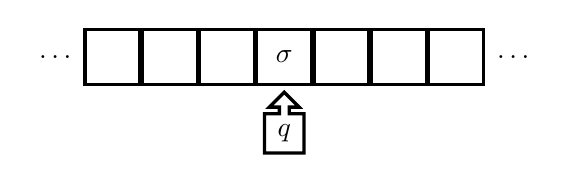
\begin{tikzpicture}
\tikzstyle{every path}=[very thick]
\edef\sizetape{0.7cm}
\tikzstyle{tmtape}=[draw,minimum size=\sizetape]
\tikzstyle{tmhead}=[arrow box,draw,minimum size=.5cm,arrow box
arrows={north: .25cm}]
\begin{scope}[start chain=1 going right,node distance=-0.15mm]
 \node [on chain=1,tmtape,draw=none] {$\ldots$};
 \node [on chain=1,tmtape] {};
 \node [on chain=1,tmtape] {};
 \node [on chain=1,tmtape] {};
 \node [on chain=1,tmtape] (input) {$\sigma$};
 \node [on chain=1,tmtape] {};
 \node [on chain=1,tmtape] {};
 \node [on chain=1,tmtape] {};
 \node [on chain=1,tmtape,draw=none] {$\ldots$};
 \node [tmhead,yshift=-.6cm] at (input.south) (head) {$q$};
\end{scope}
\end{tikzpicture}
\end{center}

The transition function $\delta$ describes what the machine should do in this moment. If 
\[\delta(\sigma,q)=(\lambda,r,d)\]
Then the interpretation is that the machine erases $\sigma$, prints $\lambda$ in it's place, changes to state $r$, and moves the cursor either one cell to the right, one cell to the left, or stays still, depending on whether $d$ is 1,0, or -1 respectively. If $d=1$, then the intuitive picture in the next 'moment' would look like this:
\vspace{1cm}
\begin{center}
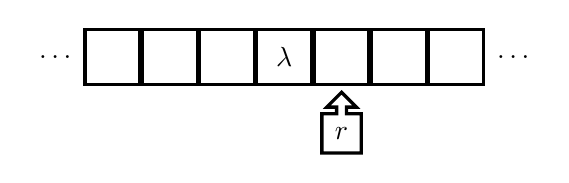
\begin{tikzpicture}
\tikzstyle{every path}=[very thick]
\edef\sizetape{0.7cm}
\tikzstyle{tmtape}=[draw,minimum size=\sizetape]
\tikzstyle{tmhead}=[arrow box,draw,minimum size=.5cm,arrow box
arrows={north: .25cm}]
\begin{scope}[start chain=1 going right,node distance=-0.15mm]
 \node [on chain=1,tmtape,draw=none] {$\ldots$};
 \node [on chain=1,tmtape] {};
 \node [on chain=1,tmtape] {};
 \node [on chain=1,tmtape] {};
 \node [on chain=1,tmtape] (input) {$\lambda$};
 \node [on chain=1,tmtape] (input) {};
 \node [on chain=1,tmtape] {};
 \node [on chain=1,tmtape] {};
 \node [on chain=1,tmtape,draw=none] {$\ldots$};
 \node [tmhead,yshift=-.6cm] at (input.south) (head) {$r$};
\end{scope}
\end{tikzpicture}
\end{center}
We now formalize the semantics of a Turing Machine. The key to this is the notion of a configuration.
\begin{definition}
A \textbf{configuration} of a Turing Machine M is a triplet $c=(T,q,z)$ where $T\in\Sigma^*$, $q\in Q$, and $z\in\mathbb{Z}$.  
\end{definition}
Intuitively, a configuration is a complete description of the state of a Turing Machine at any moment in `time'. The element T is called a \textbf{tape configuration}, and it documents what is printed on the tape, and where. It's important to note that the tape configuration is finite. To understand this, know that a bit further down we will have an initial tape configuration which is always finite, and the machine will always be at some finite number of steps from it's initial state. Thus there will always be a finite string such that everything to the right and to the left is nothing but 'blanks'. This region may shrink or expand, but it is always finite, and we can regard it as the portion of the tape which is 'in use'. This finite used region of tape is the tape configuration $T$. The state is self explanatory, and the natural number $z$ represents the current position of the cursor. There is an implicit assumption in declaring $z$ a natural number, as opposed to an integer. Since $z$ is nonnegative, this means that the tape only extends infinitely in \textit{one direction}. We will show later that this is nothing more than convention - allowing the tape of a Turing machine to be two-way adds nothing profound in the way of what is computationally possible or efficient. For any $n\in\mathbb{N}$, we let $T[n]$ denote the contents of the tape at position n.
\begin{definition}
Let $M=(\Sigma,Q,\delta)$ be a Turing Machine, and $c_1=(T_1,q_1,z_1)$, $c_2=(T_2,q_2,z_2)$ be configurations of M. We say that \textbf{$c_1$ yields $c_2$ in one step} and write $c_1 \overset{M}{\to} c_2$, if $\delta(T_1[z_1],q_1)=(T_2[z+d],q_2,d)$ and $z_2=z_1+d$. Inductively we can extend this definition in the obvious way to define what it means for $c_1$ to yield $c_2$ in k steps for any $k\in\mathbb{N}$, and we use $c_1 \overset{M^k}{\to} c_2$ to denote this.
\end{definition}
Thus we have a formal framework for describing 'steps' of a computation. Towards beginning the machine on some input, let $x\in(\Sigma-\{\sqcup\})^*$. We will call strings like this (that is, finite strings without any blanks), \textbf{inputs}, and we'll allow denote the \textbf{empty string} $\epsilon$ to also be an input. (Often we will refer to inputs as members of $\Sigma^*$, but this is an abuse of notation.) By $|x|$, we mean the \textbf{length} of x (that is, the number of characters in x). By $T_x$, we mean the tape configuration consisting of a single $\triangleright$, followed by $x$. Formally, $T_x[0]=\triangleright$, and $T_x[n]=x_{n-1}$ for $1\leq n \leq |x|+1$. 
\begin{definition}
We say that a Turing Machine M \textbf{halts in k steps} on an input $x\in\Sigma^*$, if for some tape configuration T, some cursor position z, and one of the two halting states $q_h \in \{q_y,q_n\}$, we have that $(T_x,q_0,0) \overset{M^k}{\to} (T,q_h,z)$. If the halting state is $q_y$, then we say that M \textbf{accepts} the input x, and if the halting state is $q_n$, then we say that M \textbf{rejects} the input x. We call the final tape congiguration the \textbf{output} of M, and write $M(x)=T$. If the machine never halts for any number of steps, then we write $M(x)=\nearrow$. 
\end{definition}
Before proceeding further we should come out and be upfront about some incoming hypocrisy regarding the so-called start symbol $\triangleright$. For a two sided infinite Turing machine, which is what we've defined as our standard, the $\triangleright$ only exists for our convenience. The more primal and fundamental form of the model we've described should be understood to make do without it, by having initial configurations begin with the first character of the input string rather than with a $\triangleright$. I have it in my definition because I found it helpful when I was being introduced to theory, and indeed it is sometimes very useful to have a symbol like this.

On the other hand, the blank symbol $\sqcup$ is absolutely fundamentally necessary, and in fact, it should be noted that this symbol has a very special role in the operation of any Turing machine, as it is the \textit{only} symbol which is ever allowed to occur infinitely often on the tape.

Now that we have a formal notion of what it machine to accept or reject an input, we can define what it means for a machine to truly solve a problem for us.
\begin{definition}
Let L be a language, and M be a Turing Machine. We say that M \textbf{decides} L if for all inputs $x\in\Sigma^\#$,
\[x\in L \Rightarrow \textrm{M accepts x in k steps for some k} \]
\[x \notin L \Rightarrow \textrm{M rejects x in k steps for some k}\]
\end{definition}
Note that we can't get away with simply writing the first condition with an $\iff$ and have an equivalent definition, since the machine may \textit{neither} accept \textit{nor} reject an input. The machine may simply trail on forever, never reaching a conclusion.
\begin{definition}
    If a language/decision problem $L$ is decidable by a Turing machine, we say that the language is \textbf{recursive}. Alternatively, we say that it is \textbf{decidable}, or \textbf{computable}. We call the set of all recursive languages \textbf{R}.
\end{definition}
Before moving on, we extend our definition of Turing machines to machines which are allowed multiple tape 'strings'. This extension is equivalent to the original model in it's capabilities, and takes the idea of a Turing machine from something abstract and foreign to one which will, with a bit of practice, quickly feel startlingly natural.
\begin{definition}
A \textbf{k-string Turing machine} is a triple $M=(\Sigma,Q,\delta)$, with $\Sigma$ and Q just as before. The only thing that is different is the transition function. Now, $\delta: \Sigma^k \times Q \to \Sigma^k \times Q \times \{-1,0,1\}^k$.
\end{definition}
The interpretation is that we now have multiple strings of tape, and multiple cursors positions to keep track of. At any single step, we are reading k symbols, and we are allowed to alter all of them in a single step before moving the k cursors left or right independently of each other. Configurations are just as before, except not we need k integers to keep track of cursor positions, and k strings of tape. Thus, the configurations of a k-string Turing machine are (2k+1)-tuples
\[c=(T_1,T_2,T_3,...,T_k,q,z_1,z_2,z_3,...,z_k) \]

We would still like for our inputs and outputs to be single strings, rather than vectors, so we take as the output only the contents of the last string of the machine, and record inputs on the first. Thus, for an input string $x\in \Sigma^\#$, our initial configuration would look like
\[c_x=(T_x,\epsilon, \epsilon,...,\epsilon,q_0,0,0,0,...,0) \]
Where $\epsilon$ denotes the tape configuration consisting of a $\triangleright$ followed by nothing but blanks. It should be obvious that adding multiple strings would provide a noticable boost in efficiency over single string machines. We will show shortly that this boost is not particularly significant. Before that we need to discuss in a bit more detail the philosophy of what we're actually trying to do here. 

\subsection{Operationalizing Difficulty: Time and Space}
What we are interested in is, in general, analyzing the \textit{difficulty} of computational problem. What \textit{is} difficulty? 

We should first note that in some sense, we talk about difficulty as a quantity. We talk about \textit{how difficult} something is. We say that this problem is \textit{more difficult} than some other problem. This is our initial assumption - difficulty is a quantity.

As a quantity, difficulty is still more complicated than most others. While we haven't proven that they exist yet, it can certainly be said that any problem which isn't computable is more difficult in a sense than any problem which \textit{is} computable. So in some sense, the problems which aren't computable are going to be \textit{infinitely} difficult. And yet, we will see that we are still able to measure and categorize tiers of difficulty nonetheless. It stands to assume then that difficulty as a quantity is more deeply connected to the generalization of the natural numbers known as the ordinal numbers - numbers which proceed past infinity. This ordinal property of difficulty can in some sense be traced to it's fundamental subjectivity. What is difficult in one sense might be easy in another sense. If a problem is impossible for normal computers, it may nonetheless be possible for a computer which has been equipped a certain special additional property. 

We will get to this, but primarily we will be interested in the difficulty of problems which \textit{are} computable, and in this sense we can think of difficulty as a distinct finite number. Even here, difficulty is a \textit{fuzzy concept}. It's presence was known before we even realized that it was a quantity, making it fundamentally different to the quantities that mathematicians and physicists are typically used to dealing with; who's definitions are baked into their method of measurement. For inspiration then, we turn to the social scientists, who are more used to dealing with this sort of thing. 

A psychologist wishes to analyze quantities like difficulty all of the time. They have words like isolation, alienation, greed, dominance - character traits which are clearly quantities and clearly philosophically valid ideas, but which nonetheless exist with no clear 'ruler' for measuring them. Nonetheless, the psychologist or sociologist wants to do controlled experiments just like any other scientist. They want to test hypotheses such as ``The social isolation of individuals increases proportionally to the length of the working day.''

I believe that the social scientists accomplish this by forming an \textit{operational} definition of alienation. What they do is define some material, measurable behaviors which can reasonably be \textit{associated} with social isolation. For example, suppose they decide to track the lives of 30 individuals, 15 of which work 12 hour days, and 15 of which work 8 hour days. For each person in the experiment, the scientist decides to measure, say, the amount of time spent conversing with friends and family outside of work. While this is not a concrete measure of isolation by any means, it can reasonably be argued that the results say something meaningful about isolation in general, and more importantly, \textit{very few would argue that} time spent talking with friends would decrease with isolation. As other social scientists create their own operational definitions for social isolation and conduct similar experiments, the aggregate can prove results through an exhaustive inability to falsify, arguable just as well as a physicist can prove results about their more 'concrete' quantities such as charge and mass. We will define several types of resources for which large amounts could reasonably be seen as signs of high difficulty. 

How can we form an operational definition for the difficulty of a computational problem? The gateway lies in the computational model. Suppose we have a Turing machine which decides a problem for us. Implicit to this model are certain resources which can be monitored. Number of steps, for instance, or amount of 'scratch paper' used. There are many more. Just as 'amount of time spent talking to friends and family' can be used in the negative for 'measuring' social alienation, the \textbf{runtime} of a Turing machine - number of steps which the machine takes to complete it's computation, can be used in the positive to 'measure' the difficulty of a problem. There is here still a complication though. 

Tracking the resource use of a specific computation isn't good enough to measure the difficulty of an entire problem. Problems, as we've defined them, involve infinitely many computations - one for any problem for which the answer is yes or no. 

Since any problem contains an infinite number of possible instances, in order to analyze the feasibility of a problem, we need to look at how resource requirements go up relative to how complicated the instance of the problem is. There is probably no objection to assuming that, as a rule of thumb, the larger the \textit{length} of an input is, the more demanding an instance of the problem becomes. If an input is long, we should expect that deciding if $x\in L$ will be more resource intensive than if the input was short, \textit{regardless} of what resource is being considered.

Thus, to measure the feasibility or difficulty of a problem, we need to define a resource of interest within a particular model of computation (for our purposes, the Turing model), and then track how quickly the use of that resource gets out of hand, as the input length increases. One of the primary advantages of the Turing model is that two resources which feel very natural to think about as scaling with difficulty feel just as natural to track within the model - time and space. We'll begin with time.

\begin{definition}
Let M be a Turing machine which, for some input x, halts after t steps. Then we say that the \textbf{time required by M on input x is t}. We say that \textbf{M operates in time $f(n)$}. if, for any string x, the time required by M on x is at most $f(|x|)$. 
\end{definition}

Note that our definition here implicitly is concerned with `worst-case' performance, in that the function $f$ is characterizes the machine $M$ as an upper bound. If we had replaced the words `at most' with 'at least' we would instead be concerned with `best-case' performance. Best-case, worst-case, and even average-case performance are all worthy of consideration. However, worst-case is the place to begin, and in many senses the most important of the three.

Suppose that $L_1$ and $L_2$ are problems which are computed by Turing machines operating in time $f(n)$, $g(n)$ respectively, and that these are the best known Turing machines which solve the problem. To compare the difficulty of these problems is to compare the \textit{growth rates of these two functions $f$ and $g$}. But now there is some question of how to compare these two functions. For instance, suppose that $g(n) = f(n)+1$. Then it is true that $g(n)$ is always bigger, but is $L_2$ really a more difficult problem than $L_2$? Certainly not. One extra step per computation is meaningless in the grand scheme of things. We would wish in this case to view the problems as $L_2$ and $L_1$ to be in the same general difficulty class. 

The same decision will be made in the case of $g(n) = cf(n)$ for some positive constant $c$. The decision to view problems like this as 'the same' difficulty is more questionable, but in the end just as well justified by the fact that by utilizing a larger alphabet, we can improve the performance of any Turing machine for \textit{arbitrary} amounts of linear speedup. We won't prove it in these notes, but we will state it for the record, and prove what is in some sense the inverse result shortly. (A full proof can be found in \cite{papadimitriouComputationalComplexity1994}.)

\begin{theorem}[The Linear Speedup Theorem]
	Suppose that $L$ is decidable by a Turing machine $M$ which operates in time $f(n)$. Then for any $\epsilon > 0$, there exists a Turing machine $M'$ with a larger alphabet than $M$ which operates in time $\epsilon f(n)+n+2$.
\end{theorem}
Practically any nontrivial problem is going to take more than $n$ steps to solve, since it always takes \textit{at least} $n$ steps to just scan the input. Any machine which operates in time less than $n$ would have to be populated by questions which can be answered without even looking at the input, hence the triviality.

Recall from calculus that two functions $f(n)$ and $g(n)$ are \textbf{comparable} if  the $f(n) = cg(n)$ for some constant $c$ - that is to say, $\lim_{n \to \infty} \frac{f(n)}{g(n)} = c$. It follows from the linear speedup theorem that we should view problems which are solvable by Turing machines operating in comparable amounts of time should be seen as 'the same' difficulty.

\subsubsection{Big-Oh}

Thus, in complexity theory, we are concerned exclusively with \textit{general classes} of growth rates, rather than specifics. To help us talk about things more simply, we define what is known as big $O$ notation, as well as some other things for later.
\begin{definition}[Big O]
Let $f,g:\mathbb{N} \to \mathbb{R}$. We say that \textbf{$f(n) \in O(g(n))$} if there exists a $c \in \mathbb{R}$ such that for all $n \in \mathbb{N}$, we have $f(n) \leq cg(n)$. 
\end{definition}
It's impossible to tell a difference, but that O is supposed to actually be the Greek letter capital omicron.
\begin{definition}[Little o]
	Let $f,g:\mathbb{N} \to \mathbb{R}$. We say that $f(n) \in o(g(n))$ if 
	\[\lim_{n \to \infty}\frac{f(n)}{g(n)} = 0 \]
\end{definition}

Usually we only care about $O$ and $o$ for functions which are positive and nondecreasing, and we will assume this is always the case unless otherwise noted. To point out some differences between these two things, first note that any $g(n)$ is \textit{always} in $O(g(n))$, but \textit{never} in $o(g(n))$. Also note that $o(g(n)) \subseteq O(g(n))$ Think of the difference between $O$ and $o$ as being akin to the difference between $\leq$ and $<$, but for growth rates. If $a < b$, then $a \leq b$, but obviously not the other way around. For big-O, functions in $O(g(n))$ grow \textit{incomparably slow or comparably fast} to $g(n)$. For little-o, functions in $o(g(n))$ grow \textit{incomparably slow}, nothing in $o(g(n))$ is allowed to match $g(n)$ in terms of growth rates.

\begin{definition}[Big $\Omega$]
	Let $f,g: \mathbb{N} \to \mathbb{R}$. We say that $f(n) \in \Omega(g(n))$ if there exists a positive $c \in \mathbb{R}$ such that $f(n) \geq cg(n)$.  
\end{definition} 

$\Omega(f)$ is $O(f)$'s sunny, optimistic, and often neglected sister. The idea is that $g(n) \in \Omega(f(n))$ grow \textit{comparably fast or incomparably faster} than $f$. So we take functions in $O(f)$ to be 'slower or similar' to $f$, and functions in $\Omega(f)$ to be 'faster or similar' to $f$. In this way, $\Omega$ will be useful to discuss \textit{best-case} performance, just as $O$ will be used to discuss worst-case. Discussion of best-case performance in complexity theory would amount to discussion of the \textit{optimality} of an algorithm - a proof that there is nothing better. Proofs of these kinds of claims are hard and rare, and so $\Omega$ tends to significantly less use than her brother. (For the record, the $O$ and $o$ in the notation are technically Greek capital and lowercase omicrom, but this looks identical to a regular o or O in the English alphabet.)

A \textbf{complexity class} is any nonempty proper subset of \textbf{R}. This is \textit{not} going to be a completely rigorous definition. For now though, this will do. We will make this more precise later.
\begin{definition}
	 For any function $f:\mathbb{N} \to \mathbb{R}$, let \textbf{TIME($f(n)$)} denote the class of languages L such that there exists a Turing machine M which decides L, operates in time $g(n)$, for some $g \in O(f)$
\end{definition}
So \textbf{TIME}$(f(n))$ is the set of all decision problems which are decidable by an algorithm which operates in time \textit{less than or equal to} $cf(n)$ for some $c$. Note that $f(n)$ could be $2^n$, and our problem might be solvable by an algorithm which works in linear time, and this language would still be in \textbf{TIME}$(2^n)$. Again this hearkens to the fact that in complexity theory, we are interested primarily (but not exclusively) in \textit{worst-case complexity}. If it's better, that's great, but the concern of the theory revolves around being 'no worse than'. We summarize this formally with a simple fact:
\begin{fact}
	If $f(n) \in O(g(n))$, then \textbf{TIME}$(f(n)) \subseteq \textbf{TIME}(g(n))$ 
\end{fact}
Next we turn to an inspection of the second natural resource associated with the Turing model - space. to start, picture yourself sitting at a desk, performing some long computation. You have a sheet of paper with the input, and a specific sheet to record the output onto, and you are blindly following some set of instructions to produce an output. Two obvious 'resources' should come to mind. One of these resources is the amount of time the computation takes, which we have formally captured above. The other is the amount of \textit{scratch paper} you need. 

Space is an interesting resource, because it has a fascinating inverse relationship with time. To illustrate this, let's consider the basic grade school algorithm we are taught to compute the sum of two numbers. Suppose we want to add the numbers 346 and 89. Our 'scratchwork' would look something like this:
\begin{center}
\begin{tabular}{c@{\,}c@{\,}c@{\,}c}
  & 1 & 1 &   \\
  & 3 & 4 & 6 \\
+ &   & 8 & 9 \\ 
\hline
  & 5 & 3 & 5 \\
\end{tabular}
\end{center}

In considering space complexity, the + sign and the line separating summands from sum are completely unnecessary and shouldn't be considered. Nor should the two numbers we are adding or the final output. (Remember, we are only considering the amount of scratch paper we need, and the input/output is on a separate page). Without these, it would seem like the only extra space needed are for the two carry bits. If we're given two numbers, the bigger of which has length, say, n, then the input can be taken to be of length 2n, and the maximum number of carry bits that we might possibly need is n-1. It would seem like our basic grade school addition algorithm operates in linear space, O(n).

But we don't really \textit{need} n-1 bits of space, do we? Once we use the carry bit and move leftward to the next digit, we won't need the old carry bit anymore. \textit{Provided we don't value our time, we could simply reuse that space}. We could leave the bit as a 1 if we need to carry another bit in the next step, or \textit{erase it} and replace it with a 0 if we don't. Again, \textit{provided we don't care about time constraints}, addition is actually uses only a \textit{single bit} of space!

We will see many more examples of this dynamic at play. To summarize, space as a resource is fundamentally different than time in that it is \textit{reusable}, and therefore, \textit{at the cost of time}, we can \textit{usually} save space. How much space can we save in general? It seems like the answer to this questions should vary wildly depending on the algorithm, so perhaps we should reword the question: What is the \textit{maximum} amount of space that we could \textit{possibly} save? The answer to this question seems to be exponential.  

In order to properly exclude the input and output in considerations of space, we make use of multiple strings. We will append extra strings to be reserved as input and output. We want to make damn sure that nothing worth considering ever happens on these two strings, so we take measures in the next definition to make sure that the input string is \textit{read only}, and the output string is \textit{write only}.
\begin{definition}
A \textbf{k-string Turing machine with input/output} is a k+2-string Turing machine with the condition that if $\delta(\sigma_1,\sigma_2,...,\sigma_{k+2},q)=(\rho_1,\rho_2,...,\rho_{k+2},r,...,d_1,d_2,...,d_k)$, then $\sigma_1 = \rho_1$ and $i_k \neq -1$
\end{definition}

This condition ensures that no symbols of the input string can be overwritten, and that the cursor of the output string can only move forward. 
The definitions for time complexity easily apply to k-string machines with no alterations. We are ready to define the space used in a computation for these types of machines. After doing so we can state a theorem which confirms that there is no loss of generality in viewing any ordinary Turing machine as a Turing machine with input/output, assuring that this definition can be applied generally.
\begin{definition}
Let M be a single string Turing machine with input/output, and suppose that M halts on input $x \in \Sigma^\#-\{\sqcup\}$ after t steps. For $l=0,...,t$, let $c_l = (T_1,...,T_{k+2},q,z_1,...,z_{k+2})$ denote the configuration of M, initially in configuration $c_x$, after l steps. Then the \textbf{space required by M on input x} is the number
\[\max_{l\leq t}\{\sum_{i=2}^{k+1}|T_i|\} \] 
Note that for a Turing machine with only one work string, this amounts to simply the maximum length of that string at any step, i.e. $\max_{l \leq t}(|T_2|)$. For a function $f:\mathbb{N}\to \mathbb{R}$, we say that \textbf{M operates in space $f(n)$} if for any input $x \in \Sigma^*-\{\sqcup\}$, the space required by M on x is at most $f(|x|)$. 
We also define the class $\bm{SPACE}(f(n))$ to be the collection languages L which are decidable by some Turing machine M operating in space $g(n)$, for some $g \in O(f(n))$. Just as we noted above, it is obvious that for any $g(n) \in O(f(n))$, $\bm{SPACE}(g(n)) \subseteq \bm{SPACE}(f(n))$.
\end{definition}
Now is as good a time as any to make an extremely simple but nonetheless important observation, one which would appear deep for computer scientists used to more complicated models of computation, but for Turing machines is clear as day:
\begin{fact}
For any function $f:\mathbb{N} \to \mathbb{R}$, 
\[\textrm{\textbf{TIME}}(f(n)) \subseteq \textrm{\textbf{SPACE}}(f(n)) \]
\end{fact}
\begin{proof}
If L is decided by a k-string Turing machine in $f(n)$ steps, then there is certainly no way to move more than $kf(n) \in O(f(n))$ tape cells in either direction!
\end{proof}
This is as far as we're going to go for now with respect to complexity theory. Before we can talk in detail about this topic, we need to note some basic things about Turing machines. We went to the trouble early on of defining these things because it will be important to analyze resource use as we go through the first wave of basic results, which we turn to now.

Consider the Turing machine $M = (\{\triangleright,\sqcup,0,1\},\{s,h,q,q_0,q_1\},\delta)$, with $s$ the starting state and $h$ a halting state, and $\delta$ defined as follows:
\begin{center}
\begin{tabular}{ |c c|c| } 
 \hline
 State & Symbol & Output of $\delta$ \\ 
 \hline
 $s$ & $0$ & $(s,0,1)$ \\ 
 $s$ & $1$ & $(s,1,1)$ \\ 
 $s$ & $\sqcup$ & $(q,\sqcup,-1)$ \\
 $s$ & $\triangleright$ & $(s,\triangleright,1)$ \\
 $q$ & $0$ & $(q_0,\sqcup,1)$ \\
 $q$ & $1$ & $(q_1,\sqcup,1)$ \\
 $q$ & $\sqcup$ & $(q,\sqcup,0)$ \\
 $q$ & $\triangleright$ & $(h,\triangleright,1)$ \\
 $q_0$ & $0$ & $(s,0,-1)$ \\
 $q_0$ & $1$ & $(s,0,-1)$ \\
 $q_0$ & $\sqcup$ & $(s,0,-1)$ \\
 $q_0$ & $\triangleright$ & $(h,\triangleright,1)$ \\
 $q_1$ & $0$ & $(s,1,-1)$ \\
 $q_1$ & $1$ & $(s,1,-1)$ \\
 $q_1$ & $\sqcup$ & $(s,1,-1)$ \\
 $q_1$ & $\triangleright$ & $(h,\triangleright,1)$ \\
 \hline
\end{tabular}
\end{center}
The reader should show to themselves with a simple example that this machine simple creates a single blank space in between the starting $\triangleright$ and the input $x$, and then halts. That is to say, $M(x) = \sqcup x$. This is a useless program on it's own, but it serves a smaller 'building' block in the sense that it would be nice if we could use this within the context of building something bigger. Perhaps we are designing a Turing machine which at some point needs to create a space somewhere on it's work string. We would detect the need for this of course via finding a particular symbol-state pair, call them $\sigma$ and $v$ respectively. What we could do is define $5$ new states for the machine we are building, corresponding to the $5$ in this machine above and one more, call it $v$, as well as the new 'special' symbol, $\underline{\sigma}$, where $\sigma$ is the symbol for which you want everything to the right of it moved over. For simplicity, we will assume that none of the letters used in the $Q$ above have been used yet. First, we have the command $\delta(\sigma,v) = (\underline{\sigma},s,0)$. From here, everything is defined \textit{exactly} as above. The 'starting state' $s$ now takes the form of an initialization of a subroutine, and the 'halting state' $h$ would take the form of a completion of that subroutine. 

We will need this subroutine shortly for a specific proof, but more generally it points to a principle which we will can make extensive use of going forward:
\begin{center}
	In principle, given we have defined previously a machine which produces a specific function, we can without any extra justification use this machine as a subroutine in the creation of larger programs. 
\end{center}
	By this same principle we also but we also have the following important lemma:
\begin{lemma}
    Let $M_1,M_2$ be Turing machines. Then there exists a Turing machine $M$ such that for all $x$, $M(x) = M_2(M_1(x))$, where $M(x)$ is defined as $\nearrow$ whenever $M_1(x) = \nearrow$ as well as whenever $M_2(M_1(x)) = \nearrow$. 
\end{lemma}
\begin{proof}
    Let $Q_1$ and $Q_2$ represent the states of $M_1$ and $M_2$, and let $\delta_1$ and $\delta_2$ the transition functions, and WLOG suppose that $Q_1$ and $Q_2$ are disjoint. 
    Also WLOG assume that the $M_1$ leaves the initial $\triangleright$ symbol alone, so the output can always be expected to lead with it. For the machine $M$, we let the $Q=Q_1 \cup Q_2$, and define $\delta = \delta_1$ for any state/symbol pair with a state belonging to $Q_1$, \textit{with the exception of $Q_1$'s halting state}, call it $q_h^1$. 
    On this state, define $\delta({q_h}^1,b) = ({q_h}^1,b,-1)$ for any symbol $b \neq \triangleright$, and $\delta(q_h^1,\triangleright)=(q_{s_2},\triangleright,0)$, where $q_{s_2}$ is the starting state for $M_2$. We then define $\delta = \delta_2$ for all state-symbol pairs with states in $Q_2$, and have the halting state for $M_2$, $q_h^2$, act as the halting state for $M$. It should be clear that $M$ performs as desired. 
\end{proof}
\begin{exercise}
	Modify the Turing machine we described earlier that creates spaces in the following way: Define a two-string Turing machine which, when initialized with a binary coding of an integer $n$ in the top tape-string, and a string $x$ in the bottom string, creates $n$ spaces between the $\triangleright$ and the $x$, and then halts. That is to say, we are modifying the space-creating program to move the string $x$ to the right by a specified distance. Describe a second Turing machine which moves the string $x$ a desired number of spaces to the left (without regard to the $\triangleright$). These machines as subroutines will be useful in constructing a universal Turing machine, which will be our next objective. 
\end{exercise}

\subsection{Robustness Theorems}
We now take some time to develop our model, proving various facts which when taken together demonstrate a certain peculiar robustness which the model possesses. To this end we begin by defining what it means for two machines to be functionally the same.
\begin{definition}
	We say that two Turing machines $M_1,M_2$ are \textbf{equivalent} if for all strings $x$, $M_1(x) = M_2(x)$, and that $M_1$ accepts/rejects an input $x$ iff $M_2$ accepts/rejects $x$. 
\end{definition} 
\begin{lemma}[Staying still is unnecessary]
	For any Turing machine $M$, there exists an equivalent Turing machine $M'$ with transition function $\delta'$ such that the third coordinate of $\delta(\sigma,q)$ is strictly nonzero. That is to say, the cursor of the machine will never stay still.
\end{lemma}
\begin{proof}
	This is easy. Let $M = (\Sigma,Q = \{q_1,q_2,...,q_n\},\delta)$. The machine $M'$ will have the same alphabet, and $n$ extra states $s_1,...,s_n$ which weren't already in $Q$. Suppose that $\delta(\sigma,q_i) = (\sigma',q_j,0)$. For this, let $\delta'(\sigma,q_i) = (\sigma',s_j,1)$, and $\delta(\sigma,s_j) = (\sigma,q_j,-1)$. If $\delta(\sigma,q) = (\sigma',q',d)$ with $d \neq 0$, then we simply let $\delta'(\sigma,q) = \delta(\sigma,q)$. Clearly $M'$ performs identically to $M$, except that wherever $M$'s cursor would stay still, $M$ will take an extra step to have it's cursor move one cell forward followed by one step backward, and then continue onward as normal. Obviously this uses no extra space at all. In considering time, the worst case would be the situation in which the cursor perpetually stays still in the original machine's computation. In this instance, we would be adding two extra steps per step of the original machine, making the computation take $3$ times as long. Thus if the original machine operates in time $O(n)$, the new machine will operate in time $O(3n) = O(n)$ as well. 
\end{proof}
\begin{corollary}
	$\bm{R}$ is the same class regardless of whether or not our Turing machine model has the ability to 'stay still', as is the class $\bm{TIME}(f(n))$ and $\bm{SPACE}(f(n))$ for any function $f$. 
\end{corollary}
When we defined the class \textbf{R}, as well as $\bm{TIME}(f(n))$ and $\bm{SPACE}(f(n))$, we were a bit aloof about representation. Suppose that $\Sigma = \{0,1,2,3,4,5,6,7,8,9\}$ and we have a language over this which is computable. Then it stands to reason that the same language with numbers represented in binary rather than decimal, that is to say over the alphabet $\{0,1\}$, would also be computable. Are there to be two of 'the same language' in \textbf{R} then? To avoid this kind of confusion, we would like to fix a specific alphabet and a particular encoding of problems in other alphabets so that they have concrete representations over this one.

For any alphabet $\Sigma$, define the \textbf{standard unary coding} of $\Sigma$ to be the unary coding of symbols in $\Sigma$ with a single arbitrary symbol (label it $1$, though in the following proof it will be a $\triangleright$) padded with enough of some other arbitrary symbol (label it $0$, though for our purposes it will be a $\sqcup$ to make all code words the same length. For example, if $\Sigma = \{a,b,c\}$, then the standard unary coding would be $\{001,011,111\}$. For reasons that will become clear shortly, whenever the language being coded includes a machine blank $\sqcup$, we will assume that this is encoded as the string of all zeros $00\ldots 0$. Under the standard unary encoding, any language over $\Sigma$ has a one to one correspondence with one over the alphabet $\{0,1\}$, and each string length will be exactly $|\Sigma|$ times longer than those strings in $\Sigma$. 
\begin{theorem}[More than two symbols is unnecessary]
	For any Turing machine $M$ over the alphabet $\Sigma$, there exists a Turing machine $M'$ over the alphabet $\{0,1\}$ which is equivalent to $M$ \textit{up to} the standard unary encoding of inputs and outputs. $0$ will be regarded as $M$'s blank symbol, in the sense that it will be the unique symbol of $M$'s alphabet which is allowed to occur infinitely often on the tape. 
\end{theorem}
\begin{proof}
	By the last lemma, we may WLOG assume that the machine $M$ never has it's cursor stay still. Let $\delta$ be the transition function for $M$, and $Q = \{1,2,...,l\}$ be the set of states of $M$. The idea is to represent tape cells in $M$'s computation via multiple 'actual' tape cells. 
	The machine $M$ will begin with the input $x$ encoded in the way described above, with the cursor pointed at the first symbol of the first encoded symbol of $x$. A single cell of the origitnal machine will be represented by a block of $s$ cells, where $|\Sigma| = s$. The idea will be to simulate a step of the machine $M$ in the following way: The machine will always begin a simulated step with the cursor pointed at the leftmost symbol of an encoding. First, it moves to the end of the block, \textit{reading} through the block's contents in order to determine the symbol being looked at. Then, it will back up again, \textit{writing} in the code for the new symbol which is supposed to replace it. Finally, it \textit{moves} either to the previous cell or the next cell depending on what direction the cursor of the simulated machine is suppose to go. The reader is encouraged to try and write the details of this themselves before looking through my construction. 

	For the read phase, we will define the states $r_{0,0,1},r_{0,0,2},...,r_{s,s,l}$. The final subindex of $r$ holds the current state of the simulated machine. The first subindex counts how far through the block we've moved, while the second subindex counts the number of $1$'s specifically, so as to determine the code number for the symbol being stored there. To this end, for any state $q$, and any $i,j <s$,  we define $\delta'(0,r_{i,j,q}) = (0,r_{i+1,j,q},1)$, and $\delta'(1,r_{i,j,q}) = (1,r_{i+1,j+1,q},1)$. The effect of these definitions will be to eventually land the cursor of our machine one cell to the right of the final cell of the block, with the middle index holding the number representing the symbol being looked at. 

	For the write phase, we define the states $w_{0,0,1,-1},w_{0,0,1,1},w_{0,0,2,-1},...,w_{s,s,l,-1},w_{s,s,l,1}$. Suppose $\delta(\sigma,q) = (\lambda,p,d)$, with $a$ is the number of $1$'s encoding a $\sigma$, and $b$ the number of $1$'s encoding a $\lambda$. Then the transition from read to write for this particular $a$ and $q$ will be defined by $\delta'(0,r_{s,a,q}) = (0,w_{s,b,p,d},-1)$, and $\delta'(1,r_{s,a,q}) = (1,w_{s,b,p,d},-1)$. From here, we begin moving left, disregarding the contents of the block we are moving through, recording $1$'s while decrementing the second index $b$ until it reaches $0$ while also decrementing the first, and recording $0$'s until the end of the block is reached after the second index reaches $0$. To this end, for $\gamma \in \{0,1\}$, and for $i,j>0$, define $\delta'(\gamma,w_{i,j,p,d}) = (1,w_{i-1,j-1,p,d},-1)$, and for $i>0,j=0$ define $\delta'(\gamma,w_{i,j,p,d}) = (0,w_{i-1,0,p,d},-1)$. This will leave us in the state $w_{0,0,p,d}$, with our cursor pointing at the final symbol of the block left of the one we have been working on. At this point, the machine $M'$ can inspect $p$ and determine if it's a halting state. If it is, then this is where we halt, in the corresponding halting state for $M'$. 

	Otherwise, we need to move to an adjacent cell, and so we need to enter and describe a move phase. In the case $d=1$ we need to move forward $s+1$ cells to reach the beginning of the block right of the one we were just working on, and if $d=-1$ then we need to move backward $s-1$ cells to reach the beginning of the block we are currently inhabiting. For the job we define the forward movement states $f_{1,1},f_{1,2},...,f_{s,l}$, and the backward movement states $b_{1,1},...,b_{s-2,l}$. For the transition from write to move, have $\delta'(0,w_{0,0,p,1}) = (0,f_{1,p},1),\delta'(1,w_{0,0,p,1}) = (1,f_{1,p},1), \delta'(0,w_{0,0,p,-1}) = (0,b_{1,p},-1)$, and $\delta'(1,w_{0,0,p,-1}) = (1,b_{1,p},-1)$ for any $p = 1,...,l$. Then, for the forward case, with $i=1,...,s-1$, have $\delta'(0,f_{i,p}) = (0,f_{i+1,p},1),\delta'(1,f_{i,p}) = (1,f_{i+1,p},1)$, which will have the effect of moving the cursor to the final cell of the block we were operating on before, from which we transition to a new read phase by $\delta'(0,f_{s,p}) = (0,r_{0,0,p},1),\delta'(0,f_{s,p}) = (0,r_{0,0,p},1)$. For the backward case, for $i=1,...,s-3$, have $\delta'(0,b_{i,p}) = (0,b_{i+1,p},-1),\delta'(1,b_{i,p}) = (1,b_{i+1,p},-1)$, and then finally $\delta(0,b_{s-2,p}) = (0,r_{0,0,p},-1)$. This completes the description of simulating a step of $M$, as well as completely defines the transition function $\delta'$ on all pairs of interest, and thus the construction of $M'$.

	It remains to investigate the complexity of what we just described. Suppose that the machine $M$ operates in time $f(n)$ and spaces $g(n)$. Then it should be clear that our new machine operates in time approximately $3sf(n)$ and space $g(n)$, and thus both machines operate in time $O(f(n))$ and $O(g(n))$. At least as far as the rate of difficulty which scales with the size of the input, there is no meaningful loss of efficiency. 
\end{proof}
\begin{corollary}
	The classes $\bm{R},\bm{TIME}(f(n))$, and $\bm{SPACE}(f(n))$ are always the same collection set up to a standardized one-to-one correspondence. That is to say, if we define, say $\bm{TIME}(f(n))$ to be the class of languages computable by a Turing machine operating over the alphabet $\{a,b,c,d,e\}$, then there is a one-to-one correspondence between computable languages over this alphabet and computable languages over $\{0,1\}$, and the restriction of that mapping to any of the above classes remains a bijection between the smaller classes for any $f(n)$. 
\end{corollary} 
The end result of our discussion of alphabets is that we can without loss of generality for rest of these notes assume that all of the languages that we discuss are the same objects - simply collections of finite binary strings. Furthermore, we may prove results about this now concrete class of objects by using \textit{whatever alphabet we want} when building Turing machines, knowing that any construction can be converted into a construction for the fixed binary alphabet. Keep in mind that this means that our convention of including a $\triangleright$ in every Turing machine is completely harmless and inconsequential.

Our next result concerns the need for how our tape extends infinitely. Currently our definition entails a machine whose 'tape' extends infinitely both left and right. We can define a machine whose tape only extends infinitely in one direction as a restriction of our current model, in the following way:
\begin{definition}
	A \textbf{unidirectional} Turing machine is a Turing machine $M = (\Sigma,Q,\delta)$ such that if $\delta(\triangleright,q) = (\sigma,p,d)$, then $\sigma = \triangleright$, and $d \neq -1$. Thus, the $\triangleright$ symbol takes on special meaning in that it can't be passed over on the left, nor can it be overwritten. Under our given input convention, this means that the cursor can never retreat left of the starting position.
\end{definition}
As unidirectional Turing machines are a special case of regular Turing machines, it is trivially the case that any language decided by a unidirectional Turing machine can be decided by a Turing machine at no loss of resource efficiency. The following result shows the converse of this.
\begin{lemma}[Only need infinite tape in one direction]
	For any Turing machine $M$, there is an equivalent Turing machine $M'$ which is unidirectional and operates at the same big-O efficiency for space and time.
\end{lemma}
\begin{proof}
	The obvious way to accomplish the construction would be to design a Turing machine which implements our space-making subroutine every time it reaches a $\triangleright$ in a state which the original machine $M$ would want to move left from. However one can quickly see that a method like this would result in a machine which operates in time $O(nf(n))$, where $f(n)$ is the operating time of the original machine. In order to not lose any time a more sophisticated algorithm is necessary. 

	The idea is going to be to, in a similar manner to the standard bijection from the integers to the natural numbers, \textit{fold} the two sided tape in half, and interleave the positive and negative entries. Let $Q = \{q_1,q_2,...,q_l\}$ and assume that $q_l$ is the (without loss of generality only) halting state. be the set of states for the original machine. Instead of these states, we will include in $M'$ the states $q_1^+,q_1^-,q_2^+,q_2^-,...q_{l-1}^+,q_{l-1}^-$. We will also include what we will call the 'hop states' $i_{1,1}^+,i_{1,-1}^+,i_{2,1}^+,i_{2,-1}^-,...,i_{l-1,1}^+,i_{l-1,-1}^-$. The halting state $q_l$ will be the same for both machines. The idea is to have the machine $M'$ be in a $+$ mode or a $-$ mode, depending on whether the simulated machine $M$ is on right right or left 'half' of the tape. Past the starting $\triangleright$, we will interpret all odd cells as cells on the positive half of the tape, and all even cells as cells on the negative half. While in either the $+$ mode or the $-$ mode, the machine will mimic the behavior of $M$ except that it will 'hop' over a cell every time it moves, so as to stay on the correct tape cells (the intermediary hop phases are there to facilitate this jump). Whenever it detects a $\triangleright$, which we will assume is the only one, (we can do this by adding a second $\bar{triangleright}$ symbol to $M$ which is uses everywhere it would use an actual $\triangleright$ would be used normally, except for the input configuration, and appealing to the above fact about equivalence between alphabets) the machine $M'$ may or may not switch from one 'polarity' to the other, depending on the direction it's supposed to go. 

	We flesh this idea out now, beginning with the transition from a positive mode to a negative mode. Note that since positive cells are odd, we will only ever detect a $\triangleright$ during our intermediary hop states (the exact opposite will be true for the transition from negative to positive polarity). For the non-$\triangleright$ hops, define for $\sigma \neq \triangleright, d = 1,-1,j =1,...,l-1$, define $\delta'(\sigma,i_{j,d}^+) = (\sigma,q_j^+,d)$. For the polarity switch, define $\delta'(\triangleright,i_{j,-1}^+) = (\triangleright,i_{j,1}^-,1)$ (note that a $\triangleright$ can only be encountered during a positive hop state if $d=-1$). This transition puts the machine in a position where it thinks it is in the negative mode and needs to hop right, which will safely land it in the first negative cell and continue as usual. 

	The negative mode is a bit more complicated since we will only land on a $\triangleright$ when \textit{after} a hop. To deal with this we will lazily add in some more intermediary check states $c_1,c_2,...,c_{l-1}$. These will be defined by $\delta'(\sigma,c_j) = (\sigma,q_j^-,0)$ if $\sigma \neq \triangleright$, and $\delta'(\triangleright,c_j) = (\triangleright,q_j^+,1)$ otherwise. As for regular negative moves, if $\delta(\sigma,q) = (\lambda,q,1)$, then have $\delta'(\sigma,q_i^-) = (\lambda,i_{j,-1}^-,-1)$ and if $\delta'(\sigma,q_i) = (\lambda,q_j,-1)$ then have $\delta'(\sigma,q_i^-) = (\lambda,i_{j,1}^-,1)$. Note the directional flip - moving forward on the two sided tape while on the negative side amounts to moving \textit{closer} to the middle, and thus we need to move \textit{backward} on the simulating machine as if to approach closer to the $\triangleright$. Similarly moving backwards will amount to moving further forwards. As for the hops, define $\delta'(\sigma,i_{j,d}^-) = (\sigma,c_j,-d)$ (again noting the directional reversal). The effect of these instructions is to have a machine which mimics changes the symbol and state as it should, hops two cells in the direction it needs to, checks if it is seeing a $\triangleright$, and reacts accordingly.

	Finally, if $\delta(\sigma,q_i) = (\lambda,g_l,d)$ for some $\lambda,d$, then we don't need to worry about moving because we only need to replace the symbol and halt. For this reason define $\delta'(\sigma,g_i^+) = (\lambda,q_l,0)$, and $\delta'(\sigma,g_i^-) = (\lambda,q_l,0)$. This completes the construction of $\delta'$ for all relevant inputs, and thus \textit{almost} the construction of $M'$. 
(We need to talk about the initial configuration, but we will do this outside of the proof shortly.) Note that a single simulated step of $M$ is at most three steps for $M'$, and so at worst this machine $M'$ operates in time $3f(n) \in O(f(n))$ where $f(n)$ is the operating time of $M$, and with identical space efficiency.	
\end{proof}
There is a very slight complication of the above proof. Our convention is to have the machine start with the string $x$ written out as an input with the cursor on the starting $\triangleright$. That is to say, \textit{on the positive side of the tape}. If $x_1 x_2 \ldots x_n$ is the input string for the machine, then our above description only works on the condition that it begins with the initial tape configuration $\triangleright x_1 \sqcup x_2 \sqcup \ldots \sqcup x_n$. The same issue will apply to the output. Thus unless our Turing machine convention is to always be using a Turing machine with input/output, we will need to perform an initial subroutine which rewrites $x$ in the appropriate form, and then rewrites the output in the appropriate form following the computation's completion. This task can be accomplished in time $O(n^2)$ by making repeated use of our space creation subroutine, but that's a big time efficiency loss. The way I will deal with this is by simply copping out, and assuming that with all discussion of time/space efficiency classes, we will assume the model to be always fixed as single string Turing machines with input/output. (As we will see shortly, multiple string worktapes can be collapsed into a single one rather easily.)
\begin{corollary}
	For any $f(n)$, $\bm{TIME}(f(n))$, $\bm{SPACE}(f(n))$ are the same are the same regardless of whether the classes our Turing machines are one-sided or two-sided, as is $\bm{R}$. 
\end{corollary}
\begin{theorem}[More than $1$ string is unnecessary]
Given a k-string Turing machine M operating in time $f(n)$, there exists a single string Turing machine M' such that $M(x)=M'(x)$ for all $x\in \Sigma^*$ (and operating in time $O(f(n)^2)$, but we won't define time complexity until later.)
\end{theorem}
\begin{proof}
	By the previous lemma, we will assume that our $k-string$ Turing machine is 1-sided. In principle, a 1-sided Turing machine is just a two sided Turing machine with the special constraint that the transition function never moves left past any $\triangleright$ symbols (thus blocking the path). Thus we will make that assumption for the machine $M$. (TODO) Seeing the truth of the claim is simple in principle - we just need to cram all k-strings onto one string, which will involve adding new symbols as markers to divide them up. We will need subroutines to reconfigure the work string and to add space when more of a particular string needs to be used than has already been used, and we will make use of additional symbols - a copy of each of the symbols of the original machine - to keep track of where each cursor is. (By the lemma's we have so far, we can use as many more symbols as we want with the simulating machine.) We will proceed to formalize this idea. Let $M = (\Sigma,Q,\delta)$. The alphabet for our new machine will be $\Sigma' = \Sigma \cup \underline{\Sigma} \cup \{\triangleright',\triangleleft, \underline{\triangleright}',\underline{\triangleleft}\}$, where $\underline{\Sigma} = \{ \underline{\sigma}: \sigma \in \Sigma \}$.

	Note that single string Turing machines are initiated in exactly the same way as multi-string Turing machines - with the entire input in the top string, which in the case of a single string machine is the only string. Thus there is no need to discuss how to re-code inputs. What we will need to do is set up a single string workspace which is prepped to simulate the multiple strings. We will do this by first moving the entire input string one cell to the right, preceding it with a $\underline{\triangleright'}$, and then following up the input with the string $\triangleleft(\underline{\triangleright'},\triangleleft)^{k-1}\triangleleft$. The reader is invited to write out the details and show themselves that this can be done with $2k+2$ states additional to the original set $Q$.

	Once this setup phase is complete, the machine $M'$ can simulate a step of the original machine $M$ by scanning twice from left to right, and then back, gathering information in a similar manner to how we scanned many cells in order to simulate a single cell in our proof of the 2 character alphabet lemma. In the first scan, $M'$ gathers information on the $k$ symbols which would currently be 'looked at' by the original machine. Just like the many states we added in the alphabet lemma, we can have multiple 'subscript' states for each symbol of each string. It does this, and then backtracks to the beginning of the string by encountering the 'real' $\triangleright$. $M'$ can now make a second pass over the string, with the knowledge of what to replace the underlined characters with. Note that it is going to have to replace each underlined character with another underlined character (in the event that the cursor stays still) and otherwise with a non-underlined character. In the latter case, a second change will need to occur - the character to the left or the right of the underlined character will need to be replaced with it's underlined equivalent. Suppose that the newly underlined character is a $\triangleleft$. This would correspond to a yet-unused portion of one of the individual tape strings in the original computation, a 'new' $\sqcup$. In this case we must pause, and make room for this. Thus we must execute a 'subroutine' in which the entire string is moved right by one cell, up to and including the $\underline{\triangleleft}$, and a $\underline{\sqcup}$ is printed in it's former place. The Turing machine we explicitly defined above can do exactly this for us. Upon completing this second pass, we return back to the beginning of the string, and repeat the process. Thus a single step of the original $k$-string machine is simulated on the $k$ string machine.
	
    To analyze the complexity of the above, suppose that our original $k$-string machine $M$ halts in time $f(|x|)$. Note that in this time, none of the $k$-strings of $M$ will ever have more than $f(|x|)$ many non-blank cells. Thus the total length of the single string of the machine $M'$ is never longer than $k(f(|x|)+1)+1$. (The $1$ inside of the parenthesis is for each of the $\triangleleft$ symbols, while the final $1$ is for the single extra $\triangleleft$ at the end.) Thus up to constant multiples there is no space efficiency loss at all. Furthermore, in the worst case, simulating a single step of $M$ will involve two separate traversals from left to right and then back, taking $4k(f(|x|)+1)+4 = O(kf(|x|))$ steps, plus it will have to execute the space creating subroutine $k$ times. A bit of thought shows that this subroutine operates in linear time, and so this constitutes an additional $O(kf(|x|))$ many steps for each simulated step. Thus the total number of steps per simulated step is $O(kf(|x|))$, and since we have to execute $f(|x|)$ total steps, we have a simulation which works in time $O(k^2f(|x|)^2)$, or since $k$ is fixed, $O(f(|x|)^2)$. It can be shown by using a more complicated alphabet that in fact the $k^2$ term can be reduced to just a $k$ term. (See \cite{papadimitriouComputationalComplexity1994} exercise 2.8.6)
\end{proof}
\begin{corollary}
	As before, when we defined $\bm{TIME}(f(n))$, we ignored the number of strings that the machine had, and when we defined $\bm{SPACE}(f(n))$, we assumed a 3 string machine with a single work tape. Now apply more detail - define $\bm{TIME}_k(f(n))$ to be the class of problems decidable by a $k$-string Turing machine in time $O(f(n))$. Then for any $k$, $\bm{TIME}_k(f(n)) \subseteq \bm{TIME}_1(f(n)^2)$. It should also be obvious that $\bm{SPACE}_k(f(n)) = \bm{SPACE}_1(f(n))$ for any $k$, where $\bm{SPACE}_k(f(n))$ is defined to be the class of problems decidable in space $O(f(n))$ with $k+2$ strings, in which the first is a read-only input tape, the last is a write-only output tape, and the machine has $k$ work strings. And finally, of course, $\bm{R}$ is the same class for any number of tapes as well.
\end{corollary}
So while $k$-tape machines can't solve any problems that single tape machines can't, it still seems like they can potentially offer quadratic speedup. We can see an example of this speedup with the palindrome problem:
\begin{problem}
	The palindrome problem
	\begin{center}
		$PAL$: Given a string $x$, is it a palindrome? That is, is the sequence read backwards the same as if read forwards?
	\end{center}
\end{problem}
\begin{fact}
	$PAL \in \bm{TIME}_2(f(n))$, and $PAL \in \bm{TIME}_1((f(n))^2$
\end{fact}
\begin{proof}
	todo
\end{proof}
Amazingly, we also have the following:
\begin{theorem}
	\textit{Any} single string Turing machine which computes $PAL$ must operate in time $\Omega(n^2)$. 
\end{theorem}
\begin{proof}
	todo
\end{proof}
\begin{corollary}
	$PAL \notin \bm{TIME}_1(f(n))$. Thus, $\bm{TIME}_1(f(n)) \subset \bm{TIME}_2(f(n))$ - the containment is proper.
\end{corollary}
Thus through an exploration of this one simple problem, we've proven something very deep in general - parallel computing \textit{can} speedup (albeit to very limited degree) the computation of at least some problems, to a degree greater than anything that a single string machine can accomplish. It is unknown, at least to me, whether or not \textit{all} problems can be sped up in this way, however. (Research: Try speeding up a complete problem.) It is also unknown to me whether $\bm{TIME}_k(f(n))$ is proper in $\bm{TIME}_{k+1}(f(n))$ for \textit{any} k. 

Despite this result, it won't effect our discussion much. The classes we are centrally interested in are aggregates of many different time classes. Notably, $\bm{P}$ will be our general class which we will later see as the class of problems which are 'efficiently computable', and this class will include $\bm{TIME}(n^k)$ for any $k$, meaning smearing away the smaller differences. $\bm{P}$ itself will remain the same regardless of number of strings. 

Knowing that we can have as many 'rows' of tape as we want is what, at least to me, solidifies the Turing machine as the 'natural model'. Think of each row as a row on a sheet of graph paper. When imagining a program Turing machine, you need only imagine how you yourself would perform a computation on a sheet of graph paper, with a pencil. It is the one which is based not on some kind of metal contraption running on electricity, but instead is based on the idea of a person, sitting at a desk, doing arithmetic with a pencil. 

The results we've shown so far reveal the Turing model as one which is quite robust, but there is still one crucial aspect of them which may make them appear weaker than actual computers. The Turing machine's we've been describing are specially designed to solve specific problems. A modern computer, in contrast, when appropriately programmed, can solve any computable problem. We would like to produce a Turing machine with this same capability, one which we will call a \textbf{universal Turing machine}. 

Our universal Turing machine will be denoted $U$, and will be a machine which takes two inputs (separated by a blank). The first input will be a string which describes \textit{some other} Turing machine, $M$, and the second will be the desired input which we would like to have $M$ evaluate. That is, we would like $U(M,x) = M(x)$. 

The very idea of this requires the ability to \textit{encode} the description of a Turing machine with a finite string. Can this be done? Certainly, and the reason for this is that Turing machine's are fundamentally finite in their descriptions. The number of symbols and states are both finite, and thus so is the number of inputs and outputs which need to be defined by the transition function. Let's first discuss the details of this encoding. We will have more sophisticated encoding schemes for Turing machines later on but the following will do for now. 

First, we will assume our UTM to be over the standard alphabet but with some additions for convenience: $\{0,1,\triangleright, \sqcup,;,(,),,\}$. (The final comma is not a typo, our alphabet has a comma in it.) Of course, other Turing machines need have any number of symbols, and we need to be able to run all of them. To standardize, we will need to assume that \textit{all symbols for all other Turing machines are integers, and so are all states}.  So if $M = (\Sigma,Q,\delta)$ is some arbitrary Turing machine, we will assume for now that $\Sigma = \{1,2,3,...,|\Sigma|\}$, and in fact that $Q = \{|\Sigma|+1,|\Sigma|+2,...,|\Sigma|+|Q|\}$. We will assume that $|\Sigma|+1$ is always the initial state, and that the final three states are the halting states, $q_h,q_y$, and $q_n$, in that order. Finally the numbers $|\Sigma|+|Q|+1$ through $|\Sigma|+|Q|+3|$ denote the only other special symbols which are involved in the description of any Turing machine - namely the three directions (left, right, and stay still, in that order). We can encode all of these integers in binary using $\ceil{\log(|Q|+|\Sigma|+3)}$ bits, and that each sequence has enough $0$'s to make them all of equal length. Our description of the Turing machine $M = (\Sigma,Q,\delta)$ will be first the numbers $|\Sigma|$ and $|Q|$ in binary, with a ',' in between them, followed by a second ','. (By our assumption this is enough to determine the alphabet and the states.) Following that will be a description of $\delta$, which is coded as a sequence of pairs of the form: $((\sigma,q),(\lambda,p,d))$, where the symbols, states and directions are all in the form of their binary representations as we described above. The first tuple in the pair is of course the input, and the second is the output of $\delta$ for that input. To summarize, the coding of a machine $M$ has the form 
\[ |\Sigma|,|Q|,((1,1),\delta(1,1))((1,2),\delta(1,2))\ldots ((|\Sigma|,|Q|),\delta(|\Sigma|,|Q|)) \]
After this we will insert a ';' symbol, followed by the input string $x$. What we've provided here is an illustration of something which obviously exists, but is important to observe carefully - a complete description of a Turing machine with a \textit{finite} string of characters. Since the set of finite strings over a finite alphabet is countable, we have demonstrated that the following fact:
\begin{fact}
	The set of all Turing machines is countably infinite. Thus, the set of all computable functions is countably infinite.
\end{fact}
Let's compare this to the set of all \textit{languages} over a finite alphabet. The set of all strings over a finite alphabet is countably infinite. Languages are subsets of this countably infinite set. Thus the collection of all languages is the power set of this: $\bm{ALL} = \mathcal{P}(\Sigma^*)$. ($\bm{ALL}$ is of course how we denote the class of \textit{all} languages.) This has the same cardinality as $\mathbb{R}$ - it is an uncountable set. Thus the set of computable problems is countable, but the set of all decision problems is uncountable. Thus we have the following:
\begin{fact}
	Not all decision problems are computable. There must exist a problem which \textit{undecidable}. In fact, \textit{almost all} problems are undecidable. 
\end{fact}
(We mean almost all in the measure theory sense - with respect to the standard Lebesgue measure on the space of binary strings, the set of computable problems is a measure $0$ set.) We will demonstrate an example soon of one such problems, and see many more as we continue to develop the theory. For now though, it is worth noting how obviously glaring this deficiency is. By sheer numbers, it can't possibly be the case that all problems are computable. 

Returning to the task at hand, we now describe how, given an input $M;x$, our universal Turing machine $U$ operates. $U$ will be a two-string Turing machine. Intuitively, the second string will at any moment contain an encoding of the machine $M$'s configuration. Configurations will be encoded in the form $(w,q,u)$, where $q$ is the state, and $w$ and $u$ are strings which, when concatenated together, gives the entire tape configuration $T$. The splitting of $T$ into these two smaller strings implicitly specifies the cursor position, by the interpretation that the final character of $w$ is the cursor's current position. When $U(M;x)$ is first started, it will write the initial configuration $(\triangleright,q_i,x)$ on the second tape-string (where the parentheses and commas are explicit, but in place of the characters and states will be the binary strings of a fixed length which represent them). It then simulates the steps of $M(x)$ in the following way: First, it scans on it's second string until finding the binary description of a state. Once it finds this, it begins to scan through the description of $M$ on the first string, in search of an instruction corresponding to that state. If it finds one, then it scans left on the second string in order to read the symbol directly adjacent (which by our convention is the symbol which $M$'s cursor is pointing at), and then checks to see if the symbol in the instruction matches. If it does, then it proceeds to edit the configuration according to the instruction. Otherwise, it restarts the process just described. To edit the configuration, the machine just needs to replace the binary strings for the symbol and state with the ones in the instruction, and then 'move the cursor'. If the cursor doesn't move, then we've successfully simulated a step. If the cursor is to move left, then the machine swaps the binary string for the state with the binary string for the first symbol of $u$, and if the cursor is to move right, then the same is done but with the last symbol of $w$. All of these operations as subroutines should be easy to see as doable at this point, and we won't spell them out in detail. 

Once the machine detects a halting state, it can either halt immediately in the corresponding decision state, or print it's output on a third tape string and halt after that. Whatever is needed. The only thing left to address is what happens if the input string doesn't encode a valid Turing machine. There are many ways to detect this, and we can assume that the machine quickly makes a scan and checks before doing anything we described. If the input isn't valid, it doesn't really matter what happens. Let's just say that if moves the top cursor right forever and never halts in this case. 

Note that by our results regarding making single string machines out of multi-string machines, and making 'standard' alphabet machines out of non-standard alphabet machines, this description implies the existence of a single string universal Turing machine operating over the standard alphabet $\{0,1,\triangleright,\sqcup\}$ (or really, any other alphabet that is at least two symbols). We summarize this essential result:
\begin{theorem}
	Fix any alphabet $\Sigma$ with at least two symbols. Then there exists a scheme of encoding Turing machines in that alphabet along with a universal Turing machine $U$. Given a machine $M$, and given that $m$ is the string describing $M$, the machine $U(m,x) = M(x)$ for all strings $x$. 
\end{theorem}
What we're going to see later is that this property of \textit{universality} - the existence of a machine within a machine within a model of computation which can simulate other machines in the same model, is an essential component of what is known as being 'Turing compete' - perhaps the defining feature of such a model. 

Before we move on, let's take a moment to consider time and space complexity. Suppose that the machine $M$ operates in time $O(f(n))$. While it's true that the UTM $U$ we've described has to continually scan through the description of $M$, this number of steps is \textit{constant} with respect to the input $x$, as is the steps required to edit the configuration. (This is provided we are a little careful. If one thinks through the details of this description, they'll realize that unless the machine $M$ is venturing into 'new territory' with the cursor, that the configuration can be altered only by changing out neighboring symbols. It's only if the machine cursor ventures farther left or right on the tape than had previously been ventured that new 'space' must be made in the configuration, in which case we can avoid doing anything dependent on the input length as long as we always make that space on the 'short' side.) Thus the machine $U$ \textit{also} operates in time $O(f(n))$ - with the understanding that we are \textit{NOT} referring to the length of $M;x$, but rather solely that of $x$. However...

We've been a little sloppy. We've implicitly been assuming that the machine $M$ is always a \textit{single string} Turing machine, whereas the universal machine being simulated uses \textit{multiple strings}! Thus to translate this multi-tape machine to a single tape machine requires a quadratic efficiency loss. As a single string machine, our UTM simulates the computation of $M$ in time $O((f(n))^2)$. However, there does exist a more sophisticated construction of a universal single string machine which will simulate and machine $M$ in time $O(f(n)\log(n))$, where $f(n)$ is the operating time of $M$. This is the best known simulation time to date. I would personally like to know if it is optimal. 

There is an extremely important takeaway from this theorem, which is the following:
\begin{center}
    We may always, without loss of generality, speak of one Turing machine simulating another Turing machine, for any number of steps, at any point, and use this to define new Turing machines. Effectively, any Turing machine that we define can be later used arbitrarily, entirely or partially, as a subroutine in the definition of a new Turing machine.
\end{center}

%This chunk is a discussion of the palindrome problem, which should be completed and put somewhere for the sake of showing that multi-string Turing machines produce a provable efficiency boost over single string machines.
\begin{comment}
 reason has to do with the palindrome problem, PAL.

What does this silly little problem have to do with Universal Turing machines? Well, what we've shown here is that our single string Turing machine is \textit{optimal} - it is the best possible algorithm to solve the problem. Thus, what it tells us isn't so much something about universal Turing machines, so much as something about the difference between multi-tape Turing machines and single-tape Turing machines.
\begin{corollary}
	The class of problems computable by single tape Turing machines in time $O(n)$ is \textit{properly} contained in as the class of problems computable by $k$-tape Turing machines in time $O(n)$. Multi-tape Turing machines offer definite improvements to efficiency, though it is limited to quadratic speedup, and even this is not guaranteed 
\end{corollary}
Thus, suppose there existed a single tape universal Turing machine which could simulate any other Turing machine in time $O(f(n))$, where $f(n)$ is the operating time of the simulated machine. 
\end{comment}
What allows us to focus almost entirely on Turing machines, and yet from these results assume to be achieving results about the nature of computation, in general? In a strictly rigorous sense, nothing. However, over the decades many people have devised their own models of computation, and yet, each time someone does, it always turns out to be \textit{equivalent} to a Turing machine in the sense that any problem decidable by a machine in the other model is also decidable by a Turing machine. This has led to the philosophical assertion which is widely believed, yet too broad in nature to have a concrete proof:
\begin{thesis}
    Any sufficiently detailed model of computation is equivalent to a Turing machine. That is to say, Turing machines are as powerful as any model of computation can be. Because of this, if one can describe an algorithm for solving a problem in such a way as to be reasonably rigorous under \textit{some} model of computation, then there exists a Turing machine which accomplishes the same task. If a model of computation is computationally equivalent to the Turing machine model, then we say that the model is \textbf{Turing complete}.
\end{thesis}
The reader is not meant to be completely convinced yet by the validity of this statement. The next section on the recursive functions should help in that matter. However, the two essential takeaways from the Church Turing Thesis can't be overstated, so we will reiterate: 1: Under the assumption that all models of computation are equivalent to a Turing machine, we can focus on this one rigorous model and from it derive results which apply directly to the broader philosophical considerations of what is computable. And 2: We can, and will, (sparingly) describe an algorithm in pseudocode for solving a problem, and simply assume the existence of a Turing machine which carries out the steps of the algorithm, without worrying about the finer details.


\section{Semicomputability, and Beyond}
\par We now have a well defined notion of what it means for a Turing machine to 'solve a problem', and by the Church Turing Thesis (which again, you'll be more convinced of later), good reason to believe that this definition coincides directly with the set of all problems which are solvable by an algorithm, under any reasonable model of computation. We next define a weaker notion of 'solving' a problem, one that is impractical but theoretically critical: 
\begin{definition}
Let L be a language, and M be a Turing machine. We say that M \textbf{accepts} L if for all inputs $x\in\Sigma^*$,
\begin{align*}
    & x \in L \Rightarrow \textrm{M accepts x in k steps for some k} \\
    & x \in L \Rightarrow M(x)=\nearrow                     
\end{align*}
\end{definition}
If L is acceptable by some Turing machine, we say that the language is \textbf{recursively enumerable} (or \textbf{computably enumerable}). The class of all recursive languages is denoted \textbf{R}, and the class of all recursively enumerable languages is denoted \textbf{RE}.
\par
There is one thing which we should immediately note about the class \textbf{RE}, which spells out it's significance. Note that every Turing machine implicitly defines a language:
\[ L(M) := \{x: M\textrm{ accepts }x\} \]
It is tempting, but slightly irresponsible to call this \textit{the language accepted by M}. The reason it would be irresponsible is because it's technically a lie: If the machine $M$ halts in denial on even a single input, then $L$ isn't actually accepted by $M$ as we have defined it above. It is a triviality though to construct out of $M$ a Turing machine which does accept $L$, however: Just redefine the transition function to enter some new state, $q_i$, and then define the Turing machine to move it's cursor endlessly rightward where it would otherwise halt in rejection. The bottom line though is that any enumeration of all Turing machines implicitly defines an enumeration of \textbf{RE}, which is one good reason for our choice of terminology. Not to be liars, we will call $L(M)$ as defined above the \textbf{language defined by L}, since at the very least we can be sure that $L$ is defined by $M$ uniquely. A quick modification of the above observation yields the following:
\begin{fact}
    $\textbf{R} \subseteq \textbf{RE}$
\end{fact}
\begin{proof}
    Let $L \in \textbf{R}$, and let $M$ be a machine which decides $L$. Use the same trick above to modify $M$ so which whenever $M$ would normally enter a rejection state, instead moves it's cursor right forever. This creates a new Turing machine which accepts $L$. 
\end{proof}
\par Note that if a Turing machine \textit{didn't} ever halt in rejection, then $L(M)$ would in fact be the languages accepted by $M$. Likewise if $M$ \textit{did} halt on every input, then $L(M)$ still wouldn't be the language accepted by $M$, but it would be the language \textit{decided} by $M$. The dividing line then, between \textbf{R} and \textbf{RE}, is encapsulated in the following decision problem: Given a Turing machine $M$, does it halt? We have apparently stumbled upon the following very metamotivated language:
\begin{problem} The halting problem
    \begin{center}
        $HALTING$: Given a Turing machine $M$ and an input to that Turing machine $x$, does $M(x)$ halt? I.e.
        \[HALTING = \{M;x: M(x) \neq \nearrow\} \]
    \end{center}
\end{problem}
\begin{fact}
    $HALTING \in \textbf{RE}$  
\end{fact}
\begin{proof}
    In fact, we \textit{have already defined } the Turing machine which accepts $HALTING$ - the universal Turing machine! Well, this isn't quite true, it only needs a slight, trivial modification. Consider the Turing machine $H$ which simulates the universal Turing machine on input $M;x$, and if the machine ever halts, be it in rejection or acceptance, then we have $H$ itself halt and accept. (Note that we are in fact simulating our simulation of $M$, which is fun.) Clearly $H(x) = \nearrow \iff M(x) = \nearrow$, so $H$ accepts $HALTING$.
\end{proof}
Not only this, $HALTING$ is our first example an \textit{undecidable problem}. 
\begin{theorem}
    $HALTING \notin \textbf{R}$
\end{theorem}
\begin{proof}
    Suppose by way of contradiction that $HALTING \in \textbf{R}$, i.e. there exists a machine $H$ which decides $HALTING$. Out of $H$ we define a new Turing machine $D$. Note that every input string defines a Turing machine (just consider the $code$ function defined earlier). On input $x$, the machine $D$ simulates the machine $H$ on the input $x;x$ - that is, it considers the Turing machine $x$ on the input $x$. If $H(x;x)$ halts in rejection, then $D(x)$ \textit{accepts}, and if $H(x;x)$ halts in acceptance, then $D(x)$ enters a state in which it moves it's cursor right forever, never halting. That is, in this case we define $D(x) = \nearrow$.
    \par Consider $D(D)$. Suppose $D$ accepts $D$. Then $H$ rejects the input $D;D$, which would imply that $D(D) = \nearrow$ does not halt - but we just said that it halted and accepted! So this cannot be. Suppose that $D(D)$. Then $H$ accepts the input $D;D$, which would mean that $D(D)$ halts, but we just said this was not the case! So we have a contradiction. The machine $D$ cannot exist, and so the machine $H$ from which it was made cannot exist either.
\end{proof}
Think about what this means for a moment: \textit{Not all problems in the world can be solved by an algorithm.} In fact, \textit{most of them can't.} The argument we just made was a \textbf{diagonalization argument} - one of many. There is plenty of philosophizing to do about these, but for now we should note that these kinds of arguments tend to be good for fishing out contradictions that are obtained from assuming that a set that is small was way too big. You can make an almost identical diagonalization argument to show that the set of real numbers are uncountable - i.e. too big to be countable. To assume that all problems were computable was to claim that the set of all Turing machines (of which we now know there are only countably many) is quite large. Too large - as we have just shown.
\begin{corollary}
     \textbf{R} $\neq$ \textbf{RE}. \textbf{R} is in fact properly contained in \textbf{RE}.
\end{corollary}

\par Another reason that we call these languages recursively enumerable is that the property makes it possible to, in a sense, do exactly what the name implies. Suppose a language $L$ is accepted by some Turing machine $M$, and suppose we had all the time in the world to \textit{generate} $L$. We can do this in the following way: Lexicographically order the entire set $\Sigma*$ so that we think of each input as a number. Defining the Turing machine $E$ which first simulates a step of $M(1)$, followed by a step of $M(2)$, followed by the second step of $M(1)$, followed by the third step of $M(1)$, followed by the second step of $M(2)$, followed by first step of $M(3)$, etcetera. Effectively we are running through every step of every Turing machine in an interlaced fashion. If you arrange the possible inputs as rows and the steps of the Turing machine input as columns, then you see that what we're doing is an identical construction to how one typically enumerates the rational numbers. In this fashion we're running $M$ on \textit{every input at the same time}. If $M(x)$ ever halts for any $x$, we add it to the list and keep going with the other inputs. Continuing in this way, every string in the language will eventually be added to the set by this process, and we've effectively come up with a computable way to generate the set $L$. 
\par It's important to always keep in mind that what we are really interested in is not Turing machines but languages. We are seeking to classify the difficulty of a computational problem, and are using Turing machines as tools for doing so. This is already getting blurry though, because we are seeing that every Turing machine has a language associated with it. For instance, suppose we are handed an arbitrary Turing machine, and asked if the language defined by that Turing machine is decidable - that is, if $L(M) \in \textbf{R}$. The undecidability of halting tells me that this task of figuring out whether an arbitrary machine always halts, or equivalently of telling the difference between a partial recursive function and one which is truly recursive, is undecidable. It is important to note that while this property is one of the \textit{the machine} $M$, it is also a property of \textit{the language} $L(M)$, \textit{and as a property of $L$, it could have been talked about without any mention of $M$ itself.} Properties like this - those that describe a Turing machine \textit{as well as} the language defined by the Turing machine, are said to be \textbf{semantic} properties. On the other end, properties of a Turing machine which don't correspond to the language without mention of the machine, will be called \textbf{syntactic} properties. Halting on every input is an example of a semantic property, because in the context of languages it is equivalent to asking if a language is recursive. In contrast, the question of whether or not a Turing machine has 5 states, or whether or not a Turing machine takes more than 1000 steps on a particular input, are syntactic properties. This distinction between syntax and semantics generalizes naturally to other models of computation as well. For instance, the question of whether or not a program in Java has an if-then statement is a purely syntactic property of the program. The question of whether or not the Java program accepts only finitely many inputs, however, is semantic. Note that this discussion of syntax versus semantics only applies to languages in \textbf{RE}, and not languages in general.
\par As we saw already, $HALTING$ is an example of a semantic property of Turing machines which is undecidable. What the next theorem shows is that \textit{any} nontrivial semantic property of Turing machines is undecidable.
\par To begin to formalize this, note that any property of Turing machines can be discussed via the set of all Turing machine which have that property. If this property is truly semantic as described above, then instead of thinking of the property as a set of Turing machines, we can instead think about the set of languages which have that property, and since these are necessarily languages defined by Turing machines, we can take them to be a subset of $\textbf{RE}$. Of course, \textbf{RE} itself is a property of Turing machines - it's the trivial one which every Turing machine has - that of simply being a machine. Thus it is decidable by a Turing machine which simply accepts every input after a single step. Similarly, $\varnothing$ is the property which no Turing machine has, and is decidable by a Turing machine which immediately halts in rejection on every input. Note that neither \textbf{RE} nor $\varnothing$ can be easily thought of as properties that a language has - they are syntactic. The next theorem addresses everything else.
\begin{theorem}[Rice's Theorem]
    Let \textbf{C} be a nonempty proper subset of \textbf{RE}. Then the decision problem: "Given a Turing machine $M$, is $L(M) \in \textbf{C}$?" is undecidable.
\end{theorem}
\begin{proof}
    What we are going to do is define a recursive mapping from strings $x$ to Turing machines $M_x$, which will have the property that $x \in HALTING \iff L(M_x) \in \textbf{C}$. Later, we will call these kinds of mappings \textbf{reductions}. To show this would be to show that the problem of determining if $L \in \textbf{C}$ is \textit{at least as hard} as $HALTING$, since if it were decidable, then we could use the recursive algorithm for it, along with our recursive mapping, to decide $HALTING$, which is a contradiction because $HALTING$ is undecidable.
    Assume for the moment that $\varnothing \notin \textbf{C}$. Let $L \in \textbf{C} \subseteq \textbf{RE}$. Then $L$ is accepted by some Turing machine $M_L$. Let $H$ be the Turing machine which accepts $HALTING$. (\textit{Accepts}, not decides.) Let $x$ be a string. We define the Turing machine $M_x$ as follows: On input $y$, $M_x$ simulates $H(x)$. If $H$ accepts $x$, then $M_x$ continues to simulate $M_L$ on input $y$. 
    \par Suppose that $x \in HALTING$. Then for any input $y$, $H(x)$ always eventually halts, so the machine $M_x$ effectively behaves identically to the machine $M_L$ with a bit of time delay, and so $L(M_x) = L(M_L) = L \in \textbf{C}$. Thus $x \in HALTING \Rightarrow L(M_x) \in \textbf{C}$.
    \par To show the reverse direction, we go contrapositively. Suppose that $x \notin HALTING$, i.e.  $H(x) = \nearrow$. Then $M_x(y)$ will never even reach it's second computation, so $L(M_x) = \varnothing \notin \textbf{C}$ by hypothesis. 
    \par If $\varnothing \in \textbf{C}$, then $\textbf{C}^c$ is a proper nonempty subset of $\textbf{RE}$, which by the argument above cannot be decidable. It follows that \textbf{C} itself cannot be decidable, for if there were a Turing machine which decided it, then by simply simulating that Turing machine and returning the opposite answer, we would have created a Turing machine deciding \textbf{C} itself.
\end{proof}
Notice that we only needed a single element to be in the class \textbf{C} to arrive at a contradiction - even the simplest of nontrivial properties - those seeking to determine if the Turing machine in question defines a specific unique language, is undecidable. And yet, we ourselves have already done this \textit{multiple times}, and will continue to do this nonstop throughout these notes. To show that any Turing machine or algorithm that we define solves any specific problem is something that no Turing machine could ever do itself!
\par Hopefully anyone reading this has realized at this point that $HALTING$ is a very special problem. It isn't just some curiosity which shows that not everything is computable. It's in some sense emblematic of the class $\textbf{RE}$ itself. We can solidify this by noting the following:
\begin{fact}
    $HALTING$ is \textbf{RE-complete}. That is to say, if $HALTING$ were recursive, then so too would every other problem in \textbf{RE}, i.e. it would be the case that $\textbf{RE} = \textbf{R}$
\end{fact}
\begin{proof}
    Let $L \in \textbf{RE}$, and let $M_L$ be the Turing machine which accepts it. Suppose that $HALTING \in \textbf{R}$. (It isn't, but we can dream.) Let $H$ be the machine which decides $HALTING$. Then we can use these two machines in conjunction to decide $L$. We define the machine $N$ which, on the input $x$, just returns the output $H(M_L,x)$. If $H(M_L,x)$ halts in rejection, then $M_L(x)=\nearrow$, so it must be that $x \notin L$. And if $H(M_L,x)$ halts in acceptance, then $M_L$ eventually accepts $x$, confirming that $x \in L$. Thus, $N$ decides $L$, so $L \in \textbf{R}$. 
\end{proof}
\par Next, we define complementary classes of languages.
\begin{definition}
    For any collection of languages $\textbf{C}$, we define $\textbf{coC}$ to be the collection of languages $L$ such that $L^c \in \textbf{C}$ (where $L^c$ denotes the complement of $L$)
\end{definition}
So, viewed as a problem, $L^c$ always represents the complementary decision problem: "Is $x \notin L$?" The following fact should be clear:
\begin{fact}
    $\textbf{coR} = \textbf{R}$
\end{fact}
\begin{proof}
    Just define the Turing machine with the two halting states swapped around, so where it would halt in rejection it would instead halt in acceptance, and vice versa.
\end{proof}
The class $\textbf{coRE}$ is much more interesting. If \textbf{RE} is the class of problems for which there exist algorithms which eventually confirm the 'yes' answers, then \textbf{coRE} is the class of problems for which there exist algorithms to eventually reject the 'no' answers. To see this, just note that if a language $L^c$ in \textbf{RE}, then that is exactly what you have.
\par If you're unsure about how different these two types of problems could possibly be, just consider our friend, the halting problem. It was clear that $HALTING \in \textbf{RE}$. We could confirm that a machine halted on an input by having our universal Turing machine simulate it and patiently wait. The case for $HALTING^c$ is not at all as obvious: Nobody is patient enough to wait for a machine to never halt! 
\begin{fact}
    $\textbf{coRE} \cap \textbf{RE} = \textbf{R}$
\end{fact}
\begin{proof}
    Suppose $L \in \textbf{coRE}$, and $L \in \textbf{RE}$. $L^c \in \textbf{RE}$, then, so let $M_a$ be the Turing machine which accepts $L$, and $M_r$ be the Turing machine which accepts $L^c$. A machine $M$ which decides $L$ is one which first simulates a step of $M_a$, followed by a step of $M_r$, then the second step of $M_r$, and so on, back and forth. Eventually, one of these will halt in acceptance. If the accepting machine is $M_a$, then we have $M$ halt and accept. Else, we have $M$ halt and reject.
\end{proof}
Thus, $HALTING^c \notin \textbf{RE}$, for if it were, then by the above fact we would have that $HALTING$ were decidable. Also by the above fact, is that $\textbf{R} \subseteq \textbf{coRE}$. We now have the three centrally important classes in computability theory, their structural relationship to one another, and have confirmation that none of them are equal. However, do there exist languages which are beyond computation in \textit{any} of these three senses? The answer is yes, but to find an example, we must turn to first order logic. Before that, however, we wish to pin down more precisely what the recursive functions really are. 


\section{Transcending Models - The Recursive Functions}
\par If the Church Turing Thesis is true, then there should be a way to define the set of computable functions \textit{without reference to any specific model of computation}. That is precisely our next task. To accomplish this would be invaluable to proving general facts about computation in general.  
\begin{definition}
    We define the set of \textbf{primitive recursive functions} $f:\mathbb{N}^k \to \mathbb{N}$, which we denote PRIM, as follows:
    \begin{enumerate}
        \item The \textbf{zero function} $z(n):=0$ is PRIM.
        \item The \textbf{successor function} $s(n):=n+1$ is PRIM
        \item All of the \textbf{projection functions} $U_i^k(\vec{m}) := m_i$ are PRIM. ($\vec{m} = (m_1,m_2,...m_k)$.)
    \end{enumerate}
    If any function satisfies the following two rules, then they are PRIM:
    \begin{enumerate}
        \item \textbf{Substitution}: There exist PRIM functions $g,h_0,h_1,...,h_l$ such that 
            \[f(\vec{m})=g(h_0(\vec{m}),h_1(\vec{m}),...,h_l(\vec{m})) \]
        \item \textbf{Primitive recursion}: There exist PRIM functions $g,h$ such that
            \[f(\vec{m},0)=g(\vec{m})\]
            \[f(\vec{m},n)=h(\vec{m},n-1,f(\vec{m},n-1)) \]
    \end{enumerate}
    From PRIM, we define the set of \textbf{partial recursive functions}. First, all PRIM functions are also partial recursive. Second, if $g(\vec{n},m)$ is partial recursive, then so is $f$ given by
    \begin{align}
        f(\vec{n}) = \mu m[g(\vec{n},m)=0]
    \end{align}
    Where $\mu m[g(\vec{n},m)=0]$ is the least $m_0$ such that $g(\vec{n},m)=0$ and for all $m < m_0$, $g(\vec{n},m)$ is both defined and nonzero. We call $\mu$ the \textbf{minimalization operator}. If for some number, $f(n)$ is not defined, we write $f(n) = \nearrow$. If for all $n \in \mathbb{N}$, $f(n) \neq \nearrow$, then we say $f$ is \textbf{total}. Else, we say it is \textbf{partial}. If a function $f$ is partial recursive, and total, then we say that $f$ is \textbf{recursive}.  
\end{definition}
Note that PRIM functions are always defined for all natural numbers, but partial recursive functions are not, and this is strictly due to the ability to 'search' for a particular (already recursive) quantity.
\par What we will do now is build. Little by little, we will build up a repertoire of primitive recursive functions, learning more and more about them along the way. The overall goal is to find a primitive recursive function which \textit{codes} finite strings of integers by mapping them to a single integer, in a way which can be \textit{decoded}. This means that we need a coding function which is primitive recursive, and also one to one, and also has the property that the decoding function is primitive recursive. This will take some effort, but payoff will be immense.
\begin{lemma}
    For any $k \in \mathbb{N}$, the constant function $c_k(n):=k$ is PRIM.
\end{lemma}
\begin{proof}
    We go by induction. Clearly the zero function is the constant function for $k=0$. Suppose that the constant function is PRIM for some $k$. Then $c_{k+1}(x)=s(c_{k+1}(x))$, so $c_{k+1}$ is also PRIM, completing the induction.
\end{proof}
\begin{lemma}
    Addition, multiplication, and exponentiation (as binary functions) are all PRIM. 
\end{lemma}
\begin{proof}
    Let $+,\times$, and $\uparrow$ denote the three functions above. There are several ways to define $+$ as a PRIM function. Probably the most productive way is to use the constant function above as a base case, and using our primitive recursive rule: 
    \[+(m,0) := c_m(0) = m\]
    \[+(m,n) := s(+(m,n-1))=m+(n-1)+1=m+n\]
    (Technically, we must write $s(U_3^3(m,n-1,+(m,n-1))$ instead of $s(+(m,n-1))$, to be completely rigorous). That $\times$ is prim, we do the same thing again, using the previous result in place of the constant function, and with a dash of the zero function for taste:
    \[\times(m,0) := z(0) = 0 \]
    \[\times(m,n) := +(\times(m,n-1),m) = m(n-1)+m = m(n-1+1) = mn \]
    Finally, $\uparrow$ is PRIM:
    \[ \uparrow(m,0) := c_1(0) = 1 \]
    \[ \uparrow(m,n) := \times(\uparrow (m,n-1),m) = m^{n-1}m = m^n \]
\end{proof}
Define the \textbf{predecessor function} by 
\[
    \delta(m) = \begin{cases}
                    m-1 & \textrm{if $m>0$} \\
                    0 & \textrm{else}
                \end{cases}
\]
And the \textbf{recursive difference} by 
\[ m \prc n = \begin{cases}
                            m-n & \textrm{if $m \geq n$} \\
                            0   & \textrm{else}
                        \end{cases}
\]
\begin{lemma}
    $\delta$, $m \prc n$, and $|m-n|$ are all PRIM 
\end{lemma}
\begin{proof}
    We'll be super formal about $\delta$. We'll define $\delta = \delta'(m,m)$, where
    \[ \delta'(m,0) := z(0) = 0 \]
    \[ \delta'(m,n) := U_2^3(m,n-1,\delta'(m,n-1)) \]
    Then $\delta(0) = \delta'(0,0) = 0$, and for $m>0$, $\delta(m) = U_2^3(m,m-1,\delta'(m,m-1)) = m-1$. For the recursive difference, let 
    \[ \prc(m,0) := m \]
    \[ \prc(m,n) := \delta(\prc(m,n-1)) \]
    Then if $m,n >0$, we'll have our first instance of the $\prc$ operation repeatedly calling itself, each time decrementing $n$, and subtracting 1 each time, until reaching the base case when it calls $\prc(m,0)=m$. So by nature of $\delta$, we'll stop subtracting once $n$ is used up. 
    \par Finally, we have an opportunity to use the substitution rule, rather than the primitive recursion rule, and can define 
    \begin{align}
        |m-n| &= +(\prc(m,n),(\prc(n,m))\\
              &= (m\prc n) + (n\prc m) \\
              &= \begin{cases}
                    m\prc n + 0 = m-n & \textrm{ if $m \geq n$} \\
                    0+n\prc m = n-m &\textrm{ else}
                \end{cases}
    \end{align}
\end{proof}
This allows us to build two more handy PRIM functions:
\begin{align}
    sg(n) := \begin{cases}
                0 & n=0 \\
                1 & n \neq 0 
              \end{cases} \\
    \Bar{sg}(n) := \begin{cases}
                        1 & n=0 \\
                        0 & n \neq 0
                    \end{cases}
\end{align}
These are both PRIM because we can just say that $sg(n) = sg'(n,n)$, and $\overline{sg}(n) = \overline{sg}'(n,n)$, where
\[ sg'(m,0) = 0 \]
\[ sg'(m,n) = c_1(U_1^3(m,n-1,sg'(n-1)) \]
and $\Bar{sg}'(n,n)$ is identical except for the base case is set to 1 and the recursion case uses the zero function ($z=c_0$).
\begin{lemma}
    The \textbf{remainder function} is PRIM, that being: \[ rm(m,n) = \begin{cases} 
                                                    \textrm{the remainder upon dividing n by m} & \textrm{if $m \neq 0$} \\
                                                    n  & \textrm{ else}
                                        \end{cases} \]
\end{lemma}
\begin{proof}
    Again, using the primitive recursive scheme:
        \[rm(m,0) = 0 \]
        \[rm(m,n) = (rm(m,n-1)+1)\times sg(|(n-1)-rm(m,n-1)+1|) \]
    It's a little confusing but it clearly works. 
\end{proof}
Next, consider the 'divides' relation $m|n \iff$ m divides n, and let $\chi_|(m,n)$ be the characteristic function of this relation. Then $\chi_|(m,n)$ is clearly PRIM, since $\chi_|(m,n) = \Bar{sg}(rm(m,n))$. We're inching closer and closer to what we need.
\begin{lemma}
    If $f(\vec{m},n)$ is PRIM, then $h(\vec{m},p) := \underset{n \leq p}{\sum}f(\vec{m},n)$ is PRIM, as is $h'(\vec{m},p):= \underset{n \leq p}{\prod}f(\vec{m},n)$
\end{lemma}
\begin{proof}
    We can simply apply the primitive recursion scheme to our recursive addition and multiplication functions:
    \[h(\vec{m},0) := f(\vec{m},0) \]
    \[h(\vec{m},p) := +(h(\vec{m},p-1),f(\vec{m},p)) \]
    The scheme for bounded products looks identical.
\end{proof}
This gives us that $D(m) = $ the number of divisors of $m$ is PRIM, since we can write 
\[D(m) = \sum_{n \leq m}\chi_|(n,m) \]
\begin{lemma}
    Let $P$ denote the set of prime numbers. Then the characteristic function $\chi_P(n)$ is PRIM
\end{lemma}
\begin{proof}
    Note that n is a prime number iff n has at most 2 divisors, and $n \neq 0,1$. We can model the 'anding' here by just multiplying two of our handy sg friends together:
    \[\chi_P(n) = \Bar{sg}(D(n) \prc 2)\times sg(n \prc 1) \]
    Note that the first term is 1 iff the number of divisors is at most 2, and the second is 1 iff $n > 1$. So we're done.  
\end{proof}
Note that the characteristic function of the $<$ relation, $\chi_<(m,n) = sg(m \prc n)$, is PRIM as well. A lot of what we're going to be doing for the rest of this part revolves around primes. In all of it, we will count the primes starting at 0, i.e. we will regard $2$ as \textit{the $0^{th}$ prime}, and count up from there.
\begin{lemma}
    Let $\pi'(n)$ be the function which sends $n$ to the smallest prime number greater than $n$, and $\pi(n)$ be the $n^{th}$ prime number. Then both $\pi'$ and $\pi$ are recursive.
\end{lemma}
\begin{proof}
    This is the first time that we will have to make use of our $\mu$ operator. Simply observe that 
    \[\pi'(m) = \mu n[\Bar{sg}(\chi_<(m,n) \times \chi_P(n))=0] \]
    This allows us to define $\pi$ using our primitive recursion scheme and the help of $\pi'$:
    \[\pi(0)=2 \]
    \[\pi(n)=\pi'(\pi(n-1)) \]
\end{proof}
Thus $\pi$ and $\pi'$ are the first two functions we've found which are recursive, but not necessarily PRIM. Since we don't know enough about primes, we have to perform a search. However, with a little extra effort, it can be shown that these functions are in fact PRIM, and there will be some important takeaways from going to the trouble of this. We proceed as follows:
\begin{definition}
    We say that a relation $R$ is \textbf{recursive} if it's characteristic function is recursive. Note that sets can be viewed as unary relations, so this also defines what it means for sets to be recursive. 
\end{definition}
Many simple sets and relations are already recursive by the results we proved originally, such as $<, =, \leq, >, \geq$. Another useful one will be the following:
\begin{lemma}
    For any $m \in \mathbb{N}$, the function $\chi_{\geq m}$ is PRIM, where 
    \begin{align}
        \chi_{\geq m} = \begin{cases}
                           1 & \textrm{ if $n \geq m$}  \\
                           0 & \textrm{ else}
                        \end{cases}
    \end{align}
    Similarly, $\chi_{leq m}$, $\chi_{< m}$, and $\chi_{> m}$ are all also PRIM. 
\end{lemma}
This fact is trivially true in the context of Turing machines, which we now know are equivalent to recursive functions. Another simple lemma:
\begin{lemma}
    Let $f: \omega^n \to \omega$ be a (total) function. Then $f$ is recursive iff it's \textbf{graph} $G_f = \{(\vec{a},b): f(\vec{a}) = b\}$ is partial recursive.
\end{lemma}
\begin{proof}
    First we show a weaker claim: That a function is recursive iff it's graph is recursive.If $f$ is recursive, then $G_f$ is recursive since $\chi_{G_f}(\vec{a},b) = \chi_=(f(\vec{a}),b)$ is recursive, via function composition, the recursiveness of $f$, and the recursiveness of $=$. Conversely, if $G_f$ is recursive, then by defintion so is $\chi_{G_f}$, but then 
    \[ f(\vec{a}) = \mu b[1 \prc \chi_{G_f}(\vec{a},b) = 0] \]
    and so $f$ is recursive.
    \par The observation that we can loosen things to partial recursiveness aren't required to show equivalence with Turing machines, so I am going to use a Church Turing thesis appeal to show that this weakening is still equivalent. If the graph is partial recursive, then we can decide whether $f(\vec{a}) \neq b$ by simply performing a dovetail search to eventually compute what $f(vec{a})$ actually is (using a Turing machine which accepts the graph), and then checking to see if $f(vec{a}) = b$. Thus assuming that the graph is partial recursive immediately implies that the graph is recursive, providing the other direction.
\end{proof}
Note that the $\mu$ operator seems necessary to use here due to the general nature of $G_f$. It should be noted because of this that the same fact is likely untrue for the PRIM functions, and indeed it is: If a function is PRIM, then it's graph is also PRIM, but the converse is not true in general. We turn to more obvious stuff:
\begin{lemma}
    If $R$ is a recursive unary relation and $f$ is a recursive function, then $R'(n) \iff R(f(n))$ is also a recursive relation.
\end{lemma}
This doesn't deserve a proof environment: just note that $\chi_{R'}(n) = \chi_R(f(n))$. The next lemma is obvious but also very useful, in that it shows that definitions by cases are recursive, so long as all of the functions in each case along with the relations determining which case to choose are all recursive:
\begin{lemma}
    If $R_1,...,R_k$ are recursive (or PRIM) unary relations (whose associated sets are disjoint), and $f_1,...,f_k$ are all unary recursive (or PRIM) functions, then the function
    \begin{align}
        f(n) = \begin{cases}
                  f_1(n) & \textrm{ if $R_1(n)$}  \\
                  f_2(n) & \textrm{ if $R_2(n)$} \\
                  & \vdots \\
                  f_k(n) & \textrm{ if $R_k(n)$} 
               \end{cases}
    \end{align}
    is also recursive (or PRIM).
\end{lemma}
This is a nice result but also equally undeserving of a proof environment. Just note that $\chi_{f(n)} = f_1(n)\chi_{R_1}(n) + ... + f_k(n)\chi_{R_k}(n)$. (Actually this only gives the result for recursive functions and not PRIM functions. Need to eventually come back and deal with this.)
\par Now, for what follows, we need to make a distinction. We need to acknowledge that quantifying a variable over a \textit{finite} set is not really quantifying. For example, and to define some notation, the expression 
\[ \exists x \leq y \phi(x)  \]
which is intending to make the claim that there exists an $x$ such that $\phi(x)$, \textit{with the property that} $x \leq y$, could easily be replaced with
\[ \bigvee_{x = 1}^y \phi(x) \]
which is quantifier free. On the other hand, there is no way in general to write down a finite expression which is equivalent to an expression which quantifies over an infinite set, which, if the condition $x \leq y$ wasn't mentioned, would have been what we were doing. Thus, \textbf{bounded quantification}, as we will call it, is \textit{only shorthand}, and not really quantification at all. With this, we state the next lemma.
\begin{lemma}
    The class of recursive relations is closed under finite unions, intersections, complements, and bounded number quantification.
\end{lemma}
\begin{proof}
    If $R_1,R_2$ are PRIM, then $R_{\cap} = R_1 \cap R_2$ is PRIM by virtue of $\chi_{R_{\cap}}(\vec{a}) = \chi_{R_1}(\vec{a})\chi_{R_2}(\vec{a})$. Similarly $R_{\cup} = R_1 \cup R_2$ is PRIM since $\chi_{R_{\cup}}(\vec{a}) = \chi_{R_1}(\vec{a}) + \chi_{R_2}(\vec{a}) - \chi_{R_{\cap}}(\vec{a})$, and $R^c$ (pick your favorite) is PRIM since $\chi_{\neg}(\vec{a}) = \overline{sg}(\chi_R(\vec{a}))$. 
    \par Turning towards bounded number quantification, suppose that $R$ is a relation defined by $R(\vec{a},n) \iff \exists n S(\vec{a},n,m)$ where $S$ is recursive (or PRIM). (Allowing $S$ to have the variables $n,m$ is more general than not doing so, and typically how it is rigorously defined.) Define $R'(\vec{a},n,k) \iff \exists m \leq k S(\vec{a},n,m)$. Then $\chi_{R'}(\vec{a},n,0) = \chi_S(\vec{a},n,0)$, and for any $k > 0$, $\chi_{R'}(\vec{a},n,k) = sg(\chi_{R'}(\vec{a},n,k-1)+\chi_S(\vec{a},n,k))$. Thus by the primitive recursive scheme, we have that $R'$ is PRIM. Since $\chi_R(\vec{a},n) = \chi_{R'}(\vec{a},n,n)$, we now have that $R$ itself is recursive. 
\end{proof}
The third paragraph of this simple proof has an important takeaway. In general, how would you, in your favorite programming language, write a program which answers the question $\exists x \leq y \phi(x)$, where $\phi(x)$ is something that you already have a program for? The answer is obvious - write a for loop. There is an obvious equivalence between bounded quantification and for loops, as we just mentioned, but less obvious is what we now know - that there is an equivalence between bounded quantification and the primitive recursive scheme. The important takeaway is as follows:
\begin{center}
    The class of functions which are PRIM is equivalent to the class of functions to which can be computed using only basic arithmetic operations and for loops. Thus the difference between primitive recursive and recursive is equivelently stated as the difference between for loops and while loops.
\end{center}
 We now know from the existence of fast growing functions like the Ackerman function that \textit{while loops are fundamentally more powerful than for loops}. However, as we will show definitively later on, once we have a notion of time complexity, \textit{nearly everything is PRIM anyway.} Thus, while loops are capable of more than for loops, but, at least strictly in the context of what is computable (i.e. throwing away any possible value that recursive enumerability might have), this difference is very slight.
 \par Another important takeaway is that the closure properties makes it so that we can take the logical \textit{ands, ors, and nots} of relations that are already known to be PRIM, and now know that these new relations are PRIM without any further fuss. 
 \par The next lemma says that we can make the bounds of our quantified expressions recursive as well, and stay recursive/primitive recursive.
\begin{lemma}
    If $S(n,m)$ is recursive (or PRIM) and $f:\omega \to \omega$ is recursive (or PRIM), then the relation $R$ defined by $n \in R \iff \exists m \leq f(n) S(n,m)$ is also recursive (or PRIM).
\end{lemma}
\begin{proof}
    Define $R'(n,k) \iff \exists m \leq f(k) S(n,m)$, and then define $R''(n,k) \iff \exists m \leq k S(n,m)$. Note that $R''$ is recursive by the previous lemma, so $\chi_{R''}$ is recursive. Then $\chi_{R'}(n,k) = \chi_{R''}(n,f(k))$, so $\chi_{R'}$ is also recursive, and we can conclude that $R$ is now recursive by virtue of $R(n) \iff R'(n,n)$.
\end{proof}
We can show a similar lemma for functions. In the lemma that follows, we are slightly abusing the notation provided by our minimization operator, but it should be clear how what we are defining can be re-expressed as a legal use of the thing.
\begin{lemma}
    Let $S(\vec{a},n,m)$ be a recursive (or PRIM) relation. Let $g$ be a (total) recursive (or PRIM) function. Let $f$ be defined by
    \begin{align}
        f(\vec{a},n) = \begin{cases}
                        \mu m \leq g(\vec{a},n) S(\vec{a},n,m) & \textrm{ if $\exists m \leq g(\vec{a},n)S(\vec{a},n,m)$} \\
                        0 & \textrm{ else}
        \end{cases}
    \end{align}
    Then $f$ is recursive (or PRIM).
\end{lemma}
\begin{proof}
    The primitive recursive case is more important, so we will do that one. The general recursive case is the same argument but without any fussing about whether or not things are still PRIM. Let $f'(\vec{a},n,k)$ be defined by 
    \begin{align}
        f'(\vec{a},n,k) = \begin{cases}
                              \mu m \leq k S(\vec{a},n,m) & \textrm{  if $\exists m \leq k S(\vec{a},n,m)$} \\
                              k+1 & \textrm{ else}
                          \end{cases}
    \end{align}
    Despite using the minimization operator, it is strictly for the sake of descriptive clarity: $f'$ is indeed PRIM. To realize this note that $f'(\vec{a},n,0) = 1 \prc \chi_S(\vec{a},n,0)$, clearly PRIM if $S$ is PRIM, and furthermore
    \begin{align}
        f'(\vec{a},n,k) = \chi_=(f'(\vec{a},n,k-1),k)[k\chi_S(\vec{a},n,k)+(1 \prc \chi_S(\vec{a},n,k))(k+1)]\\+(1 \prc\chi_=(f'(\vec{a},n,k-1),k)f'(\vec{a},n,k-1)
    \end{align}
    (To see that why this massive batch of nonsense if PRIM, note that it is the sum of two things, one of which is conditional on $f'(\vec{a},n,k-1) = k$, and the other conditional on this not being the case. The former case can only happen if case 1 of the definition of $f'(\vec{a},n,k-1)$ is not realized, in which case the only possible value which could possibly be returned for $f'(\vec{a},n,k)$ is $k$ itself, contingent on $S(\vec{a},n,k)$, and $k+1$ if this check fails. Turning to the second term in the sum, corresponding to case 1 applying to $f'(\vec{a},n,k-1)$, we know that the least $m$ has already occurred, so we simply call $f'(\vec{a},n,k-1)$.) Thus the $\mu$ operator in the definition of $f'$ can be replaced by an application of the primitive recursive scheme, and $f'$ is indeed PRIM. Finally, we can define $f$ in terms of $f'$ by invoking our lemma about case based definitions:
    \begin{align}
        f(\vec{a},n,k) = \begin{cases}
                           f'(\vec{a},n,g(\vec{a},n)) & \textrm{ if $f'(\vec{a},n,g(\vec{a},n)) \leq g(\vec{a},n)$} \\
                           0 & \textrm{ else}
                        \end{cases}
    \end{align}
    Thus $f$ is PRIM. 
\end{proof}
We are now equipped to show that the prime function is indeed recursive. In fact, it is now easy, if we assume an important fact from number theory:
\begin{lemma}[Bertrand's Postulate]
    For any natural number $n$, there always exists a prime between $n$ and $2n$
\end{lemma}
\begin{theorem}
    $\pi(n)$, the function which returns for an input $n$ the $n^{th}$ prime number, is PRIM.
\end{theorem}
\begin{proof}
    Going off Bertrand's Postulate, we now know that the $n^{th}$ prime number, whatever it is, can't be bigger than $2^n$. (The first one is $2$, the second one is less than $2^2$, the third one is less than $2^3$, etcetera). Thus, we can write
    \[ \pi(n) = \mu m \leq 2^n [\overline{sg}(\chi_{\leq}(m,\pi(n-1)))\chi_P(n) ] \]
    By our wealth of lemmas, particularly last one involving functions which use the "bounded $\mu$" operator, we can now see that this is PRIM. 
\end{proof}
We now finally have everything that we need to define our coding and decoding functions, and show that they are PRIM:
\begin{definition}
    For a finite sequence $(x_0,x_2,x_3,...,x_k)$, let 
    \[\langle x_1,x_2,...,x_k \rangle = 2^{x_0+1}3^{x_2+1}5^{x_3+1}...\pi(k)^{x_k+1} \] 
    This is our coding function. (Let $\epsilon$ be the empty string. We will also define $\langle \epsilon \rangle = 1$.) Let $Seq = \{\langle \vec{a} \rangle: \vec{a} \in \omega^{<\omega}\}$, i.e. the set of all codings of finite sequences. Next, let
    \[lh(n) = \begin{cases}
                k+1\textrm{, the length of the sequence coded by $n$} & \textrm{ if $n \in Seq$} \\
                0 & \textrm{ else}
              \end{cases} \]
    Finally, define the binary decoding function $(n)_i$ by
    \[ (n)_i = \begin{cases}
                  x_i & \textrm{ if $n = \langle x_0,x_1,...,x_k \rangle$ codes a sequence of length $> i$} \\
                  0 & \textrm{ else}
               \end{cases}\]
\end{definition}
Before we continue, we should note some clear intentions. The idea is obviously to exploit the fundamental theorem of arithmetic, by using uniqueness of prime factorizations to create a one to one function, which can be decoded primitive recursively based on the primitive recursiveness of the prime stuff that we went to so much trouble for. The adding of $1$ to every exponent is designed to make it easy to recover the length of a coded sequence. If not for this, since every number has a prime factorization, we would have that $Seq = \mathbb{N}$. This is not the case, but that is not of any importance. What is important is that the coding is one to one, and it surely is.
\begin{theorem}
    All of this junk is PRIM. More specifically, $Seq$ is primitive recursive set, the function $\langle x_1,...,x_k \rangle$ is primitive recursive for any integer $k$, the unary function $lh$ is primitive recursive, and the binary decoding function $(n)_i$ is primitive recursive. 
\end{theorem}
\begin{proof}
    To show that $Seq$ is PRIM, note the only way for a number to not be in $Seq$ is for it's prime factorization to "skip" a prime. For example. $14$ is not the coding of any sequence, because $14 = 2^1*5^07^1$, and and $3$ character sequence would have coded to a power of $5$ which is at least $1$. More formally, 
    \[ n \in Seq \iff \forall p \leq n \forall q \leq n [\textrm{If $p$ and $q$ are prime and $p < q$ and $q$ divides $n$, then $p$ divides $n$}] \]
    This is then seen to be a primitive recursive relation, because the primeness relation is PRIM, as is the $<$ relation, as is the divides relation, and PRIM relations are closed under logical connectives, so the relation in brackets is PRIM, and finally both quantifiers are bounded, keeping things nice and PRIM. Thus $Seq$ is PRIM.
    \par Next, the coding function is clearly PRIM for any fixed string length $k$: Since $k$ is fixed we don't even need the fact that the prime sequence is PRIM - the constant functions will do. From there, we just invoke lemma $1.5$, along with the closure of PRIM functions under function composition. 
    \par Next we turn to $lh(n)$, which is actually the hardest part, despite our preparation. Towards the solution, we define a complicated but silly relation $s(n,l)$, which asserts that there exists a number $m$ of the form $m = 2^13^25^3...p^l$ where $p$ is the largest prime dividing $n$. Assuming that $n \in Seq$, the least $l$ such that $s(n,l)$ will be the proper value of $lh(n)$. It will be best to describe this relation in words before writing it down symbolically. 
    \begin{itemize}
        \item First, $m$ will surely be less than or equal to $n^{n^2}$: $n$ certainly has less $n$ unique prime factors, so $l \leq n$. Furthermore, if we replaced every one of these prime factors with $n$ itself, then multiplied them all, all taken to the $n^{th}$ power, then we have something certainly larger than $m$, and this number would be less than or equal to $n^{n^2}$. This is a dumb bound, but the important part is that it is finite, and that is all I care about. We will use a bounded $\mu$ operator using this bound to search for $m$.
        \item Every prime $p$ divides $n$ iff it also divides $m$.
        \item $2$ divides $m$. For any $k \leq n$ which is not prime, $k$ must not divide $m$.
        \item If $p$ and $q$ are both prime with $p < q$, and there are no primes between $p$ and $q$, then $p^a$ divides $m$ iff $q^{a+1}$ divides $m$. 
        \item There exists a prime $p$ smaller than $n$ such that $p^l$ divides $m$ but $p^{l+1}$ does not divide $m$, nor does any prime $q$ which is larger than $p$.
    \end{itemize}
    We claim that if there exists an $m$ within the conditions specified, then $s(n,l)$. To see this, requiring that $2$ divides $m$, then considering the next prime, $3$, the third item requires that $3^2$ be a factor of $m$. Similarly, $5^3$ is required, and so forth. The rest should be clear. Now, we state it more formally:
    \begin{align*}
         s(n,l) & \iff \exists m \leq n^{n^2} [(\forall p \leq n (\textrm{p is prime}) \Rightarrow (p|n \iff p|m)) \wedge 2|m \\ & \wedge \forall p \leq n (\textrm{p is not prime} \Rightarrow p \nmid m) \\ & \forall p,q \leq n \forall a \leq n ((\textrm{$p,q$ are prime} \wedge \neg \exists r ((p < r < q) \wedge \textrm{ r is prime}) \Rightarrow (p^a|m \iff p^{a+1}|m) \\ & \exists p \leq n (p^l|m \wedge p^{l+1}\nmid m \wedge \forall q \leq n (\textrm{q is prime}) \wedge q > p \Rightarrow q \nmid m)] 
    \end{align*} 
    So yeah, but it's at least very clear now that $s(n,l)$ is PRIM. Everything seen above uses only bounded quantification and logical combinations of relations which are already known PRIM. Furthermore, $lh(n)$ can now be defined as follows:
    \begin{align}
        lh(n) = \begin{cases}
                   \mu l \leq n[(n \notin Seq) \vee (n \in Seq \wedge s(n,l))] & \textrm{ if $n > 1$} \\
                   0 & \textrm{ else}
                \end{cases}
    \end{align}
    The first implicant is just there to immediately return $l = 0$ if $n$ doesn't code a sequence. Finally, we have that this stupid thing is PRIM, and turn to the decoding function $(n)_i$. Armed with the rest of it, this one isn't too bad:
    \begin{align}
        (n)_i = \mu k \leq n [(n \notin Seq) \vee (n \in Seq \wedge i \geq lh(n)) \\ \vee (n \in Seq \wedge i < lh(n) \wedge \pi(i)^{k+1}|n \wedge \pi(i)^{k+2}\nmid n)]
    \end{align}
    The first two clauses require that $(n)_i$ return a $0$ if $n$ doesn't code a sequence or if $n$ does code a sequence but the index requested $i$ is too big. The third wedge should be self explanatory. Just as self explanatory is that this is all PRIM. 
\end{proof}

\par We finally have what we need to show something huge. Note that a Turing machine implicitly defines a function which maps finite strings to finite strings (in some fixed finite alphabet, which we can easily label with natural numbers). (Also it may not halt, so it may not be total, but don't worry about this for now.) What we will now show is that any function like this defined by a Turing machine is really a recursive function, in the sense that if $x$ is the input string, then the function $f(\langle x \rangle) := \langle M(x) \rangle$ is recursive!
% Show that these simplifications are fine to do
\par Before we begin, some standardization is in order. What follows are some lemmas to ensure that we can make several assumptions without loss of generality. These are nice facts to know in their own right, but the proofs are tedious, and the claims believable, so one can be forgiven for reading the statements and skipping the proofs. 

The next very simple observation will prove later down the road to be important towards generalizing Turing machines to their quantum counterparts. We say that a Turing machine $M$ is \textbf{stationary} if it always halts with it's cursor at same tape cell that it started at. For a multi-tape Turing machine, all of it's cursors should be all the way left.
\begin{lemma}[All Turing machines can be assumed to be stationary]
	For any Turing machine $M$, there exists a Turing machine $M'$ which halts iff $M$ halts, with the exact same output, but is also stationary.
\end{lemma}
\begin{proof}
	Let $M = (\Sigma,Q,\delta)$ be a Turing machine. By the previous lemma, without loss of generality assume that the cursor never moves left of the first nonblank tape cell. Let $\sigma$ be a symbol not already in the language of $M$, and define $M'$ whose alphabet is $\Sigma \cup \{\sigma\}$, and which behaves by first moving the entire input string to the right by one cell, and then at the original cell putting the symbol $\sigma$. It then moves it's cursor forward a single cell, and performs the exact computation of $M$. Then, when $M$ would normally enter a halting state, the machine $M'$ moves the cursor left until it finds the unique symbol $\sigma$, move right one cell, and halts. \par (This isn't a 100\% complete proof. Technically, this machine is only 'almost stationary'. To be complete, we must describe how the machine can translate it's entire output string to the left, overwriting the symbol $\sigma$, but this is very tedious to think about, because unlike the input string, the output string is likely to contain blanks, and in order to keep track of the output length, we would need to modify the entire machine to keep track of how far the right the cursor has moved as it works. The argument given is all that is necessary to give us what we need for the proof though. I leave it to the reader to determine the incredibly slight modification to the proof we're building towards which accounts for this one cell difference.)
\end{proof}
We are finally prepared for the main event. In the following proof, we will assume WLOG that our arbitrary Turing machines are stationary, defined over the minimal alphabet $\{0,1\}$, and use cursors which never stay still. We also assume that our machines only have a single halting state - the acceptance and rejection states were only there for convenience anyway, and could easily be substituted for having a machine print the symbol $0$ or $1$ and halting in the same halting state. We assume also that the collection of state symbols $Q$ are represented as an initial segment of integers, so that $Q = \{0,1....,n\}$ WLOG. State $0$ will be regarded as the initial state, and $n$ will be regarded as the halting state.
\par With all of these assumptions combined we have "stripped down" our original definition of what a Turing machine is, down to only it's most essential features. Note that these simplifications together yield a significantly simpler way to describe the codomain of a transition function. Where before it was to be $\Sigma \times Q \times \{-1,0,1\}$, we may now regard it as $Q \times \{0,1,2,3\}$, where $0$ and $2$ correspond to the machine writing the symbols $0$ and $1$ respectively, and $1$ and $3$ correspond to the machine moving it's cursor left and right, respectively.
\par Finally, note that if we are to regard Turing machines as functions, then there "arity" is somewhat subjective. For a Turing machine which takes, say, two inputs, the standard expected input will be of the form $\sqcup;x;\sqcup;y$, or rather, $0;x;0;y$, where $x,y \in \{1\}^{\#}$. It should be noted that the alphabet size is arguably the least important thing to assume a standard form of. In the proof that follows it is easy to see how things could be generalized to alphabets of arbitrary size, but regardless things are slightly simpler with only two symbols.
 We are now ready to state and prove the theorem:
\begin{theorem}
    For any Turing machine $M$, the function $f:\mathbb{N} \to \mathbb{N}$ defined by
    \begin{align}
        f(n) = \begin{cases}
                  \langle M(x) \rangle & \textrm{if $n \in Seq$ and $M(x) \neq \nearrow$ and $x$ is the unique input string such that $\langle x \rangle = n$} \\
                  0 & \textrm{else}
               \end{cases}
    \end{align}
    is partial recursive. Furthermore, $M(x) = \nearrow$ iff $f(n) = \nearrow$, i.e. the function $f$ is recursive (i.e. total) iff the machine $M$ eventually halts on every input string.
\end{theorem}
\begin{proof}
    The plan of attack is as follows.
    \begin{enumerate}
        \item Represent the configurations of $M$ as finite strings, and then code those strings as numbers using our coding function. Note that since the state of any configuration is recoverable by a primitive recursive function, the "machine is in a halting state" unary relation will be primitive recursive. 
        \item Do the same thing with \textit{the Turing machine itself}: That is, code the transition function $\delta$ in such a way that instructions can be decoded at will by our decoding function.
        \item Show that the 'yields in one step' binary relation defined by $M$ is primitive recursive. We accomplish this by showing that if $c_1$, and $c_2$ are configurations, then the function which takes $\langle c_1 \rangle$ to $\langle c_2 \rangle$ is recursive. Immediately, we will then have that the 'yields in $k$ steps' relation is also primitive recursive, for any $k$.
        \item Use (for the first time!) our unbounded minimization operator $\mu$, to define a partial recursive function which returns the number of steps $t$ necessary for $M(x)$ to enter into a halting state.
        \item With this partial recursive function, it immediately follows that the coded output of the Turing machine can be primitive recursively recovered from the configuration yielded after the minimum number of steps needed for the machine to halt. 
    \end{enumerate}
    A reader might honestly be satisfied just having read the strategy. Carrying it out requires care, but it should be clear at this point that all of the above can be done. Nonetheless, there are a few things to notice along the way, and the majority of the legwork has already been done by the gauntlet of lemmas that were necessary to get our coding and decoding functions.
    \par First, the configurations. Configurations are complete descriptions of the machine at a fixed point in "time" - that is, they somehow encode the nontrivial tape contents, the position of the cursor, and the state of the machine. We can capture the tape contents and cursor position with a triplet of binary strings $(l,r,s)$, where $l$ is tape contents from the beginning of the tape up to (and not including) the cursor cell, $s$ is the current contents of the tape cell that the cursor is on, and $r$ is the tape contents following the cursor cell, right up to and including the final occurrence of $1$ (the infinite trail of blanks in our proof is really an infinite trail of $0$'s.) Thus, configurations themselves can be regarded as quadruples of integers $(\langle l \rangle,\langle r \rangle,s,i)$, where $l,r,$ and $s$ are as before, and $i$ is the current state of the machine. $\langle \langle l \rangle,\langle r \rangle,s,i \rangle$ then codes the configuration itself as a single integer. Note that for any coded configuration $c$ (viewed as a number), the state of the machine can be recovered by $(c)_3$, a primitive recursive function. Thus, the relation $H$ defined by $H(c) \iff \textrm{c codes a halting state}$ is clearly PRIM: It's characteristic function can be defined easily: 
    \[\chi_H(c) = \overline{sg}(n \prc (c)_3) \]
    \par Next, we turn to the transition function $\delta$. As above, what we will do is standardize a string-based representation of $\delta$, and then code it in a way that the instructions are easily recoverable. Because of our simplified assumptions about our Turing machine model, we can regard the transition function $\delta$ as a collection of $4n+4$ numbers:
    \[ \delta: a_{00},q_{00},a_{01},q_{01},a_{10},q_{10},a_{11},q_{111},...,a_{n0},q_{n0},a_{n1},q_{n1} \]
    Where $a_{ij} \in \{0,1,2,3\}$ represents the \textit{action} that the machine takes given the machine is in state $i$ an pointed at symbol $j$, and $q_{ij} \in Q$ represents the state which is transitioned to. Thus, we can regard $\delta$ as a finite sequence of $2n+2$ integers, which we code with our coding function will write as $m$. Define $a(m,s,i)$ to be the function which returns the action taken by the machine $M$ whose transition function is coded with the number $m$, given the cursor symbol $s$ and the current state $i$. Similarly, define $nQ(m,s,i)$ to be the corresponding function but which instead returns the state. We claim that these are primitive recursive $3$-ary functions. To see this, note that actions correspond to even indices, and state transitions correspond to odd indices, so that
    \[ a(m,s,i) = (m)_{4i+ 2s} \]
    \[ nQ(m,s,i) = (m)_{4i+1+2s} \]
    Now, we turn to the function which maps configurations to configurations after one step. To do this, we begin by defining the intermediary functions $nL$, $nR$, and $nS$, which will correspond to the $l$, $r$, and $s$ strings of the new configuration, respectively. These are all binary functions, taking as inputs the "machine code" $m$, and the current configuration code $c$. Consider first the left-string $l$. We can break the changes to $l$ down to cases. If the action of the machine is going to be writing a symbol, then $l$ won't change at all. If the action is movement, then $l$ changes depending on the direction that the cursor moves. If the cursor is to move left, then $l$ will become itself but truncated to have one less symbol. We can write this action as a primitive recursive function of just the configuration $c$:
    \[ lT(c) = \prod_{k=0}^{lh((c)_0))-1}\pi(k)^{((c)_0)_k}\]
    What we're doing here is decoding and immediately recoding the symbols of $l$ (remember that the $k^{th}$ symbol of $l$ is going to be $((c)_0)_k$) up to one less the length of the original string $l$. Clearly this is PRIM. Next, if the cursor is to move right, then the new $l$ will be the original $l$, but concatenated with the previous cursor symbol $s$. This is much easier easier to define:
    \[ lC(c) = (c)_0\pi(lh((c)_0)+1)^{s+1} \]
    Finally, noting that the $a(m,s,i) = a$ relation is obviously recursive, we can but the function $nL$ together by cases:
    %need to assume tape is 2-way infinite
    \[ nL(m,c) = \begin{cases}
               lT(c) & \textrm{ if $a(m,(c)_2,(c)_3) = 1$} \\
               lC(c) & \textrm{ if $a(m,(c)_2,(c)_3) = 3$} \\
               (c)_0 & \textrm{else}
            \end{cases} \]
    Since all of the relations and functions involved in this case based definition are PRIM, we have that $nL$ itself is PRIM. $nR$ can be defined in an extremely similar manner. Finally turning to $nS$, we can define it immediately:
    \[ nS(m,c) = \begin{cases}
                    0 & \textrm{ if $a(m,(c)_2,(c)_3) = 0$} \\
                    ((c)_0)_{lh((c)_0)-1} & \textrm{ if $a(m,(c)_2,(c)_3) = 1$} \\
                    1 & \textrm{ if $a(m,(c)_2,(c)_3) = 2$} \\
                    ((c)_1)_0 & \textrm{ if $a(m,(c)_2,(c)_3) = 3$} \\
                 \end{cases}\]
    The first and third cases define setting $s$ equal to the last and first symbols of $l$ and $r$, respectively. Now that we have primitive recursive functions for the new left string, right string, cursor symbol, and state, we can define the coded configuration yielded by machine code $m$ in one step from coded configuration $c$ as
    \[ y(m,c) = \langle nL(m,c),nR(m,c),nS(m,c),nQ(m,c) \rangle \]
    Which is clearly PRIM. By composition, we now also have the "yields in $t$ steps" function: it is simply $y(m,c,k) := y^k(m,c) = y(y(...(y(m,c))...))$.
    \par We're in the home stretch. We now claim that the relation $H(m,c,t) \iff $ machine coded by $m$ halts after $t$ steps after being in the configuration coded by $c$ is primitive recursive. To see this, we define it's characteristic function:
    \[\chi_H(m,c,t) = \overline{sg}(n \prc (y^t(m,c))_3) \]
    Clearly PRIM. Now, comes the pivotal moment. With our first ever \textit{necessary} use of the unbounded minimization operator, we have that the number of steps needed for the machine coded by $m$ to halt given initial configuration coded by $c$ is partial recursive. Call this function hSteps(m,c):
    \[ hS(m,c) = \mu t [H(m,c,t)] \]
    Now, we clear the dust, and put it all together. Our function $f$ will take a number $x$, which represents a coded input for the machine $M$. From this we need to define an initial configuration. The initial configuration from $x$ will have $l = \angle \epsilon \rangle = 1$ (the code for the empty string), $s = 0$, $r = x$, and $q = 0$. Thus the initial configuration as a primitive recursive function of $x$ will then be $c_x = \langle 1,0,x,0 \rangle$. If we know that we are in a halting state, then from the assumption that our machines are always stationary, we can make some easy assumptions about the final configuration. In particular, the code output string is simply the final configurations right side string $r$, so our coded output should be $\langle r \rangle = (c)_2$. Define the (partial!) recursive function $g$ by
    \[ g(m,x) = (y(m,c_x,hS(m,c_x)))_2 \]
    For a fixed machine $M$, the machine code $m$ is fixed, and we define $f(x) := g(m,x)$. We have constructed our function $f$, so the proof is complete.
\end{proof}
Note that the function $g(m,x)$ which $f$ was defined out of is very special - It's a recursive function which takes \textit{the encoding $m$ of a Turing machine M}, along with the input to that Turing machine, $x$, and returns the output $M(x)$. Effectively, $g$ is a recursive function which can \textit{simulate any arbitrary Turing machine}. Once we have shown the much easier direction, that Turing machines can compute arbitrary recursive functions, we will know that the collection of functions computable by Turing machines and the partial recursive functions coincide, and $g(m,x)$ will simultaneously be both a universal Turing machine, and equivalently but perhaps also more bizarrely, a universal partial recursive function. Also note that the Turing machines in this theorem were all assumed to be machines which take a single input string. We can easily redo this theorem under the interpretation that $M$ takes any number of arguments, in which case the "universal function" $g$ would be one which itself takes that many arguments plus one more.
\iffalse
\subsection{RAM Machines (Ignore all of this section)}
We've shown that the recursion model of computation is as powerful as the Turing machine model. To show equivalence in the other direction, we will define another, intermediate model, which is interesting in it's own right, and most reminiscent of actual an actual computer: the \textbf{random access machine}, or the \textbf{RAM model}. Conceptually, a RAM machine has similarities to a Turing machine, in a few different ways. Like Turing machines, a RAM machine is characterized by a finite set of instructions (the program), dictating how the machine will operate on an implicit data structure. Recall that the central data structure being acted on in the Turing machine model, the 'tape', was nowhere to be seen in the formal definition. That is what we mean by implicit. It will be similar here, but in place of tape cells we have a countably infinite set of \textbf{registers}. The difference between tape cells and register cells is that where tape cells were restricted to holding one of a finite set of symbols in an alphabet, the registers of a RAM machine will be allowed to hold natural numbers of arbitrary size. For this reason, RAM machines are sometimes alternatively referred to as \textbf{unlimited register machines}, or URM machines. Since registers are to be treated as always containing numbers, we have no notion of a blank symbol. Any register which has not been acted on is assumed to contain $0$. As convention, we will use the letter $j$ to refer to register indices, and the letter $i$ to refer to which 'step' of the computation we are currently on. We now state formally both the syntax along with some of the semantics of a RAM program:
\begin{definition}
	A \textbf{RAM program} is a tuple of \textbf{instructions} $\Pi = (\pi_1,\pi_2,...,\pi_m)$. The instructions are one of several 'types', which themselves take arguments. The possible instructions are as follows. \textbf{Zero}, denoted $Z(n)$, corresponds setting the $n^{th}$ register $r_n$ equal to $0$. \textbf{Successor}, denoted $S(n)$, corresponds to incrementing the $n^{th}$ register, i.e. $r_n \mapsto r_n+1$. \textbf{transfer}, denoted $T(n,m)$, corresponds to setting the $n^{th}$ register equal to whatever number is stored in the $m^{th}$ register, i.e. $r_n \mapsto r_m$. Most importantly, \textbf{jump}, denoted $J(m,n,q)$, corresponds to 'jumping' to the $q^{th}$ instruction of $\Pi$, conditional on $r_m = r_n$, and moving to the next instruction otherwise. 
	\par We have a \textbf{program counter}, denoted $\kappa$, which corresponds to the instruction being 'looked at' in $\Pi$. Initially, $\kappa = 1$, and for all instruction types other than the jump type, it is interpreted that $\kappa$ is simply incremented. The \textbf{input} of a RAM program is a finite sequence of integers $I = (i_1,...,i_n)$, where $i_j$ is interpreted to the number stored in register $j$ at the start of a computation. A \textbf{configuration} of a RAM program is a pair $C = (\kappa,R)$, where $\kappa$ is the program counter described above, and $R$ is the set of all nontrivial 'register-value' pairs $R = \{(j_1,r_1),(j_2,r_2),...,(j_k,r_k)\}$, where the interpretation is that at the current 'moment', register $r_i$ holds the integer $j_i$, and so forth. Any unmentioned register is assumed to hold a $0$. Given an input $I = (i_1,...,i_n)$, the \textbf{initial configuration of $\Pi$} is $C_i = (1,\{(i_1,1),...,(i_n,n)\}$. We say that configuration $C' = (\kappa',R')$ is \textbf{yielded by $\Pi$ in one step} by another configuration $C = (\kappa,\Pi)$, and write $C \overset{\Pi}{\to} C'$, if the following conditions hold for $\kappa,\kappa ',R,R'$: For $\kappa$, $\kappa ' = \kappa+1$ if the $k^{th}$ entry of $\Pi$ is not a jump instruction, or if it is a jump operation $J(m,n,q)$ but $j_m \neq j_n$ (where $j_m$ and $j_n$ are the neighbors to the pairs in $R$ whose register indices are $m,n$ respectively, and $0$ if those indices are not present in $R$), and $\kappa ' = q$ otherwise. For $R$, I could formalize the details like I did for $\kappa$ but hopefully the reader can just grok it. We extends the yields relation to arbitrary finite numbers of steps in the obvious way, and write $C \overset{\Pi^t}{\to} C'$ to denote this. 
	\par We say that a RAM program $\Pi$ \textbf{halts} on input $I$ if there exists an integer $t$ so that $C_i \overset{\Pi^t}{\to} C$ for some configuration $C = (\kappa,R)$, where \textit{$\kappa$ is outside the bounds of the number of instructions of $\Pi$}. That is to say, if $\Pi = (\pi_1,...,\pi_m)$, then $\kappa > m$. I.e. a RAM machine halts once it runs out of instructions to read. Finally, if the RAM machine halts on input $I$, then we call $j$ the \textbf{output} of the machine, where $j$ is the left entry of the pair $(j,1) \in R$. (Again, if this pair isn't explicitly in $R$, then $j = 0$.) We denote this output $\Pi(I) = \Pi(i_1,...,i_n)$. If $\Pi$ does not halt on an input $I$, then we write $\Pi(I) = \nearrow$. 
	\par Finally, let $f:\mathbb{N}^k \to \mathbb{N} \cup \{\nearrow\}$. We say that a RAM machine $\Pi$ \textbf{computes} $f$ if, for all $k$-tuples $(i_1,...,i_k)$, $\Pi(i_1,...,i_k) = f(i_1,...,i_k)$.
\end{definition}
\fi
\begin{comment}
\par Before continuing, let us formally define from the recursive functions as a 'model of computation'. Since our alphabets are assumed finite, we may always WLOG that the symbols are an initial segment of the natural numbers. Let's say that a function $f:\{0,1,...,n\}^{\#} \to \{0,1,...,n\}^{\#}$ is (recursively) computable if the function $f^*:\mathbb{N} \to \mathbb{N}$ defined by $f^*(n) = \langle f(x) \rangle$ is recursive, where $x$ is the string coded by $n$. What we then showed in theorem 2.3 is precisely that this model is at least as powerful as the Turing machine model. What we need now is the converse - we wish to show that any function from strings to strings which is computable in the recursive model is also recursive in the Turing machine model. However, the recursive model is currently at an advantage, because there is an explicit definition of what it means for a function from $\omega$ to $\omega$ to be computable. Let us define what it means for Turing machines. We say that a function $f:\omega \to \omega$ is Turing computable if there is a machine which computes the function in binary. That is, for any $x \in \mathbb{N}$, $M(x^b) = f(x)_b$, and we will say that the machine $M$ \textbf{implements} $f$. If we can show that all of the recursive functions can be implemented by Turing machines, then it will follow that in particular the coding/decoding functions are implementable, and while the details would be messy, it should be easy to see from that point that the process of decoding the output 'number' $f^*(n)$ and writing out the symbols of the actual function $f$ is extremely doable. Thus if we can show that all recursive functions are implementable by a Turing machine, then it will follow that the two models of computation are equivalent. That is to say, the set of functions which are computable in both models are in fact the same.
\end{comment}
\par For this and the rest of these notes, unless otherwise noted we will assume that our alphabet is $\{0,1,\sqcup,\triangleright\}$.
\begin{lemma}
    There is a Turing machine $M_0$ which implements the zero function.
\end{lemma}
\begin{proof}
     Our Turing machine has starting state and halting state $q_0$ and $q_h$ respectively, and a single nontrivial state $q_1$. Define the transition function by $\delta(q_0,\triangleright) = (q_1,0,1)$, $\delta(q_1,0)=(q_1,1) = (q_1,0,1)$, and $\delta(q_1,\sqcup) = (q_h,0,1)$ Clearly this Turing machine just makes the first entry a 1, and replaces all other entries with a 0, as desired.
\end{proof}
\begin{lemma}
    There is a Turing machine $M_s$ which implements the successor function. 
\end{lemma}
\begin{proof}
    Define $Q=\{q_s,q_h,q_m,q_0,q_1\}$, where $q_s$ and $q_h$ represent our starting and halting states respectively. 
    First, we move the cursor all the way right to the final bit. So define $(q_s,\triangleright) = (q_m,\triangleright,1)$, $\delta(q_m,0)=(q_m,0,1)$, $\delta(q_m,1)=(q_m,1,1)$, $\delta(q_m,\sqcup)=(q_1,\sqcup,-1)$. Now we need to add 1 and possibly carry, while moving left. The state $q_1$ represents that we have carried a bit and need to add, and we will move left while possibly carrying until returning to the $\triangleright$, signifying that we're done. To this end, $\delta(q_1,0)=(q_0,1,-1)$, $\delta(q_1,1)=(q_1,0,-1)$, $\delta(q_1,\triangleright)=(q_h,1,0)$, $\delta(q_0,0)=(q_0,0,-1)$, $\delta(q_0,1)=(q_0,1,-1)$, $\delta(q_0,\triangleright)=(q_h,0,0)$. The $\triangleright$ will have been replaced by a $0$ or a $1$, but in either case the output will be the binary representation of $x+1$. 
\end{proof}
\begin{lemma}
    For any positive integers $n$, $1 \leq i\leq n$, There exists a Turing implementing the projection function $U_i^n$. Formally, in place of an $n-ary$ vector $(x_1^b,x_2^b...,x_n^b)$, we will expect a string of the form $x_1^b;\triangleright;x_2^b;\triangleright;...;\triangleright;x_n^b$, and our Turing machine $M_i^n$ will return the string $x_i^b$.
\end{lemma}
\begin{proof}
    Remember that we are defining a separate Turing machine for each $i,n$. Thus it is perfectly legal to let $Q=\{q_0,q_1,q_2,...q_i,q_e,q_h\}$, where $q_0$ and $q_h$ are the starting and halting states respectively. For $b=0,1$, and $0 \leq j < i$, define $\delta(q_j,\triangleright)=(q_{j+1},0,1)$, and $\delta(q_j,b)=(q_j,0,1)$. Thus up until the '$i^{th}$ entry', we replace everything with 0, while counting based on how many $\triangleright$'s we see. Of course, we should leave the string alone once we arrive at $i$, so $\delta(q_i,b)=(q_i,b,1)$ for $b=0,1$. Once we finish scanning over the input we want to return, we enter an 'erasing state', called $q_e$, in which we replace everything with blanks. $\delta(q_i,\triangleright)=(q_e,\triangleright,1)$, and $\delta(q_e,b)=(q_e,\sqcup,1)$ for any $b=0,1,\triangleright$. Finally, once we encounter an actual blank, we halt: $\delta(q_e,\sqcup)=(q_h,\sqcup,0)$. The output will be the binary encoding of the desired entry. In fact, this Turing machine actually defines $U_i^n$ for \textit{every n} at once.
\end{proof}
We already know that any two Turing machines can be composed, and so certainly the composition of two functions that can each be computed via Turing machines is also computable by a Turing machine in this way.
Note that all of the results we've shown apply to unary functions. To think about implementing arbitrary $k$-ary functions, we can in a restricted way allow blanks in the input, where the blanks represent breaks between entries. To show that Turing machines can implement the primitive recursive scheme, we need to show the following:
\begin{lemma}
    Let $f$ be a function such that there exists PRIM functions $g,h$ which satisfy the primitive recursive scheme for $f$, and such that there exist Turing machines $M_g,M_h$ implementing $g,h$ respectively. Then there exists a Turing machine $M$ implementing $f$.
\end{lemma}
\begin{proof}
    With everything we have already, describing a machine to compute $f$ is not difficult. For simplicity, our machine will have $3$ strings. The first string will hold results, while the second and third will exist to process the subroutines of $M_g$ and $M_h$ respectively. We're going to assume for the sake of simplicity that the machine we have for $M_h$ has the special property that it never moves it's cursor left of the starting input (this is a safe assumption because we know everything can be done on tape which only extends one direction). \par
    At the start of the computation, the machine immediately copies $\vec{m}$ onto the second string and computes $g(\vec{m})$ on this string as a subroutine. Once this is finished, it checks it's second input, $n$. If $n=0$, then it copies the contents of the second tape string onto the third. There is more to say of the $0$ case, but let's first address the case $n \neq 0$. In this case, $n$ is replaced with $n-1$ on the first string, and $\vec{m}$, as well as $n-1$, are copied onto the third tape string, with spaces in between just as if they were inputs. (The cursor moves over one before beginning the copying of $\vec{m}$, so that in the first case, we print inputs adjacent to the $\triangleright$, and in latter cases we leave a space.) The machine leaves it's second cursor on the blank to the right of the $n-1$, moves it's first cursor back to the initial $\triangleright$, and enters back into the initial state which the computation started in. \par
     The effect that this produces is to continually decrement the value of $n$ in the first string, while counting down in the second string. By the time $n$ reaches $0$, the second string will look like 
     \[ \triangleright \vec{m} \sqcup n-1 \sqcup \vec{m} \sqcup n-2 \sqcup \ldots \sqcup \vec{m} \sqcup 0 \sqcup g(\vec{m}) \sqcup \]
    With the cursor guaranteed to pointing at the very last $\sqcup$. We now continue our description of the $n=0$ case, though one can guess what happens at this point. The second cursor moves back until encountering the appropriate number of inputs for a computation of $h$, and executes the $M_h$ subroutine. It continues to do this until reaching a $\triangleright$, at which point the machine enters it's final phase of operation - erasing whatever is currently present on the third string, copying in it's place whatever exists on the second string past the $\triangleright$, and halting.
\end{proof}
This leaves us with the corolemma:
\begin{corollary}
    All PRIM functions can be implemented by a Turing machine.
\end{corollary}
What remains is to show that Turing machines can implement the minimization operator. The reader may have noticed that we so far haven't used an essential fact about Turing machines - the existence of a universal one. It is with the minimization operator that we make use of this. \par 
\begin{proof}
Suppose that $M_1$ is a Turing machine, which may or may not halt on any input. Note that counting up in binary and counting up in the integers coincide, so we can think of binary strings as being ordered in the natural way. Suppose that there exists a least $y_0$ such that $M_1(x;y)$ is both defined and nonzero for each $y<y_0$, and such that $M_1(x;y)=0$. Define the Turing machine $M$, which on input $x$, simulates $M_1$ on the input $x;y$, until it halts, for each $y$, starting at $y=0$. If ever $M$ finds that $M_1(x;y)=0$, it halts and outputs that $y$. Else, it just keeps counting up. If $M_1(x;y)=\nearrow$ for some particular $y$, then $M(x)=\nearrow$ as well, but $M$ is still well defined, which precisely coincides with when a function is partial recursive as defined via the minimization operator. This finally completes the equivalence.
\end{proof}
We finally have the following:
\begin{theorem}
    \par The Turing machine model of computation is equivalent to the recursive function model. For any fixed alphabet, the set of recursive functions with their inputs and outputs decoded as numbers is precisely the set of Turing machine computable functions, and the set of all Turing machine computable functions when coded as numbers is precisely the set of recursive functions.
\end{theorem}
Since decision problems can be thought of as characteristic functions of a unary relation, the set of decision problems which are decidable by a Turing machines is precisely the set of decision problems whose characteristic function is recursive, justifying our wording in the next definition.
Note that the set of recursive decision problems can alternatively be defined as the set of recursive relations. Also note that we now have an easy way to prove in general that a model of computation is "as powerful as any other model of computation", by the Church Turing Thesis. To show that any model of computation is equivalent to all other models of computation, we just need to show that it can compute the recursive functions. And when you stop to think about it, that's really quite simple. Let's say that you want to show that your favorite programming language is Turing complete. Then by the theorem we just proved, you only need the following:
\begin{enumerate}
    \item You need a function that outputs 0 all the time, a function which adds one, and a function which returns specific elements out of an array.
    \item You need to be able to plug the outputs of your functions into other functions as inputs
    \item You need to be able to implement primitive recursion. That is to say, you need to be able to have functions which call on themselves.
    \item You need to be able to search indefinitely for stuff, and during the search be able to run subroutines which might themselves end up searching indefinitely for stuff.
\end{enumerate}
That's it. If you can do these things, then your model of computation is equivalent to that of a Turing machine, and by the Church Turing Thesis, equivalent to all other sufficiently complex models of computation.
\par At this point we should summarize some of what what we've done. To each integer $m$, we can recursively decode a string which may or may not define a valid Turing machine. If it doesn't, let us use the convention that the $m^{th}$ Turing machine is just the 'empty machine' which halts immediately on every input. This defines an example of what is called an \textbf{admissible numbering} of all Turing machines. Since every Turing machine can be viewed as a unary recursive function, where the integer inputs are viewed as coded string inputs to the Turing machine, this is also an admissible numbering of all unary recursive functions. We can be sure that it is indeed \textit{all} of them, because every recursive function can be implemented by a Turing machine. We denote this numbering $\{\phi_m^{(1)}\}_{m=0}^{\infty}$ (where the $(1)$ reminds us that these are the unary partial recursive functions). Similarly, by simply viewing our Turing machines as $k$-ary functions by \textit{some} convention (it doesn't matter which, so long as we have agreed to fix one, which you can assume we have), we obtain what we will call an admissible numbering of $\{\phi_m^{(k)}\}_{m=0}^{\infty}$ of all $k$-ary partial computable functions. Note that we have a different enumeration of these functions for any number of arguments. This is reflective of repeating the proof that Turing machines are recursive, but with the Turing machine taking in multiple arguments, to arrive at new corresponding universal functions $g$. Note that these numberings of partial recursive functions, although surely listing them all out, aren't enumerations in the conventional sense, for several reasons. First, through padding of the same Turing machine with multiple "useless" states which don't actually matter, along with lots of other possible reasons, there will always be an infinite number of Turing machines to compute the same function, and thus \textit{every partial recursive function will thus appear infinitely often in the list.} We should now prove some obvious theorems about these numberings, and attach names to some of our observations:
\begin{theorem}[The Enumeration Theorem]
    $\phi_z(x)$ is a partial computable function of $z$ and $x$. (I.e. given a $z$ and $x$, it is a computable process to enumerate the partial computable functions.)
\end{theorem}
\begin{proof}
    We've already described how to compute $\phi_z(x)$, but to summarize: First, decode $z$ to determing the Turing machine $M$ coded by it. Then, run $M(x)$. If it halts, the output of the Turing machine is the desired output.
\end{proof}
\begin{lemma}[The Padding Lemma]
    If $f$ is a partial computable function, then there exist infinitely many indices $i$ such that $\phi_i = f$.
\end{lemma}
\begin{theorem}[The Universal Turing Machine Theorem]
    There exists a universal Turing machine, that is, a number $U$, such that for all pairs $(e,x)$
    \[ \phi_U^{(2)}(e,x) = \phi_e(x) \] 
\end{theorem}
\begin{proof}
    We can prove this in two different ways, and have already! The first way would be to simply take the universal Turing machine that we explicitly defined earlier, and use the encoding of that machine as our index. The second way would be to simple note that the function $g$ which was defined in equation \ref{utm} \textit{is} a universal Turing machine, and note that because every recursive function can be implemented by a Turing machine, it has to be indexed somewhere.
\end{proof}
\begin{theorem}[The Kleene Normal Form Theorem]
    Any arbitrary partial recursive function can be defined with no more than one single use of the minimization operator $\mu$. More specifically, if $f$ is partial recursive, then there exist primitive recursive functions $g$ and $h$ such that
    \begin{align}
        f(n) = h(\mu t [g(n,t) = 0])
    \end{align}
    This representation is known as the Kleene Normal form of $f$. 
\end{theorem}
\begin{proof}
    Simply recall that our universal partial recursive function $g(m,x)$ from our proof that Turing machine computations are recursive is in this form already. Since cycling through all possible $m$ cycles through every partial recursive function, we must conclude that every partial recursive function has this form.
\end{proof}
I honestly don't understand the importance of this next very technical theorem. It is here for my own reference.
\begin{theorem}[The s-m-n Theorem]
    If $m,n \geq 1$, then there exists a computable function $S_n^m$ such that for all $x,y_1,...,y_m,z_1,...,z_n$
    \[ \phi_{S_n^m(x,y_1,...,y_m)}^{(n)}(z_1,...,z_n) = \phi_x^{(n+m)}(y_1,...,y_m,z_1,...,z_n) \]
    I guess what this theorem is actually saying is that given a computable $k$-ary computable function, we can always view it as a compositional process, in which we first perform one computation on some number of the inputs, and then from that getting the index of another function which we can evaluate on the rest of the inputs.
\end{theorem}
\begin{proof}
 Todo
\end{proof}
\begin{theorem}[The Kleene Fixed Point Theorem (Sometimes called the Recursion Theorem)]
    If $f$ is a computable function, then there exists a $k \in \mathbb{N}$ such that 
    \[ \phi_{f(k)} = \phi_k \]
\end{theorem}
\begin{proof}
    First, we define a Turing machine $M$ which, on input $x$, first seeks to compute $\phi_x(x)$, (that is to say, simulates the $x^{th}$ Turing machine on input $x$) and then goes on to compute $\phi_{\phi_x(x)}(x)$ if and when that simulation halts. Then clearly $M$ defines a partial recursive function, which has it's own index, call it $h(x)$. To summarize, for each $x$, we have a computable function $h(x)$ such that for all $y$,
    \begin{align}
        \phi_{h(x)}(y) = \phi_{\phi_x(x)}(y) \label{kfp}
    \end{align}
    Then $f \circ h$ is itself a computable function, with its own index $e$. i.e. $f(h(x)) = \phi_e(x)$. Finally, taking $y = e$ in the above equation (\ref{kfp}), we have 
    \[ \phi_{f(h(e))} = \phi_{\phi_e(e)} = \phi_{h(e)} \]
    Thus, our fixed point is $h(e)$.
\end{proof}
\par We will define as an \textbf{admissible numbering} any comprehensive indexing of the partial recursive function such that both the function which maps indices to the partial recursive functions, as well as the function which maps the partial recursive functions \textit{back} to the indices are both recursive. 


\section{The Ackerman Function and the Arithmetic Hierarchy}
\begin{definition} 
    Let \textbf{PR} denote the class of problems which are decidable by a primitive recursive function. That is to say, the characteristic function for the language, where strings have been recursively coded as integers, is PRIM.
\end{definition}
Clearly \textbf{PR} $\subseteq$ \textbf{R}, but is it proper? Given what we've done so far it would seem like the answer is yes, but we don't have a confirmed case of this. To confront this, let's take a look back at the primitive recursive way that we defined addition, multiplication, and exponentiation. These were all defined with the same idea, in terms of the 'previous' operation:
\[a+b = \begin{cases}
			a & \textrm{if } b=0 \\ 
			a+(b-1)+1 & \textrm{else }
			\end{cases} \]
\[ab = \begin{cases}
			0 & \textrm{if } b=0 \\
			a(b-1)+a & \textrm{else}
			\end{cases} \]
\[a^b = \begin{cases}
			1 & \textrm{if } b=0 \\
			a^{b-1}a & \textrm{else }
			\end{cases} \]
Let's generalize the notation here. Instead of writing $a+b$, we will write $a[1]b$. Instead of writing $ab$, we will write $a[2]b$. And so forth. Then we have
\[a[1]b = \begin{cases}
			a & \textrm{if } b=0 \\ 
			a[0](a[1](b-1)) & \textrm{else }
			\end{cases} \]
\[a[2]b = \begin{cases}
			0 & \textrm{if } b=0 \\
			a[1](a[2](b-1)) & \textrm{else}
			\end{cases} \]
\[a[3]b = \begin{cases}
			1 & \textrm{if } b=0 \\
			a[2](a[3](b-1)) & \textrm{else }
			\end{cases} \]
Where $a[0]b$ is defined to be the $b+1$, i.e. we view the unary successor function as a binary function which ignores the first argument. The base cases seem different every time, but the convention is to make the base case $1$ from here onward. 
\begin{definition}
	The $k^{th}$ \textbf{hyper operation} is defined using the primitive recursive scheme via
	\begin{align}
		a[k]b := \begin{cases}
								b+1 & \textrm{if } k=0 \\
								a	& \textrm{if } k=1 \textrm{ and } b=0 \\
								0	& \textrm{if } k=2 \textrm{ and } b=0 \\
								1	& \textrm{if } k \geq 3 \textrm{ and } b=0 \\
								a[k-1](a[k](b-1)) & \textrm{otherwise}
				\end{cases}
	\end{align}
\end{definition}
It should be immediately clear that $a[1]b = a+b$, $a[2]b = ab$, and so forth. This is clearly PRIM, and one should note that we can view all of the operations \textit{together} as a three variable function. Viewed this way we will use the notation $H_k(a,b)$. Observe the nontrivial case: $H_k(a,b) = H_{k-1}(a,H_k(a,b-1))$. We will look at a two variable variant of this function, known as the \textbf{Ackerman function}, and defined as follows:
\begin{align}
    A(m,n) = \begin{cases}
                n+1 & \textrm{ if $m = $0} \\
                A(m-1,1) & \textrm{ if $m>0$ and $n=0$} \\
                A(m-1,A(m,n-1)) & \textrm{ if $m>0$ and $n>0$} \\
             \end{cases}
\end{align}
This is definitely a very weird looking function at first sight. It is recommended that the reader compute $A(2,2)$ to get an idea of things. Despite being extraordinarily confusing to look at, it is plain to see that the function is defined only via recursive calls to addition. The effective algorithm for computing $A$ is clear, and you showed it to yourself when you computed $A(2,2)$. It is clearly also total - every recursive call to $A$ decrements \textit{something}. We give a formal proof below. Thus, $A$ is recursive. It might be tempting to think that this function is PRIM - the recursive definition certainly makes it look at first glance like this should not only be true but obvious. However, a moments reflection about why this thing looks so weird in the first place shows why it is not at all obviously PRIM. The recursion is \textit{nested}. \textit{Double recursion}. 
\par We need a few basic facts about this function to begin making sense of it:
\begin{lemma}
    We have the following properties of $A$. Let $k,n,m$ be integers.
    \begin{enumerate}
        \item $A$ is total. 
        \item $A(1,n) = n+2$
        \item $A(2,n) = 2n+3$
        \item $n < A(m,n)$
        \item $A(m,n) < A(m,n+1)$ (So $A$ is increasing in the second argument.)
        \item $A(m,n+1) \leq A(m+1,n)$
        \item $A(m,n) < A(m+1,n)$ (So $A$ is increasing in the first argument.)
        \item $A(k,A(m,n)) < A(k+m+2,n)$
        \item There exists a $t_{km}$ such that $A(k,n)+A(m,n)<A(t_{km},n)$ (i.e. this $t$ is independent of $n$.)
    \end{enumerate}
\end{lemma}
\begin{proof}
    \begin{enumerate}
        \item We show this by induction. For $m=0$, $A(0,n) = n+1$, so yeah. Assume that for some $m$, we have that $A(m,n) \neq \nearrow$ for all $n$. We need to show that $A(m+1,n) \neq \nearrow$ for all $n$, and this itself we do by induction. For $n=0$, $A(m+1,0) = A(m,1) \neq \nearrow$ by hypothesis. Now, for $n>0$, $A(m+1,n+1) = A(m,A(m+1,n)) \neq \nearrow$ by the hypothesis. This completes the induction.
        \begin{align}
        A(1,n) &= A(0,A(1,n-1)) = A(1,n-1)+1 = A(0,A(1,n-2))+1 \\
               &= A(1,n-2)+1+1 = A(1,n-2)+2 = ... = A(1,0)+n \\
               &= A(0,1) + n = 1+1+n = n+2
        \end{align}
        \item By induction on $n$. Note $A(2,0) = A(1,1) = A(0,A(1,0)) = A(1,0)+1 = A(0,1)+1 = 1+1+1 = 3 = 2(0)+3$. Thus, assume the statement holds for some $n$. Then $A(2,n+1) = A(1,A(2,n)) = A(1,2n+3) = 2n+3+2 = 2(n+1)+3$, completing the induction.
        \item By induction on $m$, but we actually need two base cases. For $m=0$, $A(0,n)=n+1 \Rightarrow n < A(0,n)$. For $m=1$, $A(1,n) = n+2$ by item $1$, so of course $n < A(1,n)$. Now, assume that for all $j \leq m$ for some $m > 0$, we have that $n < A(j,n)$. Then $A(m+1,n+1) = A(m,A(m+1,n)) > A(m+1,n)$ by the hypothesis, giving us 
        \[ A(m+1,n) < A(m+1,n+1) \]
        But then
        \[ n < A(m,n) \Rightarrow n+1 \leq A(m,n) < A(m-1,A(m,n)) = A(m,n+1) \]
        (Note why we needed two base cases, we needed to assume that $m \geq 1$ so that $n < A(m-1,n)$ would be well defined.) Thus for all $n$, we have that $n+1 < A(m,n+1)$. It remains to show that $A$ is strictly positive, but assuming we get that at some point (since that would imply $0 < A(m,0)$), we're done.
        \item By induction on $m$. For $m=0$, $A(0,n) = n+1 < n+2 = A(1,n)$, so the base case holds. Assume for some $m$, $A(m,n) < A(m,n+1)$ for all $n$. Then $A(m+1,n) < A(m,A(m+1,n)) = A(m+1,n+1)$ (where the second to last inequality is due to item $4$), completing the induction.
        \item We induct on $n$. For $n=0$, $A(m,1) = A(m+1,0)$ by definition. Suppose for some $n$, we have that for all $m$, $A(m,n+1) \leq A(m+1,n)$. Then since $n+1 < A(m,n+1)$, $n+2 \leq A(m,n+1)$, so $A(m,n+2) \leq A(m,A(m,n+1)) \leq A(m,A(m+1,n))=A(m+1,n+1)$, completing the induction.
        \item $A(0,n) = n+1$, while $A(1,n) = n+2$, so base case holds. Assume for some $m$, have that for all $n$, $A(m,n) < A(m+1,n)$. Then $A(m+1,n) < A(m,A(m+1,n)) < A(m+1,A(m+1,n)) \leq A(m+1,A(m+2,n-1) = A(m+2,n)$. This of course assumes that $n \geq 1$. If $n=0$, then $A(m+1,0) = A(m,1) < A(m+1,1) = A(m+2,0)$, completing the induction.
        \item Putting all of these facts together: \[ A(k,A(m,n)) < A(k+m,A(m,n)) < A(k+m,A(k+m+1,n)) = A(k+m+1,n+1) \leq A(k+m+2,n) \]
        \item First, $z = \max\{k,m\}$. Then $A(k,n)+A(m,n) \leq 2A(z,n)<2A(z,n)+3=A(2,A(z,n))<A(2+z+2,n)=A(4+z,y)$. The proof is then completed by setting $t_{km}:=4+z$
    \end{enumerate}
\end{proof}
The next lemma states for the record the connection between the Ackerman function and hyperoperators.
\begin{lemma}
	For all $m > 1$, $A(m,n) = 2[m](n+3)-3$.
\end{lemma}
\begin{proof}
	For the base case $m=2$, note that by (3) of the previous lemma we have  \[ A(2,n) = 2n+3 = 2(n+3)-3 = 2[2](n+3)-3 \].
	Now for the inductive case, let $n=0$. (todo)
\end{proof}
\begin{fact}
    The Ackerman function is not primitive recursive.
\end{fact}
\begin{proof}
    Define the set $\mathcal{A}$ as follows:
    \[ \mathcal{A} = \{f: \exists t \forall x_1,x_2,...,x_n f(x_1,...,x_n) < A(t,max\{x_i\})\} \]
    Where $f$ is a function which takes some number $n$ of natural number inputs to some natural number output. Note that this is essentially a way to define what it means for a function to grow slower than another function independent of "arity". We will show that the set of all primitive recursive functions is a subset of $\mathcal{A}$. It will follow that $A$ cannot be PRIM, because if it were, then it would be that $A \in \mathcal{A}$, and so there would be a $t$ such that for all pairs $x_1,x_2$, $A(x_1,x_2) < A(t,\max\{x_1,x_1\})$, but this is impossible since, taking $x_1=x_2=t$, we would be saying that $A(t,t)<A(t,t)$.
    \par To show this, we will show that the zero, successor, and projection functions are in $\mathcal{A}$, and then show that $\mathcal{A}$ is closed under function composition and the primitive recursion scheme. For the zero function, note that if we pick $t=0$, $z(n) = 0 < n+1 = A(0,n)$, so $z \in \mathcal{A}$. For the successor function, pick $t=1$. Then we see that $s(n) = n+1 < n+2 = A(1,n)$ for all $n$, so $s \in \mathcal{A}$. For the arbitrary projection function $U_m^k$, let $x := \max\{x_1,...,x_k\}$, and picking $t=0$ again we note that $U_m^k(x_1,...,x_k) = x_m \leq x < x+1 = A(0,x)$ for all $k$-tuples  $(x_1,...,x_k)$. So $U_m^k \in \mathcal{A}$.
    \par Towards closure under function composition, let $g_1,...,g_m$ be $k$-ary, $h$ be $m$-ary, and $g_1,...,g_m,h \in \mathcal{A}$. This means there exist $t_1,...,t_m,s$ such that for all $k$-tuples, $\vec{x}$, $g_i(\vec{x}) < A(t_i,\max\{\vec{x}\})$, and for all $m$-tuples $\vec{x}$, $h(\vec{x}) < A(s,\max\{\vec{x}\})$. We wish to show that the $k$-ary function $f = h(g_1,...,g_m) \in \mathcal{A}$. Let $g_j(\vec{x}) = \max\{g_i(\vec{x})\}$. Then
    \begin{align}
        f(\vec{x}) = h(g_1(\vec{x}),...,g_m(\vec{x}) < A(s,g_j(\vec{x})) < A(s,A(t_i,\max\{x_i\}) < A(s+t_j+2,\max\{x_i\})
    \end{align}
    Thus, picking $t = s+\max\{t_1,...,t_n\}+2$ produces the desired result.
    \par Finally we turn to the primitive recursion scheme. Suppose that $g$ is $k$-ary, $h$ is $(k+2)$-ary, and $g,h \in \mathcal{A}$. That is to say, there exists $r,s$ so that $g(\vec{x}) < A(r,\max\{\vec{x}\})$ and $h(\vec{y}) < A(s,\max\{\vec{y}\})$ for all $\vec{x} \in \mathbb{N}^k,\vec{y} \in \mathbb{N}^{k+2}$. What we need to show is the function defined by 
    \begin{align}
        f(\vec{x},n) = \begin{cases}
                            g(\vec{x}) & \textrm{ if n=0} \\
                            h(\vec{x},n-1,f(\vec{x},n-1) & \textrm{ otherwise}
                       \end{cases}
    \end{align}
    is in $\mathcal{A}$. We go about this by proving the subclaim that there exists a $t$ such that
    \[ f(\vec{x},n) < A(t,n+\max\{\vec{x}\}) \]
    For any $\vec{x},n$. It will follow that $f \in \mathcal{A}$: Pick $t = \max\{\max\{\vec{x}\},n\}$. Then the subclaim shows that $f(\vec{x},n) < A(t,n+\max\{\vec{x}\}) \leq A(t,2z) < A(t,2z+3)=A(t,A(2,z))=A(t+4,z)$, i.e. this is the $t$ we are looking for. To prove the subclaim, let $t = \max\{r,s\}+1$. We claim this works, and show this by induction on $n$. For $n=0$, $f(\vec{x},0) = g(\vec{x}) < A(r,\max\{\vec{x}\}) < A(t,n+\max\{\vec{x}\})$. Next suppose that for some $n$, we have that $f(\vec{x},n) < A(t,n+\max\{\vec{x}\})$ for all $\vec{x}$. Then $f(\vec{x},n+1) = h(\vec{x},n,f(\vec{x},n)) < A(s,z)$, where $z = \max\{\max\{\vec{x}\},n,f(\vec{x},n))\}$. Note that $\max\{\max\{\vec{x}\},n\}\leq n+\max\{\vec{x}\} < A(t,n+\max\{\vec{x}\})$. But then when combined with the inductive hypothesis this gives us that $z < A(t,n+\max\{\vec{x}\})$. Thus $f(\vec{x},n+1) < A(s,z) < A(s,A(t,n+\max\{\vec{x}\})) \leq A(t-1,A(t,n+\max\{\vec{x}\}))= A(t,n+\max\{\vec{x}\})$, completing the induction, and subsequently the claim that $\mathcal{A}$ is closed under primitive recursion.
    \par Thus, we have that the set of all primitive recursive functions is contained in $\mathcal{A}$, completing the proof.
\end{proof}
\begin{corollary}
	If a function $f(n)$ is primitive recursive, then there exists a hyperoperator degree $k$ such that $f(n) < 2[k]n$ for all $n$.
\end{corollary}
\begin{proof}
	Suppose this weren't the case. I.e. for all $k$, there existed an $m$ such that $f(m) \geq 2[k]n$.  But then, setting $n = m-3$, we have 
	\[ f(n+3) = f(m) \geq 2[k]m = 2[k](n+3) > 2[k](n+3)-3 = A(k,n+3) \] Thus, $f(n) \notin \mathcal{A}$, and hence cannot be PRIM. 
\end{proof}
Of course, it should follow from this that \textbf{PR} is proper in \textbf{R}, but it will be convenient to defer the proof of this to a bit later, when we have defined a complexity measure.
Before moving on, let's try to connect the idea of the Ackerman function to the idea of the natural 'repeating the last thing' elementary math operations. 
\par Turning back to \textbf{RE}, we next note an equivalent definition of the class, in terms of quantifiers. We say that a $k$-ary relation R is computable if the set $\{x_1;x_2;...;x_k: (x_1,x_2,...,x_k) \in R\}$ is decidable. Equivalently, a relation R is computable if it's characteristic function is recursive.
\begin{theorem}
    A language $L \in \textbf{RE}$ iff there exists a computable binary relation R such that 
    \[ x \in L \iff \exists y R(x,y) \]
\end{theorem}
\begin{proof}
    First, suppose that there is a relation $R$ with the properties described. Let $M$ be the Turing machine which decides $R$. Then we could construct a machine $N$ which accepts $L$ by having $N$ lexicographically runs through the set of possible all possible inputs $y$, interlacing steps of the computation $M(x,y)$ in a dovetail search. This machine $N$ clearly accepts $L$, so $L \in \textbf{RE}$.
    \par Conversely, suppose $L \in \textbf{RE}$. Let $M$ be a Turing machine which accepts $L$. Define the relation $R$ by $(x,y) \in R$ iff $M$ accepts $x$ in less than $y$ steps. Clearly this relation is recursive: For any $y$ we can just simulate $M(x)$ while counting the steps, halting in rejection when the number of steps reaches $y$, and accepting otherwise. $M$ accepts $x$ iff the machine eventually halts after a finite number of steps, so clearly $x \in L$ iff $\exists y R(x,y)$.
\end{proof}
\begin{corollary}
    A language $L \in \textbf{coRE}$ iff there exists a computable binary relation R such that \[ x \in L \iff \forall y R(x,y) \].
\end{corollary}
\begin{proof}
    A language $L$ is in \textbf{coRE} iff it's complement $L^c \in \textbf{RE}$. By the above theorem this is of course true iff there is a computable binary relation $R$ such that $x \in L^c$ iff $\exists y R(x,y)$, but then negating both sides of this gives that $x \in L \iff \forall y \neg R(x,y)$. Of course, since \textbf{R} is self dual, $\neg R(x,y)$ is itself a computable relation, so we're done.
\end{proof}
Thus, we can view the \textbf{RE} languages as those which are "one existential quantifier away" from being recursive, and the \textbf{coRE} languages as those which are "one universal quantifier away" from being recursive. Of course, if there was a $3$-ary computable relation $R$ such that $x \in L \iff \exists y \exists z R(x,y,z)$, this language would still be in \textbf{RE}, just by viewing the $y$ and $z$ as one object. By \textit{alternating} the quantifiers, however, we seem to get higher and higher \textit{degrees} of uncomputability. We formalize this in the following definition
\begin{definition}
    The \textbf{arithmetic hierarchy} is defined as follows: First,
    \begin{align}
        \Sigma_0^0 = \Pi_0^0 = \Delta_0^0 = \textbf{R}
    \end{align}
    \par Next, for all integers $n \geq 0$, we say that a language $L \in \Sigma_{n+1}^0$ iff there exists a binary relation $R \in \Pi_n^0$ such that $x \in L \iff \exists y R(x,y)$. Finally, we define $\Pi_{n+1}^0 = \textbf{co}\Sigma_{n+1}^0$, and $\Delta_{n+1}^0 = \Sigma_{n+1}^0 \cap \Pi_{n+1}^0$.
\end{definition}
So from the above definition, $\Sigma_1^0 = \textbf{RE}$, $\Pi_1^0 = \textbf{coRE}$, and $\Delta_1^0 = \textbf{R}$. Note that the definition can be "unpacked" to yield characterizations of each class in terms of recursive relations which are in analogy with those of \textbf{RE} and \textbf{coRE}: For instance, a language $L \in \Sigma_2^0$ iff there exists a binary relation $S \in Pi_1^0 = \textbf{coRE}$ such that $x \in L \iff \exists y_1 R_1(x,y_1)$, but $R_1 \in \textbf{coRE}$ means there exists a recursive relation $R_2$ such that $x;y_1 \in R_1 \iff \forall y_2 R_2(x;y_1,y_2)$. Thus, if we define the $3$-ary relation $R$ by $(x,y_1,y_2) \in R$ iff $(x;y_1,y_2) \in R_2$, then $R$ is clearly recursive (by more or less the exact same machine such that decides $R_2$), and  
\[ x \in L \iff \exists y_1 \forall y_2 R(x,y_1,y_2) \] 
\begin{corollary}
    Let $L$ be a language, $n \geq 1$. Then $L \in \Sigma_n^0$ iff there exists a polynomially balanced $(n+1)$-ary recursive relation $R$ such that
    \begin{align}
        x \in L \iff \exists y_1 \forall y_2 \exists y_3 ... Q y_n(x,y_1,y_2,y_3,...,y_n) \in R
    \end{align}
    Where the $n^{th}$ quantifier is $\forall$ if $n$ is even, and $\exists$ if $n$ is odd. \\
    Similarly, $L \in \Pi_n^0$ iff there exists a polynomially balanced $(n+1)$-ary computable relation $R$ such that
    \begin{align}
         x \in L \iff \forall y_1 \exists y_2 \forall y_3 ... Q y_n(x,y_1,y_2,y_3,...,y_n) \in R
    \end{align}
    Where the $n^{th}$ quantifier is $\exists$ if $n$ is even, and $\forall$ if $n$ is odd.
\end{corollary}
\section{Logic, and Godel's Theorems}
\subsection{First Order Logic}
\begin{definition}
    A \textbf{first order vocabulary} or just a \textbf{vocabulary} (more typically referred to as a language but we've unfortunately misused that word already for something else) is a triple $\Sigma = (\Phi,\Pi,r)$. $\Phi$ and $\Pi$ are disjoint, countable sets of symbols, with elements of $\Phi$ being called \textbf{function symbols}, and elements of $\Pi$ being called \textbf{relation symbols}. $r: \Phi \cup \Pi \to \mathbb{N}$ is called the \textbf{arity function}. If $f$ is a function/relation symbol with $r(f)=k$, then we call $f$ a \textbf{k-ary function/relation}. A $0$-ary function is otherwise known as a \textbf{constant}. $\Pi$ will always be assumed to contain a special binary relation symbol $=$, (i.e. $r(=)=2$), called the \textbf{equality} relation. Across all vocabularies we will assume that we have a countable set of \textbf{variables} $V = \{x,y,z,...\}$, as well as all of the logical symbols which were present for Boolean logic. 
\end{definition} 
A vocabulary is exactly what it sounds like: a vehicle for writing in a language. We designate which strings of symbols in the language are to be seen as actual words: 
\begin{definition}
    We define the \textbf{terms} of a vocabulary $\Sigma$ as follows: First, any variable is a term. Then, if $f \in \Phi$ is a $k$-ary function symbol, and $t_1,...,t_k$ are terms, then $f(t_1,...,t_k)$ is also a term. (This means that every constant symbol is a term as well.) We next define the \textbf{expressions} over $\Sigma$ inductively as follows. First, if $R \in \Pi$ is a $k$-ary relation symbol, and $t_1,...,t_k$ are terms, then $R(t_1,...,t_k)$ is an expression, which we call an \textbf{atomic expression}. Just as in Boolean logic, if $\phi$ and $\psi$ are expressions, then $(\neg \phi)$, $(\phi \vee \psi)$, and $(\phi \wedge \psi)$ are all also expressions, with $(\phi \Rightarrow \psi)$ and $(\phi \iff \psi)$ as shorthand for what they represented in Boolean logic. Finally, if $\phi$ is an expression, and $x$ is any variable, then $(\forall x \phi)$ is an expression. We also use $(\exists x \phi)$ as shorthand for the expression $(\neg \forall \neg \phi)$. These 'valid' expressions are otherwise known as \textbf{well formed formulas}, or \textit{wffs} for short.
\end{definition}
There are three examples of vocabularies which are of the utmost importance:
\begin{example}
    The vocabulary of \textbf{graph theory} $\Sigma_G$ is one with no function symbols (i.e. $\Phi_G = \varnothing$), and one binary relation symbol besides $=$, labelled $G$. Intuitively, $G(x,y)$ says "There is an edge between $x$ and $y$."
\end{example}
\begin{example}
    The vocabulary of \textbf{number theory} $\Sigma_N$ has 5 function symbols: $\Phi_N = \{0,s,+,\times,\uparrow\}$, and one binary relation symbol besides $=$, labelled $<$. Of the function symbols $0$ is a constant called \textbf{zero}, (so $0$-ary), $s$, called the \textbf{successor} function, is unary, and the rest are binary.
\end{example}
\begin{example}
    The vocabulary of \textbf{set theory} is in a sense identical to that of graph theory, having no function symbols, and one binary relation besides $=$, labelled $\in$. 
\end{example}
An important consideration in first order logic is going to be whether or not a variable appearing in a \textit{wff} is 'quantified'. For instance, in the expression $\forall x (x=y)$, where $x$ and $y$ are variables, despite both being variables $x$ and $y$ serve very different purposes. In a sense, $y$ is like the Boolean variables we knew of before: a placeholder, whose meaning is to be 'attached' later via a truth assignment. On the other hand, the meaning of $x$ is already there - bounded by the quantifier. Variables like $y$ - that is to say, those not appearing within the scope of a quantifier $\exists$ or $\forall$, are called \textbf{bounded}. Otherwise, it is called \textbf{free}. A \textit{wff} in which none of the variables are free is called a \textbf{sentence}. Basically everything that one proves in math is a sentence, but free variables are still going incredibly important to studying the structure of \textit{wffs} in general. 
\par We have a language to speak in, but what are we talking about? In Boolean logic, all we had were logical expressions, which we could apply semantics to through truth assignments. In mathematics, however, we centrally seek to study theoretical 'objects'. These objects take the place of truth assignments, and we call them models.
\begin{definition}
    Fix a vocabulary $\Sigma$. A \textbf{structure appropriate to $\Sigma$} (sometimes alternatively called a \textbf{model}) is a pair $M=(U,\mu)$. $U$ is a non-empty set, called the \textbf{universe of M}, and $\mu$ is a function which maps every variable, function symbol, and relation symbol to objects surrounding $U$. Specifically, it maps variables $x$ to actually elements $x^M \in U$, it maps $k$-ary function symbols $f$ to actual $k$-ary functions $f^M:U^k \to U$, and it maps $k$-ary relation symbols $R$ to actual relations $R^M \subseteq U^k$. For the equality symbol $=$, we always require that $\mu$ maps this to the specific relation $\{(u,u): u \in U\}$. 
    \par Suppose that $\phi$ is an expression over $\Sigma$, and $M$ is a structure appropriate to $\phi$. We pursue defining next what it means for the model $M$ to \textbf{satisfy} $\phi$ (sometimes the word \textbf{models} is also used), written $M \models \phi$. Before we do this, we will agree to call any variable assignment $x^M$ the \textbf{meaning of $x$ under $M$}, and inductively extend this definition to all terms of a vocabulary in the natural way: If $f$ is a $k$-ary function, then the assigned function evaluated at all of the assigned terms $f^M(t_1^M,t_2^M,...,t_k^M)$ is the meaning of $f$ under $M$. We are now ready to define $M \models \phi$. First, if $\phi$ is an atomic expression $\phi = R(t_1,...,t_k)$, where $t_1,...,t_k$ are terms, then $M \models \phi$ iff $(t_1^M,...,t_k^M) \in R^M$. For general expressions we proceed inductively. If $\phi = \neg \psi$, we say that $M \models \phi$ iff $M$ fails to structure $\psi$, written $M \nvDash \psi$. If $\phi = \psi_1 \vee \psi_2$, then $M \models \phi$ iff $M \models \psi_1$ or $M \models \psi_2$. If $\phi = \psi_1 \wedge \psi_2$, then $M \models \phi$ iff $M \models \psi_1$ and $M \models \psi_2$. Finally, we turn to $\phi = \forall x \psi$. To this end, for any $u \in U$, the universe of $M$, let $M_{x=u}$ be the structure which is identical to $M$ in every way, \textit{except} that $x^{M_{x=u}} = u$. Then $M \models \psi$ iff for all $u \in U$, we have that $M_{x=u} \models \psi$. 
    \par If there exists a structure $M$ such that $M \models \phi$, then we call $\phi$ \textbf{satisfiable}.
\end{definition}
One thing to note about this definition is that we include in the structure a mapping of the variables, which are not technically part of the vocabulary (supposedly we have one fixed set of variables which we are using universally). Because of this, some texts do not include this in the definition, speaking separately of functions $s: V \to U$. The discussion of the \textbf{interpretation} of terms would then be deferred to this function $s$, which is effectively what assigns the meaning. Doing things this way probably admittedly makes the definition of $M \models (\forall x \psi)$ a bit less confusing, since presumable $x$ had previously been assigned a specific element of $U$. Pausing to realize this at any point effectively destroys any semblance of the variables actually being variables. We will redefine things a bit in terms of $s$ here: First, satisfaction in this light now requires \textbf{both} a structure $M$ as well as a function $s$, and thus we write $M \models \phi[s]$ instead of simply $M \models \phi$. Everything except for the quantifier case follows in the obvious way. For the case of $M \models (\forall x \psi[s])$, we require that for every $u \in U$ we have $M \models (\forall x \phi[s_{x=u}]$, where
\begin{align}
    s_{x=u}(y) = \begin{cases}
                 s(y) & \textrm{ if $y \neq x$}\\
                 u & \textrm{ if y = x}
              \end{cases}
\end{align}
It's plain to see that this is identical to the original definition, just slightly more technically correct. We will stick to the original definition, and anyone reading this can know that it is an extremely slight abuse of notation. The reason we can get away with this is that most of the time we only really care about sentences, and for sentences, this discussion doesn't matter at all, as the next fact shows:
\begin{fact}
    Let $\phi$ be an expression over a vocabulary $\Sigma$, and $M$ and $M'$ be models (by the original definition) which are appropriate to $\Sigma$ and which agree on all of the free variables appearing $\phi$. (So they are allowed to disagree on variables which are bound by quantifiers.) Then $M \models \phi$ iff $M' \models \phi$.  
\end{fact}
\begin{proof}
    Suppose first that $\phi$ is atomic. Then all of the variables in $\phi$ are free, so trivially $M \models \phi \iff M' \models \phi$. Next suppose that $\phi = \neg \psi$. Then the free variables of $\phi$ are precisely the free variables appearing in $\psi$. Then by definition and the inductive hypothesis we have $M \models \phi \iff M \nvDash \psi \iff M' \nvDash \psi \iff M' \models \phi$. If $\phi = \psi_1 \wedge \psi_2$, then the set of free variables appearing in $\phi$ is the union of those appearing in $\psi_1$ and $\psi_2$. If $M$ and $M'$ agree on all of the free variables in $\phi$, then they do the same on $\psi_1$ and $\psi_2$, so by induction $M \models \psi_i \iff M' \models \psi_i$, $i=1,2$. Thus $M \models \phi \iff M \models \psi_1$ and $M \models \psi_2 \iff M' \models \psi_1$ and $M' \models \psi_2 \iff M' \models \phi$. The case of $\phi = \psi_1 \vee \psi_2$ is identical.
    \par Finally, assume that $\phi = \forall x \psi$. The free variables appearing in $\phi$ are then all of those appearing in $\phi$, along with $x$. (As a subexpression, $x$ may or may not appear free in $\psi$). Now $M \models \phi \iff M_{x=u} \models \psi$ for all $u \in U$. Consider the structure $(M_{x=u})'$. This is a structure which agrees with $M_{x=u}$ on all of the free variables appearing in $\psi$, except possibly $x$, but also at $x$, since we are substituting $u$ for $x$ in both models. So they agree on all free variables appearing in $\psi$, and thus by the inductive hypothesis, we have that for all $u \in U$, $M_{x=u} \models \psi \iff (M_{x=u})' \models \psi$, which is equivalent(?*) to saying that $M \models \phi \iff M' \models \phi$. 
\end{proof}
A word of warning to any potential readers: When I wrote these notes, I preferred the word structure over model. Now I've flipped, and very much prefer the word structure. I've gone back and changed some, but I use the two words fairly interchangeably in these notes.
\begin{example}
    Consider the vocabulary of graph theory $\Sigma_G$. What would a structure for this look like? Well, we would have a universe of objects, call it $V$, and a binary relation $G^M \subseteq V^2$. Effectively then, a structure in graph theory is (up to isomorphism) a specific graph $(V,G)$, where $G$ is the set of edges. \textit{Every graph is it's own model of graph theory}. 
\end{example}
\begin{example}
    On the other hand, consider the vocabulary of number theory. Models here are much more complicated, but the flavor of what models for graph theory turned out to be should give one an idea of what a model of number theory should represent: the natural numbers, as we are used to them behaving. Mathematicians work with many different models of graph theory on the fly, but number theory seeks to understand only one \textit{specific} object/model: The natural numbers, as we've come to understand them since we started learning math. As we've been assuming it our entire lives without a second thought, we can only continue to assume that a \textit{true} model of number theory exists, and we will elect to denote it $\mathbb{N}$. Effectively, everything we are about to do with first order logic will be in the pursuit of 'pinning this object down', in a sense.
\end{example}
\begin{definition}
    Suppose $\phi$ be a first order expression over some vocabulary $\Sigma$, such that for any model $M$ appropriate to  $\Sigma$, we have $M \models \phi$. Then $\phi$ is called \textbf{valid} (or alternatively, a \textbf{tautology}), and write $\models \phi$ with no model on the left side. We say that two expressions $\phi_1$ and $\phi_2$ are \textbf{equivalent}, and write $\phi_1 \equiv \phi_2$ if for any appropriate model $M$, $M \models \phi_1 \iff M \models \phi_2$. 
\end{definition}
The following fact is immediate but bears mentioning:
\begin{fact}
    An expression $\phi$ is unsatisfiable iff it's negation $\neg \phi$ is valid.
\end{fact}
\begin{definition}
    Let $\phi$ be an expression. We define inductively the \textbf{principal subexpressions} of $\phi$: First, any atomic expression has only a single principal subexpression - itself. The same is true if $\phi = \forall x \psi$. If $\phi = \neg \psi$, then the principal subexpressions of $\phi$ are precisely those of $\psi$. Finally, if $\phi = \psi_1 \vee \psi_2$ or $\phi = \psi_1 \wedge \psi_2$, then the set of principal subexpressions of $\phi$ are precisely those of $\phi_1$ along with $\psi_2$. Suppose for an expression $\phi$ which has subexpressions $\psi_1, \psi_2,... \psi_n$, we assigned a unique Boolean variable $x_1,x_2,...,x_n$, and then replaced in $\phi$ each principal subexpression $\psi_i$ with the associated $x_i$. The resulting expression would be a Boolean expression, called the \textbf{Boolean form} of $\psi$.
\end{definition}
So as an example, consider in graph theory the expression $\phi = \forall x G(x,y) \wedge \exists x G(x,y) \wedge (G(z,x) \vee \forall x G(x,y))$. $\phi$ has three principal subexpressions: $\forall x G(x,y)$, $\forall x \neg G(x,y)$, and $G(x,z)$. Assigning $x_1,x_2$ and $x_3$ to these yields the Boolean form 
\[ x_1 \wedge \neg x_2 \wedge (x_3 \vee x_z) \]
The following fact gives one of the three possible ways in which a first order expression can be valid:
\begin{fact}
    If the Boolean form of an expression $\phi$ is valid, then $\phi$ itself is valid.
\end{fact}
\begin{proof}
    Suppose that the Boolean form of $\phi$ is valid - that is, true under all possible truth assignments. Let $M$ be an arbitrary model appropriate for $\phi$. Under this model, all of the subexpressions are fixed either true or false, and this defines a truth assignment to the Boolean form of $\phi$, under which $\phi$ itself is either true or false. But the Boolean form of $\phi$ is true under any truth assignment, the model doesn't matter at all. So for all models $M$, $M \models \phi$, i.e. $\phi$ is valid.
\end{proof}
This is a simple fact but has an important consequence. From the definition of satisfiability, it follows immediately that if two expression are valid, then their conjunction is also valid. Thus, if $\psi$ is valid, and $\psi \Rightarrow \phi$ is valid, then $\psi \wedge (\psi \Rightarrow \phi)$ is valid, but inspecting the Boolean form of this conjunction reveals that $x_1 \wedge (x_1 \Rightarrow x_2) \equiv x_2$. Thus, we have the first order logic analog of the most important rule in mathematics:
\begin{fact}[Modus Ponens]
    If $\psi$ and $\psi \Rightarrow \phi$ are both valid, then $\phi$ is valid.
\end{fact}
Another (and definitely the most boring) reason that an expression might be valid is due to the definition of equality. For instance, in number theory, $s(0)+x = s(0)+x$ (in the future we will just write $1$ in place of $s(0)$ and so forth) is valid. We generalize this to it's extreme below:
\begin{fact}
    Suppose that $t_1,...,t_k,t_1',...,t_k'$ are terms. Then any expression of the form $t_1 = t_1$, or $(t_1 = t_1' \wedge,...,\wedge t_k = t_k') \Rightarrow (f(t_1,...,t_k) = f(t_1',...,t_k'))$ or $(t_1 = t_1' \wedge ... \wedge t_k = t_k') \Rightarrow (R(t_1,,...,t_k) \Rightarrow R(t_1',...,t_k'))$ is valid. 
\end{fact}
The third reason is the important one: quantifiers. For example, in graph theory, $G(x,1) \Rightarrow \exists z G(x,z)$ is valid, but this has nothing to do with it's Boolean form (which would just be $x_1 \Rightarrow x_2$), nor because of the fixed equality relation. This is a tautology which is unique to quantification. Another example is $\forall x G(x,y) \Rightarrow G(z,y)$, for a slightly different reason. We would also like to generalize this to its extreme, and to do that we define some additional notation. For any expression $\phi$, and variable $x$, and any term $t$, define the \textbf{substitution of $t$ for $x$}, denoted $\phi_t^x$ to be the expression obtained by replacing each free occurrence of the variable $x$ by the term $t$. More formally,
\begin{itemize}
    \item If $\phi$ is atomic, then $\phi_t^x$ is $\phi$ where every instance of $x$ is replaced by the term $t$.
    \item $(\neg \phi)_t^x = \neg \phi_t^x$
    \item $(\phi \vee \psi)_t^x = \phi_t^x \vee \psi_t^x$, and similar for $\wedge$.
    \item $(\forall y \phi)_t^x = \begin{cases}
                                     \forall y \phi & \textrm{ if $x = y$} \\
                                     \forall y \phi_t^x & \textrm{ if $x \neq y$}
                                  \end{cases}$
\end{itemize}
In the last case, we define it this way because if $x = y$ then $x$ doesn't appear free in the expression at all, so it we leave it alone. It should be noted that even with this restriction, substitution is not always something we would always view as 'legal' to do in our own mathematics, or at least 'ethical'. For instance, if $\phi = (x=1) \Rightarrow \exists y (x=y)$, and $t = y+1$, then $\phi_t^x = (y \Rightarrow \exists y (y+1 = y)$. The issue here is that we are replacing a free occurrence of $x$ with a term containing a variable which will immediately become bounded by a quantifier. It is plain to see that the expression prior to the substitution is very reasonable, and yet the result from this kind of 'unethical' substitution is something which is equally \textit{un}reasonable. We state a formal definition of which substitutions are 'legal':
\begin{definition}
    We say that a term $t$ is \textbf{substitutible} for $x$ in $\phi$ iff it is \textit{not} the case that a variable in $t$ is bounded by a quantifier, and substitution will place this variable within that quantifier. More formally: 
    \begin{itemize}
        \item For atomic $\phi$, $t$ is always substitutible for $x$ in $\phi$.
        \item $t$ is substitutible for $x$ in $\neg \phi$ if $t$ is substitutible for $x$ in $\phi$, and is substitutible in $\phi \vee \psi$ if it is substitutible for $x$ in both $\phi$ and $\psi$. Similar for $\wedge$.
        \item $t$ is substitutible in $\forall y \phi$ iff either
        \begin{enumerate}
            \item $x$ does not occur free in $\forall y \phi$, or
            \item $y$ does not occur in $t$ and $t$ is substitutible for $x$ in $\phi$
        \end{enumerate}
    \end{itemize}
\end{definition}
\par With all of that out of the way, there are three ways in which an expression can be valid due to quantifiers. The first two are too obvious to bother saying much about. The third one is really nice and often overlooked in practice.
\begin{fact}
    Any expression of the form $\forall x \phi \Rightarrow \phi_t^x$ is valid. Contrapositively, any expression of the form $\phi_t^x \Rightarrow \exists x \phi$ is also valid.
\end{fact}
\begin{fact}
    If $\phi$ is valid, then so is $\forall x \phi$ (regardless of whether $x$ is free or bound). Also, if $x$ does not appear free in $\phi$, then $\phi \Rightarrow \forall x \phi$ is valid, regardless of $\phi$.
\end{fact}
\begin{fact}
    Universal quantifiers distribute over conditionals. That is to say, for any two expressions $\phi$ and $\psi$, the expression \[ (\forall x (\phi \Rightarrow \psi)) \Rightarrow ((\forall x \phi) \Rightarrow (\forall x \psi)) \]
    is valid.
\end{fact}
I made the mistake of forgetting this not two hours ago. The reason that this last one is true is that in order for a model to fail to satisfy an expression of the above form would be if $M \models \forall x(\phi \Rightarrow \psi)$, \textit{and} $M \models \forall x \phi$ \textit{and} $M \nvDash \forall x \psi$. That third statement is to say that there exists a $u \in U$ such that $M_{x = u} \nvDash \psi$. However $M_{x=u} \models \phi$, by the second statement, and $M_{x=u} \models (\phi \Rightarrow \psi)$, so by modus ponens $M_{x=u} \models \psi$, a contradiction.
\par In practice we are usually seeking to prove facts about specific models, that is showing that a particular model satisfies an expression. Obviously though, if we can show that an expression is valid, that will do the trick. The ways in which expressions are valid is a vacuous kind of truth, one that is purely syntactical. Truth within specific models, that is to say, truth in application, is far more messy, and we will see the truth of that very shortly.
%Need to talk about prenex normal form here
\par Now that we have a model of first order truth, we turn towards a model of first order proof. We begin by summarizing the types of valid first order expressions in a numbered list:
\begin{definition}
    The \textbf{basic logical axioms} are a set of valid first order expressions, $\Lambda$, defined to contain the following:
    \begin{enumerate}
        \item Any expression whose Boolean form is valid
        \item Any expression of one of the following forms:
            \begin{enumerate}
                \item $t_1 = t_1$
                \item $(t_1 = t_1' \wedge,...,\wedge t_k = t_k') \Rightarrow (f(t_1,...,t_k) = f(t_1',...,t_k'))$
                \item $(t_1 = t_1' \wedge ... \wedge t_k = t_k') \Rightarrow (R(t_1,,...,t_k) \Rightarrow R(t_1',...,t_k'))$
            \end{enumerate}
            Where $t_1,...,t_k$ are terms
        \item Any expression of the form $\phi_t^x \Rightarrow \exists x \phi$ or of the form $\forall x \phi \Rightarrow \phi_t^x$.
        \item Any expression of the form $\forall x \phi$, with $x$ not free in $\phi$
        \item Any expression of the form $(\forall x (\phi \Rightarrow \psi)) \Rightarrow ((\forall x \phi) \Rightarrow (\forall x \psi))$
    \end{enumerate}
\end{definition}


\section{First-Order Logic}
\begin{definition}
    Suppose that there exists a \textit{finite} sequence of of first order expressions $S = (\phi_1,\phi_2,...,\phi_n)$ such that for each expression $\phi_i$ in the sequence, at least one of the following holds:
    \begin{enumerate}
        \item $\phi \in \Lambda$ (i.e. $\phi$ is a basic logical axiom.)
        \item There exist indices $j,k<i$ such that the expressions $\phi_j$ and $\phi_k$ are of the form $\psi$ and $\psi \Rightarrow \phi_i$ respectively. (So $\phi_i$ is 'true' inductively through modus ponens.)
    \end{enumerate}
    Then we call $S$ a \textbf{proof} (or sometimes a \textbf{deduction}) of $\phi_n$, and call $\phi_n$ \textbf{a first order theorem}. As notation, we write $\vdash \phi_n$
\end{definition}
The keyword is finite. \textit{Proofs are finite.} It should also be clear that first order theorems are valid, which we will show formally shortly, in a more general context. We are now ready to address a matter of great philosophical importance.
\par That question is the following: How do we discover truth? Through proof, of course. But first order theorems aren't what we are interested in proving. As we said before, these are vacuous syntactic shells with no real meaning. True meaning comes from discovering truth about \textit{specific models}. For instance, number theorists seek to prove truths about the 'true' model $\mathbb{N}$. But we don't know what this is in it's entirety, for if we did, we wouldn't be attempting to derive truths about it! All we know about $\mathbb{N}$ is that it exists, in some intangible Platonic realm of forms, and we know this because we've been working with it for our entire lives. The way that mathematicians find truths about models that they don't fully understand is through a process called \textit{axiomatization}. What this means is that we come up with a hopefully very safe, hopefully small, set of expressions $\Delta$, called \textbf{axioms}. These represent preconceived notions that we have about the model we are trying to determine truth within. For example, soon we will state the Peano axioms for number theory. This will be a set of expressions $PA$ such that we can generally agree that, whatever or wherever $\mathbb{N}$ actually is, we can all agree uncontroversially that for all $\phi \in PA, \mathbb{N} \models \phi$. Equipped with this set of axioms, we can extend our definition of validity to derive further truths about $\mathbb{N}$. We extend it in the natural way: 
\begin{definition}
    Suppose that there exists a \textit{finite} sequence of first order expressions $S = (\phi_1,\phi_2,...,\phi_n)$ such that for each expression $\phi_i$ in the sequence, at least one of the following holds:
    \begin{enumerate}
        \item Either $\phi \in \Lambda$ or $\phi \in \Delta$
        \item There exist indices $j,k<i$ such that the expressions $\phi_j$ and $\phi_k$ are of the form $\psi$ and $\psi \Rightarrow \phi_i$ respectively. (So $\phi_i$ is 'true' inductively through modus ponens.)
    \end{enumerate}
    Then we call $S$ a \textbf{proof/deduction} of $\phi_n$ through $\Delta$, and call $\phi_n$ a \textbf{$\Delta$-first order theorem}. As notation, we write $\Delta \vdash \phi_n$
\end{definition}
Finally, we say that a set of axioms $\Delta$ \textbf{satisfies} an expression $\phi$ and write $\Delta \models \phi$ if for any model $M$ which satisfies all of the expressions in $\Delta$, we have $M \models \phi$. Before we continue, we should make damn sure that at the very least, provable expressions are true: 
\begin{theorem}[The Soundness Theorem]
    If $\Delta \vdash \phi$, then $\Delta \models \phi$
\end{theorem}
\begin{proof}
    
\end{proof}
In the best case scenario, our set of axioms will be enough to fully characterize a model in the sense that any expression $\phi$ which is true in the model is also provable by our axioms. We formalize this important idea: We say that a model $M$ is \textbf{fully axiomatized} by $\Delta$ if
\[\{\phi: M \models \phi\} = \{\phi: \Delta \models \phi\} \]
To say this is to say that the set of axioms $\Delta$ fully characterizes the model $M$, pinning it down to it's exactness. Of course, any model is trivially axiomatizable - just take all of the expressions that are true as axioms. But this would just as obviously be missing the point. The point is to discover truths about a model in a way that is \textit{systematic}. Thus, we need to place some restrictions on what sets are allowed to be taken as axioms.
\par It is tempting to require that any set of axioms be finite, but this is too weak for anything interesting. For example, when we later list the Peano axioms for number theory, the axiom that essentially says "proofs by induction are a thing" is actually a countably infinite set of axioms, and there is no way around this (at least within first order logic). The next idea would naturally be to allow any set of axioms to be at most countably infinite, but this has the exact opposite problem of being too generous. To see this, just note that the set of all strings in the vocabulary of a language is countable, and therefore nothing at all is off limits. To see what type of restriction truly needs to be placed on a set of axioms, we turn back to computability. Define the following problem:
\begin{problem}
    Given any fixed vocabulary, we have the following problem:
    \begin{center}
        $THEOREMHOOD$: Given an expression $\phi$, is it a first order theorem? That is to say,
        \begin{align}
            THEOREMHOOD = \{\phi: \vdash \phi\} 
        \end{align}
    \end{center}
\end{problem}
\begin{fact}
    $THEOREMHOOD \in \textbf{RE}$
\end{fact}
\begin{proof}
    Any vocabulary consists of an at most countable number of symbols, and therefore the set of all expressions is countable. It is clear that the set of all expressions is recursively enumerable: just have a Turing machine write out each string one at a time in lexicographic order, and check using the inductive, already algorithmic definition to see if the expression is well formed. 
    \par Now, we use this observation to describe a Turing machine which accepts $THEOREMHOOD$. Upon any input $\phi$, the machine begins to list out all finite sequences of well formed expressions such that the final expression is $\phi$, and for each of these it checks to see if this sequence is a valid proof. Our definition of this is clearly by the Church Turing thesis something that can be computably checked - all we have to do is be able to consult our known list of logical axioms, and run over the sequence repeatedly to check for modus ponens. If it turns out that the sequence is indeed a proof, then we accept. Assuming that $\phi$ is a first order theorem, we will eventually find it's proof.
\end{proof}
There are several things to observe about this. Firstly, the assumption that proofs are finite was critical to this argument. If proofs were allowed to be infinite, then there is no way that a Turing machine would able to fully list out the proof and check it in a finite amount of time. Second, it is worth recalling and acknowledging that having this problem be recursively enumerable means that we can let a Turing machine run forever, and know that it will list out every first order theorems - It is an infinite set, but computer generated. Thirdly, we list \textit{another} computational problem, and compare:
\begin{problem}
    \begin{center}
        $VALIDITY$: Given a first order expression $\phi$, is it valid? That is to say
        \begin{align}
            VALIDITY = \{\phi: \models  \phi  \}
        \end{align}
    \end{center}
\end{problem}
This is \textit{not} obviously the same problem! We know by the soundness theorem that first order theorems are valid, but the converse is much less trivial. In fact, it is quite deep. Given a valid expression $\phi$, is there a finite proof of it? Why should there be? One would \textit{hope} that the answer is yes. If the answer is no, then that would either mean that our proof rules are missing something critical, or that mathematical thought in general is kinda broken. Fortunately, the answer is yes, and this comforting result is known as Godel's Completeness Theorem. We will prove it shortly. For now though, it is important that we understand the difference between these two decision problems. It is also important to note that at present we are only talking about first order theorems and valid expressions - there is no mention of a model or axiom system being made yet. The $THEROEMHOOD$ and $VALIDITY$ problems defined above are "empty" in that they are only addressing expressions which are syntactically true - valid, but without substance. We turn to substantial, model specific case next.
\par It will be shown that Godel's Completeness Theorem applies to any set of axioms as well, regardless of size. That is to say, for any model $M$ and any set of axioms $\Delta$ for $M$, it will end up being the case that $\Delta \models \phi \iff \Delta \vdash \phi$. However, framing the discussion around these two computational problems helps us to make precise what we meant earlier by the word \textit{systematic}. Despite the completeness theorem holding for axiom sets of arbitrary size, we would like a set which allows us to systematically derive truth in an exhaustive way. This informal desire is rigorously captured in terms of computability theory, by requiring that the following problems \textit{remain}, like their vacuous counterparts, recursively enumerable:
\begin{problem}
    Fix a set of axioms $\Delta$. Define the following two problems:
    \begin{center}
        $THEOREMHOOD_{\Delta}$: Given an expression $\phi$, is it the case that $\Delta \vdash \phi$? \\
        $VALIDITY_{\Delta}$: Given an expression $\phi$, is it the case that $\Delta \models \phi$?
    \end{center}
\end{problem}
It should be clear that in order for the problem $THEOREMHOOD_{\Delta}$ to be recursively enumerable, we need to require that $\Delta$ \textit{itself} be recursively enumerable. This is the essential requirement that we must impose on any axiom system. This is also why any metamathematical discussion of logic and axiomatic truth is fruitless without an accompanying discussion of computability theory. Since these are notes on computability theory, it should also be expected the dependence will prove itself to be mutual. A true understanding of computability theory relies on the results of formal logic. \textbf{From now on we will assume that any set of axioms $\Delta$ is recursively enumerable, unless otherwise noted.}
\par We now move towards a formal proof of the completeness theorem. Before we can prove it, we need to make sure that some of the essential proof techniques employed regularly by mathematicians carry over into our formal model:
\begin{theorem}[The Deduction Technique]
    Suppose that $\Delta \cup \{\phi\} \vdash \psi$. Then $\Delta \vdash (\phi \Rightarrow \psi)$
\end{theorem}
\begin{proof}
    Consider a proof $S = (\phi_1,\phi_2,...,\phi_n)$ of $\psi$ from $\Delta \cup \{\phi\}$, i.e. $\phi_n  = \psi$. It suffices then to go by induction and show that for each $i = 0,...,n$, $\Delta \vdash (\phi \Rightarrow \phi_i)$. For $i=0$, the claim is true vacuously. (The claim is just that ($\phi \Rightarrow \phi$), a tautology.) Assume then that it is true for all $j < i$, where $i \leq n$. Our proof of $(\phi \Rightarrow \phi_i)$ includes all of the proofs of the expressions $(\phi \Rightarrow \phi_j)$, for $1\leq j < i$, followed by some new ones which will depend on the form of the expression $\phi_i$. First, if $\phi_i \in \Lambda \cup \Delta$, then we add the expresions $\phi_i$, $(\phi_i \Rightarrow (\phi \Rightarrow \phi_i))$, and $(\phi \Rightarrow \phi_i)$. The first expression is legal to add by the inductive hypothesis. The second is a logical axiom (it's Boolean form is a tautology), and the third is legal by modus ponens from the previous two expressions. This clearly constructs a proof. Next, suppose that $\phi_i$ is obtained through modus ponens, i.e. $\phi_j$ and $(\phi_j \Rightarrow \phi_i)$ are somewhere else in the proof. Then by the inductive hypothesis, $(\phi \Rightarrow \phi_j)$ and $(\phi \Rightarrow (\phi_j \Rightarrow \phi_i))$ are already in the proof somewhere. We then add the expressions $((\phi \Rightarrow \phi_j) \Rightarrow ((\phi \Rightarrow (\phi_j \Rightarrow \phi_i)) \Rightarrow (\phi \Rightarrow \phi_i)))$ (the Boolean form of which is a tautology), $(\phi \Rightarrow (\phi_j \Rightarrow \phi_i) \Rightarrow (\phi \Rightarrow \phi_i))$ (legal by two uses of modus ponens - the first thing we added was the implication, and the antecedent of that is assumed to be in $S$ already), and $(\phi \Rightarrow \phi_i)$ (legal by modus ponens again, using the second thing we added and the antecedent already being in $S$). Finally, we have the case that $\phi_i = \phi$, but then we can just add $\phi = \phi$, a tautology. This completes the proof.
\end{proof}
Towards a metatheorem which validates our "proof by contradiction", we define a \textbf{contradiction} to be any expression of the form $\psi \wedge \neg \psi$. Suppose that $\Delta \vdash (\psi \wedge \neg \psi)$ for some $\psi$. If this happens, then $\Delta$ is worthless: \textit{every} expression $\phi$ is satisfied. To see this, suppose $\Delta \vdash (\psi \wedge \neg \psi)$ for some $\psi$. Then $((\psi \wedge \neg \psi) \Rightarrow \psi)$ is a tautology, so by modus ponens we have that $\Delta \vdash \psi$, and similarly we have $\Delta \vdash (\neg \psi)$. Let $\phi$ be an arbitrary expression. Then $\Delta \cup \{\phi\} \vdash \psi$, so by the deduction technique we have $\Delta \vdash (\phi \Rightarrow \psi)$. Next, $(\phi \Rightarrow \psi) \Rightarrow (\neg \psi \Rightarrow \neg \phi))$ is a tautology (every expression implies it's contrapositive), so by modus ponens this yields $(\neg \psi \Rightarrow \neg \phi)$ But $\neg \psi$ has a proof, so we can add the steps of that proof to get $\neg \psi$ and then get $\Delta \vdash (\neg \phi)$ by modus ponens. Now, for the same reason that $\Delta \vdash (\phi \Rightarrow \psi)$, we can also justify that $\Delta \vdash (\neg \phi \Rightarrow \psi)$, which by the same contrapositive argument above gives us $(\neg \psi \Rightarrow \neg \neg \phi)$, which by modus ponens gives $\neg \neg \phi$. But of course, $(\neg \neg \phi \Rightarrow \phi)$ is a tautology, so by modus ponens we get $\phi$, and thus we have $\Delta \vdash \phi$. Let us make a definition:
\begin{definition}
    If $\Delta$ is an axiom system such that there exists a $\psi$ with $\Delta \vdash (\psi \wedge \neg \psi)$, then we say that $\Delta$ is \textbf{inconsistent}. Else, we say that it is \textbf{consistent}.
\end{definition}
By our argument above, with an inconsistent set of axioms, every expression is satisfied, along with it's negation, and so nothing has any meaning. The notion of consistency will have some significance going forward, but for now, it allows us to state prove the following metatheorem which captures our notion of proof by contradiction:
\begin{theorem}[Proof by Contradiction]
    If $\Delta \cup \{\neg \phi\}$ is inconsistent, then $\Delta \vdash \phi$. (Note we are making no mention of $\Delta$'s consistency.)
\end{theorem}
\begin{proof}
    Suppose that $\Delta \cup \{\phi\}$ is inconsistent. Then, along with literally everything else $\Delta \cup \{\neg \phi\} \vdash \phi$ (see above). Thus, by the deduction technique, we know that $\Delta \vdash (\neg \phi \Rightarrow \phi)$, which is equivalent to $\phi$. (Formally, $((\neg \phi \Rightarrow \phi) \Rightarrow \phi)$ is a Boolean tautology, so $\phi$ would follow in a proof by modus ponens.) Thus $\Delta \vdash \phi$.
\end{proof}
Finally, we turn to quantifiers. In mathematics we often hold some object as arbitrary, and show that it has a certain property, and then conclude that since no assumptions were made about the object, every object in a larger set has that property. We give this idea a name, and prove it's corresponding metatheorem:
\begin{theorem}[Justified Generalization]
    Suppose that $\Delta \vdash \phi$, and $x$ is a variable which is not free in any expression of $\Delta$ (i.e. it's unused with respect to any quantifiers that our axioms might be using). Then $\Delta \vdash (\forall x \phi)$. 
\end{theorem}
\begin{proof}
    Consider a proof $S = (\phi_1,...,\phi_n)$ of $\phi$ from $\Delta$, i.e. $\phi_n = \phi$. We proceed just as we did in the deduction metatheorem, by showing via induction that for each $i = 0,...,n$, there is a proof of $\forall x \phi_i$. For the case $i=0$, the statement is vacuously true. (?) Assume it is true for all $j<i$, where $i \leq n$. The proof of $\forall x \phi_i$ will include all of the previous proofs of $\forall x \phi_j$, and some new expressions depending on the form of $\phi_i$. First, if $\phi_i \in \Delta$, then by hypothesis $x$ is not free in $\phi_i$, so we add the logical axiom $\phi_i \Rightarrow \forall x \phi_i$, and then add $\forall x \phi_i$ by modus ponens. (By the structure of this induction $\phi_i$ will already be in $S$, but for the sake of legality we can take the partial proof to be there if it's not already.) If $\phi_i$ was obtained by some $\phi_j$ and $(\phi_j \Rightarrow \phi_i)$ by modus ponens, then by the inductive hypothesis we have a proof of $\forall x \phi_j$ as well as $\forall x (\phi_j \Rightarrow \phi_i)$. To $S$ then, we add $(\forall x (\phi_j \Rightarrow \phi_i) \Rightarrow ((\forall x \phi_j) \Rightarrow (\forall x \phi_i)))$ (the logical axiom corresponding to the distributive property of universal quantifiers),  along with $((\forall x \phi_j) \Rightarrow (\forall x \phi_i))$ (now legal through modus ponens), and finally $\forall x \phi_i$ (again now legal through modus ponens). This completes the proof.
\end{proof}
These three metatheorems equip us to be able to rigorously argue facts about proofs in our metatheory via proof techniques that we are already familiar with. They also equip us with almost everything that we need in order to prove the completeness theorem. Some cleanup is required before we do so.

% I am not sure how important any of this is %
\par First, the justified generalization metatheorem has a technical limitation regarding free variables that hampers it's usefulness. We address this now as a corollary, in a way that should seem obvious, but unfortunately requires a fairly technical lemma:
\begin{lemma}
    Let $\phi$ be an expression, and $z$ a variable not appearing in $\phi$. Then any variable $x$ is substitutible for $z$ in $\phi_z^x$ (regardless of whether or not this substitution is itself legal). Furthermore, $(\phi_z^x)_x^z = \phi$.
\end{lemma}
\begin{proof}
    $\phi_z^x$ is the expression obtained by replacing every free occurrence of the variable $x$ by the variable $z$. Everything is trivial if $x$ doesn't appear in $\phi$ in the first place, so we will assume it is, in which case the hypothesis requires that $z \neq x$. We lazily induct on the form of $\phi$. If $\phi$ is atomic, both claims are trivial. Similarly we have trivial inductive justifications in the cases that $\phi$ is a negation or $\phi$ is a conjunction/disjunction. Assume then that $\phi = \forall y \psi$. Now, if $y = x$, then $\phi_z^x = \forall z \psi_z^x$. Now $x \neq z$, so by definition $x$ is substitutible for $z$ here iff $x$ is substitutible for $x$ in $\psi_z^x$. But this is true by the inductive hypothesis. (The second condition, that $x$ isn't to appear in $z$, doesn't apply because $z$ is a variable.) Finally, if $y \neq x$, then $z$ is substitutible for $x$ in $\phi$. 
\end{proof}
\begin{corollary}
    If $\Delta \vdash \phi_z^x$, where $z$ is not free in $\Delta$, and where $z$ does not occur in $\phi$, then $\Delta \vdash \forall x \phi$.
\end{corollary}
\begin{proof}
    Since $\Delta \vdash \phi_z^x$ and $z$ is not free in $\Delta$, by the justified generalization metatheorem we have $\Delta \vdash \forall z \phi_z^x$. But now, note that $x$ is substitutable for $z$ in $\phi_z^x$. Then, by the lemma, since $z$ never appeared in $\phi$, we have that $x$ is substitutible for $z$ in $\phi_z^x$. Thus from fact 2.6 we have that $\forall z \phi_z^x \Rightarrow (\phi_z^x)_x^z$, but this is just $\phi$. Note that $x$ doesn't appear in $\phi_z^x$, so it certainly isn't free. Thus the \textit{single axiom set} $\{ \forall z \phi_z^x \} \vdash \phi$, and so by the generalization metatheorem $\{ \forall z \phi_z^x \} \vdash \forall x \phi$. But then by our first observation, this gives $\Delta \vdash \forall x \phi$. 
\end{proof}
All this is to say, as long as there is \textit{some} variable for use which is not free in $\Delta$, one can just substitute that wherever it needs to go, and then use the generalization metatheorem safely. 
\begin{lemma}[We can replace letters with other letters]
    Let $\phi$ and $\psi$ be expressions that are identical, except that $\phi$ has free occurrences of a variable $x$ wherever $\psi$ has free occurrences of some other variable $y$. I.e. $\phi_y^x = \psi$ and vice versa. Then $\vdash ((\forall x \phi) \Rightarrow (\forall y \psi))$. Stated simply, if an expression is valid, then so are all of it's alphabetic variants.
\end{lemma}
\begin{proof}
    If $x =y$, then the trivial single expression proof $S = \{\forall x \phi \Rightarrow \forall x \phi\}$ will work, so assume $x \neq y$. By the deduction metatheorem it suffices to show that $\{\forall x \phi \} \vdash \forall y \psi$. (Effectively we are taking $\Delta = \varnothing$.) To start, let $z$ be a new variable which is not free in $\forall x \phi$, and which does not occur in $\psi$. Let the first expression in our proof be $\phi_1 = \forall x \phi$. Next, we add the logical axiom $\phi_2 = \forall x \phi \Rightarrow \phi_z^x$, and note that this consequent is also equal to $\psi_z^y$. Then by modus ponens, we add $\phi_3 = \psi_z^y$. This is a proof that $\{\forall x \phi \} \vdash \psi_z^y$. Then by the above corollary extending the generalization metatheorem, this means that $\{\forall x \phi \} \vdash \forall y \psi$, completing the proof.
\end{proof}
Finally, we need an extremely technical lemma, that anyone reading this is encouraged to read but skip over the proof of:
\begin{fact}
    If $\Delta \vdash \phi$ and $c$ is a constant symbol not appearing in $\Delta$, then there is a variable $y$ not appearing in $\phi$ such that $\Delta \vdash \forall y \phi_y^c$, and furthermore there is a deduction of $\forall y \phi_y^c$ from $\Delta$ in which $c$ does not appear.  
\end{fact}
\begin{proof}
    Let $S = (\phi_1,...,\phi_n)$ be a proof of $\phi$, i.e. $\phi = \phi_n$, and $y$ be a variable not appearing in any of the $\phi_i$. (This is no problem, since our universal set of variables $V$ is countably infinite, and this is a finite set of finite expressions.) We show by induction on $m$ that $((\phi_0)_y^c,...,(\phi_n)_y^c)$ is a proof of $(\phi_m)_y^c$, for all $m \leq n$.
    \par If $\phi_m \in \Delta$, then $c$ does not appear in $\phi_m$, so $(\phi_m)_y^c = \phi_m \in \Delta$. If $\phi_m$ is deduced by modus ponens from some $\phi_i$ and $\phi_j = (\phi_i \Rightarrow \phi_m)$, then $(\phi_j)_y^c$ and $(\phi_i)_y^c \Rightarrow (\phi_m)_y^c$ imply $(\phi_m)_y^c$ by modus ponens. The final case is that $\phi_m \in \Lambda$, in which we do not necessarily have anymore that $c$ doesn't appear anywhere in $\Lambda$. The logical axioms for which this could be an issue are mainly the ones involving quantifiers, so we begin there. Suppose that $\phi_m = \forall x \psi \Rightarrow \psi_t^c$ for some expression $\psi$, and some term $t$ which is substitutible for $x$ in $\psi$. Then $(\phi_m)_y^c = \forall x \psi_y^c \Rightarrow (\psi_t^x)_y^c$. It is straightforward to see that 
    \[ (\psi_t^x)_y^c = (\psi_y^c)_{t_y^c}^x \]
    Meaning that
    \[ (\phi_m)_y^c = \forall x \psi_y^c \Rightarrow (\psi_y^c)_{t_y^c}^x \]
    Now, $x$ occurs free in $\psi_y^c$ wherever it appears free in $\psi$. Also, $t_y^c$ is substitutible for $x$ in $\psi_y^c$, by virtue of $y$ not appearing in $\psi$, and thus certainly not appearing as a quantified variable in $\psi_y^c$. Thus, y is substitutible for $c$ in the entirety of the expression $\phi_m$, giving that $(\phi_m)_y^c \in \Lambda$. The arguments for the other logical axioms involving quantifiers are similar. The arguments for general expressions whose Boolean forms are tautologies, as well as those involving properties of equality, are trivial by the inductive hypothesis and the quantifier cases already shown. This completes the induction on $\phi_m$ and subsequently the proof.
\end{proof}
We are finally ready to state and prove the completeness theorem. We will state it in two equivalent ways:
\begin{theorem}[Godel's Completeness Theorem]
    If $\Delta \models \phi$, then $\Delta \vdash \phi$.
\end{theorem}
\begin{theorem}[Godel's Completeness Theorem, Second Form]
    If $\Delta$ is a consistent set of axioms, then it has a model.
\end{theorem}
Let us see first how these two statements are equivalent. Suppose the second form of the theorem is true, and let $\phi$ be an expression such that $\Delta \models \phi$. Then any model that satisfies all of the expressions in $\Delta$ must also satisfy $\phi$, and hence fail to satisfy $\neg \phi$. Thus, no model, whether one exists or not, can ever satisfy $\Delta \cup \{\neg \phi\}$. Then by the controposative of this second statement, we have that $\Delta$ must be inconsistent. But by the contradiction metatheorem, it must be that $\Delta \vdash \phi$. Conversely, suppose that the first version is true, and suppose that $\Delta \nvdash \phi$. (Need to finish this direction)
\begin{proof}
    We will prove the second version of the theorem. Let $\Delta$ be a consistent set of axioms over a vocabulary $\Sigma$. We need somehow construct a model $M = (U,\mu)$ for $\Delta$. For starters, our universe $U$ will included the collection of \textit{all terms} over the vocabulary $\Sigma$. However, this alone may not be big enough. For instance, if $P$ is a unary relation symbol in $\Sigma$, and $\Delta = \{\exists x P(x)\} \cup \{\neg P(t): \textrm{ t is a term over $\Sigma$}\}$, then $\Delta$ is consistent (nts), but no model whose universe is \textit{only} the terms over $\Sigma$ will be able to satisfy it: To satisfy $\Delta$, we would need to construct a relation $P$ such that $P(t)$ fails on all terms, and yet still have a term $t$ such that $P(t)$ holds, a clear double standard. To deal with this and other possible difficulties, we will do something a little weird. We will \textit{add to $\Sigma$} a countable collection of constant symbols $c_1,c_2,...$ which weren't previously present there, to make a new vocabulary $\Sigma'$. To show that this is okay, we now show that if $\Delta$ is consistent, then it remains consistent as a set of axioms over the new extended vocabulary $\Sigma'$.
    \par By way of contradiction, suppose that $\Delta$ is not consistent as a set of axioms over $\Sigma'$. Then $\Delta \vdash \phi_n$ for some $\phi_n$ of the form $\phi_n = \psi \wedge \neg \psi$, and let $S = (\phi_1,...,\phi_n)$ be a proof of it. Without loss of generality we can assume that there are an infinite number of variables which do not appear anywhere in $\Delta$. (If all of them are used, and we index them one at a time, then we can simply reindex them using only the odd indices. Remember that the set of variables is always assumed to be the same countably infinite set, $V$.) Call these unused variables $x_1,x_2,...$. Then for every instance of a new constant symbol $c_i$, we invoke the extremely technical lemma above to substitute the variable $x_i$. It is clear then by the lemma that this new proof $S'$ is the deduction of a contradiction in the original vocabulary, contradicting our assumption that $\Delta$ was consistent there.
    \par Now, armed with our unused constants, we gradually add new expressions $\phi_i$ into our original set of axioms $\Delta$. We do so inductively, in stages, checking at each stage to make sure that our set is still consistent. First, we enumerate the set of expressions over $\Sigma'$ $\phi_1,\phi_2,...$. Assume $\Delta_0 = \Delta$, and assume inductively that we are at stage $i$ of the construction. We add in expressions one at a time, as follows. 
    \begin{itemize}
        \item If $\Delta_{i-1} \cup \{\phi_i\}$ is consistent, and $\phi_i$ is not of the form $\exists x \psi$ for some $\psi$, then we let $\Delta_i = \Delta_{i-1} \cup \{\phi_i\}$.
        \item If $\Delta_{i-1} \cup \{\phi_i\}$ is consistent, and we don't have the case above, then $\phi_i = \exists x \psi$. For this, we choose one of the constants $c$ which has yet to appear in any of the $\phi_j$ so far for $j<i$, and then let $\Delta_i = \Delta_{i-1} \cup \{\exists x \psi, \psi_c^x\}$. (Equivalently, we could add the single expression $\exists x \psi \Rightarrow \psi_c^x$. These expressions are called in literature \textit{Henkin witnesses}.)
        \item If $\Delta_{i-1} \cup \{\psi_i\}$ is inconsistent, and $\psi_i$ is not of the form $\forall x \psi$, then we let $\Delta_i = \Delta_{i-1} \cup \{\neg \phi_i\}$
        \item If $\Delta_{i-1} \cup \{\psi_i\}$ is inconsistent, and $\psi_i$ \textit{is} of the form above, then we again choose one of the constants $c$ which has yet to appear in the construction, and let $\Delta_i = \Delta_{i-1} \cup \{\neg \forall x \psi, \neg \psi_c^x\}$
    \end{itemize}
    A couple things are of note. Firstly, this construction, as well as many of the arguments made up to this proof, weakly depend on the assumption that our vocabulary $\Sigma$ consists of at most a \textit{countably infinite} set of symbols. In practice, vocabularies in mathematics are always like this, and it is somewhat ridiculous to assume otherwise, especially in the context of computability theory. However, it is worth noting that the completeness theorem remains basically true in the case when $\Sigma$ is uncountable. The reason we bring this up now is because if it were uncountable, we wouldn't have been able to enumerate the set of expressions in $\Sigma'$. To circumvent this, we would have had to add in all of the Henken witnesses in bulk, and then use \textit{Zorn's Lemma} to expand that new set into a maximally consistent set. Our set is maximally consistent trivially already. Thus, the completeness theorem, with a slight alteration of this exact proof, remains true even if the vocabulary is uncountable, \textit{conditionally} on the requirement that we need to invoke the axiom of choice (which is equivalent to Zorn's Lemma). That is the gist of what we are doing though: We are dumping as many expressions as we possibly can into $\Delta$, while (hopefully) keeping the set consistent. We confirm that next.
    \begin{fact}
        For all $i \geq 0$, $\Delta_i$ is consistent.
    \end{fact}
    \begin{proof}
        We go by induction on $i$. The base case is done already. Suppose that $\Delta_{i-1}$ is consistent. If $\Delta_i$ is determined by the first case, then yeah duh $\Delta_i$ is consistent. Similarly yeah duh for the third case, except we are only allowed to say yeah duh by the contradiction metatheorem. (The metatheorem says that because $\Delta_{i-1} \cup \{\phi_i\}$ is inconsistent, $\Delta_{i-1} \vdash \neg \phi_i \Rightarrow \Delta_{i-1} \models \neg \phi_i$ by the soundness theorem, so it makes no difference whether or not we add this in.)
        \par Now we reach the nontrivial cases. Assume we are dealing with the second case, i.e. $\Delta_{i-1} \cup \{\phi_i\}$ is incosistent and $\phi_i$ is of the form $\exists x \psi$. Suppose that $\Delta_{i-1} \cup \{\exists x \psi \Rightarrow \psi_c^x\}$ is inconsistent (remember this is equivalent to what we were adding in case 2.) We will show that this implies $\Delta_{i-1}$ is itself inconsistent, a contradiction of the inductive hypothesis. Note that for any expressions $\alpha$ and $\beta$, it is always the case that $\{\neg \alpha\} \vdash (\alpha \Rightarrow \beta)$. (This is easily shown via our deduction metatheorem.) Consequently it is just as easy to show that $\{\neg(\alpha \Rightarrow \beta)\} \vdash \alpha$. Now by the hypothesis and the contradiction metatheorem we have to have that $\Delta_{i-1} \vdash \neg (\exists x \psi \Rightarrow \psi_c^x)$, and therefore by the simple observation we just made, we know that $\Delta_{i-1} \vdash \exists x \psi$. Similarly, since $\{\beta\} \vdash (\alpha \Rightarrow \beta)$ by a logical axiom, we have by a contrapositive type argument using our deduction metatheorem that $\{\neg(\alpha \Rightarrow \beta)\} \vdash \neg \beta$, so an extension of our last observation gives $\Delta_{i-1} \vdash \neg \psi_c^x$. Now, by hypothesis, this particular $c$ doesn't appear in any of the expressions in $\Delta_{i-1}$, so we can employ our extremely technical lemma to assume that $\Delta_{i-1} \vdash \forall z \neg (\psi_c^x)_z^c$ for some variable $z$ not already appearing in $\psi$, and furthermore since $c$ never occurs in $\psi$, we have that $(\psi_c^x)_z^c = \psi_z^x$. Thus $\Delta_{i-1} \vdash \forall z\neg \psi_z^x$. Since $z$ did not occur in $\psi$, $z$ occurs free in $\psi_z^x$ exactly where $x$ occurred free in $\psi$, and so by our baby lemma about alphabetic variants, $x$ is substitutible for $z$ in $\psi_z^x$. Thus have that $\forall z \neg \psi_z^x \Rightarrow \neg (\psi_z^x)_x^z = \psi$, and thus $\forall z \neg \psi_z^x\ \Rightarrow \neg \psi$. Since $x$ is not free in $\forall z \neg \psi_z^x$ (it isn't even there! I hate this shit so much) we have $\{\forall z \neg \psi_z^x\} \vdash \neg \psi$. Thus $\Delta_{i-1} \vdash \forall x \neg \psi$, but this is a problem, because earlier we said that $\Delta_{i-1} \vdash \exists x \psi$, which is equivalent of course to $\forall x \neg \psi$. We have arrived at our contradiction. The final case is similar. 
    \end{proof}
    Now, finally, let $\Delta' = \bigcup_{i=0}^{\infty}\Delta_i$. First, we confirm that $\Delta'$ is consistent. Thankfully, this is much easier: If we were to assume that it wasn't, and if $S$ were a proof of some contradiction in $\Delta'$, then since proofs are finite, and every expression in $S$ is in some $\Delta_i$, this $S$ would be a proof of a contradiction at the largest of these levels, call it $j = \max{i: \textrm{ i indexes one of the expressions of $S$}}$ meaning that $\Delta_j$ is itself inconsistent, a contradiction. $\Delta'$ isn't just consistent though - it is \textit{complete}. By construction, for any expression $\phi$, we have that either $\phi \in \Delta'$ or $\neg \phi \in \Delta'$. Finally, we have that $\Delta'$ is \textit{closed}. That is to say, for any expression of the form $\exists x \phi$, we are guarunteed to also have an expression of the form $\phi_c^x$ for some constant $c$. This is due to the so called Henken witnesses.
    \par Now, we begin to actually construct the model $M$. Let $T$ be the set of all of the terms in $\Sigma'$. We define an equivalence relation $\equiv$ on $T$, by $t \equiv t'$ iff the expression $t = t' \in \Delta'$. (i.e. the atomic expression $=(t,t') \in \Delta'$. It might be worth a reminder that because $\Delta'$ is complete, all of these expressions are either in $\Delta'$, or their negations are.
    \begin{fact}
        $\equiv$ is an equivalence relation on $T$
    \end{fact}
    \begin{proof}
        First, reflexivity itself of the equality symbol is a logical axiom, so $\equiv$ inherits the reflexivity of that: $\vdash (t = t) \Rightarrow (t = t) \vdash \Delta' \Rightarrow t \equiv t$ for any term $t$.
        For symmetry, note that for any model $M$ satisfying $\Delta'$, $M \models \Delta' \Rightarrow M \models (t = u) \Rightarrow t^M = u^M \Rightarrow u^M = t^M \Rightarrow M \models (u = t)$, and since $M$ models $\Delta'$ and every expression is either in $\Delta'$ or it's negation is and $\Delta'$ is consistent, we must conclude that $(u = t) \in \Delta'$, so $u \equiv t$, i.e. $\equiv$ is reflexive.
        \par Finally, for transitivity, suppose that $t_1 \equiv t_2$ and $t_2 \equiv t_3$. We can apply logical axiom 2c to get this, as this allows us to use $(t_2 = t_3 \wedge t_1 = t_1) \Rightarrow (=(t_1,t_2) \Rightarrow =(t_1,t_3)$, and then by modus ponens twice we get that $\Delta' \vdash (t_1 = t_3)$, meaning that $(t_1 = t_3) \in \Delta'$. Thus $\equiv$ is reflexive, symmetric, and transitive, so it is an equivalence relation. (Note that more generally this shows that regarding $=$ as an equivalence relation is something that can always be taken as a first order theorem.)
    \end{proof}
    Now define the universe of our model $U$ to be the \textit{set of all equivalence classes for $\equiv$}. So $[t] \in U$ means that $[t] = \{t': t' \equiv t\}$. Next, we begin to define our function $\mu$. To the variables $x$, we let $x^M = [x]$. To the constants $c$, we let $c^M = [c]$. If $R$ is a $k$-ary relation symbol, then we let $R^M([t_1],...,[t_k])$ iff $R(t_1,...,t_k) \in \Delta'$, and if $f$ is a $k$-ary function symbol, then we let $f^M([t_1],...,[t_k]) = [f(t_1,...,t_k)]$. Next of course, we must show that these definitions are well founded. To see this, suppose that $t_1 \equiv u_1, t_2 \equiv u_2,..., t_k \equiv u_k$. We need to show that $f(t_1,..,t_k) \equiv f(u_1,...,u_k)$, i.e. the output of $f^M$ is independent of our choice of representatives for the equivalence relation. Note that $t_i \equiv u_i$ for all $i$ implies that $(t_i = u_i) \in \Delta'$ for all $i$, and hence by one of our logical axioms 2a we have that $\Delta' \vdash (f(t_1,...,t_k) = f(u_1,...,u_k))$. Since $\Delta'$ is both complete and consistent, we must then have that this expression is itself an element of $\Delta'$, and therefore $f^M([t_1],...,[t_k]) = [f(t_1,...,t_k)]$. The well foundedness of relations is an identical argument, making use of logical axiom 2c instead of 2b. Thus, finally, we have a well defined structure $M$. It remains to show that this structure truly models $\Delta'$. Note that once we have shown this, then we are done, because satisfying every expression in $\Delta'$ means we satisfy every expression in $\Delta$, by virtue of $\Delta \subseteq \Delta'$.
    \par We go by induction on the structure of $\phi$ to show that $M \models \phi \iff \Delta' \models \phi$. Firstly, if $\phi$ is atomic, that is, $\phi = R(t_1,...,t_k)$. Then by the definition of $R^M$, it is clearly the case that $R^M(t_1,...,t_k) \iff \phi \in \Delta'$. Next we address the Boolean connective cases. 
    If $\phi = \neg \psi$ for some $\psi$, then $M \models \phi \iff M \nvDash \psi$. By the inductive hypothesis, $M \nvDash \psi \iff \Delta' \nvDash \psi$. The case for $\vee$ and $\wedge$ are equally immediate. Finally, for the quantifier case $\phi = \forall x \psi$. First we show that if $\phi \in \Delta'$, then $M \models \phi$. 
    That is to say, for any term $[t]$, we have that $M_{x = [t]} \models \psi$. Let $\psi'$ be an alphabetic variant of $\psi$, such that $t$ is substitutible for $x$ in $\psi'$. (I.e. just replace any problematic variables with ones that aren't, and note that this alphabetic variant is equivalent to the original.) 
    Then $M_{x = t} \models \psi \iff M_{x = t} \models \psi_t^{'x} \iff \psi_t^{'x} \in \Delta'$. (Where the last $\iff$ is by the inductive hypothesis.) 
    But since $\forall x \psi \in \Delta'$, it's alphabetic variant $\forall x \psi' \in \Delta'$. But since $t$ is substitutible for $x$ in $\psi'$, we can invoke our subsitution logical axiom to obtain $\forall x \psi' \Rightarrow \psi_t^{'x}$, and so $\psi_t^{'x} \in \Delta'$. Thus $M \models \forall x \psi$. 
    Conversely, suppose that $M \models \forall x \psi$. We seek to show that $\forall x \psi \in \Delta'$. Suppose it isn't. Then by completeness of $\Delta'$, it must be that $\neg \forall x \psi \in \Delta'$, which is of course equivalent to $\exists x \neg \psi$. But then this means that at some stage of the construction of $\Delta'$, we added the Henkin formula $\exists x \psi \Rightarrow \psi_c^x$. Thus by modus ponens we have $\Delta' \vdash \neg \psi_c^x$, where $c$ is a new constant symbol which doesn't appear in $\psi$. Since $M \models \forall x \psi$, we have that for all $[c] \in U$, $M_{x = [c]} \models \psi_c^x$. Thus $\psi_c^x \in \Delta'$. By the inductive hypothesis though this means that $\psi_c^x \in \Delta'$, a contradiction.  
    \par Thus, we've shown that $M$ models our expanded, maximal set of axioms $\Delta'$, and consequently also satisfies $\Delta$. The proof is complete.
\end{proof}
The completeness theorem has a wealth of extremely important corollaries. The most important one for us is this:
\begin{corollary}
    For any set of axioms $\Delta$ over any vocabulary, $VALIDITY_{\Delta} \in \textbf{RE}$ 
\end{corollary}
\begin{proof}
    We now know that $VALIDITY_{\Delta} = SATISFIABILITY_{\Delta}$, which we already knew was in $\textbf{RE}$!
\end{proof}
This is good news, but don't think for a second that it's the full story. We now know that we can have a computer generate all statements that follow from a set of axioms. What we still \textit{don't} know is whether or not every model is fully axiomatizable. To this end, the discussion turns back towards computability theory, as we make our way towards some truly amazing results. 

\section{Arithmetic - The Language of Computation}
\par We begin by working towards yet another characterization of what it means to be computable. We fix our focus on the vocabulary of number theory. As before, we let $\mathbb{N}$ denote the 'true' model of number theory, and for the remainder of this section, when we speak about any natural number stuff, it will be implicitly be working with this model, as has been the case for your entire life. In what follows, we will be working under the definition of model which doesn't assign it's own meaning to the variable symbols (i.e. we introduce a meaning function $s$ when necessary).
We begin by listing a set of axioms for number theory:
\newpage
\begin{definition}[Axioms of Peano Arithmetic]
    The axioms of \textbf{Peano arithmetic} are the following:
    \begin{itemize}
        \item[(S1)] $\forall x S(x) \neq 0$
        \item[(S2)] $\forall x \forall y (S(x) = S(y)) \Rightarrow x = y$
        \item[(L1)] $(x < S(y)) \iff (x \leq y)$
        \item[(L2)] $\forall x( x \nless 0)$
        \item[(L3)] $\forall x \forall y (x < y) \vee (x=y) \vee (y < x)$
        \item[(A1)] $\forall x (x+0 = x)$
        \item[(A2)] $\forall x \forall y (x+S(y) = S(x+y)) \textrm{[i.e. } +(x,S(y)) = S(+(x,y))$\textrm{]}
        \item[(M1)] $\forall x (x \times 0 = x)$
        \item[(M2)] $\forall x \forall y (x \times S(y) = x \times y + x)$
        \item[(E1)] $\forall x (xE0 = 1)$
        \item[(E2)] $\forall x \forall y (x E S(y)) = (x E y) \times x$
    \end{itemize}
    Finally, there is an infinite set of \textbf{induction axioms}: for any formula $\phi(x)$, the following expression is an axiom \[[\phi(0) \wedge \forall x (\phi(x) \Rightarrow \phi(S(x))] \Rightarrow \forall x \phi(x) \]
    We will let $PA$ denotes this entire (recursively enumerable) set. The (finite) subset of $PA$ which excludes the induction axioms will be denoted $F$.  
\end{definition}
Take a minute to acknowledge that $F$ is just about the most innocent set of assumptions about the natural numbers that could ever be conceived of. It is nearly impossible to conceive of a theory of $\mathbb{N}$ which does not satisfy $F$. Thus, we will assume that the 'true model' $\mathbb{N}$ satisfies both $F$ and $PA$.
\par Next, note that despite vocabularies having their own relation symbols, these are not actually relations. Relations themselves are of course subsets of $U^n$ for some $n$, where $U$ is the universe of a \textit{particular} model. Thus, relations are \textit{model dependent.} Furthermore, any formula implicitly defines a relation, but it should be noted that the same formula will define different relations under different models. Nonetheless, the central focus will be the true model, $\mathbb{N}$, and towards that end we define what it means for a relation in this model to be definable by the vocabulary:
\begin{definition}
    Fix a particular model of number theory, say $\mathbb{N}$, and suppose that $R \subseteq \mathbb{N}^n$ is a relation. We say that $R$ is \textbf{definable} if there exists an expression $\phi(v_1,...,v_n)$ with free variables $v_1,...,v_n$ such that for any $x_1,...,x_n \in \mathbb{N}$ 
    \begin{align}
        R(x_1,...,x_n) &\iff \mathbb{N} \models \phi(x_1,...,x_n) \\
                       & \iff \mathbb{N} \models \phi(S^{x_1}(0),...,S^{x_n}(0))
    \end{align}
    (Need to go back and show this second iff is valid)
\end{definition}
Thus relations which are definable in number theory are effectively those which the vocabulary is rich enough to allow us to talk about. We now show that there is a deep relationship between computable functions and definable relations in number theory. 
\begin{theorem}
    All quantifier free formulas are primitive recursive. (That is to say, the relation which is implicitly defined by a formula has a characteristic function which is PRIM.)
\end{theorem}
\begin{proof}
    Most of the legwork of this has been done already, we just need to inspect it from a new angle. When we proved earlier that $=$ and $<$ were PRIM relations, we were implicitly working within the true model $\mathbb{N}$, and so we proved that the relations $x = y$ and $x < y$ were recursive, where $x,y$ are variables. However, if we substitute $x$ or $y$ for terms, we obtain different relations. Note that since by definition primitive recursive functions are closed under function composition, and since $+,\times,$ and $\uparrow$ were all shown to be PRIM earlier, we have easily that for any term $t(x_1,...,x_n)$, the function $f_t(x_1,...,x_n) := t^{\mathbb{N}}(x_1,...,x_n)$ is PRIM. (More precisely, we define $f_t$ to be the unique $m$ such that $\mathbb{N} \models t(s^{a_1}(0),...,s^{a_k}(0)) = S^m(0)$.) Thus, it follows easily that for any terms $t,s$, the formulas $t < s$ and $t = s$ are PRIM: The former has characteristic function $\chi_<(f_t,f_s)$, and the latter is similar. So all atomic formulas are PRIM. Our previous results about PRIM functions being closed under logical connectives and bounded quantification in turn give us the rest of the proof. 
\end{proof}
Recall our definition of the arithmetic hierarchy. When we defined it, it wasn't clear at all why it was called this. Why not the recursive hierarchy? An alternative definition of this hierarchy is sometimes given not in terms of languages, but in terms of formulas in the vocabulary of number theory. We state that here:
\begin{definition}
    We say that a formula is $\Delta_0$ if it is equivalent to an expression which is quantifier free (so quantifiers are allowed, but only the fake, bounded kind). Let $\Sigma_0 = \Pi_0 = \Delta_0$. For $n \geq 1$, we say that a formula $\phi$ is $\Sigma_n$ if it is equivalent to an expression of the form $\exists x_1 \exists x_2 ... \exists x_n \psi$, where $\psi$ is a $\Pi_{n-1}$ formula. We say that a formula is $\Pi_{n-1}$ if it is equivalent to the negation of a $\Sigma_n$ formula, producing alternation like that seen in the arithmetic hierarchy. Finally, we say that a formula is $\Delta_n$ if it is both $\Sigma_n$ and $\Pi_n$.
\end{definition}
Note that since formulas implicitly define relations, and relations can be viewed simply as sets, and in turn as decision problems/languages, formulas and languages don't need to be viewed as fundamentally different objects. Thus, when we say that a relation $R$ is, say, $\Pi_4$, what we are technically saying is that $R$ is a relation which is \textit{definable} by a $\Delta_4$ expression. Furthermore, we are less and less often going to make a distinction between languages, that is, sets of finite strings over an alphabet, and sets of natural numbers. Note that, despite $\Delta_0 = \Delta_1$ in our definition of the arithmetic hierarchy, that doesn't have to be the case here. $\Delta_1$ formulas do \textit{not} have to be $\Delta_0$. Despite this, these hierarchy's very naturally coincide, and the difference between $\Delta_0$ and $\Delta_1$ is already well documented by these notes:
\begin{theorem}
    A relation is recursive iff it is $\Delta_1$. Furthermore, a relation is primitive recursive iff it is $\Delta_0$
\end{theorem}
\begin{proof}
    \par We already showed that all $\Delta_0$ relations are PRIM in the above lemma, and it is a straightforward induction to show that any PRIM relation is $\Delta_0$.
    \par Suppose first that $R \in \Delta_1$. Then there exist $\Delta_0$ formulas $P,Q$ such that $R(n) \iff \exists m P(n,m)$ and $R(n) \iff \forall m Q(n,m) \iff \neg \exists m \neg Q(n,m)$. Since $P,\neg Q$ are quantifier free, they are primitive recursive, and so the function $f(n) = \mu m [P(n,m) \vee \neg Q(n,m)]$ is partial recursive and clearly total, so it is recursive. (One can easily see how to put this in the exact form of a legal use of the $\mu$ operator.) Thus the relation $P(n,f(n))$ is obviously recursive, and therefore $R(n) \iff P(n,f(n))$, so $R$ is recursive.
    \par Conversely, suppose that $R$ is recursive, i.e. it's characteristic function $chi_R$ is recursive. By the Kleene Normal Form theorem, there exist primitive recursive functions $f,g$ such that $\chi_R(n) = f(\mu m [g(n,m)=0])$, i.e.
    \begin{align}
        R(n) &\iff (f(\mu m [g(n,m)=0]) = 1) \\
             &\iff \exists m ((g(n,m) = 0) \wedge (f(m) = 1)) \\
             &\iff \exists m S(n,m)
    \end{align}
    Where $S(n,m) \iff ((g(n,m) = 0) \wedge (f(m) = 1))$ is clearly PRIM by the existence of the PRIM $\overline{sg}$ and $sg$ functions. By the equivalence between PRIM functions and $\Delta_0$ formulas, we have that $R(n)$ is equivalent to a $\Sigma_1$ formula. To show that $R$ is also $\Pi_1$, just recall that recursive relations are closed under complements, repeat the same argument with $\neg R$, and then negate both sides. Thus, $R$ is $\Delta_1$.
\end{proof}
Thus, we have reason number one why it's called the arithmetic hierarchy: It is quite literally the collection of all relations which are definable in number theory, organized in terms of descriptive complexity. Reason number two is deeper, and requires us to turn away from definability, and towards a more general notion known as representability. Let $\Delta$ be a set of axioms in the vocabulary of number theory. Then we call the set $Th(\Delta) = \{\phi: \Delta \vdash \phi \}$ the \textbf{theory} of $\Delta$. Suppose a relation $R$ is definable in number theory, i.e. there exists a formula $\phi$ with free variables $x_1,...,x_n$ such that for all $\vec{a} \in \mathbb{N}^n$, $R(\vec{a}) \iff \mathbb{N} \models \phi(\vec{a})$. Note that this claim is in no way equivalent to the claim that $F \vdash \phi(\vec{a})$, or if $PA \vdash \phi(\vec{a})$. If we decide to call $Th(\mathbb{N}) = \{\phi: \mathbb{N} \models \phi\}$ the \textbf{true theory} of $\mathbb{N}$, then the assumption that $\mathbb{N}$ models both $F$ and $PA$ means that $Th(F)$ and $Th(PA)$ are \textit{sub-theories} of $Th(\mathbb{N})$, but to assume that either of these encompasses the entire true theory would be equivalent to claiming that $\mathbb{N}$ is fully axiomatizable. We now address this question directly.
Earlier, we found value in coding finite strings with integers, using a primitive recursive coding function which we worked hard to build carefully. We now employ it again, using it on expressions in number theory.
\par Let $g$ be a bijection between the finitely many symbols in the vocabulary of number theory, including the logical symbols, with the set of natural numbers $\{0,1,...,n_0-1\}$. (Recall that the infinitely many variable symbols are not actually part of the vocabulary.) Extend this bijection to the variable symbols by $g(x_k) = n_0+k$. Then $g$ is a bijection of all symbols in number theory. Furthermore, the graph of $g$ is clearly recursive. 
\begin{definition}
    If $\phi = s_0s_1...s_k$ is a string of symbols in the language of number theory, then the \textbf{Godel code} of $\phi$ is defined 
    \[\#\phi = \langle g(s_0),g(s_1),...,g(s_k) \rangle \]
    Where $\langle \vec{s} \rangle$ is the recursive coding function from earlier. By the recursiveness of $g$, it is clear that $\#$ is also recursive. (PRIM in fact, but we are past caring about that.) For a formula $\phi$, when we write $\langle \phi \rangle$, we are referring to the code of the sequence of characters. Extending it further, if $T$ is a set of formulas, then we let $\#T$ denote the set of all codings of formulas in $T$.
\end{definition}
 With this definition we are now on a direct collision course with the incompleteness theorem. Recall that $Th(\mathbb{N})$ denoted the collection of all formulas which were satisfied by $\mathbb{N}$. Considering $\#Th(\mathbb{N})$, we can now view this set as \textit{itself} a set of natural numbers. The central question that we wanted an answer to was whether or not it was possible to fully axiomatize this true model with a recursively enumerable set of axioms. We can now show, in only a few lines, that the answer is a resounding no.
\begin{theorem}[Godel's First Incompleteness Theorem]
    $\#Th(\mathbb{N})$ is not recursively enumerable. 
\end{theorem}
\begin{proof}
    Suppose that it were, and let $M$ be a Turing machine which accepts this language. The fundamental problem with this assumption is that it necessitates that the set must then also be recursive, because models are "concrete" in the sense that every sentence is either true or false. More formally, if $\phi \notin Th(\mathbb{N})$, then $\mathbb{N} \models \neg \phi$, and so if we simply let $M^c$ be the Turing machine which, on input $\phi$ (really an integer $n$ which codes, $\phi$ but going back an forth is trivial now) simulates the machine $M$ on $\neg \phi$, accepting if $M$ accepts, then $M^c$ accepts $\#Th(\mathbb{N})^c$, meaning that $\#Th(\mathbb{N}) \in \textbf{RE} \cap \textbf{coRE} = \textbf{R}$. Since $\#Th(\mathbb{N})$ is recursive, it must be definable by a $\Delta_1$ formula, call it $\psi$.
    \par But there are some uncomfortable consequences to this. Let $R$ be \textit{any} relation, anywhere in the arithmetic hierarchy, and let $\phi_R$ be the relation defining it. Then by definition, \[ R(n) \iff \mathbb{N} \models \phi_R(n) \iff \phi_R(n) \in Th(\mathbb{N}) \iff \langle \phi_R(n) \rangle \in \#Th(\mathbb{N}) \]
    Thus, \textit{every definable relation in the vocabulary of number theory is reducible to $\#Th(\mathbb{N})$, which is recursive}: For any natural number $n$, we can decide $R(n)$ by coding the sentence $\phi_R(n)$ and calling the Turing machine which decides $\#Th(\mathbb{N})$, on that integer.
    \par This is problematic, because not everything is computable. For instance, the halting problem $H$ is absolutely not recursive, yet $\#H$ very comfortably sits in $\Sigma^0_1$, and is thus definable by a $\Sigma_1$ expression, and is therefore decidable by way of reduction to $\#Th(\mathbb{N})$. This contradiction completes the proof.
\end{proof}
We should look at this from a computability standpoint and from a logical standpoint. From a computability standpoint, it is a consequence of Post's theorem (proven... somewhere in these notes... eventually...) that the arithmetic hierarchy does not collapse at any finite level. What we showed above is effectively that the decision problem $\#Th({\mathbb{N}})$ is hard for every level of the hierarchy, and then used that fact, along with our knowledge of the halting problem, to show that this implies a collapse of the hierarchy to $\Delta_1$. There was nothing special about the halting problem though, other then that we knew explicitly that it was not in any level beneath it. In a similar manner, if we supposed that $\#Th({\mathbb{N}})$ was contained in $\Sigma^0_k$ for any $k \geq 0$, then the hierarchy would collapse to $\Delta^0_k$, a contradiction by Post's theorem. Thus we actually have proven a stronger result, stated as a corollary:
\begin{corollary}
    $Th({\mathbb{N}})$ is not contained in \textit{any} finite level of the arithmetic hierarchy.
\end{corollary}
The $\Sigma^0_1$ relations are those which are "one $\exists$ away from being computable". So these relations aren't computable, but they are much "closer" to what are computable than, say, the $\Pi_8$ relations. What the above corollary shows is essentially that $\#Th({\mathbb{N}})$ is \textit{infinitely many degrees removed from anything computable}. Heavy stuff. \\
\par Next, we turn to the logical implications of this theorem. Note that $\#Th(\mathbb{N})$ is recursively enumerable iff there exists a recursively enumerable set of axioms which fully axiomatizes $\#Th(\mathbb{N})$, by our previous results regarding the $THEOREMHOOD$ problem. This highlights some more general truths about mathematics, however. Note that if we assume that $\mathbb{N}$ models $F$, then since $F$ is recursively enumerable, it must be the case that there exists a sentence $\phi$ such that $F \nvdash \phi$ and $F \nvdash \neg \phi$. In other words, $Th(F)$ is \textbf{incomplete}: There are sentences which are neither provable nor disprovable, and \textit{this is despite the fact} that, by the completeness theorem, anything true within this axiom system is provable. In other words, the completeness theorem confirms that is a fundamental limitation of \textit{formal systems of deduction in general}, and \textit{not} simply a limitation of the particular system of deduction which we have focused on. Our system is provably as good as these things get, and yet still not enough.
\par Note also that, since $F \subseteq PA$, $PA$ will also be incomplete: \textit{any consistent set of axioms containing $F$ and modelling $\mathbb{N}$ will be incomplete.} But we can go further still. With very little extra effort, we can extend this result to show that the vast majority of all axiom systems in arbitrary vocabularies, whether it be graph theory, set theory, group theory, or dog theory, are incomplete.
\par To see this, we need to formalize what it means to "interpret" number theory within another vocabulary. Let $V$ be an arbitrary vocabulary. Suppose that in this vocabulary we have expressions an expression $\alpha_{\mathbb{N}}$ with one free variable, defining a unary relation under any model. Intuitively, this expression will assert the claim "I am a natural number". As a concrete example, in the vocabulary of set theory, the natural candidate for this relation would be the relation $x \in \omega$, i.e. the sentence, which, under the standard model of ZFC set theory, would define the unary relation (i.e. the set of) finite ordinals. Then, we define the expressions $\alpha_+,\alpha_{\times}$, and $\alpha_{\uparrow}$, intuitively representing the claims that "$x+y = z$", and so forth. Continuing our concrete example of finite ordinals, $\alpha_+$, in the vocabulary of set theory, and under the standard model of ZFC, would be the assertion that $z$ is the disjoint union of $x$ and $y$, and so forth. Continuing in this trend we have expressions $\alpha_<, \alpha_0, and \alpha_S$. \textit{This can be done in any vocabulary with at least one binary relation.} (See a book on ZFC set theory to dive into this.)
\par Next, let $\Delta$ be a recursively enumerable set of axioms in $V$, such that $Th(\Delta) \vdash \exists x \alpha_{N}(x)$ (i.e. the set $\mathbb{N}$ is nonempty), and such that for each axiom in $\psi \in F$, $\Delta \vdash \psi'$, where $\psi'$ is the "appropriate" interpretation of $\psi$ into $V$, by way of the expressions $\alpha$ defined above. (For example, an atomic formula of the form $x+(y \times z) = w$ would be replaced by $\exists z_1 \exists z_2 (\alpha_{\mathbb{N}}(z_1) \wedge \alpha_{\mathbb{N}}(z_2) \wedge \alpha_{\times}(y,z,z_1) \wedge \alpha_+(x,z_1,z_2) \wedge (z_2 = w))$.) I.e. each formula $\phi$ of number theory is replaced by a formula $\psi'$ in $V$ such that $F \vdash \psi \Rightarrow \Delta \vdash \psi'$. Note that it could very well be the case that $\Delta$ proves much more about $\mathbb{N}$ than $F$ does. For example, within the ZFC axioms of set theory one can define the finite ordinals, which are an intepretation of $F$ in the sense just described, yet since they include more general facts about set theory, and can be shown to prove much more about $\mathbb{N}$ then $F$ or even $PA$.
\par In any case, if $\Delta \vdash \psi'$ for each of the corresponding $\psi \in F$, and $M$ is \textit{any model of set theory}, then implicitly $M$ defines a model of $\mathbb{N}$, which by the results above directly carry down to $M$. $\Delta$ is incomplete, as a result of $F$ being incomplete. This is the significance of defining $F$. In order to show that \textit{any} consistent formal system (that is, a recursively enumerable collection of axioms along with a system of deduction) is incomplete, it suffices to show that that one can "interpret" the theory of $F$ within that system, in the sense we described above. We will be in a better position to formalize this paragraph a little later, when we are ready to prove what is known as the second incompleteness theorem. To this end, among others, define the notion of representability, which is the proof analog of definability.
\begin{definition}
    We say that a relation $R \subseteq \mathbb{N}^n$ is \textbf{representable} in $F$ (or in $PA$) if there is an expression $\phi$ with $n$ free variables such that for all $\vec{a} \in \mathbb{N}^n$
    \[\vec{a} \in R \Rightarrow F \vdash \phi(\vec{a}) \]
    \[\vec{a} \notin R \Rightarrow F \vdash \neg\phi(\vec{a}) \]
    We say that a function is representable if its graph is representable.
\end{definition}
It is a little confusing to think about why both of these conditions need to be mentioned seperately, rather than condensing it to a single statement using an $\iff$ symbol. The reason for this is the same as the reason that $Th(F)$ might not be equal to $Th(\mathbb{N})$: If $F \nvdash \phi(\vec{a})$ i.e. $F$ is insufficient to prove something, that doesn't mean the thing is false. In the \textit{true} model of $\mathbb{N}$ everything is explicitly true or false, but there could certainly be and likely are expressions which are not provable from a fixed set of axioms. 
\begin{theorem}
    Any relation or function which is representable (in either $F$ or $PA$) is also recursive
\end{theorem}
\begin{proof}
    We can cover both $F$ and $PA$ at the same time by noting that both of these axiom sets are recursively enumerable. This means that both $THEOREMHOOD_F$ and $THEOREMHOOD_{PA}$ are in \textbf{RE} by previous results. WLOG we focus on $F$, and let $M$ be the Turing machine which accepts $THEOREMHOOD_F$. Now, if $R$ is an $n$-ary representable relation, then by definition there is an expression $\phi$ with $n$ free variables such that if $R(\vec{x})$, then $F \vdash \phi(\vec{x})$, and if $\neg R(\vec{x})$, then $F \vdash \neg \phi(\vec{x})$. Thus, to decide if $R(\vec{x})$, we can have a Turing machine simulate steps of $M(\phi(\vec{x}))$ and steps of $M(\neg \phi(\vec{x}))$ back and forth, until one of these processes halts. If the former of these processes is the ones that halts, then we have our machine output a $1$, and otherwise we have it output a $0$. By hypothesis, this Turing machine we have built is guaranteed to halt, so it computes a recursive function, and that function is clearly $\chi_R$. Thus, $R$ is recursive.
    \par If $f$ is a representable function, i.e. it's graph is representable, then by the above we have that the graph of $f$ is recursive, but by a previous lemma we know that a function is recursive iff it's graph is recursive, so $f$ itself must be recursive.
\end{proof}
We have from this a slightly surprising corollary which points out just how limited the collection of representable relations really is:
\begin{corollary}
   Any relation not definable by a $\Delta_1$ formula can't be representable (in $F$ or in $PA$). 
\end{corollary}
\begin{proof}
    We know now that representable relations are recursive, and recursive relations are definable by $\Delta_1$ formulas. The statement above is just the contrapositive of this observation.
\end{proof}
We now begin to pursue the other direction of this. This takes some building.
\begin{lemma}
    Let $t$ be a term containing no free variables. Then there is an $n \in \mathbb{\omega}$ such that $F \vdash (t = S^n(0))$.
\end{lemma}
\begin{proof}
    If $t = 0$, then $(0 = 0)$ is a first order theorem, so of course $F \vdash (0=0)$, so $n=0$ works. Next, if $t = S(u)$ for some term $u$, then by the inductive hypothesis $F \vdash (u = S^n(0))$ for some $n$, and so $F \vdash t = S(S^n(0)) = S^{n+1}(0)$, so $n+1$ works. Next suppose $t = u+v$. By induction we have that $u = S^n(0)$ and $v = S^m(0)$ for some $n,m \in \omega$. Note that it suffices to show that $F \vdash S^n(0)+S^m(0) = S^{n+m}(0)$. (Need to finish)
\end{proof}
Need to fill in details, eventually showing that every computable function and relation is representable in $F$.

\begin{theorem}
    A function or relation is computable iff it is representable in Peano Arithmetic. (In $F$, specifically, meaning this is true Without even having the induction axioms!)
\end{theorem}
This is a wildly different characterization of what it means to be computable from either Turing machines or recursive functions. It essentially states that the most basic aspects of what we do on paper with the most basic assumptions about what it means to add, multiply, and exponentiate numbers, are enough to fully capture all aspects of computation. It also characterizes what is computable completely in terms of what is provable, establishing a very concrete parallel between the theory of mathematical logic and computability theory. 
\par Next we turn to the incompleteness theorem. 
\begin{lemma}
    Let $\theta(x)$ be a formula in the vocabulary of number theory with one free variable. Then there is a sentence $\sigma$ such that $F \vdash (\sigma \iff \theta(S^{\#\sigma}(0)))$. 
\end{lemma}
\begin{proof}
    We begin by defining a function $f: \omega \to \omega$, in the following way:
    \begin{align}
        f(n) = \begin{cases}
                   \langle \psi(S^{\#\psi}(0)) \rangle & \textrm{if $n$ is the code of a formula $psi$ which has one free variable.} \\
                   0 & \textrm{else}
        \end{cases}
    \end{align}
    [Finish, need strong representability to do so]
\end{proof}
\begin{theorem}[Godel's Incompleteness Theorem, Version 1]
    Let $T$ be a consistent set of axioms containing $F$. Then $T$ is incomplete - that is to say, there exists a sentence $\sigma$ such that $T \nvdash \sigma$ and $T \neg \nvdash \neg \sigma$
\end{theorem}
\begin{proof}
    We go by contradiction, assuming that $T$ is complete. Let $R = \{\# \phi: T \vdash \phi\}$. Note that this set is clearly in $\textbf{RE}$, because after decoding the expression $\phi$, one can just simulate a Turing machine which decides $THEOREMHOOD_T$. However, since we are assuming that $T$ is complete, this set is in fact not just recursively enumerable but \textit{also} recursive! Because if $T$ is complete, then we can expect, as we go through all possible proofs, to eventually find either a proof of $\phi$, in which case we accept, or a proof of $\neg \phi$, in which case we reject. Thus, since $R$ is closed under complementation, $\neg R$ is also recursive. 
    Since $R$ is recursive, it representable in $F$, and subsequently in $T$. Let $\theta$ be the formula which represents $\neg R$.
\end{proof}



\part{Complexity Theory}

\section{Measures of Complexity}
\par With all of this in mind, we will now give the two axioms which define all valid measures of complexity. Note that this definition is independent of a computational model. We do this by talking about partial recursive functions rather than Turing machines. 
\begin{definition}
    Let $\{\phi_i\}$ be an admissible numbering of the partial recursive functions. A \textbf{complexity measure} is an associated set of partial recursive functions $\{\Phi_i\}$, which we interpret to measure some kind of resource use. That is to say, for an input $n$ to $\phi_i$, $\Phi_i(n)$ measures the amount of resources used by $\phi_i$ in computing it's output. A complexity measure is required to satisfy the following two axioms:
    \begin{enumerate}
        \item $\phi_i(n) \neq \nearrow \iff \Phi_i(n) \neq \nearrow$
        \item The function
        \[ M(i,n,m) = \begin{cases}
                          1 & \textrm{ if $\Phi_i(n)=m$} \\
                          0 & \textrm{ else}
                      \end{cases}\]
        is \textit{total} recursive
    \end{enumerate}
\end{definition}
\par The first axiom says that the complexity measure is only defined when the function itself is well defined, which should practically go without saying. The second axiom says that computing whether or not the amount of resources used on a computation is a certain number ($m$) is itself a computable function, and something which can always be computed regardless of whether or not the function is defined. For instance, if a Turing machine fails to halt, I can still have a universal Turing machine simulate it and halt when it counts the steps and finds that the number of steps exceeds something specific.
\par By defining a complexity measure this way, we have something which is independent of the model of computation used. The admissible numbering $\{\phi_i\}$ that we used to enumerate the partial recursive functions was \textit{built out of} the Turing machine model, and any other model of computation which is Turing complete could in a similar way be used to define a different numbering. Because an admissible numbering of partial computable functions has an intrinsic connection to the machines or programs which compute them, we have a definition which, despite being machine independent, applies directly to whatever machines are being considered, and not to the functions themselves. To illustrate this, $\phi_i$ and $\phi_j$ might be the same function. The same function appears in the numbering twice because the indices $i$ and $j$ correspond to two different Turing machines which compute that function, likely with different resource costs. Our definition requires that there be two different functions $\Phi_i$ and $\Phi_j$ to calculate these costs. 
\par There are some nice general results about all complexity measures which follow from these axioms. However, at this point in the development of the field, they are being called into question as \textit{the} axioms, as there are currently some things which should be complexity measures, such as the number of random coin flips in a probabilistic computation, which are not complexity measures under the Blum axioms. Not only that, we'll see that even forcing space to be a valid complexity measure under these axioms is rather contrived. Apparently at one point Blum himself once gave a talk in which he defined a complexity measure which the audience pointed out wasn't a valid complexity measure under his own axioms. Despite all of this, the axioms come off as seeming extremely innocent, and despite needing some revising, are probably on the right track in their goals.

\begin{fact}
    The time required by a Turing machine is a valid complexity measure.
\end{fact}
\begin{proof}
    Let $\{\phi_i\}$ be the admissible numbering that we defined via Turing machines earlier. Then $\Phi_i(x)$ is the time required by the $i^{th}$ Turing machine on input $x$. This is clearly partial recursive, as we can have a universal Turing machine simulate $M_i(x)$ while counting the steps, and clearly the first axiom is satisfied. Likewise, the function $M$ is total recursive, by virtue of the fact that we can have our UTM just halt in rejection as soon as $M_i(x)$ exceeds $m$ steps, or halts prior to that.
\end{proof}
We now define the most pivotal complexity class in the theory:
\begin{definition}
\[ \textbf{P} = \bigcup_{k=1}^\infty \textbf{TIME($n^k$)} \]
\end{definition}
For now, we view \textbf{P} as the class of problems which are efficiently solvable by an algorithm. Note that this almost certainly isn't \textit{exactly} what the class is, and in fact it probably can't even be assumed that the class of efficiently solvable problems is contained inside of \textbf{P}. What \textit{can} be agreed upon is that \textbf{P} is going to house the \textit{vast} majority of such problems. \textbf{P} is to complexity theory as \textbf{R} is to broader computability theory - a theoretical pivoting point which everything else will revolve around. There are some more time classes which are worth defining here, for perspectives sake. 
\begin{definition}
\[ \textbf{EXP} =  \bigcup_{k=1}^\infty \textbf{TIME($2^{n^k}$) } \]
\end{definition}
It should be clear that \textbf{P} $\subseteq$ \textbf{EXP}: For any $k$, $n^k \in O(2^n)$, so \textbf{TIME}$(n^k) \subseteq $\textbf{TIME}$(2^n)$. So in fact \textbf{P} $\subseteq \textbf{TIME}(2^n)$, let alone all of \textbf{EXP}. 
We can go further still:
\begin{align}
    \textbf{2EXP} := \bigcup_{k=1}^{\infty} \textbf{TIME($2^{2^{n^k}}$)}
\end{align}
Analogously, we can define a hierarchy \textbf{3EXP}, \textbf{4EXP}, and so forth. We will see shortly that all of these containments are strict, creating a hierarchy of time classes. Finally, define
\begin{definition}
    \[ \textbf{ELEMENTARY} = \bigcup_{k=1}^{\infty}\textbf{kEXP} \]
\end{definition}
It might feel like we've "climbed to the top" in the sense that we have anything which is computable at any speed. In fact, we don't even have all of \textbf{PR}, let alone \textbf{R}. To see this, consider the tetration operation:
\begin{align}
    ^na = a[4]n = a^{a^{a^{.^{.^{.^{a}}}}}}
\end{align}
I.e. $^na$ is 'repeated exponentiation', with $a$ raised to itself $n$ times. We can define the "tetranential function' analogously to the exponential function:
   \[ t_2(n) = {}^n2 = 2^{2^{2^{.^{.^{.^{2}}}}}} \leftarrow \textrm{ n times }\]
Compare this with the functions
   \[ e_2(n) = 2^n \]
   \[ 2e_2(n) = 2^{2^n} \]
   \[ 3e_2(n) = 2^{2^{2^n}} \]
And it becomes clear that $t_2(n)$ outgrows all of these functions extremely quickly. In other words, $ke_2(n) \in o({}^n2)$ for all $k$. Note that the tetration operation is clearly PRIM. We will use this operation to prove later that \textbf{ELEMENTARY} is proper in \textbf{PR}. For now though, we can at least be sure from this observation that \textbf{ELEMENTARY} $\subseteq \textbf{PR}$. We would also like to confirm that \textbf{PR} is proper in \textbf{R}. Before that, however, let's turn to defining another type of resource - space complexity.

\begin{center}
	Henceforth, unless otherwise stated, the Turing machine model used to define all time and space complexity classes will be fixed to be a single string, bidirectional machine with input/output, over the alphabet $\{0,1,\sqcup,\triangleright\}$. If we are only talking about decision problems, the output string will be unused and ignored.
\end{center}
We will show shortly that the big and important complexity classes would be the same \textit{regardless of the specific type of Turing machine used}, so this is almost entirely just convention.
\begin{fact}
	The space required by a Turing machine is a valid complexity measure.
\end{fact}
\begin{proof}
	We need to actually be careful to force things to work properly here. Specifically, we need to address the fact that a machine might never halt, but instead just move it's cursor back and forth between two positions. In this case, the space used is finite, so $\Phi_i(n) \neq \nearrow$, yet $\phi_i(n) = \nearrow$. To address this, we will be more specific and define
	\begin{align}
		\Phi_i(n) = \begin{cases}
						\textrm{The max distance that the work tape cursor travels} \\ \textrm{in the computation of $i^{th}$ Turing machine on $n^{th}$ string} & \textrm{if } \phi_i(x) \neq \nearrow \\
						\nearrow & \textrm{else }
					\end{cases}
	\end{align}
	Clearly now this at least satisfies the first axiom. Now we need to show that deciding if the $i^{th}$ machine uses $m$ much space on the $n^{th}$ input is computable. Clearly, we can simulate $M_i(x_n)$ on a UTM, and have it halt and reject if the cursor ever moves too far out. We can also have it halt and accept if the machine completes it's computation without having the cursor position exceed $m$. What is not at all immediately clear is how to reject if the machine stays within $m$ tape cells, but never halts. Wouldn't being able to answer this equate to solving the halting problem? The answer is no, and the reason why is going to be an important observation to make going forward. To formalize the argument requires us to talk about the configuration graph of a machine, which we will hold off on for now. The essential idea though is that given an explicit space bound, \textit{the maximum number of unique configurations that the machine can enter into becomes finite.} We will count these later, but for now, just noting that it finite is enough. 
	\par With this observation, we augment our universal Turing machine with an extra string of tape, which keeps track of the configurations that the simulated machine $M_i(x_n)$ enters into with each step. Suppose that the machine enters the same (non-halting) configuration twice. Then we can be sure that the machine is never going to halt - it is only going to repeat everything it just did, again and again. In this case, we of course halt and reject. This addresses the case that the machine never halts, but stays within the desired space bound. $M(i,n,m)$ is decidable, so space is a valid complexity measure.
\end{proof}
Two of the three most important space classes can now be defined:
\begin{definition}
\[ \textbf{L} = \textbf{SPACE($\log(n)$)} \]
\[ \textbf{PSPACE} = \bigcup_{k=1}^\infty \textbf{SPACE($n^k$)} \]
\end{definition}
By Fact 2.1 we can immediately see that \textbf{P} $\subseteq$ \textbf{PSPACE}.
Now, to conclude this first section, we want to prove what should be the 'easy' proper basic inclusions. It turns out that doing this reasonably requires us to limit the scope of the functions which we are defining our complexity functions over:
\begin{definition}
	A function $f:\mathbb{N} \to \mathbb{N}$ is a \textbf{proper complexity function} if it is nondecreasing and there exists a Turing machine which can, in time $O(n+f(n))$, print $O(f(n))$ characters on tape. 
\end{definition}
The extra $n$ in the time constraint makes way for functions like $\log(n)$. If $f(n) > n$, then it would of course be impossible to print $f(n)$ many characters in linear time. It is very rare for problems to be decidable in sublinear time, and for this reason, sublinear time classes tend to get ignored. However, logarithmic \textit{space} algorithms are very reasonable to hope for. Nearly every function you can think of is proper complexity, with only very contrived counterexamples. Also obvious is that if $f$ is proper complexity, then so is all of the class $O(f)$. We make one more definition before justifying our attention to these:
\begin{definition}
	A Turing machine $M$ is \textbf{precise} if there exists functions $f,g$ such that for all strings $x$ of length $n$, the machine $M$ halts after exactly $f(n)$ steps, and uses exactly $g(n)$ space. (Recall that to say that a machine operates in time/space $h(n)$ is only to make the claim that the resource is \textit{bounded above} by the function $h$ - it is allowed to be smaller and could even be different for different strings of the same length.)
\end{definition} 
The following fact is the central appeal of these functions, and applies to the nondeterministic classes as well, by an identical argument, so I will make the claim for all three metrics even though I haven't defined nondeterminism yet.
\begin{theorem}
	Let $M$ be a deterministic or nondeterministic Turing machine which decides a language $L$ in time (or space) $f(n)$, where $f$ is a time constructible function. Then there exists a Turing machine $M'$ which also decides $L$, but is also \textbf{precise} deciding the language in time (or space) $g(n)$ for some $g \in O(f(n))$ (This is a very slight lie. If $f$ is a sublinear time bound, then the time required by $M'$ can only be assumed linear as well. Time bounds which are not linear almost make no sense at all though, as it takes at least $|x|$ time to scan the entire input.)
\end{theorem}
\begin{proof}
	The idea is simple as can be - we know that our computation will finish in time (or space) \textit{less than} $f(n)$. Thus if it finishes earlier, or uses less space than it should have, we just waste some extra time or space before finishing, and we can keep track of the amount being used via the definition of a proper complexity function. 
	\par We'll fill in the details for time. Let $M$ be a Turing machine operating in time $f(n)$ where $f$ is a proper complexity function. Let $M_f$ be the machine which writes $f(n)$ symbols in time $n+f(n)$. The precise machine $M'$ operates by first running the machine $M_f$ to write $f(|x|)$ $1$'s on an extra string of tape in time $O(|x|+f(|x|))$, and then proceeding to run $M(x)$ while using the string of $1$'s as an 'alarm clock', retreating the cursor backward with every step. If $M(x)$ was supposed to halt, but the alarm clock string hasn't reached a blank, it instead keeps going until finding one. Thus, it always takes the same number of steps on an input of length $n = |x|$. The total time used is $c(|x|+f(|x|))+f(|x|) \in O(f(n))$ as long as $f(n) \in O(n)$. Otherwise it can only be assumed in $O(n)$. Note that $c$ only depends on the length of $x$, not $x$ itself, so this machine is precise with respect to time. A very similar argument works for space, and the two constructions can easily be fused together to even obtain a machine precise with respect to both time and space, though this is usually not necessary.  
\end{proof}
Maybe sometime in the future I'll look into the following lemma:
\begin{lemma}
	There exists a universal Turing machine $U$ (a $1$ string TM with input/output) which operates in time $O(n\log(n))$ and space $O(n)$. What we mean by this is that if a machine $M$ halts on input $x$ in time $T$ using space $S$, then the machine $U$ will halt on input $M;x$ in time $cT\log(T)$ and space $dS$, where $c,d \in \mathbb{N}$ are independent of $x$ and $M$. Furthermore, I think the guy who originally did this proved it was optimal. 
\end{lemma}
Now before going into nondeterminism stuff, we show that at the very least, the time and space classes have nontrivial structure. We'll begin with time. We will show what we want to show by defining a 'complexity version' of the halting problem. For a proper complexity function $f(n)$, define 
\begin{align}
	H_f := \{M;x: \textrm{$M$ accepts $x$ within $f(|x|)$ steps.} \}
\end{align}
So this is the 'truncated' version of the halting problem in which, instead of asking if the machine halts at all, we are instead just asking if it halts within some fixed amount of time. Note that this problem is only solvable in time proportional to the most efficient known universal Turing machine. It is also only solvable given that $f$ is a proper complexity function. To see this clearly, let's design a machine which decides $H_f$. On input pair $M;x$, we first run the machine $M_f(|x|)$ to write out $f(|x|)$ many $1$'s on an ancillary 'alarm clock' string, taking time $O(|x|+f(|x|))$. Then, on a separate string, we have a UTM simulate $M;x$, in such a way that for every collection of steps which correspond to one 'actual' step of $M$, we move the cursor of the alarm clock string backward by a cell. The computation halts if either the computation of $M(x)$ halts, or the cursor of the alarm clock string sees a blank tape cell. This is a $2$ tape machine with input/output which has runtime $O(n+f(n)+f(n)\log(f(n)))$, i.e. $O(f(n)\log(f(n)))$ as long as $n \in O(f(n))$. At this point, I think that every textbook and article in existence disagrees and is confused. Everyone seems to overlook that this is a $2$ tape machine, and our fixed model in complexity theory is \textit{single tape machines}. Unless there is a tricky way to collapse this machine to only need a single string, the default overhead in doing so would bring the complexity of our solution to $O((f(n)\log(f(n)))^2)$. Papadimitrious claims that the best possible bound is $O(f(n)\log^2(f(n))$, wikipedia and the big book claims it is simple $O(f(n)\log(f(n))$, nothing squared at all. I am going to guess that Papadimitrious is the more correct one here, but since all I can currently see is the largest bound $O((f(n)\log(f(n)))^2)$, I'm going to go with this. So, $H_f \in \textbf{TIME($f(n)\log(f(n))$)}$.
\par For the sake of obtaining a nicer looking and more useful theorem, we will instead pick a proper complexity function $g$ such that $(f(n)\log(f(n)))^2 \in o(g(n))$, i.e. a $g$ which grows much faster than this. Note then that for a machine $M$ running in time $f(n)$, running a UTM for $cg(|x|)$ steps for some $c$ independent of $x$ would equate to deciding if $x \in H_f$. Thus $H_f \in \textbf{TIME($g(n)$)}$. What we show next is that, just as the halting problem was easily in \textbf{RE} but could not be in \textbf{R}, we will show that $H_f$ cannot be in $\textbf{TIME($f(n)$)}$. Note that the proof is nearly identical, just with a few extra arguments about growth rates.
\begin{theorem}[The Time Hierarchy Theorem]
	Let $f,g$ be proper complexity functions such that \[ (f(n)\log(f(n)))^2 \in o(g(n)) \]. Then \textbf{TIME}$(f(n))$ is \textit{properly} contained in \textbf{TIME}$(g(n))$.
\end{theorem} 
\begin{proof}
	Let $f,g$ be as above. We design a machine $D$ as follows: On input $x$, $D$ runs the Turing machine coded by the string $x$ on input x, for $g(|x|)$ steps \textit{of the simulation}. This is \textit{as opposed} to simulating $g(|x|)$ steps of the $x(x)$ itself, which would be a much larger number! If, within $g(|x|)$ steps, the simulated machine halts and \textit{rejects}, then we have $D$ \textit{accept} $x$. Otherwise, if the simulated machine accepts within $g(|x|)$ steps or doesn't halt, we \textit{reject}. Note that $D$ halts within $g(n)$ steps on all inputs, and so it decides a language, call it $L(D)$. Clearly, $L(D) \in \textbf{TIME}(g(n))$. 
	\par Suppose by way of contradiction that $L(D) \in \textbf{TIME}(f(n))$, i.e. there exists a machine $M$ which decides $L(D)$ in time $cf(n)$ for some constant $c$ independent of input length. 
	Now, let $M_{H_{cf}}$ be the machine which decides $H_{cf}$. This machine operates in time $c'cf(n)\log(f(n))$ where $c'$ is another constant not depending on input length. 
	Now, by hypothesis, there must exist an $n_0 \in \mathbb{N}$ such that for all $n \geq n_0$, $cf(n) < c'cf(n)\log(f(n)) < g(n)$. Pick a string $x$ which codes the machine $M$ and such that $|x| \geq n_0$. (This can always be done, recall the enumeration theorem or simply note that you can always pad a Turing machine with useless states to have copies of the same machine, functionally.) Consider how $D$ behaves on this input.
	 If $D$ accepts $x$, then clearly $x \in L(D)$, so $M$ should accept $x$ within $cf(|x|) < g(|x|)$ steps. But by definition of $D$, if $D$ accepts $x$ then the machine coded by $x$, which is $M$, halted in rejection on $x$ within $g(|x|)$ steps. So this is a contradiction. Conversely, if $D$ rejects $x$, then of course $M$ should accept $x$ within $cf(|x|) < g(|x|)$ steps. But this immediately implies that $D(x)$ rejects, so we have the same contradiction. Thus $L(D)$ cannot be in \textbf{TIME}$(f(n))$.
\end{proof}
Note that we didn't directly prove $H_f$ wasn't itself in \textbf{TIME}$f(n)$, but this follows immediately, since if it were, then we could use it construct a machine which decides $L(D)$ in time $O(f(n))$, and arrive at the same contradiction. Just to give a concrete example of this theorem, by \textit{my version of it}, \textbf{TIME}$(n)$ is proper in \textbf{TIME}$(n^{2+\epsilon})$ for any $\epsilon > 0$, since it is always the case that $\log(n) \in o(n^{\epsilon})$. So my bound, as rigorous as I could possibly make it, is still pretty much as good as it needs to be. Under the bounds wikipedia claims, it would be proper in \textbf{TIME}$(n^2)$ as well.
\par We now have some proper containment action for the 'building block' time classes, but what does this say of the bigger classes, \textbf{P} and the gang? At the very least, this theorem serves well towards stratifying most of the 'big' time classes.
\begin{corollary}
	\textbf{P} is proper in \textbf{EXP}. Furthermore \textbf{kEXP} is proper in \textbf{k'EXP} for any $k < k'$
\end{corollary} 
\begin{proof}
	For the first claim, note that for any $k \in \mathbb{N}$, $(n^k\log(n^k))^2 = kn^{2k}\log(k) \in o(n^{2k+1}) \subseteq o(2^n)$. Thus \textbf{TIME}$(n^k)$ is proper in \textbf{TIME}$(2^n)$. Also by the time hierarchy theorem, it is clear that \textbf{TIME}$(2^n) \subset \textbf{TIME}(2^{n^2})$, and thus 
	\[ \bigcup_{k=1}^{\infty} \textbf{TIME}(n^k) \subseteq \textbf{TIME}(2^n) \subset \textbf{TIME}(2^{n^2}) \subseteq \textbf{EXP} \]
	And so \textbf{P} is proper in \textbf{EXP}. The argument for the rest of the hierarchy is identical.
\end{proof}
\par It's worth noting is the role that the property being a proper complexity function played in the proof we just gave. In particular, we can loosen slightly the assumptions about $g$ and $h$, which will make proving proper containment of some of the very big time classes easier:
\begin{fact}[Slightly Generalized Time Hierarchy Theorem]
	If $f,g$ are functions such that a Turing machine can write out $g(n)$ many $1$'s in time $h(n)$, and $(f(n)\log(f(n))^2) \in o(h(n)+g(n))$, then \textbf{TIME}$(f(n))$ is proper in \textbf{TIME}$(g(n))$
\end{fact}
\begin{proof}
	Just repeat the original argument and observe that these assumptions are enough to arrive at a contradiction.
\end{proof}
With this generalization, we don't have to worry too much about whether or not crazy things like tetration and the Ackerman function are proper complexity functions. In fact, these functions are so damn big and fast growing that the act of squaring them or taking their logarithm is borderline insignificant.  
\begin{corollary}
	\textbf{ELEMENTARY} is proper in \textbf{PR}.
\end{corollary}
\begin{proof}
	We make use of the 'tetranential' function $2[2]n = {}^n2$, noting that if $t(n)$ is the time required to print ${}^n2$ many $1$'s, then it is certainly the case for any $k,l$, $(ke_2(n^l)\log(ke_2(n^l)))^2 \in o(t(n)+{}^n2)$ clearly, and so by the slightly generalized time hierarchy theorem we have that \textbf{TIME}$(ke_2(n^l)) \subset \textbf{TIME}({}^n 2)$, and thus
	\[\textbf{ELEMENTARY} = \bigcup_{k=1}^{\infty}\bigcup_{l=1}^{\infty}\textbf{TIME}(ke_2(n^l)) \subseteq \textbf{TIME}({}^n 2) \subset \textbf{TIME}(2[5]n) \subseteq \textbf{PR}  \]
That $\textbf{TIME}({}^n2)$ is proper in $\textbf{TIME}(2[5]n)$ is an identical argument to \textbf{TIME}$(ke_2(n^l)) \subset \textbf{TIME}({}^n 2)$, just with ${}^n2$ in place of $(ke_2(n^l))$ and $2[5]n$ in place of ${}^2n$.
\end{proof}
It is clear at this point that \textbf{ELEMENTARY} is a horribly named class, because the tetranential function should certainly be regarded as an 'elementary' operation in the same sense that addition, multiplication, and exponentiation are. We've arrived at a fascinating complexity theoretic characterization of the primitive recursive sets:
\begin{theorem}
	\[ \textbf{PR} = \bigcup_{k=1}^{\infty}\textbf{TIME}(2[k]n) \]
\end{theorem}
\begin{proof}
	Suppose $L \in \textbf{PR}$. Let $M$ be the Turing machine which decides $L$. Then the runtime of $M$ is a primitive recursive function, and thus must be bounded by a hyperoperator function $2[k]n$. Thus, $L \in \textbf{TIME}(2[k]n)$. 
	\par For the converse, intuitively the argument goes like this: Knowing the runtime of a machine which decides $L$ allows us to replace the 'while loop' of waiting for the machine to halt with a 'for loop' which counts up to the time bound. If the time bound is primitive recursive, then we can primitive recursively compute it on ancillary string in unary (i.e. write out that many $1$'s), and use the string as an alarm clock. A more technical argument using the equivalence between Turing machines and
	\par Actually, if $L \in \textbf{TIME}(2[k]n)$ for some $k$. Let $M$ be the Turing machine which decides $L$, but instead of halting in acceptance/rejection, instead have it output $0$ or $1$ with only a single halting state, so that $\chi_L(\langle x \rangle) = M(\langle x \rangle)$. Then there is a $\Delta_1$ relation $S(n,m)$ so that $L(n) \iff \exists m S(n,m)$, and $m$ represents the number of steps of the machine $m$. But if this is the case, then the existential quantifier can be replaced with a bounded quantifier, i.e. define $L'$ by
	 \[ (n,k) \in L' \iff k = g(n) \wedge \exists m \leq k [S(n,m)] \]
Clearly $L'$ is the conjunction of two $\Delta_0$ formulas, so it is $\Delta_0$, i.e. primitive recursive. Then $n \in L \iff (n,g(n)) \in L'$. Thus $ \chi_L(n) = \chi_{L'}(n,g(n))$ is the composition of two primitive recursive functions, i.e. primitive recursive. 
\end{proof}
This is a very pretty result, but it also finalizes the promise that \textbf{PR} is exactly what we thought it was - the class of problems solvable by algorithms without using a while loop. If there is a function which is computable without using while loops which bounds the duration of a while loop, then we can replace it with a for loop, and the while loop was unnecessary. That is effectively the argument we made in the context of Turing machines, and it works in all other contexts by the Church Turing Thesis.
\par The last proper inclusion we don't have is that \textbf{PR} is proper in \textbf{R}. This is now easy to show.
\begin{corollary}
	\textbf{PR} is proper in \textbf{R}.
\end{corollary}
\begin{proof}
	Let $A$ be the Ackerman function. Note that identical arguments to those given several times already show us that, say, $\textbf{TIME}(A(n,n)) \subset \textbf{TIME}(2^{A(n,n)})$. Now for any $k$, identical arguments give that $\textbf{TIME}(2[k]n) \subset \textbf{TIME}(A(n,n))$, and so
	\[\textbf{PR} = \bigcup_{k=0}^{\infty} \textbf{TIME}(2[k]n) \subseteq \textbf{TIME}(A(n,n)) \subset \textbf{TIME}(2^{A(n,n)}) \subseteq \textbf{R} \]
So \textbf{PR} is proper in \textbf{R}.
\end{proof}
Henceforth, all time and space classes will be assumed to be based on proper complexity functions. We turn to the space hierarchy theorem. As before, we will define a space bounded version of the halting problem: 
	\[ H^s_f = \{M;x : M \textrm{accepts $x$ within $f(|x|)$ space} \} \]
It would nice if we could say without any justification that this problem is clearly decidable in space $O(f(n))$. While it is true that we have a universal Turing machine that can simulate $M(x)$ keeping track of space use at the same time makes things complicated. Recall that in showing that space was a valid complexity measure, we were able to decide when our computation didn't halt in the allotted space by keeping track of the configurations, but we did this in a haphazard way, not taking any regard towards the actual time or space used by the machine simulating that process. We need to make sure that we can do \textit{the simulating itself} with minimal space overhead. With enough time, this is possible. But to get to seeing that, we need to count the total number of configurations more carefully. We're also going to need a very small lemma:
\begin{lemma}
	Suppose $f(n)$ is a proper complexity function with $n \in O(f(n))$. Then for any constants $a,b$, $a2^{bf(n)}$ is also a proper complexity function, and in fact we can write out this many $1$'s on an ancillary tape string in space $O(f(n))$.
\end{lemma}
\begin{proof}
	It suffices to show that we can write out $2^{f(n)}$ many $1$'s, ignoring the extra constants. First, using that $f(n)$ is proper complexity, we have a machine write out this many $1$'s using $O(f(n))$ space. The machine then converts this number into $k$-ary, where $k$ is the size of the machine's alphabet (this is always at least $2$). Note that the number of symbols now used to represent $f(n)$ is $O(\log(f(n))$. We then repeat this, and add the resulting number to $f(n)$, giving us $2f(n)$, and incrementing a binary counter. We continue doing this - computing $f(n)$ in $k$-ary and adding it to what was there before, until reaching a point where our binary counter is a string of $n$ ones, corresponding to having done this $2^n$ times. The final result written on the tape string is $O(\log(2^{f(n)}) = O(f(n))$, and we never use more than $O(f(n))$ space during the computation. 
\end{proof}
Now, to count. We'll start with some generality, letting $M = (\Sigma,Q,\delta)$, with any number of symbols in it's alphabet, and any number of work tape strings, say $k-1$ of them (so $k$ total). 
\par For all space bounds, we will assume that $\log(n) \in O(f(n))$. Let $c_x$ be some initial configuration. We want to count the total number of configurations which can possibly be yielded by $c_x$ while staying within space $f(|x|)$. We defined a standard representation of configurations earlier, but for our purposes now we will assume that configurations have the form
\[ c=(i,u_2,v_2,u_3,v_3,...,u_k,v_k,q) \]
Where $u_i;v_i$ is the string on the $i^{th}$ tape, with the cursor position being the dividing line; the last symbol of $u_i$ will be taken to be the current cursor position, with $v_i$ everything after. Of course, by the space boundedness, $|u_i| \leq f(|x|)$ for each $i$. We don't need the tape contents for the first string - they will always be the same string. Instead all we need is the cursor position, $i$, with $1 \leq i \leq n$. Finally, $q$ is the state. Now we count the total number of configurations that there are. For any string $i>1$, there are $|\Sigma|$ total symbols per cell and $f(|x|)$ possible cells filled nontrivially, so $|\Sigma|^{f(|x|)}$ many strings for each $u_i,v_i$ (of which there are $2(k-1)$ many). Of course, $i$ ranges from $1$ to $|x|$, and $|Q|$ possible states.
Thus, the maximum number of configurations which could be reachable by $c_x$ for an $f(n)$ space bounded machine, where $n=|x|$, is
\begin{align}
n|Q||\Sigma|^{2(k-1)f(n)} = |Q|2^{\log(n)+2\log(|\Sigma|)(k-1)f(n)} \in O(2^{cf(n)})
\end{align}
\par Where $c = d + 2(k-1)\log(|\Sigma|)$, and $d$ is a constant such that $\log(n) \leq df(n)$ for all $n$. This bound is unfortunately messy, since there is nothing we can do about the constant $c$. Since we are assuming a standardized model in which we only have a single work string and a $4$ symbol alphabet, our constant is really going to just be $c = d+4$, so it will be completely determined by the function $f(n)$, and how much bigger it is than $\log(n)$. 
\par Now, finally suppose that we wish to decide if a Turing machine $M$, with $m$ total states, accepts an input $x$ within $f(|x|)$ steps, with $\log(n) \leq (c-4)f(n)$ for a constant $c$, and $f$ a proper complexity function. Suppose that the machine takes more than $m2^{cf(n)}$ many steps in it's computation. Then it cannot possibly accept (or reject) $x$ in space less than or equal to $f(|x|)$, since, assuming it were always within this space bound, it would have to enter into one of it's configurations twice, meaning it would never halt. Thus we decide $H^s_f$ in the following way. The $c$ such that $\log(n) \leq cf(n)$ doesn't depend on input. First, on the primary work string, we move the cursor forward $df(|x|)$ many spaces (where $d$ is the constant space overhead of a simulation by our UTM), not printing anything. This can be done in space $O(f(|x|))$ since $f$ is proper complexity. We then move the cursor forward one more space, and print a special symbol $\sigma$, to be used nowhere else in the computation, before moving the cursor all of the way back to where it started. Next, on a separate alarm clock string, print $|M|2^{cf(n)}$ many $1$'s, for the sake of counting down in the usual way. This can be done in space $O(f(|x|))$ by our lemma. Finally, with the setup complete, we utilize our UTM simulation of $f(|x|)$. With every simulated step of $M(|x|)$, we move the alarm clock cursor left. If the alarm clock cursor ever encounters a blank, then $M(|x|)$ either fails to halt or it uses too much space, so we reject. If the cursor on the worktape ever encounters the special symbol $\sigma$, then $M(|x|)$ has used too much space, so we reject. Otherwise, we reject or accept just as $M(|x|)$ would. Clearly our machine decides $H^s_f$, and does so in $O(f(n))$ space, as desired.
\begin{corollary}
	$H^s_f \in \textbf{SPACE}(f(n))$
\end{corollary}
\begin{proof}
	Read what's above this. What the hell do you think corollary means?
\end{proof}
Now as before with the time hierarchy theorem, we our proof won't use $H^s_f$ directly, but rather a negated, single variable version of it.
\begin{theorem}[Space Hierarchy Theorem]
	For any proper complexity functions $f,g$ $\log(n) \in O(f(n)),O(g(n))$, with $f(n) \in o(g(n))$, \textbf{SPACE}$(f(n))$ is proper in \textbf{SPACE}$(g(n))$
\end{theorem}
\begin{proof}
 	Define the machine $D$ which, on an input $x$, simulates the machine $x$ on input $x$ in $g(|x|)$ space, in the way identical to the above. If $x(x)$ rejects within this space bound, we have $D(x)$ accept. Else, we have $D(x)$ reject. 
 	\par Suppose $L(D) \in \textbf{SPACE}(f(n))$. Let $M$ be the machine which decides $L(D)$ in space $cf(n)$. Let $c'$ be the constant space efficiency loss of simulating a Turing machine, and let $n_0$ be such that for all $n \geq n_0$, $c'cf(n) < g(n)$. Pick a string $x$ coding $M$ which is of length greater than or equal to $n_0$, and consider $D(x)$. If $D$ accepts, then $x \in L(D)$, but since $M$ decides $L(D)$, it should follow that $x(x) = M(x)$ should halt in rejection within $g(x)$ space. But $M$ decides $L(D)$, so this is a contradiction. If $D$ rejects, then $x \notin L(D)$, i.e. $x(x)$ either fails to halt within space $g(n)$ or time $2^{g(n)}$ or accepts. The first and third case contradict $M$ deciding $L(D)$ in space $f(n)$ however. Thus, no machine $M$ can possibly decide $L(D)$ in space $f(n) \in o(g(n))$.
\end{proof}
Next we turn to two theorems which apply to general Blum complexity measures - and thus to both time and space. The gap theorem points out why it is important to restrict our attention to proper complexity measures.
\begin{theorem}[The Gap Theorem]
	Let $\Phi$ be a complexity measure. Then for any total computable function $g:\mathbb{N} \to \mathbb{N}$ with $n \leq g(n)$ for all $n$, there is a total computable function $f:\mathbb{N} \to \mathbb{N}$ such that the complexity classes with boundary functions $f(n)$ and $g(f(n))$ are identical.
\end{theorem}
The $g$ stands for gap. As an example, fix the time measure, and let $g(n) = 2^n$. Then the gap theorem says that there exists a really dumb yet totally computable as heck function $f(n)$ such that 
\[ \textbf{TIME}(f(n)) = \textbf{TIME}(2^{f(n)}) \]
Obviously, this would contradict the time hierarchy theorem if $f$ were proper complexity, but there was no such assumption being made by the gap theorem. Note that the gap theorem also doesn't imply anything weird going on inside of the 'robust' classes we've defined like \textbf{P} or \textbf{PSPACE}. For instance, the gap theorem implies that there exists a function $f$ such that $\textbf{TIME}(f(n)) = \textbf{TIME}((f(n))^2)$. However, this function $f$ is \textit{necessarily} extremely fast growing - faster than any polynomial. Since, for any polynomial degree $k$, it is obviously true that for any function $h \in O(n^{2k})$, we would of course have that $\textbf{TIME}(h(n)) \subseteq \textbf{TIME}(n^{2k})$, regardless of whether or not $h$ is even proper complexity.
\begin{proof}
	todo
\end{proof}
\iffalse
\begin{theorem}[The Speedup Theorem]
    Fix a computational resource satisfying the Blum axioms. Then for any total recursive function $g$, there exists a decision problem $L$ which has the property that if $M$ is any Turing machine which decides $L$, then resources required by $M$ on an input $n$ will exceed $g(n)$ for infinitely many inputs $n$.
\end{lemma}
\begin{proof}
    We are given the function $g$, and we must define the function $f$. We define the value of $f$ on input $n$ by running the $n^{th}$ Turing machine $M_n$ on input $n$. If $M_n(n)$ halts in $\leq g(n)$ steps, then define $f$ by
    \[ f(n) = \begin{cases}
                  0 & \textrm{ if $M_n(n) \neq 0$} \\
                  1 & \textrm{ else}
              \end{cases} \]
    If it takes any more than $g(n)$ steps, then we just set $M_n(n) = 0$. This defines $f$.
    \par Clearly $f$ is recursive - just compute it's value by running $M_n(n)$ and what happens. Since $M$ is recursive, it must have a corresponding index $m$ in our admissible list of Turing machines $\{M_m\}$. On this index, $M(m)$ must take more than $g(n)$ steps, since otherwise $M(m) = f(m) \neq M_m(m) = M(m)$. Furthermore, every Turing machine shows up in our admissible numbering infinitely many times, so it must be the case that the time required by $M$ exceeds $g(n)$ for infinitely many inputs. 
\end{proof}
\fi


\section{Time, Space, and Nondeterminism: The Power of Guess and Check}
\begin{definition}
A \textbf{nondeterministic Turing machine} is defined nearly identically to a normal (deterministic) Turing machine. It is, just as before, a triplet $M=(\Sigma, Q, \delta)$, where everything is as it was before, \textit{except} that the transition function $\delta$ is no longer required to be a function. It is defined to be instead simply a relation.
\end{definition}
Thus the nondeterminism comes from there being (possibly) several possible configurations which the Turing machine to transition into. \textit{A single state/symbol pair could lead to multiple actions of the machine.}
\par In order to define what it means for a nondeterministic machine to accept or reject an input, we must first define an extremely important and valuable tool for thinking about computation. The following definition will be modified slightly after making some observations.
\begin{definition}
Let M be a (possibly nondeterministic) Turing machine. The \textbf{configuration graph} of M is the graph whose vertices index possible configurations of the machine. For two configurations $c_1$ and $c_2$, there is an edge between the corresponding vertices of the graph iff $c_1$ yields $c_2$ in one step. We also assume that if $c$ is any halting configuration, there will never be any edges leading away from $c$; the graph effectively terminates at these vertices.
\end{definition}
We're not really done with the definition above, but before continuing we should define what it means for these machines to compute problems. Note that configuration graphs, even for deterministic machines, may have loops in their configuration graphs (although for a deterministic machine any loop would be terminal). Despite this, if $P = (c_1,c_2,...,c_n)$ is a \textbf{path} in the graph (that is, there is an edge from $c_1$ to $c_2$, an edge from $c_2$ to $c_3$, etcetera), and these configurations are all unique, then we say that P has \textbf{length} n. (We can leave path length undefined otherwise.) We refer to paths where the leading vertex is an initial configuration $c_x$ as \textbf{computational paths} (or just paths, since these are all that we typically care about).
\begin{definition}
We say that a nondeterministic Turing machine N \textbf{accepts} the input x if there exists a path in the configuration graph of M from $c_x$ to $c$, where $c$ is an accepting configuration. \textit{We explicitly leave rejection undefined.} We say that M \textbf{decides} a language L if for all strings x,
\[x \in L \iff N \textrm{ accepts } x\]
We say that \textbf{N operates in time $f(n)$} if, for \textit{any} input string $x \in \Sigma^\#-\{\sqcup\}$ (not just the ones which are accepted!) the maximum length of any computational path in the configuration graph of N is $f(|x|)$. We say that \textbf{N operates in space $f(n)$} if, for any input string $x \in \Sigma^\#-\{\sqcup\}$, the amount of space used by any of N's work strings never exceeds $f(n)$, for any computational path.
\end{definition}
Nondeterministic Turing machines aren't really a new model of computation, separate from the Turing machine model. The primary reason for this is that we don't have a definition of what it means for a nondeterministic machine to compute a function. Since we've only defined deciding relations, they are relegated to computing characteristic functions only. In this sense, we will see that they are every bit as powerful of a model as deterministic Turing machines, but enumerating them won't implicitly define an admissible numbering of \textit{all} partial recursive functions. There is not yet a universally accepted definition of what it means for a nondeterministic machine to compute a function. Several have been proposed, and a paper by Royer and Marchi (2016 I dunno how to cite things dont @ me) seems to do a good job surveying all of them, but at present I'm not going to try to. (I might change my mind later.) The takeaway is that \textit{nondeterministic time and space are different computational resources from their deterministic counterparts}, but until we have agreed on a definition for what it means to compute a function nondeterministically, we cannot generate an admissible numbering of Turing machines and cannot view them as resources via Blum's axioms.
\par Before we define the basic nondeterministic classes, we need to finish the definition of a configuration graph. Doing so requires some observations.
\par Suppose that a $k$-string Turing machine with input $M = \{\Sigma,Q,\delta)$ (nondeterministic or otherwise) operates in time $f(x)$. Note that for any configuration $c$, there are at most $r=3k|\Sigma|^k|\delta|$ configurations that can be yielded by $c$ in one step. Thus, for any initial configuration $c_x$, there are at most $f(|x|)^r$ configurations which can be yielded by $c_x$ in $f(x)$ steps. The important thing to note is that this is finite. 
\par Next suppose that $f(x)$ is instead a space bound. We already noted in the last section that the total number of configurations which are reachable from an initial configuration $c_x$ is $O(2^{cf(|x|)})$ for some constant $c$ depending globally on $f$ (i.e. not on the specific input) as well as details of the Turing machine. Again, this number is finite. We summarize, and adopt a convention: \\ \\
If a Turing machine is operating under any kind of resource budget, then the total number of configurations which are reachable from any initial configuration is bounded and we take the configuration graph $|G_x|$ to be this \textit{finite} subgraph.\\
\begin{definition}
For a function $f:\mathbb{N} \to \mathbb{R}$, let $\textbf{NTIME($f(n)$)}$ denote the class of all languages which are decidable by a nondeterministic Turing machine in time $g(n)$ for some $g(n) \in O(f(n))$.  $\textbf{NSPACE($f(n)$)}$ is defined in the same way.
\begin{align}
    \textbf{NL} = \textbf{NSPACE($log(n)$)}
\end{align}
\begin{align}
    \textbf{NP} = \bigcup_{k=1}^\infty \textbf{NTIME($n^k$)}
\end{align}
\end{definition}
There are hundreds of colorful and fascinating complexity classes, but certainly \textbf{L, NL, P, NP,} \textbf{PSPACE}, and to a lesser extent \textbf{EXP}, are the stars of the show. 
\begin{fact}
For any function $f:\mathbb{N} \to \mathbb{R}$,
\begin{align}
    \textbf{TIME($f(n)$)} \subseteq \textbf{NTIME($f(n)$)} 
\end{align}
\begin{align}
    \textbf{SPACE($f(n)$)} \subseteq \textbf{NSPACE($f(n)$)} 
\end{align}
\end{fact}
\begin{proof}
Any deterministic Turing machine is also nondeterministic machine. We just need to make sure that our definitions of decidability line up properly. Suppose the deterministic machine M decides a language L in time or space $f(n)$. Then the configuration graph for any input $|G_x|$ is then just a single path, which clearly ends in an accepting configuration if and only if $x \in L$. Thus, M decides L in the nondeterministic sense as well. The resource bounds are also clearly still satisfied.
\end{proof}
As an immediate corollary we get that \textbf{L} $\subseteq$ \textbf{NL} and \textbf{P} $\subseteq$ \textbf{NP}. If we had bothered to define \textbf{NPSPACE}, it would obviously also have been the case that \textbf{PSPACE} $\subseteq$ \textbf{NPSPACE}. As we will see, however, the only nondeterministic space class which deserves it's own name is \textbf{NL}. 
\begin{fact}
For any function $f:\mathbb{N} \to \mathbb{R}$
\begin{align}
\textbf{NTIME$(f(n))$} \subseteq \textbf{SPACE$(f(n))$}
\end{align}
\end{fact}
\begin{proof}
Let L be a language decidable by some nondeterministic Turing machine $N=(\Sigma,Q,\delta)$ in time $f(n)$. Let $d=3|\Sigma||Q|$ be the maximum number of nondeterministic choices N can make over all symbol-state pairs. For an input x, our deterministic machine lexicographically runs through all possible $f(n)-tuples$ of these choices (i.e. vectors with $f(n)$ entries, each containing an integer between 1 and d). For each of these vectors, the machine consults the transition function of N, written out on some ancillary tape (this space use does not depend on the input, it is needs a constant amount of space) in order to simulate a computational path of N, on a separate tape. If it ever encounters an invalid path (e.g. a transition function which doesn't only has 3 choices, where $d=5$, and we are trying to simulate choice 4), it merely stops and moves onto the next tuple. If it ever finds an accepting path, then the machine halts and accepts. If it never finds one, it rejects. The tuples themselves are of $df(n) \in O(f(n))$ length, and the simulation of any computational path will use at most $O(f(n))$ space, by Fact 2.2. Thus our deterministic machine operates in space $f(n)$ and decides L.
\end{proof}
\par This fact immediately implies that \textbf{NP} $\subseteq$ \textbf{PSPACE}. 
In order to learn more about the relationship between space and time, and learn most of what there is to know about space in general, we must take a thorough look at one particularly important decision problem:
\begin{problem} The graph reachability problem:
\begin{center}
REACH: Given a graph $G=(V,E)$, where $V=\{1,2,...,n\}$, is there a a path from $1$ to $n$?
\end{center}
\end{problem}
We next present 3 different algorithms for REACH, each one optimizing the problem with respect to a specific resource. 
\begin{theorem}
    $\textrm{REACH} \in \textbf{TIME($n^2$)}$
\end{theorem}
\begin{proof}
The idea is to explore outward from the initial vertex in a way that is comprehensive, yet conservative. We want to visit each vertex exactly once, and we want to stop exploring as soon as we've seen everything. We do this bread crumb style: We will 'mark' each vertex that we visit, putting them into a set $M$. Once we are finished exploring, we check the set of marked nodes and see if vertex $n \in M$. To this end, initialize a set $M = \{1\}$ (Of course any vertex has a path to itself!). We also declare a 'work' set $W$, also initially just the set $\{1\}$. 
\begin{algorithmic}
\WHILE{$W \neq \varnothing$}
    \STATE Remove smallest indexed vertex $i$ from $W$.
    \FOR{$1 \leq j \leq n$}
        \IF{$(i,j) \in E$ and $j \notin M$}
            \STATE Add $j \in M$, and Add $j \in W$
        \ENDIF    
    \ENDFOR
\ENDWHILE
\IF{$n \in M$}
    \STATE Halt in acceptance
\ELSE
    \STATE Halt in rejection
\ENDIF
\end{algorithmic}
\par For any node in $i \in W$, there are at most $n$ nodes with edges away from $i$. Clearly, no nodes will be added into $W$ more than once, so $W$ will eventually be empty, with at most $n$ nodes added in. Thus our algorithm clearly always halts in time $O(n^2)$ It remains to confirm that this algorithm works, i.e. we need to show that
\begin{align*}
    \textrm{There exists a path in G from 1 to n} & \iff \textrm{Algorithm accepts the graph G} \\
                                                & \iff \textrm{At the end of both loops, $n \in M$}
\end{align*}
\par To show this, we will do a simple induction on the path length, $k$ and we will actually prove something stronger: At the end of both loops, \textit{every} vertex which is reachable by $1$ appears in $M$. For $k=0$, the only vertex reachable from 1 by a path of length 0 is 1 itself, which is initialized to be in $M$ from the beginning. Assume that for some $k$, if node $m$ is reachable from $1$ by a path of length of length less than or equal to $k$, it will eventually be added to $M$. Suppose $m$ is reachable by a path of length $k+1$. Then there exists a vertex $j$ which is reachable from $1$ by a path of length $k$, and such that $(j,m) \in E$. Since $j$ is at some point deposited into $M$, it will also be deposited into $W$, and so eventually our algorithm will remove $j$ from $W$ and run through all of the nodes, searching for edges from $j$. At that point, it will find the edge $(j,m)$, and add $m$ to $M$ if it wasn't there already. Thus, we can be sure that $m \in M$. By induction then, our algorithm is comprehensive.
\par Notice that rather than describing a Turing machine explicitly, we have described an algorithm. It should be clear to the reader that, with a little tedium, one could easily construct a Turing machine which performs these steps in $O(n^2)$ time. (You could even invoke the Church Turing thesis if you want to!)
\end{proof}
Notice that the algorithm we just described works in space $O(n)$ - The two sets $W$ and $M$ - the breadcrumbs we left behind as we explored, were what allowed us to make sure we never wasted time with vertices we had already seen, and at worst these would contain $n$ vertices each. The next theorem shows us that with an exponential loss of time efficiency, we can achieve an exponential leap in space efficiency:
\begin{theorem}
    $\textrm{REACH} \in \textbf{SPACE($\log^2(n)$)}$
\end{theorem}
\begin{proof}
We will actually make sure to consider the Turing machine as we go through this algorithm, because we need to be extremely careful with our space usage to make sure the contents of the work tapes, for which we will have two, remain small. Assume our graph G has n vertices, and assume these are integers coded in binary. Thus, each vertex is a bit string of length $log(n)$. For two vertices x and y, and for natural numbers i, denote the predicate:
\begin{align}
    PATH(x,y,i) \iff \textrm{There exists a path from x to y of length at most $2^i$.}
\end{align}
Note that 
\begin{align}
    G \in \textrm{REACH} \iff PATH(1,n,\log(n))
\end{align}
[Should be the ceiling of log but LaTeX problems]
Our algorithm uses recursion in the sense that undergrad CS majors understand the word. We use the fact that 
\begin{align}
    PATH(x,y,i) \iff \exists z (PATH(x,z,i-1)\wedge PATH(z,y,i-1))
\end{align}
Using this fact, we describe an algorithm which computes the truth value of $PATH(x,y,i)$ by maintaining a 'stack' and recursively breaking the question down into smaller and smaller pieces, until reaching a case where $i=0$. $PATH(x,y,0)$ can always be computed with no space use, because it is true iff $x=y$ or $(x,y) \in E$, which can be checked by simply consulting the input string. Note that for a graph with n vertices, there will be at worst $2^n$ many of these base cases to check, so this algorithm is not at all cheap from a time perspective. As we mentioned, we'll have two work strings, the first acting as a 'stack', and the second will contain cells of length $\log(n)$, which we will start as strings of 0's and increment in order to count up in what will essentially be for loops. 
\par So let's describe what exactly our Turing machine does. In at the start of the algorithm, we print the triple $1;n;3\log(n)$ on the first $3\log(n)$ cells of the work string. We'll call strings of this length in the stack tape \textit{cells}. After that, our machine goes into a loop, continually moving the work-string cursor over to the the right-most cell, and reacting to what it sees.
\par If it sees that $i=0$, we've reached a base case. The machine checks on the input string to see if $PATH(x,y,i)$ is true. If it is true, then the machine replaces the triple $x;y;i$ with a string of the same length, which is just a 1 followed by $3\log(n)-1$ blanks. We'll call this the \textit{accept string}, and denote it $a$. Similarly, we'll denote a \textit{deny string} $d$, which is the same thing but with the starting bit being a 0, and print it in place of $x;y;i$ if $PATH(x,y,i)$ turns out false. Note that since these strings contain blanks, they are unmistakable from the normal triples. It then moves the cursor to the leftwise adjacent cell, and continues the loop.
\par Otherwise, $i \neq 0$. In this case, it first looks ahead at the two cells to the right. If both of these are the accept string $a$, then it erases the contents of both of those strings, erases the counter in the counting string, moves the counting cursor left to the next counter, and replaces $x;y;i$ with the accept string $a$. If at least one of the cells to the right are the deny string $d$, \textit{and} the counter associated with $x;y$ is maxed out (i.e. filled with 1's), then we know that $PATH(x,y,i)$ is false, and have the machine erase these two cells as well as the counter, moves the counting cursor to the next cell left, and replacing $x;y;i$ with $d$. In either of these two cases, it then moves to the next cell left and continues the loop.
\par If neither of those two checks are passed, we first make sure that the two cells ahead of us are empty. If they were empty without the machine having to erase them, then that alerts the machine to begin a new counter, which is does by moving the counting cursor right to the next available blank, and filling it with $\log(n)$ zeroes. Otherwise, it increments the counter, and then fills the next two cells to the right with the strings $x;z;i-1$ and $z;y;i-1$, where $z$ is the current contents of the counter. It then moves the cursor to the second of these two cells, and continues the loop.
\par Some thought will show that this loop will always eventually halt, with the cursor all the way to the left of the stack strings, nothing at all left on the counting tape, and nothing left on the stack tape other than an accept string or a deny string. The machine accepts if it sees $a$, and rejects if it sees $d$.
Note that by the time we reach a base case $PATH(x,y,0)$, there will be $O(\log(n))$ many triples printed on the stack tape, each of which is itself of length $O(\log(n))$. The counting tape will similarly have $O(\log(n))$ counters, each of length $O(\log(n))$. Thus the total space use of our algorithm is $O(\log^2(n))$, as desired. 
\end{proof}
Note that this algorithm seems horrifyingly optimized to use as little space as possible, yet still stops just quadratically shy of proving that this problem is in \textbf{L}. Considering how meticulous this algorithm is, it would seem to instead function as strong evidence that the problem \textit{can't} be in \textbf{L}. As the next, significantly simpler result tells us however, this problem very naturally belongs to \textbf{NL}:
\begin{theorem} 
$\textrm{REACH} \in \textbf{NSPACE($\log(n)$)}$
\end{theorem}
\begin{proof}
When we describe nondeterministic algorithms, we will often talk about making 'guesses'. These guesses are fundamentally where nondeterminism can achieve a boost in efficiency over regular machines. (Assuming that they truly are more powerful!) The idea is that there are some problems for which we can 'guess and check' to find a solution. If the check is quick and simple, then we can design a nondeterministic machine for which each guess corresponds to a unique computational path, and any of the guesses which are correct eventually terminate in acceptance. Here, each guess will correspond to a path in the graph. We will spell out how to construct these guesses here, but from then on we will leave the details to the wind. 
\par Our machine has 0 and 1 as it's only two nontrivial symbols, as well as a special 'guess' state, $q_g$ and a 'check' state $q_c$. We start out in this state. Declare the following options for $\delta$.
\[\delta(\sqcup, q_g) \to (0,q_g,1) \textrm{ or } (1,q_g,1) \textrm{ or } (0,q_c,-1) \textrm{ or } (1,q_c,-1) \]
The interpretation here is that our machine can 'guess' random strings of 0's and 1's. At any point it could decide that it's finished guessing, signalled by the state switch from 'guess' to 'check'. There are some tedious details here, in particular the fact that it could guess strings longer or shorter than $\log(n)$, but this can easily be avoided in a variety of ways. The point is that we can guess random strings, which correspond to vertices, and then check if there is an edge between this guess and our previous guess. If there isn't, we halt in rejection. If there is, we make another guess, erasing the guess before last, to be filled up with the next guess. If the vertex that we guess ever ends up being $n$, and the edge check results in a positive answer, then we halt and accept. In this way, we have a machine which randomly guesses directions to go on the graph, and accepts if it serendipitously finds its way to the end of the desired place.
\end{proof}
These three facts yield a wellspring of powerful results very quickly.
\begin{theorem}
For any function $f:\mathbb{N} \to \mathbb{R}$, where $\log(n) \in O(f(n))$, then
    \[ \textbf{NSPACE($f(n)$)} \subseteq \bigcup_{C=2}^{\infty}\textbf{TIME$(C^{f(n)})$} \]
\end{theorem}
\begin{proof}
Let L be decidable by a nondeterministic Turing machine N operating in space $df(n)$ for some constant $d$. As we noted above in equation (1), the configuration graph $G_x$ is of size $O(2^{cdf(n)})$ for some $c$, only depending on $f$ (since our standard model uses a fixed number of strings and a fixed two symbol alphabet). Our deterministic Turing machine which decides L is simply the Turing machine we already described for computing REACH, run on the graph $G_x$. Since there are multiple accepting configurations, but as we can see from looking at the REACH algorithm we describe, the last step involves searching through all reachable nodes anyway, so we just stop when and if we find one that works. The only thing left worth considering is how to obtain the graph $G_x$ prior to running the algorithm, but we don't actually need to generate the graph explicitly. We can certainly lexicographically run through all possible configurations of a certain length without having the graph explicitly (this will take at most linear time), and then to check if there is an edge between two configurations, we simply look at all of the options for the transition function, see what each of these options transforms our configuration into, and see if any of them lead to the other configuration. The transition function of any Turing machine is finite, and can be prewritten on an extra string of tape, and doesn't depend on the input, meaning that searching through transitions takes a constant amount of time. Thus this deterministic machine decides $L$ in time $O((2^{cdf(n)})^2) = O((2^{2cd})^{f(n)})$, i.e. $L \in \textbf{TIME}(C^{f(n)})$, where specifically $C = 4^{cd}$.
\end{proof}
The tl;dr of the above is that any space bounded machine can be simulated by a time bounded machine which runs exponentially slower than the original bound, by running what is essentially our time efficient reachability algorithm on the configuration graph of the original machine. The technical looking theorem 2.5 has the nifty result of producing a very clean 'wedging' all of the space classes in between the time classes, and vice versa:
\begin{corollary}
    \[ \textbf{L} \subseteq \textbf{NL} \subseteq \textbf{P} \subseteq \textbf{NP} \subseteq \textbf{PSPACE} \subseteq \textbf{EXP} \]
    Furthermore, at least one of these inclusions must be proper. But we have no idea which ones. But we think it's all of them.
\end{corollary}
\begin{proof}
We've already shown the first, third, and fourth inclusions. To show that \textbf{NL} $\subseteq$ \textbf{P}, note that
\begin{align}
	\textbf{NL} = \textbf{NSPACE}(\log(n)) &\subseteq \bigcup_{C=2}^{\infty}\textbf{TIME}(C^{\log(n)}) \\
	&= \bigcup_{k=2}^{\infty}\textbf{TIME}(2^{k\log(n)}) \\
	&= \bigcup_{k=2}^{\infty}\textbf{TIME}(n^k) = \textbf{P}
\end{align}  
The proof that \textbf{PSPACE} $\subseteq$ \textbf{EXP} is identical.  
\end{proof}
You are probably wondering at this point why we don't care about \textbf{NPSPACE}. What gives? Here's what gives:
\begin{theorem}[Savitch's Theorem] For any function $f:\mathbb{N} \to \mathbb{R}$ such that $\log(n) \in O(f(n))$ (i.e. any function which grows asymptotically faster than $\log(n)$, we have
\begin{align}
    \textbf{NSPACE$(f(n))$} \subseteq \textbf{SPACE$(f^2(n))$}
\end{align}
\end{theorem}
This gives us the immediately corollary:
\begin{corollary}
\textbf{PSPACE} = \textbf{NPSPACE} 
\end{corollary}
\begin{proof}
Let L be decitable be a nondeterministic Turing machine in space $cf(n)$ for some $c$. As is consistent with our current pattern, we deterministically simulate our nondeterministic machine on input x with length n by running the appropriate algorithm for REACH on the configuration graph $|G_x|$, which will be of size $O(2^{cdf(n)})$. In this case the best deterministic space algorithm that we have gives us a total space usage of $O(\log(2^{cdf(n)})^2)=O((cd)^2f^2(n)) = O(f^2(n))$. Assuming that $\log(n) \leq f(n)$, this is clearly just space $O(f^2(n))$. 
\end{proof}
What we've just proven is a very deep and precise result: \textit{With respect to the space resource, nondeterminism can only provide at best a quadratic boost to the efficiency of any Turing machine.} A quadratic boost to efficiency only has meaning at the lowest level, which is why $\textbf{NL}$ is still worthy of consideration. In fact, in many ways the $\textbf{L} \overset{?}{=} \textbf{NL}$ question is more naturally the space analog of the $\textbf{P} \overset{?}{=} \textbf{NP}$ question than $\textbf{PSPACE} = \textbf{NPSPACE}$. The first evidence of this comes from a reflection on efficiency from the standpoint of configuration graphs. If polynomials are our standard bearers of efficiency, then claiming that a Turing machine runs in polynomial time means that no path of the configuration graph will ever be longer than polynomial length. That is:
\[\textrm{N runs in polynomial time} \iff \textrm{Paths in the configuration graph of N are of reasonable length.} \]
Where time restraints place a restriction on path lengths, space restraints place restrictions on number of vertices. That is to say, \textit{the size of the graph}. However, this size bound is an exponential in the original constraint. If I were to claim that my algorithm ran in polynomial space, e.g. running in space $n^k$ for some k, then the size of the configuration graph is bounded by $n2^{n^k}$ - exponentially large, and certainly not reasonable! To make a claim about that the size of my graph is a polynomial, i.e. reasonable, I have to step down to logarithmic space:
\[\textrm{N runs in logarithmic space} \iff \textrm{The configuration graph of N is of reasonable size} \]
In this way, \textbf{L} is actually more analogous to \textbf{P} than \textbf{PSPACE} is, and thus, unfortunately, the most important question of nondeterminism regarding the space resource remains unanswered.
\par It is also extremely conspicuous that the efficiency divide between our \textbf{SPACE} and \textbf{NSPACE} algorithms for REACH is a quadratic. Consider the following:
\begin{corollary}
	Either \textbf{L} is proper in \textbf{NL}, or $\textbf{NSPACE}(\log(n))$ is proper in $\textbf{SPACE}(\log^2(n))$ (or both).
\end{corollary}
\begin{proof}
	By the space hierarchy theorem, \textbf{SPACE}$(\log(n))$ is proper in \textbf{SPACE}$(\log^2(n))$. Since $\textbf{SPACE}(\log(n)) \subseteq \textbf{NSPACE}(\log(n)) \subseteq \textbf{SPACE}(\log^2(n))$, it follows that at least one of these inclusions must be proper.
\end{proof}
[Explore this] Knowing what we now know, we see that this nondeterministic algorithm is optimal, in the sense that it is as much more efficient over the deterministic algorithm as we could hope for it to be.
\par We next turn towards hierarchy theorems for nondeterminism. We know enough about nondeterministic space that proving a space hierarchy theorem isn't really necessary. We now turn to considering a time theorem. As before, we want to start by considering a nondeterministic time bounded variant of the halting problem:
\[ H^n_f = \{N;x: \textrm{$N$ accepts $x$ within time $f(|x|)$} \} \]
We aren't going to consider where this language belongs directly. We only wrote it down to identify a problem. Recall in the other hierarchy theorems that we instead of considering $H_f$, considered a single variable diagonal version of it:
\[ D = \{x: \textrm{$x$ does not accept the input $x$ within time $f(|x|)$}\} \]
For nondeterminism however, rejection is very different than acceptance. Aside from the time bound, not accepting means that \textit{all paths are rejecting}.
\begin{theorem}[Nondeterministic Time Hierarchy Theorem]
	If $f,g$ are proper complexity functions with $f(n+1) \in o(g(n))$, then $\textbf{TIME}(f(n))$ is proper in $\textbf{TIME}(g(n))$
\end{theorem}
\begin{proof}
	Define the function $h$ by $h(1)=2$, and $h(i+1) = 2^{g(i)}$ for $i > 1$. The idea is that the intervals $(h(i),h(i+1)]$ are getting exponentially longer with each $i$. We have been thinking of our diagonal object $D$ as a Turing machine in previous hierarchy theorems. It is best to think of it more as a characteristic function here. What is important is defining it. Instead of having strings code nondeterministic Turing machines, it will be easier this time to let $\{N_i\}_{i \in \omega}$ enumerate the set, in such a way that all nondeterministic machines occur infinitely often in the list. We assume without loss of generality that there are exactly two nondeterministic choices to be made at any vertex of the configuration graph of $N_i$, for any $i$.
	\par The 'function' $D$ will only be nonzero for inputs $1^n$, i.e. strings of $1$'s of length $n$. To determine if $D(1^n)=1$, we do the following. Let $i \in \omega$ be such that $n \in (h(i),h(i+1]$. With this $i$ determined, we have two cases. First, the case that $n < h(i+1)$. In this case, have a deterministic Turing machine write out $g(n)$ on an 'alarm clock' string, and then proceed to simulate $N_i(1^{n+1})$ with a deterministic Turing machine, by guessing it's way along computational paths. If the path turns out to be of length greater than $g(n)$, it stops the search early, and moves onto the next path. If it finds an accepting path of length less than or equal to $g(n)$, then the machine halts and accepts, i.e. outputs $1$. Otherwise, if either all paths are either rejecting or length longer than $g(n)$, it rejects (i.e. outputs $1$). Note that this \textit{doesn't correspond to a diagonal step. We are not inverting what $N_i{1^{n+1}}$ does.}
	\par The more important case is the one in which $n = h(i+1) = 2^{g(h(i))}$. In this case, we do the same thing - simulate $N_i(1^{n+1})$ for paths of length $g(n)$, except this time we invert the answer. I.e. we accept when there are no accepting paths of length less than or equal to $g(n)$, and reject if such a path exists. 
\end{proof}
\par Let us turn directly towards nondeterminism for a moment. We've seen that the power of nondeterminism is essentially equivalent to the power of guessing. When can guessing help to solve a problem? The answer is that it can help when guesses can be efficiently verified. This leads to an alternative characterization of \textbf{NP}. 
\begin{definition}
    We say that a relation $R \subseteq \Sigma^{\#} \times \Sigma^{\#}$ is \textbf{polynomial decidable} if there is a deterministic Turing machine which decides the language $\{x;y: (x,y) \in R\}$ in polynomial time. (Here and for the rest of these notes $x;y$ denotes the concatenation of the strings $x$ and $y$.) If you want to, you can call this set the \textbf{syntactic representation} of the relation R, which is a term I made up, but it will prove much more productive to abuse the definition somewhat and say simply that the Turing machine decides $R$ itself in polynomial time, and write that $R \in \textbf{P}$. Next, we say that $R$ is \textbf{polynomially balanced} if there exists a positive integer $k$ such that $(x,y) \in R \Rightarrow |y| \leq |x|^k$.
\end{definition}
\begin{theorem} 
    A language $L \in \textbf{NP}$ iff there exists a polynomially balanced binary relation $R \in \textbf{P}$ such that 
    \begin{align}
        L = \{x: \exists y (x,y) \in R \}
    \end{align}
    That is to say, the class \textbf{NP} is precisely the class of language where 'yes' instances have efficiently verifiable 'receipts'.
\end{theorem}
\begin{proof}
    Let $L$ be a language and suppose there exists a polynomially balanced binary relation $R \in \textbf{P}$ such that $x \in L$ iff there exists a $y$ with $(x,y) \in R$. Let $M$ be the deterministic Turing machine which decides $R$, in time $n^k_1$, and let $k_2$ be the integer such that $(x,y) \in R \Rightarrow |y| \leq |x|^{k_2}$. We can easily use this to define a nondeterministic Turing machine $N$ which decides $R$. As the first step of the computation on the input $x$, the machine simply guesses a string $y$ of length $\leq |x|^{k_2}$. By our assumption that $R$ is polynomially balanced, the machine only needs to guess a finite number of strings to ensure that it will find a receipt in the case that there is one. After this first guess, $N$ simply simulates the deterministic machine $M$ on the input $(x,y)$, accepting or rejecting based on the decision of $M$. Since $M$ is being run on a string of length $\leq |x|^{k_2+1}$, the computation paths will have length $\leq (|x|^{k_2+1})^{k_1} = |x|^{k_2(k_1+1)}$, so paths are polynomial length. Thus $L \in \textbf{NP}$. 
    \par Conversely, let $L \in \textbf{NP}$, and let $N$ be a nondeterministic machine deciding $L$ in time $n^k$ for some $k$. Note that for any input $x$, the configurations of $G_x$ can be seen as strings of length $O(|x|^k)$. This is because in polynomial time we can only possibly fill up polynomially many tape with non-blank symbols. Thus, a computational path can be seen as a $O(|x|^k)$-tuple of configurations, which is of course itself a string of length polynomial in $x$. Using this, we define as the receipts/certificates \textit{the computational paths themselves}, viewed as strings in the way we described. That is, we define the relation $R$ by
    \begin{align}
        (x,y) \in R \iff \textrm{$y$ encodes an accepting computational path in $G_x$ for the Turing machine N}
    \end{align}
    Clearly then, $x \in L$ iff there exists a string $y$ with $(x,y) \in R$, and $R$ is polynomially balanced. It is also clear that $R$ is decidable in polynomial time - just define a deterministic Turing machine which has the transition function of $N$ written on some ancillary string, which given the input $(x,y)$ generates the initial configuration $c_x$, and checks one at a time to make sure that the next configuration in $y$ (viewed as a tuple), is reachable in one step by consultation of the transition function. 
\end{proof}
This equivalent characterization of the class makes many computational problems very natural to see as belonging to \textbf{NP}. For example, FACTORING $\in \textbf{NP}$, because if a number has a nontrivial factor, then that factor itself acts as an efficient receipt - given an $x$ and a supposed factor $y$, we need only add $y$ to itself until either the number exceeds $x$ or equals it. Another important example is the following problem:
\begin{problem}
    The graph isomorphism problem:
    \begin{center}
        GRAPH-ISOMORPHISM - Given a two graphs $G_1$ and $G_2$, are they isomorphic?
    \end{center}
\end{problem}
This problem is clearly in $\textbf{NP}$, since the possible isomorphisms themselves naturally act as the certificates. 
\subsection{Function Problems}
\par Complexity theory primarily focuses on decision problems, because they are simpler, but we need to make sure that we aren't losing any details in deciding to focus this way. To this end we define function problems as follows:
\begin{definition}
    Let $L \in \textbf{NP}$. By the above equivalence, there is then a polynomially balanced, polynomially decidable relation $R_L$ such that for all strings $x$, $x \in L$ iff there exists a $y$ with $(x,y) \in R_L$. We define the \textbf{function problem associated with $L$}, denoted F$L$, as follows:
    \begin{center}
        Given a string $x$, what strings $y$ have the property that $(x,y) \in R_L$?
    \end{center}
    We say that a Turing machine \textbf{decides} the function problem F$L$ if, when started on the input $x$, always outputs such a string $y$ if one exists, and halts in acceptance, and halts in rejection otherwise. We define the class of function problems associated with languages in \textbf{NP} as \textbf{FNP}. The subclass of function problems which are decidable in polynomial time as defined above is called \textbf{FP}.
\end{definition}
So all problems in \textbf{NP} naturally have function variants, which always turn out to be what we would want them to be. To have a machine decide F$SAT$, for instance, is to have a machine return a satisfying truth assignment, if one exists, and reject otherwise. To decide F$FACTORING$ is to output a nontrivial factor, if one exists, and so forth. Note that in the pursuit of clean theory, we are slightly betraying the notion of a function - while a machine deciding a function problem only returns a single output, there could be multiple outputs to choose from. This is actually a good thing, since it expands the landscape of computational problems being discussed, but makes the terminology a bit of a lie - we should really call these relation problems and not function problems.
\subsection{Completeness, Reductions, and Complements}
The REACH problem from the last section seems extremely important, specifically towards the class \textbf{NL}. It seems to in some sense represent the entire class. In this section we make that precise. We begin by returning to the classes \textbf{R} and \textbf{RE}, for inspiration.
\begin{definition}
    Let $L_1$ and $L_2$ be languages. We say that $f:\Sigma^* \to \Sigma^*$ is a \textbf{reduction} from $L_1$ to $L_2$, and write $L_1 \leq L_2$, if for all input strings $x$, 
    \[ x\in L_1 \iff f(x) \in L_2 \]
    Let \textbf{C} is a class of languages such that \textbf{R} $\subseteq$ \textbf{C}. Then we say that a language $L$ is \textbf{C-hard} if for all $L' \in \textbf{C}$, $L' \leq L$. If a \textbf{C}-hard language $L$ is itself a member of \textbf{C}, then we say that $L$ is \textbf{C}-complete. 
\end{definition}
Back when we were considering the classes \textbf{R} and \textbf{RE}, our central concern was simply what was and was not computable, with no consideration for feasibility. Anything already known to be recursive was, from the standpoint of that conversation, easy. Suppose we have two languages, $L_1$ and $L_2$, neither known to be recursive or even recursively enumerable for that matter, and suppose we have that $L_1 \leq L_2$, via a recursive function $f$. What we have then is that if $L_2$ \textit{were} recursive, then so too would be $L_1$, by way of the reduction $f$ - for an input $x$, simply compute $f(x)$, and then decide if $f(x) \in L_2$. In that sense, $L_2$ is \textit{at least as hard} as $L_1$. Note that by this definition, we proved earlier that the halting problem $HALTING$ was \textbf{RE}-complete - it is among the hardest problems in \textbf{RE}, as an algorithm for \textbf{RE} would implicitly define an algorithm for every other problem in the class. In this way, $HALTING$ was seen to be representative of the maximal capabilities of the class \textbf{RE} - an iconic example capturing the essence of what we are really talking about when we think of the class. To understand $HALTING$ is to understand \textbf{RE}.
\par We would like to also discuss hardness of problems within \textbf{R}, and for this, simply requiring $f$ to be recursive won't do - under this definition, every problem in \textbf{R} would be exactly as hard as every other problem. What has changed is our notion of easy. What is easy is no longer what is simply computable, but what is efficiently computable, and our definition of reduction needs to reflect this. In fact, we will give two definitions, one stronger than the other. 
\begin{definition}
Let $L_1$, $L_2$ be languages. We say that a function $f:\Sigma^* \to \Sigma^*$ is a \textbf{polynomial-time reduction} from $L_1$ to $L_2$ and write $L_1 \leq_p L_2$, if $f$ is computable in polynomial space, and 
\[x \in L_1 \iff f(x) \in L_2 \]
A \textbf{log-space reduction} follows the same definition, except that the function $f$ is required to be computable in logarithmic-space. \\
Let \textbf{C} $\subseteq \textbf{R}$ be a complexity class. We say that a language L is \textbf{C-hard} if, for all languages $L' \in \textbf{C}$, L' is reducible to L. (The type of reducibility will be clear from context, see below.) If a \textbf{C}-hard language is itself in \textbf{C}, then we say that L is \textbf{C-complete}.
\end{definition}
Thus, our notion of an 'easy computation' is either going to be 'computable in polynomial time', or 'computable in logarithmic space', depending on context. Note that since \textbf{L} $\subseteq$ \textbf{P}, $L_1 \leq_l L_2 \Rightarrow L_2 \leq_p L_2$, but the converse will remain an open question as long as the properness of that containment remains unknown (likely longer). Because log-space reducibility is a stronger condition than polynomial time reducibility, we will be considering these exclusively unless otherwise noted. From here on, when we say that $L_1$ is reducible to $L_2$, one should take that to mean reducible in the log-space sense.
\par Our first example of a complete problem shouldn't come as a huge surprise:
\begin{theorem}
REACH is \textbf{NL}-complete.
\end{theorem}
\begin{proof}
Let $L \in \textbf{NL}$, and let N be a nondeterministic Turing machine which decides L in space $\log(n)$. The reduction from L to REACH is simply the mapping from an input to it's configuration graph, $x \mapsto G_x$. This map is easily computable in logarithmic space: (Remember, the output string, which would indeed be polynomial length, does not count as space use.) Simply have a read-only ancillary string of constant length containing the transition function of N, print configurations on a work tape (which will be strings of logarithmic length), and then record edges from this configuration onto the output tape by consulting the transition function tape and printing the resulting configurations. Once all choices have been exhausted, erase both cells with configurations, and lexicographically move on to the next one. (To make sure our graph conforms to the REACH problem in its exactness, we would need to also make sure that any accepting configuration is thought of as 'the same', and recorded on the output string as the highest indexed node.) Clearly by our definition of a nondetermistic Turing machine deciding a language, the accepting configuration is reachable from $c_x$ iff $x \in L$.
\end{proof}
This is a good time to demonstrate how complete problems are useful as tools to prove facts about complexity classes. \textit{Complete problems are the least likely problems to be in any classes contained within.} To see this, suppose REACH $\in$ \textbf{L}. Then in logarithmic space, we could reduce any problem in \textbf{NL} to REACH, and then compute that problem in logarithmic space, thus showing that \textbf{NL} $\subseteq$ \textbf{L} $\Rightarrow$ \textbf{L} $=$ \textbf{NL}. If we think that \textbf{NL} and \textbf{L} are the different, then REACH \textit{can't} be in \textbf{L}. To summarize,
\begin{fact}
    $REACH \in \textbf{L} \iff \textbf{L} = \textbf{NL}$
\end{fact}
REACH is an extremely important problem, but the most important problem in complexity theory is
\begin{problem} The problem of Boolean satisfiability:
\begin{center}
    $SAT$: Given a Boolean expression in conjunctive normal form, is it satisfiable?
\end{center}
\end{problem}
As we showed in the beginning, any Boolean expression is equivalent to an expression in CNF, but to truly assume WLOG that all inputs are in CNF, without worry about having lost any of the computational details of the problem in general, we need to make sure that we can perform the conversion \textit{efficiently}. Unfortunately, the algorithm implicit to our original proof is not good enough. Consider for instance the following formula:
\begin{align}
    (x_1\wedge y_1) \vee (x_2 \wedge y_2) \vee ... \vee (x_n \wedge y_n)
\end{align}
Looking back to the original proof, one can see that converting this to a CNF formula involves looking at each implicant as it's own CNF formula, with 2 clauses each, and then taking as our global CNF formula the conjunction of all $2^n$ clauses which contain $m$ $x_i$ terms and $n-m$ $y_i$ terms. Thus, our conversion is not at all efficient!
\par So how do we get away with this standardization of the problem? The key is noting that we don't need an expression which is necessarily \textit{equivalent}. We just need an expression which is satisfiable if and only if the original expression is. Given a Boolean expression $\phi$, we can define a new expression $\psi$ which will have more Boolean variables than $\phi$, but will still be satisfiable if and only if $\psi$ is. Since $\psi$ has more Boolean variables than $\phi$, no truth assignments for $\psi$ will be appropriate for $\phi$. In technical terms, these expressions will be \textit{equisatisfiable} but not \textit{equivalent}. 
\par Consider the problematic expression above. The efficient sized equisatisfiable expression is created by introducing a new Boolean variable $z_i$ for each clause.
\begin{align}
    (z_1 \vee z_2 \vee ... \vee z_n) \wedge (\neg z_1 \vee x_1) \wedge (\neg z_1 \vee y_1) \wedge (\neg z_2 \vee x_2) \wedge (\neg z_2 \vee y_2) \wedge ... \wedge (\neg z_n \vee x_n) \wedge (\neg z_n \vee y_n)
\end{align}
Suppose this expression is satisfied by a truth assignment. Then at least one of the $z_i$ variables has to be true. But if one of the $z_i$ is true, then of course $\neg z_i$ is false, so then by the other two clauses associated with it, both $x_i$ and $y_i$ both must be true, and therefore the restriction of this satisfying truth assignment to the set of x and y variables will end up satisfying expression (14). Conversely, if (14) is satisfied, then we can extend this expression to the $z$ variables by letting $z_i$ be true if both $x_i$ and $y_i$ are true, for each i. This forces at least one of the $z_i$ variables to be true, and also makes sure that none of the other clauses are false, and thus we have that this extension satisfies (15). It should be clear that this leads naturally to a log-space reduction from the 'genera' SAT problem (the one in which inputs are not necessarily assumed in CNF) to the SAT problem as we've defined it. Thus, there is no loss in complexity theoretic detail to assume that all inputs to the SAT problem are assumed in CNF. 
\par It's worth noting that no such reduction is known to exist for finding equisatisfiable DNF expressions. If one were known, however, then the SAT problem would be extremely easy! Deciding the satisfiability of a DNF expression can in fact be done in linear time $O(n)$. Simply scan through each implicant of the input, checking to see for each one if there exists a literal whose negation also appears in the same implicant. If we find any implicant for which this is not the case, than any truth assignment which satisfies the literals of that implicant will satisfy the whole expression, so we accept. Otherwise, we reject. We will assume from here on that all inputs to $SAT$ are in CNF.
\par This assumed form for the input allows us to further restrict the set of expressions which we are allowed to input. Consider the following (seemingly) simpler version of SAT:
\begin{problem} 
k-SAT: Given a Boolean expression $\phi$ in conjunctive normal form, such that all clauses have at most k literals, is $\phi$ satisfiable?
\end{problem}
It turns out that 3SAT is as complicated as the SAT problem gets:
\begin{fact}
    SAT is reducible to 3SAT. 
\end{fact}
\begin{proof}
    Let $\phi$ be an input to SAT. That is to say, an expression in CNF, but where each clause is allowed to have any number of literals. Our algorithm works it's way through the input, clause by clause. Clauses which already have three or less literals are left alone. Suppose we encounter the clause $C=(l_1 \vee l_2 \vee ... \vee l_k)$, where $k>3$, and for each i, $l_i = x_i$ or $l_i = \neg x_i$ for some Boolean variable $x_i$. We define $k-3$ new Boolean variables $z_1, z_2,...,z_{k-3}$, and replace C in $\phi$ with the following conjunction of clauses:
    \begin{align}
        (l_1 \vee l_2 \vee z_1) \wedge (l_3 \vee \neg z_1 \vee z_2) \wedge (l_4 \vee \neg z_2 \vee z_3) \wedge ... \wedge (l_{k-2} \vee \neg z_{k-4} \vee z_{k-3}) \wedge (l_{k-1} \vee l_k \vee \neg z_{k-3})
    \end{align}
    Call this subexpression $\psi$. Suppose there is a satisfying assignment of the variables $x_1,...,x_k$ the original clause $C$. In this case, we extend the assignment to $\psi$ as follows: If $l_1$ or $l_2$ are true, we set \textit{all} of the $z_i$ to be false. This clearly works. If $l_{k-1}$ or $l_k$ are true, then we set \textit{all} of the $z_i$ to be true. This also clearly works. Here's the tricky part: If $l_j$ is true where $j \neq 1,2,k-1$ or $k$, then we set all of the $z_i$ up to and including $j-2$ to be true, and the rest to be false. A moments thought reveals that this also works to satisfy $\psi$. Conversely, suppose that $C$ is not satisfiable. Then it is just as plain to see that since for any truth assignment appropriate to $C$, none of the $l_i$ are true, and each clause of $\psi$ has at least one of these literals, so regardless of how we decide to assign truth to the $z_i$'s, $\psi$ cannot be satisfied. Thus $\psi$ is satisfiable iff $C$ is satisfiable. It is clear then that our algorithm produces a 3CNF formula which is satisfiable iff $\phi$ is satisfiable. It is also clear that our algorithm works in logarithmic space, since all it needs to be able to do is count the number of literals in each clause, which can easily be done in logarithmic space. 
\end{proof}
Clearly also 3SAT is 'reducible' to SAT, under the identity reduction! Thus these problems are equivalent, and from here on we will regard to these problems as the same, and refer to them interchangeably. Next we note the following:
\begin{fact}
    SAT $\in$ \textbf{NP}
\end{fact}
\begin{proof}
    For any Boolean expression $\phi$, we of course have as input some string in some alphabet $x$ which has length $|x| := n$, and so the expression involves $O(n)$ Boolean variables. Thus we can specify any truth assignment with a string which is $O(n)$ bits long. Our nondeterministic Turing machine N first guesses a string of this many bits (it can deterministically count the exact number first if necessary). Upon any guess we have N proceed to deterministically determine the value of the expression under this truth assignment. The inductive definition of what it means for a truth assignment to satisfy an expression spells out a deterministic algorithm for this, in polynomial time. (it could be higher than linear, depending on the number of subexpressions, but it is still clearly polynomial) If the expression ends up true under a specific guess, we have the machine terminate in an accept state, else it rejects. Clearly this machine decides SAT. 
\end{proof}
Next we define the Boolean circuit variant of SAT:
\begin{problem}
    CIRCUIT-SAT: Given a Boolean circuit C, is it satisfiable?
\end{problem}
Given a Boolean expression $\phi$, we can easily in logarithmic space produce a Boolean circuit which is satisfiable iff $\phi$ is satisfiable: First, we determine the number of gates which we need by counting the number of symbols in our input, ignoring parentheses. After that, we inductively 'work downward'. Beginning at n, the number we've counted to, if $\phi = \neg \psi$, we make gate n a not gate, i.e. set $s(n)=\neg$. Similarly if we start out with $\phi = (\psi_1 \wedge \psi_2)$, we make gate n an and gate, i.e. set $s(n)= \wedge$, and the same for $\vee$. In the not gate case, whatever our next action is we make sure to create an edge from the next gate to gate n, and similar for $\wedge$ and $\vee$, and so forth. Thus SAT reduces to CIRCUIT-SAT.
\par The other direction is slightly less trivial. Boolean circuits seem at a glance to be a bit more descriptive than Boolean expressions. For one thing, they regard the conjunctions and negations of the expression as objects of computational interest rather than just symbols. They also allow for constants in place of Boolean variables, which not only adds descriptive power but allows us to convert one circuit into another which in some sense represents the result of fixing a truth assignment. This allows us to define another important problem which seems very different as a special case of problem 5:
\begin{problem}
    CIRCUIT-VALUE: Given a Boolean circuit C \textit{such that no gates are of the Boolean variable sort} (i.e. if i has indigree 0 then $s(i) \in \{0,1\})$, is it satisfiable?
\end{problem}
Thus the extra descriptive power of Boolean circuits allows us to view the problem of \textit{deciding the output of a circuit} as just the original problem with a restricted set of inputs. The analogous problem of deciding the value of a Boolean expression given a fixed truth assignment, which we might call SAT-VALUE, can't be viewed this way - at least, not the way we've laid out our definitions - and hence we won't bother defining that problem formally. It should come as no surprise, assuming CIRCUIT-SAT and SAT are truly equivalent as we're about to show, that CIRCUIT-VALUE and SAT-VALUE are equivalent problems as well.
\begin{fact}
    CIRCUIT-SAT is reducible to SAT
\end{fact}
\begin{proof}
    Let C be a circuit with $X(C) = \{x_1,...,x_n\}$. The idea is to create an expression which involves this set, but also creates a new Boolean variable $g$ for every gate of the circuit (including the variables gates!)  (need to finish)
\end{proof}
We are now ready to begin proving 'the fundamental theorem' of complexity theory - that SAT is \textbf{NP}-complete. In the proof we will actually show that CIRCUIT-SAT is \textbf{NP}-complete. We just showed that instances of CIRCUIT-SAT can be reduced to instances of SAT, but in order to use the result, we first need to make sure that the composition of reductions is a reduction.
\begin{lemma}
    If $f_1$ is a reduction from $L_1$ to $L_2$, and $f_2$ is a reduction from $L_2$ to $L_3$, then $f_2 \circ f_1$ is a reduction from $L_1$ to $L_3$. 
\end{lemma}
\begin{proof}
    Of course it is trivial that $f_2 \circ f_1$ has the property that $x \in L_1 \iff f_2(f_1(x)) \in L_3$. The nontrivial part is showing that this composition can be computed in logarithmic space. Even this might at first seem trivial - If $f_1$ is computable in logarithmic space, then it is computable in polynomial time, and in polynomial time we cannot possibly produce larger than a polynomial sized output, say of worst case size $c|x|^k$. Then, feeding this as input to the second machine, we would need space $O(\log(c|x|^k)=O(\log(c)+k\log(|x|))=O(\log(|x|)$. Seems perfectly fine, right?
    \par There is an issue with this reasoning though - Where do we store the intermediate, polynomial sized output $f_1(x)$? We certainly can't store it on the read only input tape, nor can we temporarily store it on the write only output tape. (Recall, the cursor of the output string can only move in one direction, so we cannot double back to erase.) Thus, we need a way to perform the computation for $f_2$ without explicitly writing the output $f_1(x)$ anywhere on the work tape. How can we do this?
    \par What we \textit{can} afford to keep track of is the cursor position of the first output string $f_1(x)$. That is to say, we will begin the computation by simulating steps of the turing machine for $f_2$, call it $M_2$, while also maintaining a binary number indexing where the simulated machine \textit{thinks} it's cursor would be pointing on the input string (if we had one). Initially, of course, $i=1$. And, luckily, we can at least be sure that the first symbol on the input tape for $M_2$ is $\triangleright$.
    \par At each step of $M_2$, we must either increment or decrement $i$, moving to a new symbol on the output string for $f_1$, which we don't actually have. However, \textit{for the current step of $M_2$'s computation}, we only need a single symbol of the output $f_1(x)$, - the one at index i. Thus, every step of the computation of $M_2$, we will pause, and run the machine $M_1$ long enough to produce the $i^{th}$ symbol that $M_2$ thinks it's looking at. That's right - we just start the machine $M_1$ all over again, every step of $M_2$. It will take forever, but it is clear to see that this will only ever use logarithmic space, and produce the desired outcome.
\end{proof}
The main event of the proof is the following theorem:
\begin{theorem}
    CIRCUIT-VALUE is \textbf{P}-complete
\end{theorem}
\begin{proof}
Fill in
\end{proof}
The above fact is every bit as insightful as the fact we're about to conclude with. Computing the value of a circuit seems platonically as the general form of a 'robotic thing to do', almost classical as an algorithm. When we think of a machine blindly following the instructions it was programmed with, we think of CIRCUIT-VALUE, and the above theorem confirms that all problems which are 'efficiently solvable' can indeed be looked at this way. There is no insight required to solve the CIRCUIT-VALUE problem, nor is there any approximation of insight (blind guessing). There is only cold, robotic motion. This is \textbf{P}. 
\begin{theorem}
    CIRCUIT-SAT is \textbf{NP}-complete
\end{theorem}
\begin{proof}
Fill in
\end{proof}
\begin{corollary}[Cook-Levin Theorem]
    SAT is \textbf{NP}-complete
\end{corollary}
\begin{proof}
Let $f_1$ be the reduction from an arbitrary \textbf{NP} language L to CIRCUIT-SAT, and $f_2$ be the reduction from CIRCUIT-SAT to SAT. Then, since the composition of reductions is a reduction, $f_2 \circ f_1$ is a reduction from L to SAT. 
\end{proof}
Next we define the notion of a complementary class.
\begin{definition}
    For any complexity class \textbf{C}, define the class \textbf{coC} to be the collection of all languages $L$ such that $L^c \in \textbf{C}$. 
\end{definition}
The meaning and value of these complementary classes varies quite a bit depending on the class in question. For the deterministic classes, this notion is in fact worthless:
\begin{fact}
All deterministic time and space classes are self dual. That is, for any function $f:\mathbb{N} \to \mathbb{R}$, \textbf{TIME$(f(n))$} = \textbf{coTIME$(f(n))$}, and  \textbf{SPACE$(f(n))$} = \textbf{coSPACE$(f(n))$}
\end{fact}
\begin{proof}
    This comes down to our definition of decidability. If $L$ is decidable in some amount of time or space by a deterministic Turing machine M, then we can decide if $x \in L^c$ by having a Turing machine simulate M(x) in that amount of time or space, and then simply accept if M rejects, and reject if M accepts. 
\end{proof}
Thus, \textbf{L} = \textbf{coL}, \textbf{P} = \textbf{coP}, and \textbf{EXP} = \textbf{coEXP}, among others. For the nondeterministic classes however, the complementary classes represent an entire alternate universe in which we used a completely different definition of what it means to accept an input. Recall that a nondeterministic machine M accepts an input x if \textit{there exists} an accepting computational path. To say then that we have a nondeterministic machine which decides the complement of a language L is to say that we have a machine which, if $x \in L$, will halt in rejection \textit{for all} computational paths. In other words, the complementary classes represent the alternate universe where instead of defining
\begin{center}
    N accepts x if and only if THERE EXISTS an accepting path
\end{center}
We instead decided to say that
\begin{center}
    N accepts x if and only if ALL paths are accepting
\end{center}
That is the 'alternative definition' interpretation of the complementary complexity classes. The other definition is the simpler one: Where 
What is the flavor of \textbf{NP} in this alternate universe? The following problem gives us a strong sense of this:
\begin{problem} The Boolean validity problem:
\begin{center}
    VALIDITY: Given a Boolean expression $\phi$ in conjunctive normal form, is it valid? That is to say, does every possible truth assignment satisfy $\phi$?
\end{center}
\end{problem}
This problem is clearly in co\textbf{NP}, as it's (almost) the complement is the SAT problem! Suppose $\phi$ is not satisfiable. Then, as we pointed out earlier, this would mean that its negation $\neg \phi$ is valid! Thus, $\phi$ is valid iff $\neg \phi$ is unsatisfiable iff $\neg \phi \in SAT^c$. Thus, VALIDITY $=\{\neg \phi: \phi \in SAT^c\}$ i.e. the set of all strings in $SAT^c$ which have had negation symbols tacked on. This is of course doable and reversible in logarithmic space, so these two problems are equivalent.
\begin{fact}
    A language $L$ is \textbf{C}-complete iff $L^c$ is \textbf{coC} complete.
\end{fact}
\begin{proof}
    Let $L' \in$ \textbf{coC}. Then of course $L'^c \in$ \textbf{C}, so there exists a reduction $f$ from $L'$ to $L$, where $L$ is \textbf{C}-complete. Note then that $x \in L'^c \iff f(x) \in L$, so $x \in L' \iff f(x) \in L^c$. Thus in fact the exact same reduction works to show that $L^c$ is \textbf{coC} complete. An identical argument shows the other direction.
\end{proof}
Thus we have that $SAT^c$ is \textbf{coNP} complete, and so trivially we also have the corollary:
\begin{corollary}
    VALIDITY is \textbf{coNP} complete.
\end{corollary}
Next, consider the implications of our 'certificates' definition of \textbf{NP} on \textbf{coNP}. There are two ways to think about it, both useful. If $L \in \textbf{coNP}$, then $L^c \in \textbf{NP}$, meaning that $L \in \textbf{coNP}$ iff inputs not in the language have succint and efficiently verifiable \textit{disqualifications}. $VALIDITY$ is a perfect example - a succint disqualification that $\phi \in VALIDITY$ would be a truth assignment which doesn't satisfy it. 
\par The second way to think about it: If $L^c \in \textbf{NP}$, then the polynomially balanced relation $R' \in \textbf{P}$ can itself be complemented to yield a relation $R := R'^c$ such that
\[x \in L \iff x \notin L^c \iff \neg(\exists y(|y| \leq |x|^k \wedge (x,y) \in R')
    \iff \forall y(|y| \geq |x|^k \vee (x,y) \notin R')\]
This leads us to our dual definition of \textbf{coNP}, which we will line up with the old definition of \textbf{NP} for comparison and dramatic effect:
\begin{center}
    $L \in \textbf{NP}$ iff there exists a binary relation $R \in \textbf{P}$, and an integer $k>0$, such that
    \begin{align}
        L = \{x: \exists y \textrm{ with } |y| \leq |x|^k, (x,y) \in R \}
    \end{align}
    $L \in \textbf{coNP}$ iff there exists a binary relation $R \in \textbf{P}$, and an integer $k>0$, such that
    \begin{align}
        L = \{x: \forall y \textrm{ with } |y| \leq |x|^k, (x,y) \in R \} 
    \end{align}
\end{center}
Note that there are some very conspicuous asymmetries between \textbf{coNP} and \textbf{NP} when trying to view them as analogous to \textbf{RE} and \textbf{coRE}. In one sense, \textbf{NP} is the 'efficiency' analog of \textbf{RE}: Where \textbf{RE} is the class of problems for which 'yes' answers are \textit{eventually} confirmed, \textbf{NP} is the class of problems for which yes answers \textit{can be efficiently confirmed}. The same analogy for \textbf{coRE} and \textbf{coNP} exists with no answers. However, there is a serious wrinkle to the analogy. Recall that FO-VALIDITY was \textbf{RE}-complete, yet in the efficiency world, the Boolean VALIDITY problem belongs to the complementary class! It would seem as if VALIDITY and SATISFIABILITY have \textit{swapped}. 
\par And besides that, there is yet another wrinkle. It was clear before that \textbf{RE} $\cap$ \textbf{coRE} $ = \textbf{R}$. By analogy it should also be obvious that $\textbf{NP} \cap \textbf{coNP} = \textbf{P}$, right?
\par Unfortunately, this is not at all obvious! Suppose a language $L \in \textbf{NP} \cap \textbf{coNP}$. Then we have efficiently verifiable certificates for what the answer is, whether it be yes or no. This is a valuable property for a problem to have, but we still need some kind of wizard to provide us with the certificates! So, $\textbf{coNP} \cap \textbf{NP}$ is, at least for now, it's own beast entirely - critical to the theory, valuable in practicality, but by no means obviously equal to anything else we've yet seen.
%Talk about the primes problem, which I don't understand how is different from FACTORING^c%


\section{The Structure of Complexity Classes}
Here we take a step back, attempting to define complexity classes more rigorously and taking a look at the basic facts which are true of all of them. Since we are about to attempt to be more rigorous, some additional conventions are in order. We assume in this section that all Turing machines are over the fixed minimal alphabet $\{0,1\}$. We also fix once and for all an enumeration of the finite strings in this alphabet, so that we may refer to inputs to Turing machines as numbers, or talk of 'the $k^{th}$ string'. Note that with this fixed enumeration, languages may be thought of interchangeably as sets of strings or sets of natural numbers. In fact, if we want to think about languages as singular objects instead of as sets of objects, we may choose to view languages as infinite binary strings, with the interpretation that if the $k^{th}$ character is a $1$, then the $k^{th}$ string is in the language.
\par \textbf{Cantor space} is the natural topology to impose on infinite binary strings. It is homeomorphic to the Cantor middle thirds set as a subspace of the real number line with the standard metric topology, and is also homeomorphic to the product space $2^{\omega}$. It is a perfect Polish space (that is, separable and completele metrizable with no isolated points) which is also compact and totally disconnected, and in fact any topological space with these properties is homeomorphic to it. The standard metric is for Cantor space is noteworthy here - it is the metric in which closeness of sequences is determined by how many initial digits the sequences have in common. Languages are naturally sequences, and Cantor space is the natural space that these objects live in. Finite binary strings are the inputs to machines, where subsets of these are naturally infinite binary strings - decision problems, and subsets of decision problems - complexity classes, are subsets of Cantor space. 
\par Not all sets of languages should be complexity classes though. In descriptive set theory, it is typical to restrict the sets of interest to be those which are closed under continuous pre-images. We will attempt to do something similar for complexity classes.
 \par We define a \textbf{complexity class} to be a nonempty subset $\textbf{C} \subseteq \textbf{R}$ of decision problems which is closed under log-space reductions. That is, if $f:\{0,1\}^* \to \{0,1\}^*$ is log space computable, and $L_1,L_2$ are language such that $L_2 \in \textbf{C}$ and $n \in L_1 \iff f(n) \in L_2$, then $L_1 \subseteq \textbf{C}$. Since not every computable function is log space computable, complexity classes are not necessarily pointclasses in the lightface sense. (I would like to show this and maybe explore it a little.) \textbf{P}, \textbf{NP}. \textbf{BPP}, \textbf{PSPACE}, \textbf{NL}, and so forth are all complexity classes via this definition.
\par I've never seen a textbook formally define a complexity class this way, and the reason is clear. I chose log-space reductions in the definition because it would serve well for a larger set of classes than choosing poly-time reductions. For instance, soon I'll show that no nontrivial proper subset of \textbf{P} can possibly be a complexity class under a poly-time definition. Furthermore, sticking exclusively with log-space reductions isn't perfect either. If a set is closed under polynomial time reductions, then it is closed under log-space reductions, but the converse is false unless \textbf{L} = \textbf{P}, and so there are likely complexity classes under the log space definition which would fail to be remain classes under the poly-time definition. 
\par There is a special very small class, \textbf{FO}, the class of boolean first order queries, which is known to be properly contained in \textbf{L}. This class is also known to be equal to $\textbf{AC}^0$, the class of problems which are decidable by polynomial sized families of boolean circuits (one for each input length) of constant depth, but unbounded $FAN-IN$, and is pretty much the smallest class which anyone cares about. To define complexity classes to be closed under $\textbf{AC}^0$ reductions would be an even finer definition, and the sensibly 'smallest' nontrivial complexity class would be a complexity class under this definition. However, since $\textbf{AC}^0$ is proven to be proper in \textbf{L}, most if not all classes containing \textbf{L} would fail to be complexity classes.
\par The best course of action would probably to define complexity classes conditionally, in terms of their size. For sets containing \textbf{P}, define complexity classes to be sets closed under poly-time reductions. For sets containing \textbf{L} but not contained in \textbf{P}, define complexity classes to be sets closed under log-space reductions, and for sets containing $\textbf{AC}^0$ but not contained in \textbf{L}, define complexity classes to be sets which are closed under $\textbf{AC}^0$ reductions. Here I take the log-space reductions definition as the exclusive one, since that's all we need, and point out what would change under the poly-time definition. I'd be curious what sticks in the $\textbf{AC}^0$ definition.
\begin{lemma}
	Every complexity class except for $\{\varnothing\}$ contains an infinite set, namely $\mathbb{N}$ (or alternatively $\{0,1\}^*$ or even more alternatively the sequence $111\ldots$). Furthermore, every complexity class except for the one above as well as $\{\varnothing,\mathbb{N}\}$ and $\{\mathbb{N}\}$ contains every finite set, and is thus countably infinite. We will refer to any complexity class which isn't one of these three as \textbf{nontrivial}. We will also refer to sets which aren't $\varnothing$ or $\mathbb{N}$ as nontrivial.
\end{lemma} 
\begin{proof}
	Suppose $\textbf{C} \neq \{\varnothing\}$ a complexity class. Let $L \in \textbf{C}$, and $x \in L$. Consider the 'always yes' relation $\mathbb{N}$, and define the function $f$ to simply be the constant function $f(n) = x$. This is clearly computable in log-space, and clearly $n \in \mathbb{N} \iff f(n) \in L$. Thus by closure under reductions it must be that $\mathbb{N} \in \textbf{C}$. 
	\par Now let $L$ be a nontrivial complexity class, let $L \in \textbf{C}$ be a nontrivial language with $y_1 \in L, y_0 \notin L$, and let $F = \{x_1,x_2,...,x_n\}$ be an arbitrary finite language. Define the function $f$ by $f(x_i) = y_1$ for $i=1,...,n$, and $f(x) = y_0$ otherwise. This function is computable in log-space, because the finite nature of the mapping means all of the 'computation' of the function can be hardcoded into a Turing machine via a finite set of states - we only need space to write the final answer, which doesn't count as space use, and time to read the input. Furthermore it is clear that $x \in F \iff f(x) \in L$, so by closure under reductions it follows that $F \in \textbf{C}$. Thus $\textbf{C}$ is infinite, and that it is countable is inherited from $\textbf{R}$ being countable.
\end{proof}
\begin{lemma}
	If $\textbf{C}$ is a nontrivial complexity class with a complete set, then that complete set cannot be trivial. Furthermore, there exists a complexity class with no complete sets.
\end{lemma}
\begin{proof}
	Intuitively, this is because $\varnothing$ and $\mathbb{N}$ represent the 'always no' and 'always yes' relations, respectively. To have a reduction from a language $L$ to say, $\mathbb{N}$ would be to say that $L$ itself is $\mathbb{N}$, since $f(x) \in \mathbb{N} \Rightarrow x \in L$, but $f(x) \in \mathbb{N}$ is true all of the time. So the only language which can reduce to $\mathbb{N}$ is $\mathbb{N}$ itself, and the same is true of $\varnothing$ by an identical argument. It follows that the only complexity class for which $\mathbb{N}$ is complete is $\{\mathbb{N}\}$, and the only complexity class for which $\varnothing$ is complete is $\{\varnothing\}$.
	\par The easy example of a complexity class with no complete set is the third trivial class, $\{\varnothing,\mathbb{N}\}$. This follows from the previous paragraph - there is no way to reduce $\varnothing$ to $\mathbb{N}$, and vice versa, so neither can be complete. 
\end{proof}
\begin{lemma}
	All nontrivial sets in \textbf{L} are \textbf{L}-complete. (If complexity classes were defined in terms of polynomial time reductions, then \textbf{L} would be replaced with \textbf{P}.)
\end{lemma}
\begin{proof}
	Let $E$ be a nontrivial set in \textbf{L}, and let $L \in \textbf{L}$ be arbitrary. Let $M_L$ be the log-space Turing machines deciding $L$ and $E$. Let $x_1 \in E$ and $x_0 \notin E$. Define the mapping $f$ by
	\[ f(x) = \begin{cases}
			  	x_1 & \textrm{if $M_L(x)$ halts in acceptance} \\
			  	x_0 & \textrm{otherwise}
			  \end{cases} \] 
Clearly $x \in L \iff f(x) \in E$, and clearly $f$ is log-space computable by virtue of $L$ iteself being log-space computable. Thus this is a very stupid reduction from $L$ to $E$. 
\end{proof}
\begin{lemma}
	\textbf{L} is the smallest nontrivial complexity class under our definition. (Again, under a polynomial time reduction definition of complexity class, \textbf{P} would replace \textbf{L}.)
\end{lemma}
\begin{proof}
	Suppose $\textbf{C} \subseteq \textbf{L}$ be nontrivial. Let $L \in \textbf{C}$ be nontrivial. Then $L \in \textbf{L}$, so $L$ is \textbf{L} complete. Thus any language $L' \in \textbf{L}$ must reduce to $L$, and so by closure under reductions it must follow that $L' \in \textbf{C}$. Thus $\textbf{L} \subseteq \textbf{C}$, i.e. $\textbf{L} = \textbf{C}$.
\end{proof}
\begin{lemma}
 If $\textbf{C}$ is a nontrivial complexity class with a finite or a cofinite complete problem, then $\textbf{C} = \textbf{L}$. 
\end{lemma}
\begin{proof}
	Let $M$ be a finite complete problem for a nontrivial complexity class \textbf{C}. Note that any finite problem can be solved in log-space (and linear time), via just 'hardcoding' computations into the states of a Turing machine. The only computational resource used is the time required to scan the input. Thus, any problem in the class \textbf{C} can be simply reduced to $M$ in log-space, and then solved in log-space. Thus, any problem in $\textbf{C}$ can be solved via two sequential log-space reductions, and this can be remade into one overall log-space computation by our results, and so $\textbf{C} \subseteq \textbf{L}$, but since \textbf{L} is the smallest nontrivial complexity class, we must have that $\textbf{C} = \textbf{L}$.
	\par Next suppose that \textbf{C} is a nontrivial complexity class with a cofinite complete problem $E$. Then $E^c$ would be finite and complete for \textbf{coC}, meaning that $\textbf{coC} = \textbf{L}$, and since $\textbf{L}$ is self dual, this would imply that $\textbf{C} = \textbf{L}$.
\end{proof}
The reason for all this was to derive the minimal requirements for a class which are needed to assume that complete problems must be infinite and coinfinite, and we now have that:
\begin{corollary}
	Let $\textbf{C}$ be a complexity class properly containing \textbf{L}. Then any complete problem for \textbf{C} must be both infinite and coinfinite. Furthermore, every nontrivial complexity class has an infinite complete problem which isn't $\mathbb{N}$.
\end{corollary}
\begin{proof}
	If $E$ were a complete problem for such a class, then assuming it were finite would require that it be equal to \textbf{L} by the above results, a contradiction. Furthermore, it goes without saying that \textbf{L} has nontrivial infinite problems.
\end{proof}
It is sort of interesting to know that \textbf{L} is the only complexity class which can have finite complete problems. To prove $\textbf{P} \neq \textbf{L}$, it suffices to show that no finite problem in \textbf{P} can be \textbf{P} complete.
\begin{lemma}
	Let \textbf{C} be a nontrivial complexity class, and let $E$ be an infinite \textbf{C} complete problem. Then $E-F$ is still complete for any finite $F \subseteq E$, and with the additional assumption that $E$ is not cofinite, we also have that $E \cup G$ is still complete for any finite set $G$
\end{lemma}
\begin{proof}
	Note that in the statement I get to assume that my arbitrary class has an infinite complete problem, but I can't hold $E$ completely arbitrary because in the case that $\textbf{C} = \textbf{L}$ it may be the case that $E$ is finite. So I got some but not all of what I wanted.
	\par Let $L$ be an arbitrary language in \textbf{C}, and $f$ be the reduction from $L$ to $E$. For the case of $E-F$, since $E$ is infinite $E-F$ is still itself infinite. Fix $x_1 \in E-F$. Note that since $F$ is finite, we can compute easily in log space whether or not $f(x) \in F$. Define
	\[ m(x) = \begin{cases}
				x_1 & \textrm{if $f(x) \in F$} \\
				f(x) & \textrm{otherwise}
				\end{cases} \]
Since $f$ is log space computable, we can compute $m$ by computing $f$, and then compute $m$ conditionally on the subroutine deciding if $m \in F$. (This requires that lemma about composition of log space functions, but it works.) So $m$ is log space computable. If $x \in L$ and $f(x) \in F$, then $m(x) = x_1 \in E-F$, so $m(x) \in E-F$. If $x \in L$ and $f(x) \notin F$, then $x \in L \implies m(x) = f(x) \in E-F$, so either way we have $x \in L \implies m(x) \in E-F$. Conversely, if $x \notin L$, then $f(x) \notin E$, and so $f(x) \notin F$, i.e. $m(x) = f(x) \notin E$. So $m$ is a log space reduction from $L$ to $E-F$, and thus $E-F$ is complete.
\par Next, let $G$ be finite, and without loss of generality, assume it is disjoint from $E$. (If it isn't, then we just replace $G$ with $G-E$ and repeat the following argument.) Consider $E \cup G$. Let $L$ and $f$ be as they were before. Also similar to before, we note that in log space it can easily be computed if a string belongs to $G$. Since $E$ is not cofinite, we can choose an $x_0 \notin E \cup G$. Define 
\[ p(x) = \begin{cases}
			x_0 & \textrm{if $f(x) \in G$} \\
			f(x) & \textrm{otherwise}
\end{cases} \]   
By the same argument as above, $p$ is easily seen to be log-space computable. If $x \in L$ then $f(x) \in E$, so it cannot be the case that $f(x) \in G$ since $E \cap G = \varnothing$. Thus $m(x) = f(x) \in E \cup G$. If $x \notin L$, then we have two cases. If $f(x) \in G$, then $m(x) = x_0 \notin E \cup G$, and if $f(x) \notin G$, then since $f(x) \notin E$, we have that $m(x) = f(x) \notin E \cup G$. The proof is complete.
\end{proof}
\par The above results give us some comfort in knowing basic things that can be thought about complete problems for complexity classes. They are, in a sense, big and round. This gives some intuition into arguments like the following, which shows that if $\textbf{P} \neq \textbf{NP}$, then there must exist \textbf{NP}-intermediate problems - problems which are neither \textbf{P} nor \textbf{NP}-complete.
\begin{theorem}[Ladner's Theorem]
	If $\textbf{P} \neq \textbf{NP}$, then there exists a problem $A \in \textbf{NP}$ which is not in \textbf{P} yet not \textbf{NP}-complete.
\end{theorem}
\begin{proof}
	We begin with $SAT$. What we will do is rather interesting. We will remove points from $SAT$ strategically. By the end, it will be tempting to say that we removed 'enough' strings from $SAT$ to no longer be $\textbf{NP}$-complete, but 'not enough' to drop down to \textbf{P}.
	\par In particular, we will define a function $f:\mathbb{N} \to \mathbb{N}$, and then use this to define 
	\[ A = \{x: x \in SAT \wedge f(|x|) \textrm{ is even}\}  \] 
	Note that for this problem to be in \textbf{NP}, it suffices to make sure that $f$ is poly-time computable. As long as this is true, then we can decide $A$ using the typical guessing machine for $SAT$, and then before normally halting and accepting, carrying out the deterministic computation to see if $f(|x|)$ is even.
	\par Our construction of $f$ employs a diagonal argument. Let $\{M_i\}_{n \in \omega}$ be an enumeration of Turing machines which are 'clocked' such that for any $i$, $M_i$ operates in time $|x|^i$, and such that $\{L(M_i)\}_{n \in \omega} = \textbf{P}$. It might not seem it at first, but this set is recursively enumerable. We get away with this because we are arbitrarily halting the computation (say, in rejection) of the machine after $|x|^i$ many steps. As long as every machine occurs infinitely often in the list, then we will eventually reach the bound of any polynomially bounded machine, and this gives us all of \textbf{P}. We also define a similar enumeration $\{f_i\}_{i \in \omega}$ of all polynomial time computable functions. What we need diagonalize out of both of these sets - we need to make sure that none of the Turing machines in our enumeration can decide $A$, and we also need to make sure that none of the functions $f_i$ will work as reductions from $SAT$ to $A$.
	\par We define $f$ inductively. First, $f(0) = f(1) = 2$. For $n \geq 1$ we define $f(n+1)$ as follows. For reasons which will become apparent, we want the function $f$ to grow \textit{hella slow}. It will go to infinity, but will barely \textit{ever} increase. We do this by defining $f(n+1) = f(n)$ as long as $(\log(n))^{f(n)} \geq n$. What this means is that $f(n)$ stays the same until it's been asleep for so long that linear growth has managed to outpace $(\log(n))^{f(n)}$, before waking up and doing something, \textit{maybe}. Once it wakes up, we have two cases:
	\par It's been even. That is, $f(n) = 2i$, then first check to see if there is an input $x$ with $|x| \leq \log(n)$ such that either $M_i(x)$ accepts and $x \notin A$ (i.e. $f(|x|)$ is odd or $f(x) \notin SAT$) or $M_i(x)$ rejects and $x \in A$ (i.e. $f(|x|)$ is even and $f(x) \in SAT$). If it is, then we let $f(n+1) = f(n)+1$, and otherwise we let $f(n+1) = f(n)$. This way, we are diagonalizing out of $A$ on the even cases.
	\par Next, suppose we are at an odd case, that is $f(n) = 2i+1$. Here we diagonalize out of the set of poly time functions $f_i$. We want to make sure that none of these defines a reduction from $SAT$. To this end, we check to see if there exists an $x$ of length $|x| \leq \log(n)$ such that either $x \in SAT$ and $f_i(x) \notin A$ (i.e. either $f(|f_i(x)|)$ is odd or $f_i(x) \notin SAT$) or $x \notin SAT$ and $f_i(x) \in A$ (i.e. $f(|f_i(x)|)$ is even and $f_i(x) \in SAT$). If such an $x$ exists, we define $f(n+1) = f(n)+1$, and otherwise we let $f(n+1) = f(n)$. In this way, we are simultaneously diagonalizing out of the polynomial time Turing machines, as well as the polynomial time reductions, so that no polynomial time Turing machine can decide $A$, and no polynomial time reduction can reduce $SAT$ to $A$. 
	\par It remains to show that $A \in \textbf{NP}$, which recall we said would be the case if $f$ was polynomial time computable. This was the reason we had $f$ grow extremely slow. We describe a polynomial tine Turing machine which computes $f$. Fix $S$ to be a deterministic Turing machine which decides $SAT$, by just running through all possible truth assignments. Obviously this runs in time $O(2^n)$. Suppose we wish to compute $f(n+1)$. First, the machine computes $(\log(n))^{f(n)}$. Assuming inductively that $f(n)=m$ can be computed in poly-time, it is fixed, and $(\log(n))^{m} \leq n^m$ is a slow growing function which can presumably be computed quickly (I should show that $n \mapsto \log(n)$ is polynomial time computable.) This is all that needs to be done unless the calculated number is smaller than $n$. 
	\par If the calculated number is smaller than $n$ and $f(n)$ is even (this can of course be done quickly by simply checking the last digit of $n$), then we need to do a lot. First we recover $i$ by dividing by $2$, which can easily be done in linear time by the classic long division algorithm we do on paper. After we have $i$, we need to work through all inputs $x$ of length $|x| \leq \log(n)$, of which there are $n$, and for each of these inputs we need to simulate the machine $M_i(x)$. This can be done in time 
	\[ |x|^i \leq \log(n)^i \leq \log(n)^{f(n)} < n \]
Thus, linear time! Similarly, we can use our machine $S$ to decide membership in sat, since $|x| \leq \log(n)$ means $S$ runs in time $O(n)$. So in the case of $f(n)$ even, we can still perform the computation of $f(n)$ in polynomial time. The case in which $f(n)$ is odd is an identical argument. Thus, $f$ is computable in polynomial time.
	\par To confirm the construction works as desired, suppose that $A$ is in \textbf{P}. Then there would never be an $i$ such that $M_i$ disagrees with $A$ for some $i$, and so the function $f$ would end up being constant $f(n) = 2$. But then by definition of $A$, we would have $A = SAT$, and so $SAT \in P$, contradicting the assumption that $\textbf{P} \neq \textbf{NP}$. Suppose next that $A \notin \textbf{P}$, but $SAT$ has a polynomial time reduction to $A$. Then by the same argument, $f$ is eventually just constant $f(n)=3$. This forces the set $A$ to be finite, so $A \in \textbf{P}$, another contradiction. Thus, $A$ is \textbf{NP}-intermediate.
\end{proof} 
$A$ is a very contrived example of an \textbf{NP}-intermediate problem. Are there any more natural candidates? There are in fact two, all candidates for very different reasons. Both reasons require theory these notes haven't gotten to yet, but we'll state them here anyway.
\begin{itemize}
	\item The $FACTORING$ problem. If it were \textbf{NP}-complete, then it would be the case that $\textbf{NP} \subseteq \textbf{BQP}$. This is unlikely to be true, as there is a known quantum algorithm called Grover Search which can increase the speed of \textbf{NP}-complete problems, but the improvement is only quadratic, and moreover this algorithm has been proven \textit{optimal} in the case of problems for which guessing and checking really is the only option. Thus \textbf{NP}-complete problems which would take an exponential number of steps to decide deterministically would still be exponential time for a quantum computer. There is a wealth of evidence aside from this to suggest that \textbf{BQP} is incomparable to every class in the polynomial hierarchy, and to have the factoring problem be \textbf{NP} complete would contradict all of it.
	\item The $GRAPH-ISOMORPHISM$ problem. (Given two graphs, are they isomorphic?) If this were \textbf{NP}-complete, then it's complementary problem, $GRAPH-NONISOMORPHISM$, would be \textbf{coNP} complete. However, this complementary problem is a very natural example of a problem which is solvable efficiently by an Arthur-Merlin protocol, meaning $GRAPH-NONISOMORPHISM \in \textbf{AM}$. Thus it would follow that $\textbf{coNP} \subseteq \textbf{AM}$, as we will show later, this implies a collapse of the polynomial hierarchy at the second level. The assumption that \textbf{PH} does not collapse is the natural extension of the conjecture that $\textbf{P} \neq \textbf{NP}$, so most would conjecture that this is unlikely.
\end{itemize}


\section{The Polynomial Hierarchy}
\par Yet another point of confusion is the fact the next class we should define which is absolutely NOT the same class as $\textbf{NP} \cap \textbf{coNP}$:
\begin{definition}
    $\textbf{DP} := \{L_1 \cap L_2: L_1 \in \textbf{NP}, L_2 \in \textbf{coNP}\}$
\end{definition}
\textbf{DP} is in fact likely much bigger. For an example of a \textbf{DP} problem, consider
\begin{problem}
    SAT-UNSAT: Given two Boolean expressions $\phi$ and $\phi'$, is it the case that $\phi$ is satisfiable and $\neg\phi$ is not?
\end{problem}
\begin{theorem}
    SAT-UNSAT is \textbf{DP} complete:
\end{theorem}
\begin{proof}
    First, we show that SAT-UNSAT $\in \textbf{DP}$. To do this, let $L_1 \in \textbf{NP}$, $L_2 \in \textbf{coNP}$ such that SAT-UNSAT $= L_1 \cap L_2$. Define $L_1 := \{(\phi,\phi': \phi \textrm{ is satisfiable} \}$, and $L_2 := \{(\phi,\phi'): \phi' \textrm{ is unsatisfiable} \}$. Clearly $L_1$ reduces to SAT, and $L_2$ reduces to $SAT^c$, (the reductions are just the projection functions of the first and second coordinates respectively) so $L_1 \in \textbf{NP}$, $L_2 \in \textbf{coNP}$, and SAT-UNSAT $= L_1 \cap L_2 \in \textbf{DP}$. 
    \par To show hardness, let $L = L_1 \cap L_2 \in \textbf{DP}$. Let $R_1$ and $R_2$ be reductions from $L_1$ to $SAT$, and $L_2$ to $SAT^c$, respectively. Then the function $R(x) = (R_1(x),R_2(x))$ is clearly also computable in logarithmic space, and furthermore 
    \begin{align}
        x \in L &\iff x \in L_1 \wedge x \in L_2 \\
                &\iff R_1(x) \in SAT \wedge R_2(x) \in SAT^c \\
                &\iff R(x) \in SAT-UNSAT
    \end{align}
\end{proof}
Now, consider the following: A boolean expression $\phi in SAT$ iff $(\phi,\neg \phi) \in SAT-UNSAT$. Therefore $SAT$ is reducible to $SAT-UNSAT$, and so \textbf{NP} $\subseteq$ \textbf{DP}. The same argument goes for \textbf{coNP}. Thus, we have the following easy to show yet slightly subtle, not so slightly confusing, and very possibly trivial chain of inclusions:
\begin{align}
    \textbf{P} \subseteq \textbf{NP} \cap \textbf{coNP} \subseteq \textbf{NP} \cup \textbf{coNP} \subseteq \textbf{DP}
\end{align}
%Should define function problems farther up, and put this there%
A classic and well known problem which is central to complexity theory and computer science at large is the \textit{travelling salesman problem}. The actual problem is this:
\begin{problem}
    TSP: Given a collection of 'cities' $V=\{1,2,...,n\}$ and a collection of 'costs' $\{d_{i,j}:1 \leq i,j \leq n\}$, what permutation $\sigma$ of $V$ has the lowest total cost? That is to say, what permutation $\sigma$ has the property that $\sum_{i=1}^{n} d_{\sigma(i),\sigma(i+1)}$ is least?
\end{problem}
Note that since the sum goes up to $n$ and not $n-1$, the idea is that we are visiting every city once, and in such a way where we finish back where we started. We call such a circuitous path a \textbf{tour}, and refer to the sum above as the tour's \textbf{cost}. We will also take the distances to be given as a matrix, which we refer to as the \textbf{distance matrix}. Since we can assume that the distance matrix is square, we may assume the number of cities from the size of the matrix, so $V$ is not needed as part of the input. We will hereby use the words tour and permutation interchangeably. Note that this is a function problem, not a decision problem! Second, as a function problem, our abuse of the word function is already in full swing, as the tour which is shortest is by no means unique.
TSP is a complex problem, more complicated than the previous problems we've looked at. To analyze it, we will need to look at some variations on it.
\begin{problem} 
    TSP(D): Given a distance matrix $[d_{ij}]$, as well as a 'budget' $B$, is there a tour of the cities of total cost less than or equal to $B$?
\end{problem}
\begin{problem}
    EXACT TSP: Given a distance matrix $[d_{ij}]$, and an integer $B$, is the minimum cost of a tour \textit{equal} to B?
\end{problem}
\begin{problem}
    TSP COST: Given a distance matrix $[d_{ij}]$, what is the minimal cost of a tour?
\end{problem}
A few things should be noted immediately. Firstly that the first two of these variations are decision problems, while the last is a function problem. Secondly, TSP(D) is clearly in $\textbf{NP}$, since given a tour, we can quickly and easily confirm that it's cost is less than a particular budget. (It is in fact \textbf{NP} complete, which we'll show a bit later.) Thirdly, TSP(D) can clearly be reduced to EXACT TSP, since if we \textit{did} know that the shortest path was some length $S$, then given a budget $B$, we would only need to check to see if $B < S$, rejecting if so, and accepting if not. Fourthly, EXACT TSP can clearly be reduced to TSP COST: Just compute the minimum cost and check if it's the thing which was inputted. Lastly, TSP COST is clearly reducible to TSP, since given the minimal cost path, we can simply add the distances together to compute the cost.
Thus, we have four versions of the travelling salesmen, which are in ascending in difficulty:
\begin{align}
    \textrm{TSP(D)} \leq \textrm{EXACT TSP} \leq \textrm{TSP COST} \leq \textrm{TSP}
\end{align}
\par What is \textit{not} at all obvious is the relationship between TSP(D) and EXACT TSP, or where to place the latter. It's strangely mesmerizing to take a moment and realize that there are no obvious receipts for this problem! EXACT TSP is not at all obviously an \textbf{NP} problem!
\par What the heck is it then? Well, before we answer this let's consider the problem TSP$^c \in \textbf{coNP}$. Note that
\begin{align}
    ([d_{ij}],B) \in TSP^c &\iff \neg(\textrm{There exists a tour of cost } \leq B) \\
            &\iff \textrm{\textit{all} tours are of cost } > B
\end{align}
Of course, we could easily have defined TSP(D) to be in terms of $<$ and not $\leq$, and it would still be \textbf{NP}, so in an abuse of notation we will temporarily pretend we did that temporarily when we speak of TSP(D)$^c$, so that we can say that 
\[ ([d_{ij}],B) \in TSP^c \iff \textrm{all tours are of cost at least $B$} \]
Thus, we note that to say that all tours have cost at least B \textit{and} that there exist a tour of cost less than or equal to B is \textit{equivalent} to saying that the minimal cost of a tour is \textit{exactly} B. i.e. 
\begin{align}
    ([d_{ij}],B) \in \textrm{EXACT TSP} &\iff ([d_{ij}],B) \in TSP(D) \wedge ([d_{ij}],B) \in TSP(D)^c
\end{align}
Thus, we have shown that EXACT TSP $\in$ \textbf{DP}. In fact, we will later show that it is \textbf{DP} complete.
\par This is a big result, for the following reason: Suppose it were the case that EXACT TSP were in \textbf{NP}. Then all problems in \textbf{DP} would reduce to it, so it would be the case that $\textbf{DP} = \textbf{NP}$, in which case $\textbf{NP} \cup \textbf{coNP} \subseteq \textbf{DP} = \textbf{NP}$, so then we would have that $\textbf{coNP} = \textbf{NP}$, a claim which is as widely believed to be false as $\textbf{P}=\textbf{NP}$. Thus, EXACT TSP is \textit{very} likely a fundamentally harder problem than TSP(D), and since EXACT TSP reduces to the big boy TSP, we've shown that it is \textit{very} likely the case that TSP is fundamentally harder than TSP(D), and is thus \textit{very} unlikely to be in the class which you might at first expect it to be, \textbf{FNP}!
\par What abstract property of EXACT TSP makes it (probably) harder than TSP(D)? The answer is the desired 'just right-ness' of a solution. We need to confirm not just that something works, but that it is, in a sense, perfect: not too big, and not too small. In other worse, in looking at \textbf{DP} we have stumbled into the world of decision problems in which we desire not just any solution, but one which is \textit{optimal}. To hammer the point in, here are a couple of SAT variants which can be shown to be \textbf{DP} complete:
\begin{problem}
    CRITICAL SAT: Given a Boolean expression $\phi$ in 3-CNF, is it the case that $\phi$ is unsatisfiable, but removing any single clause from the expression makes it satisfiable?
\end{problem}
See what I mean?
We next turn to oracles and oracle Turing machines. Oracles are essentially the mathematics equivalent of the 'what-if machine' from Futurama. The idea is to think about how the theory changes in a world where certain kinds of computation are 'easy' or 'cheap'. We can model this in complexity theory by considering a reality where a specific decision problem $L$ is trivialized: All answers to the question $x \in L$? are decidable in a single step. We make this formal below:
\begin{definition}
    Let $L$ be a language. An \textbf{oracle Turing machine} $M^L$, read aloud as 'M \textit{relativized} to L', or if you're lazy, 'M raised to L', is a multi-string deterministic Turing machine M equipped with a special string called the \textbf{query string}, and three special states: the \textbf{query state} $q_?$, as well as two \textbf{answer states} $q_{no}$ and $q_{yes}$. (not to be confused with the halting states!)
    \par $M^L$ behaves identically to a regular Turing machine except for when it enters the query state $q_?$, upon which it will always enter in the next step one of the two answer states. Let $x$ be the string contents of the query string. Then $M^L$ transitions to $q_{yes}$ if $x \in L$, and $q_{no}$ if $x \notin L$. It can then continue it's computation contingent on the answer to it's query. Time complexity is defined identically to before, so 'queries to the oracle' consume exactly one time step. Nondeterministic machines can be defined in the obviously analogous way. Space complexity becomes a bit complicated apparently, and I'll come back here and fix up the definition for that later. If \textbf{C} is a complexity class, then we can define \textbf{C}$^L$ to be the class of languages decidable by Turing machines satisfying the same constraints as the original class, but with all Turing machines assumed relativized to L. Ergo \textbf{C}$^L$ is precicely the class \textbf{C}, but in a world in which answers to $L$ are computationally 'cheap'.
\end{definition}
The idea behind the notation is that we've taken a class and 'embued it with extra power', in particular the power to instantly answer a particular question. Thus $\textbf{C}^L$ which one intuitively reads aloud as '\textbf{C} to the power of $L$' is exactly what it sounds like - we've raised it's power by whatever power is implicit to what can be reduced to L.
\par And reductions are precisely where oracle machines become interesting. Suppose our oracle language is SAT. By giving a Turing machine an oracle for SAT, we've in fact made much more than just SAT cheap - we've made every problem in \textbf{NP} cheap! Thus, for instance, when we write $\textbf{P}^{\textbf{NP}}$, we are really referring to $\textbf{P}^{SAT}$, and when we write down a class 'raised to the power' of another class, we are intuitively referring to the class in which problems from the exponent class have been made trivial, and precisely we are referring to the class relativized to an oracle for some complete problem in the exponent class. Which one is irrelevant, and can be changed up as it's convenient.
Note immediately that answers given by oracles are given in the \textit{deterministic} sense: Yes if the answer is yes, no if the answer is no. Thus, for example, there is no distinction \textbf{P}$^{\textbf{NP}}$ and \textbf{P}$^{\textbf{coNP}}$.

%INSERT RESULTS ABOUT DIAGONALIZATION RESULTS RELATIVIZING TO ORACLES AS A GENERAL RULE%

\par In the context of oracles, the class \textbf{DP} can be thought of in a simple way: It is precisely the class of problems which can be solved by making two calls to an oracle for SAT, and accepting if and only if the first query results in a yes, and the second results in a no. For instance, our \textbf{DP} algorithm for EXACT TSP first asks if there is a tours of cost at most B, and then asks if there are of cost at most B-1, and accepts iff the first answer is yes, and the second is no. Both of these questions can easily by way of reduction be converted into queries to SAT. 
\par This viewpoint gives way to a completely new kind of complexity-theoretic resource: \textit{query complexity}. We can see \textbf{DP} as a starting point. Problems solvable by a constant $O(1)$ number of queries to SAT. What if we allowed a number of queries which scaled with the input length, just like time or space? That is precisely what we get when we consider the class \textbf{P}$^{\textbf{NP}}$ - the class of languages which can be solved with a polynomial number of queries to SAT. We can define \textbf{FP}$^{\textbf{NP}}$ similarly, and this gives us our natural home for the big boy TSP problem:
\begin{fact}
    TSP $\in \textbf{FP}^{\textbf{NP}}$ 
\end{fact}
\begin{proof}
    We assume the fact that TSP(D) is reducible to SAT, and show that we can determine the optimal path using a polynomial number of queries to TSP(D), which we can make cheaply by way of this reduction. Assume numbers are given in binary, and let $n$ be the input length. Then the optimum cost is a positive integer which is at most $2^n$. (This is actually worse than the worst case, since it can only be achieved where the cost of all but a single transition is 0, but even the 0's would detract from the total length. If there were, say, two nonzero numbers, one of length a and the other of length b, then just note that $2^a + 2^b \leq 2^{a+b} = 2^n$ to be sufficiently convinced of this upper bound.) Our process is a two parter:
    \par First, we determine the exact cost of the shortest path. We do this by way of a binary search: We call TSP(D) on our distance matrix $D$ along with the budget $2^{n-1}$. If the answer is yes, we know there is a tour cheaper than or as cheap as that, and so we query again on the budget $2^{n-2}$. If the answer is no, we know that the cheapest tour is more than half the worst case, so we query on the budget $2^{n-1}+2^{n-2}$, and so forth. Eventually, after a linear number of queries, we'll be left querying on the exact minimal tour length, will get two no's in a row, and realize we have the correct number.
    \par Now, assume we have the exact minimal tour cost $C$. We will finish the problem by making queries to TSP(D) in which the budget is fixed as $C$, but with changes to the distance matrix $D$. In particular, we will one by one take an intercity distance and replace it's cost with $C+1$. If the query result on this edited matrix with budget $C$ is in the affirmative, then we know that the optimal tour doesn't use this in it's travel path, so we freeze the cost as $C+1$. Else, we restore it to it's original cost. Note then that after $O(n^2)$ queries like this, we'll have frozen any intercity distance which are inessential to a minimal cost tour at an unrealistic cost. At this point, we look at the first row of the distance matrix. There's guaranteed to be at least one city to travel to which is of cost less than $C$. We pick it as the first city for our permutation, and move on to that row. Continuing this until we've visited every row, we'll find ourselves an optimal path.
\end{proof}
Note that the first part of the proof spells out an algorithm for solving TSP COST, using a linear number of queries, while the solution to the entire problem uses in the worst case a quadratic number of queries. Viewing number of SAT queries as a research, we see exactly how each version of the TSP problem ascends in difficulty: EXACT TSP has \textit{constant} query complexity $O(1)$, TSP COST has \textit{linear} query complexity $O(n)$, and TSP itself has \textit{quadratic} query complexity $O(n^2)$. However, despite only ever needing a quadratic number of queries, the class $\textbf{FP}^{\textbf{NP}}$ still cares about \textit{time} as it's central resource, and in this sense, despite only needing a quadratic number of SAT queries, the algorithm above needs a number of steps which, while a polynomial, could use any fixed degree $k$. The same can be said of TSP COST - despite TSP needing more queries to SAT, in terms of time these problems are the same, and equally serve to characterize the class.
\begin{theorem}
    Both TSP and TSP COST are $\textbf{FP}^{\textbf{NP}}$ complete. (But in terms of number of SAT queries, TSP is quadratically harder)
\end{theorem}
\begin{proof}
    to do
\end{proof}
%Is this only just O(n^3)? Does this say something about the class collapsing to a specific polynomial bound k?
To summarize, the notion of query complexity and the class $\textbf{P}^{\textbf{NP}}$ allows us to characterize and properly think about \textbf{optimization} problems - problems which center around finding mathematical expressions which are in some sense minimal or maximal within the constraints of the problem. The classes \textbf{NP}, \textbf{DP}, and $\textbf{P}^{\textbf{NP}}$ all connect to these problems in a fundamental and unique way, escalating in difficulty, and each class relies in some sense on the previous one. \textbf{NP} characterizes our ability to evaluate how close we've gotten \textit{to} an optimal solution. Within this class, we can give proposed budgets and ask if that budget is realistic, given \textit{whatever} the optimal solution happens to be. Within \textbf{DP}, we can take things a step further, offering up a proposed budget and asking if a solution which meets that budget \textit{is} the optimal solution. Finally, within $\textbf{FP}^{\textbf{NP}}$, we can actually compute the optimal budget, or return the optimal object itself. From a standpoint of steps, both tasks are equally difficult, but from a standpoint of our level of reliance on querying, returning the object is slightly more difficult. To some extent, these considerations are inseparable from one another.
\begin{definition}
    Let \textbf{C} and \textbf{D} be complexity classes for which . We say that the class \textbf{C} is \textbf{low} for \textbf{D} if $\textbf{D}^{\textbf{C}} = \textbf{D}$
\end{definition}
Intuitively, to say that \textbf{C} is low for \textbf{D} is to say that problems in \textbf{C} are \textit{easy} for \textbf{D} - that the computational power of \textbf{D} is a league above that of \textbf{C}. Because of this, to say that a class is low for \textit{itself} is to make a very strong and profound claim of uniformity. Note that if a class is self low, then it must also be self dual - that is - closed under complement. However, being self low is a much stronger notion of uniformity than being closed under compliment. To be self low essentially means that we can run as many 'subroutines' as the resources of our class naturally admit, without escaping the class. To be self low means to be 'closed under subroutines', which is a very naturally appealing property for a complexity class to have, if it is to have any real life significance or practicality. It is for this reason that Scott Aaronson has called classes with this property \textbf{physical complexity classes}.
\begin{theorem}
    \textbf{P}, \textbf{L}, \textbf{PSPACE}, \textbf{NP} $\cap$ \textbf{coNP}, \textbf{BPP}, and \textbf{BQP} are all self-low.
\end{theorem}
\begin{proof}
    Suppose $C$ is some \textbf{P} complete language and that L is a language decidable in time $c_1n^{k_1}$ for some $c_2,k_1$ by an oracle Turing machine $M^C$. Let $N$ be a Turing machine deciding C in time $c_2n^{k_2}$ for some $c_2,k_2$. Then consider the nonrelativized Turing machine M' which simulates $M^C$ exactly until $M^C$ enters a $q_?$ state, at which point $M'$ simulates $N$ on the input which is the string written on the query tape, and continues based on that. This machine clearly decides $L$ in worst case time $c_1(c_2n^{k_2})^{k_1} = cn^l$ where $c=c_1c_2^{k_1}$ and $l=k_1k_2$ are constants which are independent of input length. Thus $L \in \textbf{P}$. Similar arguments can be made for \textbf{L} and \textbf{PSPACE}. $\textbf{NP} \cap \textbf{coNP}$. [needs doing still]
\end{proof}
\par 
Note that self-lowness is not at all a common property, and the above list may be about as comprehensive as any list will ever be. \textbf{NP} is not at all obviously self low, and probably isn't, and \textbf{EXP} can easily be confirmed to not be. 

\par Through looking at the travelling salesman problem, we've seen that the class $\textbf{P}^{\textbf{NP}}$ certainly has theoretical significance, and is very likely a much class than either \textbf{P} or \textbf{NP}. However, this leaves a very obvious new class overlooked, since $\textbf{P}^{\textbf{NP}} \subseteq \textbf{NP}^{\textbf{NP}}$! It might look silly but it is clearly no joke. And for that matter, what of $\textbf{co(NP}^{\textbf{NP}})$? In fact, we have an entire hierarchy of classes to look at, defined below:
\begin{definition}
    The \textbf{polynomial hierarchy} is the following sequence of classes, defined inductively:
    \begin{align}
            \Delta_0^{\textbf{P}} = \Sigma_0^{\textbf{P}} = \Pi_0^{\textbf{P}} = \textbf{P}
    \end{align}
    \begin{align}
         \Delta_{i+1}^{\textbf{P}} = \textbf{P}^{\Sigma_i^{\textbf{P}}}
    \end{align}
    \begin{align}
        \Sigma_{i+1}^{\textbf{P}} = \textbf{NP}^{\Sigma_i^{\textbf{P}}}
    \end{align}
    \begin{align}
        \Pi_{i+1}^{\textbf{P}} = \textbf{coNP}^{\Sigma_i^{\textbf{P}}}
    \end{align}
    Finally, we define the \textbf{cumulative polynomial hierarchy} as 
    \begin{align}
        \textbf{PH} = \bigcup_{i \in \omega} \Sigma_i^{\textbf{P}}    
    \end{align}
\end{definition}
Of course, this definition is currently mostly broken, as we haven't yet shown that each 'level' of this hierarchy has a complete problem. (Recall what it means to relativize one class to another.) A few of them are though - $\Delta_1^{\textbf{P}} = \textbf{P}$, $\Sigma_1^{\textbf{P}} = \textbf{NP}$, $\Pi_1^{\textbf{P}} = \textbf{coNP}$, $\Delta_2^{\textbf{P}} = \textbf{P}^{\textbf{NP}}$, $\Sigma_2^{\textbf{P}} = \textbf{NP}^{\textbf{NP}}$, and $\Pi_2^{\textbf{P}} = \textbf{co(NP}^{\textbf{NP}})$ are all currently well defined. There is a very natural and pretty hierarchy of generalizations of $SAT$ which we will show to be complete for every level of the hierarchy, inductively making our inductive definition work out (inductively). First though, we will generalize our 'certificates' definition of $\textbf{NP}$ to every level of the hierarchy (inductively):
\begin{lemma}
    Let $L$ be a language, and $i \geq 1$. Then $L \in \Sigma_i^{\textbf{P}}$ iff there is a polynomially balanced relation $R \in \Pi_{i-1}^{\textbf{P}}$ such that $x \in L$ iff $\exists y (x,y) \in R$. \\
    \\
    (To say $R \in \Pi_{i-1}^{\textbf{P}}$ is really to say $\{x;y: (x,y) \in R\} \in \Pi_{i-1}^{\textbf{P}}$.)
\end{lemma}
\begin{proof}
    The base case $i=1$ is done already: $\Sigma_1^{\textbf{P}} = \textbf{NP}$ and $\Pi_0^{\textbf{P}} = \textbf{P}$, so the statement is simply the 'certificates' definition of $\textbf{NP}$.
    \par Suppose then $L$ is a language, and that for $i > 1$, such a relation $R \in \Pi_{i-1}^{\textbf{P}}$ exists for $L$. Let $k_1$ be the polynomial degree which balances the relation. We wish to show that $L \in \Sigma_i^{\textbf{P}}$. That is to say, we wish to show there exists a nondeterministic polynomial time Turing machine M equipped with an oracle for $\Sigma_{i-1}^{\textbf{P}}$ which decides $L$. We do this by defining the Turing machine $N^{\Sigma_{i-1}^{\textbf{P}}}$ which, on input $x$, first guesses at a $y$ of length less than or equal to $|x|^{k_1}$, and then checks with the oracle whether $x;y \in R$. (Remember, to say that $R \in \Pi_{i-1}^{\textbf{P}}$ is to say that $R^c \in \Sigma_{i-1}^{\textbf{P}}$, so we can use our oracle to quickly verify whether or not $x;y \notin R$, which is of course equivalent to verifying whether or not $x;y \in R$.) If the oracle answers in the affirmative, then $N^{\Sigma_{i-1}^{\textbf{P}}}$ halts and accepts, else it rejects. Clearly the machine decides $L$ in polynomial time.
    \par Conversely, suppose $L \in \Sigma_i^{\textbf{P}}$. Let $N^{\Sigma_{i-1}^{\textbf{P}}}$ be the nondeterministic oracle machine which decides it in time $n^k$. Specifically, let $K$ be the $\Sigma_{i-1}^{\textbf{P}}$ complete language which $N$ is relativized to, i.e. really have $N^K$. Now, $K \in \Sigma_{i-1}^{\textbf{P}}$, so by the inductive hypothesis, there exists a relation $S \in \Pi_{i-2}^{\textbf{P}}$ such that $z \in K$ iff $\exists w (z,w) \in S$. What we need is a succint certificate that inputs $x$ are in $L$ which can be verified by a nondeterministic oracle machine $M^{\Sigma_{i-1}^{\textbf{P}}} = M^K$. In the original proof which characterized \textbf{NP}, we used encodings of accepting computational paths as our certificates, and we will do more or less the same thing here. However, many of the steps of $M$'s computation will be oracle calls to $K$, and in order for a $\Pi_{i-1}^{\textbf{P}}$ machine to disqualify invalid paths, it needs to be able to determine whether the encoded computational path 'made the right decision' for each oracle call. To this end, suppose that $y$ is a valid and accepting computational path in $M^K$ on input $x$. Some of the configurations in this string will be in the 'oracle accepts' and 'oracle rejects' states, and these will be accompanied by a string on the oracle tape $z$ which was supposedly queried. Suppose the query returns a yes. Then there is a string $w$ such that $(z,w) \in S$. \textit{our certificate for $x \in L$ will be the encodings of accepting paths in the configuration graph of $M^K$, along with certificates $w_l$ for each $z_l$ which was queried over during the computation, resulting in 'yes' answers from the oracle.} This defines our relation $R$.
    \par We have several things to verify to make sure our relation $R$ works. First, we can at least be comfortable in knowing that $L = \{x: \exists y (x,y) \in R \}$. Second, we need to show that $R \in \Pi_{i-1}^{\textbf{P}}$ - that is to say, we have to show that a nondeterministic oracle machine $N^{\Sigma_{i-2}^{\textbf{P}}}$ can verify that $(x,y) \notin R$, i.e. it can catch invalid computations of $M^K$, i.e. that there are certificates of inauthenticity for the liar $(x,y)$ pairs. First, we acknowledge that the computational path itself can be verified deterministically in polynomial time. (That is, that the path is valid under the assumption that we blindly accept any answers from the oracle.) Next, we must determine for polynomially many pairs $(z_l,w_l)$ whether $(z_l,w_l) \in S$. Since $S \in \Pi_{i-2}^{\textbf{P}} \subseteq \Delta_{i-1}^{\textbf{P}} \subseteq \Pi_{i-1}^{\textbf{P}}$, this can clearly be verified by a $\Pi_{i-1}^{\textbf{P}}$ machine in polynomial time. Finally, for the strings $z_l'$ which $K$ returned a 'no' on, we need to confirm that $z_l' \notin K$. However, note that since $K \in \Sigma_{i-1}^{\textbf{P}}$, checking that $z_l' \notin K$ is itself a $\Pi_{i-1}^{\textbf{P}}$ question, so inductive hypothesis each of these oracle answers has a certificate verifiable by in bulk by some nondeterministic machine relativized to $\Sigma_{i-2}^{\textbf{P}}$, which we can simulate with our $N$. These three observations result in confirming the existence of a Frankenstein machine which does exactly what we need it to.
    \par Finally, we note that since $M^K$ operates in polynomial time, computational paths will be polynomial length. Certificates for the worst case polynomially many certificates $w_i$ will be polynomial length by the inductive hypothesis, so in all the strings $y$ will always be polynomial length in $|x|$, when they exist. Thus, we're done.
\end{proof}
By the exact same argument we used to create the 'dual' definition of \textbf{coNP}, we have the following corollary for the $\Pi_i^{\textbf{P}}$ classes:
\begin{corollary}
    Let $L$ be a language, $i \geq 1$. Then $L \in \Pi_i^{\textbf{P}}$ iff there is a binary relation $R \in \Sigma_{i-1}^{\textbf{P}}$, and an integer $k>0$ such that $x \in L$ iff $\forall y$ with $|y| \leq |x|^k$, $(x,y) \in R$. 
\end{corollary}
The above theorem and it's corollary take on their true meaning when only when recursively unpacked. For instance, consider the class $\Sigma_2^{\textbf{P}}$. By the theorem, we know a language $L$ is in this class iff there exists a polynomially balanced binary relation $R_1 \in \Pi_1^{\textbf{P}}$ such that $x \in L$ iff $\exists y_1 (x,y_1) \in R_1$. But since $R_1 \in \Pi_1^{\textbf{P}} = \textbf{coNP}$, there exists a polynomially balanced binary relation $R_2 \in \textbf{P}$ such that $\forall y_2, (x;y_1,y_2) \in R_2$. Define the relation $R$ by $(x,y_1,y_2) \in R \iff (x,y_1) \in R_1 \wedge (x;y_1,y_2) \in R_2$. Then $R$ is polynomially balanced in the sense that both of the $y_i$'s are polynomial in $|x|$, and in fact the $(x,y_1) \in R_1$ clause is superfluous, since this is true iff the second clause is true. Thus $R \in \textbf{P}$, and we have that \[x \in L \iff \exists y_1 \forall y_2 (x,y_1,y_2) \in R \]
This leaves us with the following extremely important corollary, characterizing all levels of the polynomial hierarchy without any mention of oracles or nondeterminism:
\begin{theorem}
    Let $L$ be a language, $i \geq 1$. Then $L \in \Sigma_i^{\textbf{P}}$ iff there exists a polynomially balanced $(i+1)$-ary relation $R \in \textbf{P}$ such that
    \begin{align}
        x \in L \iff \exists y_1 \forall y_2 \exists y_3 ... Q y_i(x,y_1,y_2,y_3,...,y_i) \in R
    \end{align}
    Where the $i^{th}$ quantifier is $\forall$ if $i$ is even, and $\exists$ if $i$ is odd. \\
    Similarly, $L \in \Pi_i^{\textbf{P}}$ iff there exists a polynomially balanced $(i+1)$-ary relation $R \in \textbf{P}$ such that
    \begin{align}
         x \in L \iff \forall y_1 \exists y_2 \forall y_3 ... Q y_i(x,y_1,y_2,y_3,...,y_i) \in R
    \end{align}
    Where the $i^{th}$ quantifier is $\exists$ if $i$ is even, and $\forall$ if $i$ is odd.
\end{theorem}
Of course, almost all of this is worthless until we are able to find a complete problem in each class, because otherwise nothing beyond the first two levels of the hierarchy are defined. The keyworld there, however, is almost - the second level is certainly well defined, and we can use the above theorem to prove that an extension of $SAT$ is complete at this level, making the third level well defined. In fact, the next theorem will define a problem complete at every level of the hierarchy, provided that level is well defined, which inductively it will be, allowing us to 'bootstrap' our way all the way up.
\begin{problem}
    Define \textit{the quantified satisfiability problem with $i$ alternations} as\\
    $QSAT_i$: Given a Boolean expression $\phi$ with variables partitioned into $i$ sets $X_1,X_2,...,X_i$, is it true for all partial truth assignments to $X_1$, there exists a partial truth assignment for $X_2$ such that for all partial truth assignments to $X_3$, and so on, up to $X_i$, that $\phi$ is satisfied by the overall truth assignment? We represent instances of $QSAT_i$ with strings of the following form:
    \begin{align}
        \exists X_1 \forall X_2 \exists X_3... QX_i \phi
    \end{align}
    Where $Q$ is $\exists$ if $i$ even and $\forall$ if $i$ odd.
\end{problem}
Of course, there is a symmetric family of problems in which the quantifiers begin with a $\forall$, but we won't bother naming it. One is enough to get the gist.
\begin{theorem}
    For all $i \geq 1$, $QSAT_i$ is $\Sigma_i^{\textbf{P}}$ complete.
\end{theorem}
\begin{proof}
    Clearly $QSAT_i \in \Sigma_i^{\textbf{P}}$ by our relation characterization.
    Let $L \in \Sigma_i^{\textbf{P}}$. WLOG suppose $i$ is odd (the even case is nearly identical.) Then there exists a polynomially balanced $(i+1)$-ary relation $R \in \textbf{P}$ so that $x \in L \iff \exists y_1 \forall y_2 \exists y_3 ... \exists y_i(x,y_1,y_2,y_3,...,y_i) \in R$. Let $M$ be the polynomial time Turing machine which decides if $x;y_1;y_2;....;y_i \in R$. Then, going off of the proof that $SAT$ is \textbf{NP} complete, we can associate with $R$ a Boolean expression $\phi$ which captures the computation of the machine. Each concatenated chunk of the input represents it's own set of Boolean variables appearing in $\phi$, which we can can naturally partition into sets $X,Y_1,Y_2,...,Y_i$, and call them \textit{input variables}.
    \par So, to summarize, we have for the relation $R$ a Boolean expression $\phi$ and a set of input variables $X,Y_1,Y_2,...,Y_i$ whose values are fixed for each choice of strings $x,y_1,...,y_i$ respectively, such that $\phi$ is satisfied iff the associated string $x;y_1;y_2;...;y_i \in R$. Now, consider a string $x$, and substitute into $\phi$ the associated variables in $X$ those dictated by that string. Then it is clear that $x \in L$ iff there exists a string $y_1$ (associated with a set $Y_1$) such that for all strings $y_2$ (associated with unique sets $Y_2$) such that... such that there exists a string $y_i$ (associated with a set $Y_i$) such that $\phi(X)$. i.e. 
    \[ x \in L \iff \exists Y_1 \forall Y_2... \exists Y_i \phi(X) \]
\end{proof}
It is best to think of instances of $QSAT_i$ as a game between two players. Both players take turns picking assignments to the variables in the set for that specific turn, and player one wins if the final Boolean expression ends up satisfied. Under this guise, the expression $\exists X_1 \forall X_2 \exists X_3... QX_i \phi$ is effectively the statement that player one has a \textit{winning strategy} - that there is something he can do on turn one such that whatever player two chooses to do on the second turn, there is something he can do on the third turn - etcetera. Thus we can see that a problem $L$ is in $\Sigma_i^{\textbf{P}}$ iff for every input $x$, we can define an $i$-turn long game in which $x \in L$ precisely when player 1 has a winning strategy. 
\begin{theorem}
    If for any positive integer $i$, we have that $\Sigma_i^{\textbf{P}} = \Pi_i^{\textbf{P}}$, then for all $j > i$, $\Sigma_j^{\textbf{P}} = \Pi_j^{\textbf{P}} = \Delta_j^{\textbf{P}} = \Sigma_i^{\textbf{P}}$
\end{theorem}
\begin{proof}
    Suppose that $\Sigma_i^{\textbf{P}} = \Pi_i^{\textbf{P}}$, and let $L \in \Sigma_{i+1}^{\textbf{P}}$. Then there exists a relation $R \in \Pi_i^{\textbf{P}}$ such that 
    \[L = \{x: \exists y (x,y) \in R\} \]
    But, then $R \in \Sigma_i^{\textbf{P}}$ as well, so there must exist a relation $S \in \Pi_{i-1}^{\textbf{P}}$ such that $(x,y) \in R$ iff there is a $z$ so that $(x,y,z) \in S$. But then we have that $x \in L$ iff there exists a string $y;z$ such that $(x,y,z) \in S$, where $S \in \Pi_{i-1}^{\textbf{P}}$, which is equivalent to saying that $L \in \Sigma_i^{\textbf{P}}$. So $\Sigma_{i+1}^{\textbf{P}} \subseteq \Sigma_i^{\textbf{P}}$.
    But then $\Sigma_{i+1}^{\textbf{P}} = \Sigma_i^{\textbf{P}} \subseteq \Delta_{i+1}^{\textbf{P}}$, but also $\Delta_{i+1}^{\textbf{P}} \subseteq \Sigma_{i+1}^{\textbf{P}}$, so $\Delta_{i+1}^{\textbf{P}} = \Sigma_{i+1}^{\textbf{P}}$. But then $\Pi_{i+1}^{\textbf{P}} = \textbf{co}\Sigma_{i+1}^{\textbf{P}} = \textbf{co}\Delta_{i+1}^{\textbf{P}} = \Delta_{i+1}^{\textbf{P}}$, so $\Delta_{i+1}^{\textbf{P}} = \Sigma_{i+1}^{\textbf{P}} = \Pi_{i+1}^{\textbf{P}}$. By induction we have the statement then for all $j > i$.
\end{proof}
As Papadimitrious says in his book \textit{Computational Complexity}: "\textit{As it is built by patiently adding layer after layer, always using the previous layer as an oracle for defining the next, the resulting structure is extremely fragile and delicate. Any jitter, at any level, has disastrous consequences further up.}" It is precisely this delicate naturem however, which gives $\textbf{PH}$ so much theoretical significance. Note that we have the following corollary:
\begin{corollary}
    If $\textbf{P} = \textbf{NP}$, then $\textbf{PH} = \textbf{P}$
\end{corollary}
This is because we would have $\Pi_1^{\textbf{P}} = \textbf{coNP} = \textbf{coP} = \textbf{P} = \textbf{NP} = \Sigma_1^{\textbf{P}}$ - And so the entire construction we just went through would be meaningless. It appears then that the conjecture that $\textbf{PH}$ is doesn't collapse is a generalization of the conjecture that $\textbf{P} \neq \textbf{NP}$. If we assume that $\textbf{PH}$ doesn't collapse, then out of this more generalized but still believable conjecture we have constructed an extremely delicate house of cards - one which would collapse extremely easily under a host of other possibilities. This will lead us to many other more surprising facts which must be true unless the polynomial hierarchy collapses - new conjectures, and new understanding, in lieu of a lack of real results.
\begin{fact}
    $\textbf{PH} \subseteq \textbf{PSPACE}$
\end{fact}
\begin{proof}
    Let $L \in \textbf{PH}$. Then $L$ exists at some finite level of the hierarchy, WLOG suppose $L \in \Sigma_i^{\textbf{P}}$, with $i$ even. Then there is a polynomially balanced and polynomial decidable $(i+1)$-ary  relation $R$ such that $x \in L \iff \exists y_1 \forall y_2 \exists y_3 ... \forall y_i (x,y_1,y_2,...,y_i) \in R$. Let $M_R$ be the Turing machine deciding if $x;y_1;y_2;...;y_i \in R$. Out of $M_R$ we construct a Turing machine operating in polynomial space which decides $L$. Assume we have an ordering to all of the possible strings $y$ of length less than or equal to the polynomial bound on $|x|$. On an input $x$, the machine $M_{\frac{i}{2}}$ runs through all possible poly-bounded length strings $y_i$, making calls to $M_R(x;y_1;y_2;...;y_{i-1};y_i)$, erasing space along the way. If we find a single string $y_i$ such that $M_R$ rejects, we increment the second to last argument, and begin simulating $M_R(x;y_1;y_2;...;y_{i-1};y_i)$. We do this in 'search' of a $y_{i-1}$ such that $M_R$ accepts all of the $y_i$'s. The machine $M_{\frac{i}{2}-1}$ does the exact same thing, sort of. $M_{\frac{i}{2}-1}(x;y_1;y_2;...;y_{i-3};y_{i-2})$ repeatedly makes calls to $M_{\frac{i}{2}}(x;y_1;y_2;...;y_{i-3};y_{i-2};y_{i-1},y_i)$, running through the possible $y_{i-2}$, in search of a fixed $y_{i-3}$ which works for all $y_{i-2}$. We continue building backwords like this, do define machines $M_1, M_2,...,M_{\frac{i}{2}}$, and call $M_1 = M$. A little thought confirms that $M$ decides $L$. The key is to note that even though $M$ performs an incredible amount of simulations of $M_R$, it can recycle the polynomial amount of space used every time, and consistently only use polynomial space throughout the computation.
\end{proof}


\section{Revisiting the Space Classes: PSPACE vs PH}
\par Let's return to the space classes for a bit. In particular, let's consider what the complementary classes look like. In a sense, things look a lot like they do for time classes. The deterministic space classes are still obviously self dual, and for the deterministic ones, we have replaced our existential definition of acceptance with a universal one. Consider the problem $UNREACH := REACH^c$. Given a graph $G$, is it \textit{not} the case that there is a path from $1$ to $n$? That is to say, is it the case that \textit{no paths from 1 end up reaching n?} The question we want to ask next is what the space complexity of this question is. Note that if it were the case that $UNREACH \in \textbf{NL}$, then $\textbf{NL} = \textbf{coNL}$. But the implications of this would echo far and wide throughout the space hierarchy. Consider any problem in any nondeterministic space class of higher complexity than logarithmic, say \textbf{NSPACE$(f(n))$}, with $\log(n) \in O(f(n))$. That is to say, there exists a nondeterministic Turing machine which confirms membership via the existence of a path in a graph. But if $UNREACH$ were decidable in nondeterministic logarithmic space, then we could decide the complement of this problem in the same space complexity, by effectively calling the logspace algorithm $UNREACH$ on the exponentially sized graph defined by the nondeterministic Turing machine. The log and the exponential cancel out, meaning we've decided $L^c$ within the same class, and so $\textbf{NSPACE$(f(n))$} = \textbf{coNSPACE$(f(n))$}$. If $UNREACH \in \textbf{NL}$, then it would follow that \textit{all space classes are closed under complement.} This would be an incredible result if it were true, and for over 20 years, most people believed it was false, mostly by skepticism that something so sweeping could possibly be true. However, it turns out that it is indeed true:
\begin{theorem}[Immerman-Szelepcsényi]
    $UNREACH \in \textbf{NL}$
\end{theorem}
\begin{proof}
    This algorithm described for this proof is in some sense very simple. However, it is very interesting in that it uses nondeterministic results \textit{conditionally} to derive further nondeterministic results. This makes the construction subtle, and at least at first glance, more than a little confusing. 
    \par The idea behind the algorithm is to first count the total number of vertices reachable by the starting vertex. This is the hard part, as we need a way to do this while being careful to only use logarithmic space. Once we have this number, call it $t$, we run through all of the vertices one at a time \textit{except for} the final vertex, and for each vertex $i$, nondeterminstically attempt to guess a path from $1$ to $i$. We then deterministically check if this path works, and if it does, we increment a counter, call it $c$, initially set to $0$. It it doesn't, we immediately halt the computation and reject. Keep in mind this is a nondeterministic machine, so there will be several computational paths in which all guesses were correct, and for these the machine will keep going. To nondeterministically accept an input, we only need a single path, so in this way we recklessly discard what isn't needed and keep going. Once we've run through each vertex, we check to see if $c = t$. If it does, then we've managed to count up to the total number of paths reachable by vertex $1$ without considering $n$ at all, and thus we can be sure that there isn't a path, and accept. Otherwise, we reject. 
    \par Now, to count to $t$. We do this via inductive counting. The induction is based on distance, so let $t_i$ denote the number of vertices reachable via a path of length at most $i$. Of course, $t_0 = 1$. Now we describe how to find $t_{i+1}$, using $t_i$. To do this, we use a 'nested for loop'. We run through all vertices $D$, and for each $D$, we define two variables $b$ and $r$, initially both $0$, and run through all vertices $E$. For each vertex $E$, we guess a path from $1$ to $E$ in at most $i$ steps, and check to see if it was valid. If the path wasn't valid, then we keep going, and if the path was valid, then we increment $r$, and then we check to see if either $D = E$ or if $(E,D)$ is an edge in the graph. If either of these conditions are met, then we set $b=1$. At the end of the inner loop, we check to see if $r < t_i$. If it isn't, then we increment $t_{i+1}$ (initially set to $0$). Else, we halt and reject. We do this for each $E$ - cycle through all of the vertices $D$, doing what we described, and either halting or moving on. Now, for a fixed $D$ since there must be a path of guesses which were all correct, we are guaranteed a nonrejecting path in which $r = t_i$. For this correct sequence of guesses, we will add $b$ to $t_{i+1}$, which is either $0$ or $1$. Through doing this, we will end up adding in all of the vertices reachable via a path of length $i$, as well as those reachable via a path of length $i+1$, thus giving us the final result we want. 
    \par This describes the algorithm. Let's confirm it works in logarithmic space. Our algorithm is split into two pieces, one for counting and one for actually confirming. Of course, the total number of vertices $t_i$ at any point is at most $n$, so can be represented via $log(n)$ bits, as can the variables $b$, $r$, $c$, and whatever counters that our Turing machine needs to execute it's for loops. Furthermore, guesses can be recorded as sequences of vertices, and this can be done in logarithmic space in the same way that we did it for $REACH$ - by recording pairs of vertices $2$ at a time, and consulting the input as we go. Thus, the final product is a logarithmic space algorithm, as desired.
\end{proof}
\begin{corollary}
    For all $f: \mathbb{N} \to \mathbb{R}$ with $\log(n) \in O(f(n))$, $\textbf{NSPACE$(f(n))$} = \textbf{coNSPACE$(f(n))$}$
\end{corollary}
\begin{corollary}
    $\textbf{NL} = \textbf{coNL}$, $\textbf{PSPACE} = \textbf{coPSPACE}$, and so forth.
\end{corollary}
The space classes then, especially those higher up then $\textbf{L}$, have shown themselves to be very sturdy, very self contained classes. $\textbf{PSPACE} = \textbf{NPSPACE} = \textbf{coNPSPACE}$ - There is just no escaping this class. Moreover, the entire polynomial hierarchy, \textit{as well as } the probabilistic and quantum polynomial time classes (to be shown later), are contained inside of \textbf{PSPACE}: Everything even remotely polynomial with respect to time is here. What we'll further see is that every structural pattern which occurs inside of $\textbf{PSPACE}$ simply repeats itself at the 'next level up', in the sense that we view $\textbf{PSPACE}$ as the 'new' \textbf{L}, and \textbf{EXP} as the 'new' \textbf{P}. Think of \textbf{PSPACE} as representing 'the final frontier' of efficiency. Any problem which can be thought of in \textit{any way} as efficient, whether it be with respect to time or space or randomness or interaction or games between two players or quantum mechanics or nondeterministic choices or complementary definitions, \textit{has to be inside of this class}. It really isn't much of a stretch to make the claim that all of complexity theory can be summed up simply as 'the study of \textbf{PSPACE}'.

Let's return to the problem REACH. It seemed like the star of the show for a while, but here we show that REACH is really a simpler version of the SAT problem in disguise. We've seen 3SAT captures all of the complexity of the SAT problem in general, and that any number greater than 3 is unnecessary. But what about numbers smaller than 3? Is there an efficient way to solve the 2SAT problem? It turns out there is.
\par The key to seeing why this is the case, is to note that for any two literals $x$ and $y$,
\[ (x \vee y) \equiv (x \Rightarrow \neg y)\]
So if we have a 2CNF expression $\phi$, then every clause can be viewed as an implication, and thus implicitly defines the edge relations of a graph, where the vertices are literals. Let's call this implicit graph $G(\phi)$. Suppose that $\phi$ is satisfiable. This property of $\phi$ should naturally translate to a property of $G(\phi)$, and indeed it does:
\begin{theorem}
    $\phi$ is satisfiable iff no literal $x$ has the property that there is a path from $x$ to $\neg x$, and also a path from $\neg x$ to $x$. 
\end{theorem}
\begin{proof}
    One might initially scratch their head and wonder why just one of these two paths isn't enough to translate to a paradoxical expression, but we can quickly alleviate this by just noting that $(x \Rightarrow \neg x) \equiv (\neg x \vee \neg x)$, i.e. to have a path like this just necessitates that the literal $x$ be false.
    \par Before we start it will be helpful to acknowledge in a vacuum that if $\phi$ is satisfiable, then all of the clauses of $\phi$ are satisfied. These clauses are of the form $(\alpha \Rightarrow \beta) \equiv (\not \alpha \vee \beta)$, and so as a property of the graph $G(\phi)$, to say that $\phi$ is satisfiable is to say that there is a truth assignment where no edge of $G$ 'goes from true to false'. For if it did, i.e. $T(\alpha)=1$ and $T(\beta)=0$, then clearly the clause would not be satisfied. Going from 'false to true' is actually fine. We just aren't allowed to ever go from 'true to false'.
    \par Suppose there exists a literal $x$ such that there is a path from $x$ to $\neg x$ and vice versa. We will show that any truth assignment $T$ will fail to satisfy $\phi$. Suppose that $T(x) = 1$. Then by definition $T(\neg x) = 0$, so there must exist an edge $(\alpha,\beta)$ along the path from $x$ to $\neg x$ such that $T(\alpha)=1$ and $T(\beta)=0$. But then we've broken our rule - our truth assignment creates an edge which goes from true to false, so it can't possible satisfy $\phi$. Alternatively if $T(x)=0$, then $T(\neg x)=1$, and an identical argument which makes use of the path from $\neg x$ to $x$ arrives at another contradiction. Thus contrapositively we have the forward direction.
    \par Conversely, suppose that there don't exist any literals with paths to and from their negation. We will describe an algorithm which constructs a satisfying truth assignment $T$. First, pick a literal $\alpha$, whose truth value has not been yet assigned, and such that there is no path from $\alpha$ to $\neg \alpha$. (WLOG this can always be done, by possibly picking $\neg \alpha$ instead.) We consider all vertices reachable by $\alpha$, and assign them to be true, including $\alpha$ itself. We also assign false to the negation of these vertices. We need to take a moment to make sure that this step is well defined: What if there is a path from $\alpha$ to both $\beta$ as well as $\neg \beta$? Suppose this is the case. Note that the graph $G(\phi)$ is symmetric in a peculiar way, via contrapositive clauses: If there is a path from $\alpha$ to $\beta$, then by following the reverse trail of contrapositives over the negations we find equivalently a path from $\neg \beta$ to $\neg \alpha$. So to have a path from $\alpha$ to $\neg \beta$ is to also have a path from $\beta$ to $\neg \alpha$. But since there is a path from $\alpha$ to $\beta$, we now also have a path from $\alpha$ to $\neg \alpha$, a contradiction by our choice of $\alpha$. Another possible way in which this step may be undefined is if we reassign a node which previously had a different assignment. What if there is a path from $\alpha$ to a vertex $\beta$ that was already assigned false in a previous step, or vice versa? If this is the case, then $\alpha$ is a predecessor to that vertex, so 'symmetrically' there would have been an assignment to the negation of alpha, by again following the reverse path of negations. So this is a delicate algorithm, highly dependent on the implicit logical structure of the graph's origins, but it is well defined nonetheless.
    \par We repeat this step until all vertices have a truth assignment. Note that it is clear by construction that we will never have an edge which goes from true to false, so this truth assignment satisfies $\phi$, completing the proof.
\end{proof}
    Thus, satisfiability of $\phi$ relies entirely on the \textit{unreachability} of $G(\phi)$. Recall that $\textbf{NL} = \textbf{coNL}$, $UNREACH := REACH^c \in \textbf{NL}$, so we can solve $2SAT$ by creating the graph $G(\phi)$, and running two subroutines of $UNREACH$. We've found a home for $2SAT$: 
\begin{corollary}
    $2SAT \in \textbf{NL}$
\end{corollary}
We can do even better though:
\begin{theorem}
    $2SAT$ is \textbf{NL}-complete.
\end{theorem}
\begin{proof}
    Note that $UNREACH$ is \textbf{NL}-complete by virtue of it being \textbf{coNL}-complete. What we effectively constructed above was a reduction from $2SAT$ to $UNREACH$, which demonstrated that it was 'easier'. What we need to do now is show that is also just as hard: We construct a reduction from $UNREACH$ to $2SAT$. We first note that the reachability problem loses no computational complexity under the assumption that the graphs being inputted are \textit{acyclic}: Any path which involves making some kind of loop works just as well without doing any looping! So just as we assume that inputs to $SAT$ are in CNF, we can assume WLOG that inputs to $REACH$ are acyclic. The construction now is the obvious one: We assign to each vertex $i$ a unique Boolean variable $x_i$, and to each edge $(i,j)$ a clause $(\neg x_i \vee x_j)$. One last thing: Where $1$ and $n$ are the start and target vertices, we assign the clauses $(x_1)$ and $(\neg x_n)$.
    \par Now we need to see that there is \textit{not} a path from $1$ to $n$ iff the expression we constructed is satisfiable. This is mostly clear from the discussion we've been having already, and from an understanting of modus ponens (hence why we added the single literal clauses). Since the graph is acyclic, we don't need to worry about about any of the problem paths from earlier: paths from $\alpha$ to $\neg \alpha$ and vice versa - since that would be a cycle. Strangely enough then, just that one little assumption is enough to ensure that without the single variable clauses, our expression would always be satisfiable.
    \par So suppose that there is a path from $1$ to $n$. Then a little thought shows that the expression we create is one which says the following:
        \begin{itemize}
            \item $x_1$
            \item $x_1 \Rightarrow x_n$
            \item $\neg x_n$
            \item Some other clauses which are guaranteed to be satisfiable by any truth assignment, independently of the other items in this list.
        \end{itemize}
    Thus it is clear that this expression is satisfiable on the sole condition that there not exist a path from $1$ to $n$, as desired.
\end{proof}
So $REACH$ was just a special case of $SAT$ in disguise. As we begin to see, nearly every decision problem is equivalent to some variant of $SAT$, whether it be a generalization (a 'hardening' of the problem) or a restriction (a 'softening').
\par Let's now turn to one of these hardenings. Does \textbf{PSPACE} have a $SAT$ of it's own? Hell yeah it does:
\begin{problem} The \textit{quantified} Boolean satisfiability problem:
    \begin{center}
        $QSAT$: Given a Boolean expression $\phi$ in CNF along with a set of Boolean variables $x_1,x_2,...,x_n$, does there exists an assignment to the variable $x_1$ such that for either assignment to the variable $x_2$, there is an assignment to the variable $x_3$,..., and so forth, up to $x_n$, such that $\phi$? Symbolically, an instance of this will look like
        \[ \exists x_1 \forall x_2 \exists x_3 ... Q x_n \phi \]
        Where $Q = \exists$ if $n$ is odd, and $\forall$ if $n$ is even.
    \end{center}
\end{problem}
Let's first see how this is indeed a further generalization from $QSAT_i$, by showing that $QSAT_i \leq QSAT$. This is by virtue of padding. Suppose we have an instance of $QSAT_i$, i.e. $\exists X_1 \forall X_2 \exists X_3... QX_i \phi$. If $X_1$ has, say, $3$ variables in it, say $X_1 = \{x_1,x_2,x_3\}$, then we can introduce $2$ new Boolean variables which won't appear in $\phi$ at all, say $y_1$ and $y_2$, and replace the single $\exists X_1$ quantification with $\exists x_1 \forall y_1 \exists x_2 \forall y_2 \exists x_3$. This will clearly turn any instance of $QSAT_i$ into an instance of $QSAT$.
\begin{theorem}
    $QSAT$ is \textbf{PSPACE}-complete.
\end{theorem}
\begin{proof}
    First we show that $QSAT \in \textbf{PSPACE}$. Consider an instance of $QSAT$ 
    \[\psi = \exists x_1 \forall x_2 \exists x_3 ... Q x_n \phi \]
    We describe a recursive algorithm $A$ which searches for a satisfying truth assignment, recycling space. We think of $A$ as a function that takes $2$ inputs, one being an instance of $QSAT$, and the other a positive integer. We will think of the initial input as $(\psi,n)$. What $A$ does first is call itself on the new input $(\psi_0,n-1)$, and await a response, where $\psi_0$ refers to $\psi$ but with one less quantifier, and the variable $x_1$ replaced by $0$ wherever it appears in $\phi$ (This isn't defined for Boolean expressions but makes sense in the context of evaluation.) If the integer in the input to $A$ is odd, then $A$ will output a 1 if either $A(\psi_0,n-1)$ or $A(\psi_1,n-1)$ outputs a 1. If the input to $A$ is even, then it outputs a $1$ only if both $A(\psi_0,n-1)$ and $A(\psi_1,n-1)$ outputs a $1$. The machine halts in acceptance iff $A(\psi,n)$ outputs a $1$. The base case is reached when $n=0$, i.e. we've fixed a truth assignment for each quantifier. At this point, we resort to a polynomial space algorithm for $SAT$, searching for a truth assignment to the rest of the variables in $\phi$ which, along with the fixed ones corresponding to the quantifiers, satisfied $\phi$. If $\phi$ is satisfiable, then $A(\psi,0) = 1$, else it's $0$. As long as we continually reuse the space used by our $SAT$ algorithm, we only need to keep track of at most linear number of constant values, depending on our recursion depth, so this algorithm clearly works in polynomial space.
    \par To show that all \textbf{PSPACE} problems reduce to $QSAT$, let $L$ be decidable by a Turing machine $M$ which uses polynomial space for a computation on $x$. Let $|x|=n$, and consider the configuration graph $G_x$. If the machine runs in space $n^k$, then we can assume that the configurations of our graph can be encoded using a polynomial number of bits, say $n^k$.
    \par Let $P(a,b,i)$ be a predicate which is true iff there exists a path in $G_x$ from configuration $a$ to configuration $b$ of length $2^i$. We will define for predicates of this form Boolean expressions $\psi_i$ with free variables in the disjoint sets $A = \{a_1,a_2,...,a_{n^k}\}$, and $B = \{b_1,b_2,...,b_{n^k}\}$. Note this isn't all of the free variables of $\psi_i$, just a special set of them. Consider fixing truth assignments to $A$ and $B$. We will construct $\psi_i$ in such a way that $\psi_i$ is satisfiable iff the configurations $a$ encoded in binary by the truth assignment to $A$ has a path to the configuration $b$ encoded in binary by the truth assignment to $B$, of length less than or equal to $2^i$. Then we can note that if $I$ is the binary encoding of the initial configuration and $F$ is the binary encoding of the final configuration (assuming WLOG that it is unique), then 
    \[ x \in L \iff \psi_{n^k}(I,F) \]
    We build up the $\psi_i$'s inductively. For $i=0$, $\psi_0(A,B)$ is the statement that either $a_i = b_i$ for all $i=1,...,n^k$, or configuration $B$ is yielded by $A$ in one step. First, then, we need a Boolean expression which is true precisely when $a_i = b_i$ for all $i$. For each $i$, $a_i=b_i \equiv (a_i \wedge b_i) \vee (\neg a_i \wedge \neg b_i)$. Thus the assertion that configurations $a$ and $b$ are the same is represented by
    \[ \bigwedge_{i=1}^{n^k}a_i = b_i \equiv \bigwedge_{i=1}^{n^k}(a_i \wedge b_i) \vee (\neg a_i \wedge \neg b_i) \]
    Now we need a Boolean expression for $a$ yielding $b$ in one step. To do this we default to our earlier proof of the Cook-Levin theorem. There we showed essentially that a single bit of the configuration can be seen as a very large Boolean expression involving a subset of the $a_i$ \textit{constant with respect to $n$}. That is to say, no matter what the length of the input $x$ was, this Boolean expression, though long and unwieldy, stays the same length. If we let $m_i$ denote the $i^{th}$ bit of the configuration yielded by $a$, then we can see that the assertion that $a$ yields $b$ in one step is equivalent to the statement that $m_i = b_i$ for each $i$, and this can be written the same way that we wrote $a_i=b_i$. The final statement $\psi_0(A,B)$ is then the OR of the two expressions we just described, and can be seen to be length $O(n^k)$. Since we are going for a reduction, it is worth noting here that the map taking configurations $A$ and $B$ to $\psi_0(A,B)$ can be computed in logarithmic space, by again defaulting to our proof of Cook-Levin.
    \par Now for the inductive step, we attempt to break apart $\psi_i+1$ as the AND of two $\psi_i$ expressions, just as we broke apart the $PATH$ predicate in the proof of Savitch's Theorem. It is clearly true that
    \[ \psi_{i+1}(A,B) \iff \exists Z [\psi_i(A,Z) \wedge \psi_i(Z,B)] \]
    This is essentially the idea but in it's current implementation, doesn't work. If we wrote $\psi_i$ this way then the expressions would quickly become too long - growing exponentially by doubling with each successive $i$, and thus surely leaving our final expression $\psi_{n^k}(I,F)$ exponential in $|x|$. We need to get by using only a single $\psi_i$, and we can accomplish this by using additional quantifiers:
    \[  \psi_{i+1}(A,B) \iff \exists Z \forall X \forall Y [((X=A \wedge Y=Z) \vee (X = Z \wedge Y=B) \Rightarrow \psi_i(X,Y)] \]
    Note that through the introduction of $X,Y,$ and $Z$ we have implicitly defined $3n^k$ new literals which will be free variables in the expression $\psi_i$. This step is crucial in the exact same way that reusing space by erasing our previous triples was crucial in the proof of Savitch's Theorem. Note now that given two configurations $A$ and $B$, $\psi_i(A,B)$ can be computed in logarithmic space, by virtue of $\psi_0$ being computable in logarithmic space. 
    \par This completes our definition of $\psi_{i+1}$, and by induction completes the definition of $\psi_i$ for all $i$. By the fact that all quantified expressions can be written in prenex normal form, and this simplification can easily be done in polynomial time. We technically still need to make sure that $\psi_i$ is in CNF, which is a nontrivial consideration, but if I have any self control at all then I will be dead before I bother to fill that in and work through those details.
    \par This is then a reduction from an input $x$ to a quantified boolean expression $\phi = \psi_{|x|^k}(I_x,F)$, which involves a polynomial number of quantifiers (recall the $X,Y,Z$ configurations - these correspond to $3n^k$ free variables each to be quantified over, and there are $log(n^k)=klog(n)$ many of them). Then clearly $x \in L$ iff $\phi$ is satisfiable in the manner described by the problem $QSAT$.  
\end{proof}
What is the difference between $QSAT$ and $QSAT_i$? The difference is the number of turns. With $QSAT$, the number of alternations of quantifiers is allowed to vary from input to input. To define a reduction to $QSAT_i$ is to associate with every input a game for which the number of turns is a fixed, bounded number. $|x|$ could be an enormous length, hundreds and hundreds of characters long, but the number of turns of the game that $x$ is mapped to still must remain less than or equal to $i$. To define a reduction to $QSAT$ is to associate with every input a game whose length is allowed to vary. The only restriction is that the number of turns needs to be reasonable - polynomial in $|x|$. How much could this actually matter? Apparently, it matters a lot. Note the following fact about \textbf{PH}.
\begin{theorem}
    If \textbf{PH} has a complete problem, then it collapses to a finite level - i.e. there exists an $i$ with $\textbf{PH} = \Sigma_i^{\textbf{P}}$. 
\end{theorem}
\begin{proof}
    Let $L$ be \textbf{PH}-complete. Then $L \in \textbf{PH}$, obviously. So $L \in \Sigma_i^{\textbf{P}}$ for some $i \geq 1$. But then $QSAT_i$ is complete in $L \in \Sigma_i^{\textbf{P}}$, so for any language $L' \in \textbf{PH}$, $L' \leq L \leq QSAT_i \in \Sigma_i^{\textbf{P}}$. Thus, $\textbf{PH} \subseteq \Sigma_i^{\textbf{P}}$.
\end{proof}
But we now know that \textbf{PSPACE} does have a complete problem! This leaves us with a very interesting result:
\begin{fact}
    If \textbf{PH} = \textbf{PSPACE}, then \textbf{PH} collapses.
\end{fact}
Are there any known 'layers' between \textbf{PH} and \textbf{PSPACE}? Yes. Plenty, in fact, though mostly related to each other by a specific theme. We'll get to those later. More interestingly, the \textit{quantum} version of \textbf{P}, which we'll get to soon, not only lives inside of \textbf{PSPACE}, but has a lot of strong evidence to indicate that it doesn't even contain \textit{any} level of \textbf{PH} in it's entirety, aside from \textbf{P}, meaning that it intersects all of them, but appears comparable to none of them. \textbf{BQP} is truly fascinating in this regard.


\section{Oracles}
\begin{theorem}
    There exists an oracle $\mathcal{O}$ relative to which $\textbf{P}^{\mathcal{O}} = \textbf{NP}^{\mathcal{O}}$
\end{theorem}
\begin{proof}
    The idea here is to note that \textbf{P} and \textbf{NP} are subsets of \textbf{PSPACE}, a class who, from it's perspective, can't tell a difference between determinism and nondeterminism! Let $\mathcal{O} = QSAT$, so that $\textbf{P}^{\mathcal{O}} = \textbf{P}^{\textbf{PSPACE}}$. Clearly \textbf{PSPACE} itself is contained in this class, as any problem within it can now be solved in a single step. Just as clear is that \textbf{P}$^{PSPACE} \subseteq \textbf{NP}^{PSPACE}$. Slightly less trivial is that $\textbf{NP}^{\textbf{PSPACE}} \subseteq \textbf{NPSPACE}$. The reason for this inclusion is that any computation in the former class can be simulated by simply taking away the oracle, and replacing it with an actual polynomial space deterministic computation. This computation is still, however, done in polynomial space, so the inclusion holds. Finally, by Savitch's theorem, since \textbf{NPSPACE} $\subseteq$ \textbf{PSPACE}, we see that
    \begin{align}
        \textbf{PSPACE} \subseteq \textbf{P}^{\textbf{PSPACE}} \subseteq \textbf{NP}^{\textbf{PSPACE}} \subseteq \textbf{NPSPACE} \subseteq \textbf{PSPACE}
    \end{align}
    Thus, $\textbf{P}^{\textbf{PSPACE}} = \textbf{NP}^{\textbf{PSPACE}}$
\end{proof}
\begin{theorem}
    There exists an oracle $\mathcal{O}$ relative to which \textbf{P$^{\mathcal{O}}$} $\neq$ \textbf{NP}$^{\mathcal{O}}$ 
\end{theorem}
\begin{proof}
    To construct our language $\mathcal{O}$ we will carefully run along the diagonal made up of an enumeration of all Turing machines with oracle versus inputs to those machines, occasionally adding strings to $\mathcal{O}$ in order to ensure the existence of a language with the desired properties. We must be very careful as we go, because we will be constructing our language by simulating Turing machines with an oracle for this language which we will at no point be actually finished constructing! This makes the proof a little confusing at first, because we are going to be acting as if we already have $\mathcal{O}$ as we go about defining it. As we go, we'll have to double back several times and take measures to ensure that what we are doing isn't total garbage. In any case, let $\{M_n^{\mathcal{O}}\}_{n=1}^\infty$ be an enumeration of all Turing machines such that every machine appears infinitely many times in the enumeration. To be more specific and convince a reader that this is reasonable: Given a Turing machine $M=(\Sigma,Q,\delta)$, if we just define $M'=(\Sigma,Q\cup \{q_n\},\delta)$, where $q_n$ is some new state which wasn't originally in $Q$, then $M'$ will behave identically to $M$ on all inputs, halting in the same amount number of steps if it halts, and returning the same results. Assume a binary alphabet for all of these machines. Now, define the unary language 
    \[U = \{1^n: \exists x \in \mathcal{O} \textrm{ such that } |x| = n \} \]
    So, assuming we had our oracle, U would represent the decision problem "Does $\mathcal{O}$ contain an x of length n?". We define $\mathcal{O}$ inductively 'in stages'. Let $X$ be a set, initially empty. Define $\mathcal{O}_0 = \varnothing$. That's the $0^{th}$ stage. Now inductively suppose $\mathcal{O}_{i-1}$ has been defined for some $i$. 
    \par First, we simulate the first $i^{log(i)}$ steps of $M_{i}^{\mathcal{O}}$, on input $1^i$. Note how we are 'running along the diagonal' in the sense that we are looking at the $i^{th}$ Turing machine on input $1^i$. We will make sure that if $M_i^{\mathcal{O}}$ is a polynomial time Turing machine, then at the very least it will disagree with U on input $1^i$. These $\mathcal{O}_i$'s are an ascending sequence of sets, and our oracle $\mathcal{O}$ will be the limit as $i$ goes to infinite of these sets. It is also worth noting now that we will only ever be adding strings of length $i$ at the $i^{th}$ stage. 
    \par Suppose that the machine wants to make a call to the oracle on some input $x$. If $|x|<i$, then it will have been added to $\mathcal{O}_{|x|}$ if it was supposed to be added, so we simply look this up. If $|x|\geq i$, then the answer will \textit{always} be no. To make sure of this, we add that string to $X$, the set of 'exceptions' - strings which we are not allowed to add to $\mathcal{O}_i$ at any later stage of the construction. For each $i$, the $i^{th}$ machine may either halt in rejection, halt in acceptance, or not halt at all, and we address these cases one at a time.
    \par Suppose $M_i^{\mathcal{O}}(1^i)$ halts in rejection within $i^{log(i)}$ steps. Then we need to make sure that this machine disagrees with $U$ by adding in a string $x$ of length $i$. The potential strings which we are allowed to add to $\mathcal{O}$ are precisely those which are not in $X$. Note that there are $2^i$ total strings of length $i$. What is the maximum number of strings which could have been added to $X$ by the end of stage $i$? In the worst case, we would have that every Turing machine simulated made a call to the oracle on a strings a string of longer length than it's input, (which is of course impossible, but this will still work as an upper bound because the reality is less oracle calls) in which case we would have added $\sum_{j=1}^{i}j^{log(j)}$ strings. We claim that for all natural numbers $i$,
    \begin{align}
        \sum_{j=1}^{i}j^{log(j)} < 2^i
    \end{align}
    A simple induction shows this to be the case. Thus, there must exist a string of length $|i|$ which is not in $X$. We choose such a string, call it $x$, and define $\mathcal{O}_i = O_{i-1} \cup \{x\}$. This ensures that $L(M_i^{\mathcal{O}}) \neq U$, and lets us be content in knowing that this addition to the oracle doesn't contradict any of the oracle calls made earlier in this construction. (If you'd rather not use countable choice, you can instead add all such $x$ of length $i$ not yet having appeared in $X$.) Note that the number of simulated steps saves us here. $i^{log(i)}$ is a sweet spot. It grows faster than any polynomial, but slower than any true exponential. Here we have exploited the 'slowness', in order to ensure that we always have strings to add. Another fairly interesting thing to note is that in order to ensure our difference was nonempty, just being smaller than an exponential wasn't good enough. We needed it to be so slow that \textit{even what is essentially it's integral} is smaller than an exponential. In other words, we needed a significant gap, not simply one of size, but of speed as well.
    \par Next suppose that $M_i^{\mathcal{O}}(1^i)$ halts in acceptance within the allotted number of steps. Then we have the much simpler task of simply not adding anything at all to our oracle. Just define $O_i = O_{i-1}$, and move to the next step.
    \par Finally, suppose that the machine fails to halt within $i^{log(i)}$ steps. Then, we again add nothing, letting $O_i = O_{i-1}$, but we have to think a bit more, as this alone is not enough to ensure that $L(M_i^{\mathcal{O}}) \neq U$, and the machine could easily still be one which halts in polynomial time. (It could just be that the polynomial bound $k$ is relatively large, and it's place in the enumeration relatively small.) The machine could still halt in polynomial time on $1^n$ in rejection, meaning it would agree on that input. Our enumeration saves us here. 
    \par Suppose the worst case scenario: That the $i^{th}$ machine halts on input $1^i$ in rejection within $O(i^k)$ steps for some integer $k$. Let $L_i = L(M_i^{\mathcal{O}})$. Earlier we exploited the 'slowness' of $i^{log(i)}$, and now we exploit the 'fastness'. Since $i^{log(i)}$ grows faster than any polynomial, there exists an integer $N$ such that for all $l \geq N$, $p(l)<l^{log(l)}$. Furthermore, by the assumption about the enumeration of Turing machines, there must exist a $l \geq N$ such that $M_l$ halts in the same number of steps as $M_i$, and such that $L_l = L_i$. Now, since $p(l) < l^{log(l)}$, there is no chance that $M_l^{\mathcal{O}}(1^l)$ will not halt, and we will be guaranteed to add an $x$ of length $l$ to $\mathcal{O}$ so that $L_l \neq U$. But of course, this ensures that $L_i \neq U$, so we have confirmed that our construction works. If there does exist an oracle Turing machine that decides $U$, it by construction cannot be one which operates in polynomial time. $U \notin \textbf{P}^{\mathcal{O}}$
    \par Finally, note that $U$ is clearly in $\textbf{NP}^{\mathcal{O}}$. A nondeterministic machine with an oracle for $\mathcal{O}$ can easily decide if $1^i \in U$, by simply guessing from among strings of length of length $i$, and consulting the oracle to determine membership. If any of the answers are yet, we have the machine halt in acceptance.
\end{proof}


\section{Quantum Computing}
As Deutsch pointed out in the original paper which attempted to define a quantum Turing machine, computation is a fundamentally physical notion. When I type numbers into my calculator and press a button, I am declaring the rules for some initial configuration of electrons in space, and when I press the button which initiates a computation, that initial system is set in motion for a span of time, and the final configuration of the system has some correspondence that I can go by to interpret a result. If a process is computable, then it can be implemented in physical reality, but what would, or as perhaps \textit{should}, tie the notions together more tightly and pull our abstract mathematical notion of computation into the realm of physics, is the converse. Wouldn't the reader agree? Shouldn't it be the case that any process implementable in physical reality should, up to one's interpretation, correspond to a computation? 
\subsection{Reversibility}
The core tenant of quantum mechanics and modern physics is that at it's most basic level, reality evolves linearly, and even more so that it evolves in a way which is reversible in the simplest sense. If all physical processes are reversible, then all computations should be as well. We begin by observing this phenomena with the Turing machine that we are used to. 
\begin{definition}
	A \textbf{reversible} Turing machine is a deterministic Turing machine for which each configuration has at most one predecessor. 
\end{definition}
Thus a Turing machine is reversible if we can look at it's current configuration, and have it be unambiguous what configurations the machine used to be in, all the way up to it's initial setup. Note that we say \textit{at most} one predecessor, to emphasize that a configuration can easily have none. The surprising result here will be that requiring there to be at most one actually necessitates that there be one! The following theorem gives us this as a corollary, but unintentionally. The intention right now is to have a set of necessary and sufficient conditions to determine if a Turing machine is reversible:
\begin{theorem}
	A Turing machine $M$ is reversible iff the following two conditions hold:
	\begin{itemize}
	\item[1.] Each state of $M$ can be entered while moving in only one direction. I.e. if $\delta(p_1,\sigma_1) = (\tau_1,q,d_1)$ and $\delta(p_2,\sigma_2) = (\tau_2,q,d_2)$, then $d_1 = d_2$.
	\item[2.] The transition function $\delta$ is one-to-one when direction is ignored. 
	\end{itemize}
\end{theorem}
\begin{proof}
	Suppose $M = (\Sigma,Q,\delta)$ is a TM satisfying these two conditions. Consider an arbitrary configuration $c = (T,q,z)$. Since the state $q$ can only be entered from one direction, this determines exactly where the tape head had to be in a hypothetical previous step, determining that any configuration $c'$ which yielded $c$ must have had cursor position $z'$. Now, consider the tape symbol at this previous cursor position, $\lambda = T[z']$. Suppose there exists a symbol-state pair $(\lambda',q')$ such that (ignoring the direction output $\delta(\lambda',q') = (\lambda,q)$. Since $\delta$ is one-to-one barring direction, this pair is unique to have this property. But then the only configuration $c'$ which could possibly yield $c$ is the one with tape configuration $T' = T$ except for $T'[z'] = \lambda'$, state $q'$, and cursor position $z'$. Thus arbitrary configurations have at most one predecessor, so $M$ is reversible.
	\par Now suppose that a Turing machine $M$ is reversible. We first prove the necessity of property $1$. Suppose that $\delta(p_1,\sigma_1) = (\tau_1,q,L)$, and $\delta(p_2,\sigma_2) = (\tau_2,q,R)$, i.e. we have two different state-symbol pairs which yield the same configuration $q$. We can then construct two configurations which lead to the same following configuration: Let $c_1$ be a configuration where the machine is in state $p_1$ reading symbol $\sigma_1$, and the symbol two tape cells left is $\tau_2$, and let $c_2$ be the configuration which is identical to $c_1$ except that $\sigma_1$ is replaced with $\tau_1$, $\tau_2$ is replaced with $\sigma_2$, and the cursor is pointed two tape cells left of $c_1$ in state $p_2$. It is clear from drawing out these configurations and inspecting the resulting configuration that the resulting configuration yielded by both $c_1$ and $c_2$ is the same. (If someone is reading this and wants to render it for me, I'd appreciarte it.) This contradicts $M$ being reversible, so it follows that states can only be entered from at most one direction. 
	\par Finally, continuing to assume that $M$ is reversible, we prove the necessity of property $2$. Suppose $\delta(p_1,\sigma_1) = \delta(p_2,\sigma_2)$, with $(p_1,\sigma_1) \neq (p_2,\sigma_2)$. Then any two configurations which differ only in the state and symbol under the tape head will yield the same configuration in one step, and so clearly $M$ is not reversible. Thus for $M$ to be reversible, $\delta$ must be one-to-one, up to direction. 
\end{proof}
\begin{corollary}
	A Turing machine $M$ is reversible iff every configuration of $M$ has \textit{exactly} one predecessor. 
\end{corollary}
\begin{proof}
	Obviously if $M = (\Sigma,Q,\delta)$ is a Turing machine in which every configuration has exactly one predecessor, then $M$ is reversible. Conversely, let $M$ be reversible, i.e. we have the (supposedly) weaker condition that every configuration has \textit{at most} one predecessor. Let $c = (T,q,z)$ be an arbitrary configuration of $M$. Now the key observation is to note that the domain of the transition function is size $|\Sigma||Q|$, while the size of the codomain is $2|\Sigma||Q|$. Every state-symbol input has to map to \textit{something}, and by the above result, each potential state-symbol output pair can only be mapped to a single time. Furthermore, since each state can only be entered from a single direction, the effective size of the codomain is halved to that of the domain, meaning that every unique state-symbol pair \textit{has to} be an output of $\delta$, simply by the pigeonhole principle. This is all to say, there must exist a state/symbol pair $(\lambda,q')$ such that the state of $\delta(\lambda,q')$ is $q$. Let the direction of this output be $d_q$, and let $\bar{d_q}$ be the reverse direction. Then the configuration $c'$ whose tape is identical to $T$ except that the symbol adjacent to $z$ in the $\bar{d_q}$ direction is $\lambda$, whose state is $q'$, and whose tape head is pointed at that $\lambda$, clearly yields $c$ in one step. Thus, we have constructed a configuration which yields $c$, and since $M$ was reversible, this is unique, completing the proof. 
\end{proof}
The significance of this result follows from the following initially very odd way of viewing a Turing machine's operation. Let $M$ be a Turing machine. 	


% \subsection{Query Complexity}
\begin{definition}
	Let $\tau$ be a vocabulary. Define $STRUC[\tau]$ to be the set of all finite structures appropriate to $\tau$. If a vocabulary has no function symbols, then we call it a \textbf{relational vocabulary}. Unless otherwise noted in this section, all vocabularies will be relational. A \textbf{relational database} is a finite structure appropriate to a relational vocabulary.
\end{definition}
\begin{definition}
	A \textbf{query} is a polynomial bounded mapping $I: STRUC[\sigma] \to STRUC[\tau]$. I.e. it takes structures of one vocabulary to structures of some other vocabulary, and there is a polynomial $p$ such that for all $\mathcal{A} \in STRUC[\sigma]$, $|I(\mathcal{A}| \leq p(|\mathcal{A}|)$. A \textbf{boolean query} is a map $I_b: STRUC[\sigma] \to \{0,1\}$. A boolean query may also be thought of as a subset of $STRUC[\sigma]$ - namely set of structures $\mathcal{A}$ such that $I_b(\mathcal{A}) = 1$. 
For the remainder of the section, we employ some specialized notation. First, if $\mathcal{A}$ is a structure over some vocabulary, then $|\mathcal{A}|$ will denote the universe of $\mathcal{A}$ rather than the cardinality, while $||\mathcal{A}||$ will denote the cardinality.
\end{definition}
Note that for any first order sentence $\phi$ over a vocabulary $\tau$ naturally defines a boolean query $I_{\phi}$ over $STRUC[\tau]$: namely, $I_{\phi}(\mathcal{A}) = 1 \iff A \models \phi$. Note the implicit decision problem here: given an input, a structure $\mathcal{A}$, is it the case that $\mathcal{A} \models \phi$? 
\par Our definition of query needs to be refined. We want the most natural definition but this requires some technicality.
\begin{definition}
	Let $\sigma$, $\tau$ be vocabularies, where $\tau = \langle R_1^{a_1},...,R_k^{a_k},c_1,...,c_s \rangle$ and $k \in \mathbb{N}$. Define the query $I: STRUC[\sigma] \to STRUC[\tau]$ as follows. It is specified by an $r+s+1$-tuple of expressions $\phi_0,\phi_1,...,\phi_r,\psi_1,...,\psi_s$ over $\sigma$, in the following way. The expression $\phi_0$ specifies the universe of $I(\mathcal{A})$, while $\phi_1,...,\phi_r$ specify the relations of $I(\mathcal{A}$, and $\psi_1,...,\psi_s$ specify the constants of $I(\mathcal{A})$. Specifically, 
	\[ |I(\mathcal{A})| = \{\langle b^1,...,b^k \rangle : \mathcal{A} \models \phi_0(b^1,...,b^k)\} \]
And more often than not, $phi_0$ will simply be taken to be a tautology, so that $|I(\mathcal{A})| = |\mathcal{A}|^k$. Next, the relation $R_i^{I(\mathcal{A})} \subseteq |I(\mathcal{A})|^{a_i}$ is defined by
	\[ R_i^{I(\mathcal{A})} = \{ (\langle b_1^1,...,b_1^k \rangle,...,\langle b_{a_i}^1,...,b_{a_i}^k \rangle ) \in |I(\mathcal{A})|: \mathcal{A} \models \phi_i(b_1^1,...,b_{a_i}^k) \} \]  
	(Note then that implicitly $\phi_i$ defines a relation on $\mathcal{A}^{ka_i}$.) 
	Each constant symbol $c_j^{I(\mathcal{A})}$ is an element of $|I(\mathcal{A})|$, namely it is defined to be the unique $\langle b^1,...,b^k \rangle$ such that $\mathcal{A} \models \psi_j(b^1,...,b^k)$. 
	\par When we need to be formal, we let $a = \max\{a_i : 1 \leq i \leq r\}$ and let the free variables of $\phi_i$ be $x_1^1,...,x_1^k,...,x_{a_i}^1,...,x_{a_i}^k$, with the free variables of $\phi_0$ and the $\psi_j$'s be $x_1^1,...,x_1^k$. 
	\par If the formulas $\psi_j$ all have the property that for all $\mathcal{A} \in STRUC[\sigma]$, 
	\[ |\{ \langle b^1,...,b^k \rangle : (\mathcal{A},i) \models \phi_0 \wedge \psi_j \} | = 1 \]
	where $i(x_1^1) = b^1,...,i(x_1^k) = b^k$, then we call $I$ a \textbf{$k$-ary first order query}, and write $I = \lambda_{x_1^1,...,x_a^k}\langle \phi_0,...,\psi_s \rangle$. A \textbf{first order query} is either a boolean query, or a $k$-ary query for some $k$. We define \textbf{FO} to be the set of all first order boolean queries. Let \textbf{Q(FO)} be the set of all first-order queries. 
\end{definition}


\section{Boolean Circuits}
\begin{definition}
	An \textbf{n-input Boolean circuit} is a directed acyclic graph with n \textbf{sources} (vertices with no incoming edges) and one \textbf{sink} (vertex with no outgoing edges). Non-source vertices are called \textbf{gates}, and each gate has an associated type. There are three types, denoted $\wedge$, $\vee$, and $\neg$. The \textbf{fan-in} or \textbf{width} of a gate is the number of incoming edges, and the number of outgoing edges is called the \textbf{fan-out}. Not gates (those whose type is $\neg$) are required to have fan-in and fan-out $1$. The \textbf{size} of a circuit $C$, denoted $|C|$, is the number of vertices in the graph. The \textbf{depth} of a circuit is the shortest distance from a sink to one of it's sources. \par 
	We next define the \textbf{output} of an  n-input circuit $C$ on an \textbf{input} $x \in \{0,1\}^n$, which we denote $C(x)$. To do this, we define recursively the function $val(v)$ where $v$ is a vertex. We assume an ordering to the sources. For a source vertex $v$, let $val(v)$ be the corresponding bit-value of $x$. If $v$ is a not gate, let $val(v)$ be $\bar{val(v')}$, where $v'$ is the single vertex whose outgoing edge enters $v$. If $v$ is an and gate, let $val(v) = \bigwedge val(v_i)$ i.e. the the conjunction over all $val(v')$s with $v'$ leading to $v$. Similar for or gates. Finally let $C(x) = val(v)$ where $v$ is the sink. \par 
	We say that a Boolean function $f:\{0,1\}^n \to \{0,1\}$ is \textbf{computed} by the n-input Boolean circuit $C$ if $C(x) = f(x)$ for all $n$-bit strings $x$. A \textbf{circuit-family} is a collection of circuits $\mathcal{C} = \{C_n\}_{n \in \omega}$ such that for each $n$ $C_n$ is an $n$ input circuit. We say that a language $L$ is decided by a circuit family $\mathcal{C}$ if for any string $x$ of length $n$, $x \in L \iff C_n(x) = 1$. \par 
	Define the class $\bm{AC}^i$ to be the set of languages $L$ such that there exists a circuit family $\mathcal{C}$ and an integer $k \in \omega$ such that $\mathcal{C}$ decides $L$, $|C_n| = O(n^k)$ for all $n$, and $C_n$ has depth $O(\log^i(n))$ for all $n$. Note in particular that $\bm{AC}^0$ is the class of languages decidable by polynomial size circuits of constant depth. Define the class $\bm{NC}^i$ in the exact same way, except with the additional requirement that the $\wedge$ and $\vee$ gates are limited to having fan-in exactly $2$. (So $\bm{AC}$ circuits are allowed to have unbounded fan-in). Finally define $\bm{AC}$ and $\bm{NC}$ to be the union over all integers of their respective hierarchies. 
\end{definition}
\begin{fact}
	If $C$ is an $n$-input Boolean circuit of depth $d$, then there exists a depth $d+1$ circuit $C'$ computing the same Boolean function in which all $\neg$ gates are distance exactly one from the sources, and there are at most $n$ of them.
\end{fact}
\begin{proof}
	The idea is to repeatedly using DeMorgan's law in order to `push down' not gates below any and/or gates they might be above. For instance, if there is a not gate above an and gate with fan-in $k$, then we can replace the and gate with an OR gate, and attach $k$ many NOT gates in between whatever vertices connected to the former AND gate and the new OR gate. We can do this repeatedly until we've pushed all not gates down to the bottom of the circuit. At that point we will see many sources fanning out to simply be negated and feed into a single gate, and these redundancies can be consolidated. The result is a circuit of at most one higher depth than before, with at most $n$ many NOT gates which sources fan-out, feed into, and then fan-out again where they are needed. This also shows that, assuming unbounded fan-out, any $n$-input constant depth circuit requires only at most $n$ not gates. 
\end{proof}
\begin{fact}
	If $C$ is an $n$-input Boolean circuit of depth $d$ without any NOT gates (simply for simplicity, see above), then there is a depth $d'$ (I think less than $2d$?) circuit computing the same Boolean function in which all gates distance $i$ from a source of the same type, all gates distance $i+1$ from the source are of the opposite type, and so forth, i.e. we can assume without loss of generality a circuit of alternating layers of AND and OR. Furthermore the new circuit has size less than or equal to $2S$ ($S$ the size of $C$).
\end{fact}
\begin{proof}
	We can do this by abusing the unbounded fan-in, and making repeated use in particular of our ability to pad a circuit with trivial `buffer' gates, AND and OR gates of fan-in $1$. Depth $1$ circuits only have a single gate (excluding a possible layer of NOTs), so this case is trivial. Consider the depth $2$ case, and particular the simple case of a single AND gate (acting as the sink) of fan-in $2$, connecting to an OR gate and an AND gate, each of which also has fan-in $2$, connecting to sources $x_1,x_2,x_3,x_4$ (the first two connect to the OR, the second to the AND). To construct our alternating equivalent circuit, we first shove an OR gate in between the sink and the AND gate which was a distance $1$ from it. This is as we mentioned simply a trivial buffer - it has fan-in $1$. To balance this extension on the other side, we add two more buffer AND gates in between the sources $x_1$ and $x_2$ and the OR gate which is distance $1$ from the sink. The resulting circuit is clearly equivalent. It consists of an AND gate sink, being fed into by a layer of two OR gates, themselves being fed by a layer of three AND gates (two of which are trivial) before finally reaching the sources. The above argument can easily be generalized with an induction over the depth. \par 
\end{proof}
\begin{fact}
	If $C$ is an $n$-input Boolean circuit of depth $d$ and size $S$, then there is a circuit of the same depth and size less than or equal to $(10S)^d$ where each gate has fan-out $1$. 
\end{fact}
\begin{proof}
	First we assume that all NOT gates have been shoved down to the bottom of the circuit. Suppose we have a gate with fan-out $2$ (for simplicity). The idea is to consider the sub-circuit which includes the gate fanning out and everything connected to it. If we simply have the inputs which connect to this circuit fan out into a duplicate of this subcircuit, then we are left with another subcircuit whose output is identical, and which can be fed into a gate so that a fan-out from the gate in question is no longer necessary. As a crude bound, in the worst case this involves creating a copy of subcircuit for each layer of depth, leaving us with one of size $|S|^d$.
\end{proof}
Since the $\bm{NC}^i$ classes are a restriction of the $\bm{AC}^i$ classes, it is clear that $\bm{NC}^i \subseteq \bm{AC}^i$ for all $i$. However, it is also the case that
\begin{fact}
	$\bm{AC}^i \subseteq \bm{NC}^{i+1}$ for all $i$.
\end{fact}
\begin{proof}
	Consider first an arbitrary gate (either AND or OR) with fan-in $n$ for some $n$. Let $l$ be minimal so that $n \leq 2^l$. We claim that this gate can be represented by a depth $l$ collection of $O(n)$ many of the same gate all of which have fan-in $2$. We show this by induction on $l$. Without loss of generality we will assume we are dealing with AND gates. For $l=1$, the case is trivial. $n$ equals either $2$ or $1$. In the first case, our circuit is already in the desired form. In the latter case, we can simply have the input fan-out to a copy of itself, and feed both copies into a single AND gate. Suppose for some $l$ the claim is true - that is, there is a depth $l$ circuit composed of $O(n)$ many copies of AND gates of fan-in $2$, implementing an AND gate of fan-in $2^l$ (for now we will assume $n = 2^l$ exactly). By simply arranging two copies of this circuit side by side, and connecting their outputs by a single and gate in an additional layer, we will obtain a depth $l+1$ circuit which implements an AND gate of fan-in $2^{l+1}$. For $2^l < n < 2^{n+1}$, we can simply use the fan-out trick which we used in the base case for $n=1$, however many times is necessary. The case of OR gates is identical. \par 
	With this known, suppose we have a circuit $C$ of size $n^k$ for some $n$, and of depth $\log^i(n)$. Note that due to the size of the circuit we can assume that all gates have fan-in at most $n^k$. By replacing all AND and OR gates of arbitrary fan-in with subcircuits of depth $\log(n^k) = O(\log(n))$, we obtain a new circuit with larger depth which implements the same Boolean function. In the worst case, every level of the circuit has AND or OR gates of fan-in $n^k$. Thus for each of the $\log^i(n)$ levels, we must add $k\log(n)$ many intermediary levels, resulting in a depth $O(\log^{i+1}(n))$ depth circuit, with size at most $O(n^{k+1})$. Thus if $L$ is a language in $\bm{AC}^i$, we can use the process described above for each member of the circuit family to create a family of circuits satisfying the conditions of $\bm{NC}^{i+1}$ deciding $L$. 
\end{proof}
\begin{corollary}
	$\bm{NC}^0 \subseteq \bm{AC}^0 \subseteq \bm{NC}^1 \subseteq \bm{AC}^1 \subseteq \ldots$
\end{corollary}
\begin{corollary}
	$\bm{AC} = \bm{NC}$.
\end{corollary}
Note that $\bm{NC}^0$ is an almost completely mostly trivial class of problems. The reason for this is that it would take at minimum $\log(n)$ many layers of circuits just to link $n$ inputs to a single output. Thus this hardly even qualifies as a class of problems, and as far as I can tell actually has no problems in it. It isn't a real complexity class and shouldn't be treated as one. \par 
Of particular importance to us is the parity function. This can be thought of as a language
\[ PARITY = \{x: x \textrm{ has an odd number of $1$'s}\} \]
It can also be thought of as a family of Boolean functions. For $n \in \omega$, $f_p(x)$ is simply the modulo $2$ sum of the bits of $x$. 
\begin{fact}
	$PARITY \in \bm{NC}^1$. 
\end{fact}
\begin{proof}
	For $n=1$, the parity function is simply the value of the bit, so this circuit is trivial. For $n=2$, the parity function is simply the XOR of the bits. I.e. $f_p(x_1x_2) = (x_1 \wedge \neg x_2) \vee (\neg x_2 \wedge x_2)$. The circuit which computes this function is clear; simply have both inputs fan-out into NOT gates, then feed each of these sources into two AND gates, and finally feed the output of those into a single OR gate. For $n=3$, we repeat the circuit described for $n=2$, and then feed that as an input into a copy of the same circuit, with the second input being the third bit. For $n=4$, feed $x_1$ and $x_2$ into copies of this circuit, and then feel the third output into another copy. Notice that this is the same binary tree concept that was used to split an AND gate with unlimited fan-in into a log-depth circuit of AND gates with fan-in $2$, except that this time we are using this basic depth $3$ XOR circuit in place of a simple AND gate. In any case for $2^l < n < 2^{l+1}$, a depth $3(l+1) = O(\log(n))$ and size $\leq 5n = O(n)$ circuit then can be constructed to decide parity in the sense we are describing. Thus $PARITY \in \bm{NC}^1$.
\end{proof}
Before attempting to relate these classes to the complexity classes defined in terms of Turing machines, let us consider the `biggest' of these classes which could be considered feasible.
\begin{definition}
	We denote the set of languages decidable by polynomial size circuits, with no further restrictions, as $\bm{P_{/poly}}$.
\end{definition}
The notation will be clear in a moment. That $\bm{P} \subseteq \bm{P_{/poly}}$ is clear by the Cook-Levin Theorem. There we represented Turing machines of varying inputs as polynomial size circuits for the sake of relating them to $CIRCUITSAT$. This class has some issues though. 
\begin{fact}
	Every unary language is in $\bm{P_{/poly}}$. That is, if $L \subseteq \{1^n: n \in \omega\}$, then $L \in \bm{P_{/poly}}$. 
\end{fact}
\begin{proof}
	Note that for such a language there can be at most one accepted input per string of any length, and it is simply that sequence of $1$'s. The circuit which accepts such a string is either a single AND gate in the case of unbounded fan-in, or a cascade of AND gates in the cases of fan-in bounded to $2$. We can simply let $C_n$ be this circuit for those $n$ such that $1^n \in L$. For those $1^n$ not in $L$, we can construct a simply circuit which outputs $0$ for all inputs. This can be done by having all inputs fan out into a NOT gate, and then sending all inputs along with their negations into a single AND gate. 
\end{proof}
Note that in fact these circuits are $\bm{AC}^0$ circuits. This is a bit of a problem. Consider the following unary language
\[ UHALT = \{1^n: n\textrm{'s binary expansion encodes a pair $(M,x)$ such that $M$ halts on input $x$}\}  \]
This is clearly an undecidable language since if it weren't, one could solve the halting problem by coding the appropriate $n$ and running the algorithm for $UHALT$. Thus to adequately relate these classes to computability we must place a restriction on them, known as uniformity. 
\begin{definition}
	For $i \in \omega$, define \textbf{Uniform}-$\bm{AC}^i$ to be the collection of languages which are decidable by uniform circuit families $\{C_n\}_{i \in \omega}$ such that there exists a Turing machine which, given an $n$, can produce an output string describing $C_n$ using space $O(\log(n))$. Same for $\bm{NC}^i$. For uniform-$\bm{P_{/poly}}$, we allow the Turing machines to run in polynomial time. 
\end{definition}
Unless otherwise noted, any reference to any of these circuit complexity classes will be assumed to be their uniform variants. With this said, we can now demonstrate some relationships that these have with other complexity classes. 
\begin{fact}
	$\bm{NC}^1 \subseteq \bm{L}$
\end{fact}
\begin{proof}
	Let $L \in \bm{NC}^1$. So there exists a family $\{C_n\}$ of circuits deciding $L$ which are of depth $O(\log(n))$, size $O(n^k)$ for some $k$, and in which all AND and OR gates have fan-in $2$. Also we are assuming uniform $\bm{NC}^1$, i.e. the circuit $C_n$ can be constructed in logarithmic space by a Turing machine. It is this Turing machine that we exploit in order to construct a log-space circuit deciding $L$. To do this is as simple as building the appropriate circuit $C_n$, and then computing $val(C_n)$ for the input $x$ (where $|x| = n$). This however must be done recursively without building the entire circuit, which would likely exceed logarithmic space use. Given that we can construct the circuit itself in logarithmic space, the Church Turing thesis would imply that we can also in logarithmic space decide what the connecting vertices are to a specific gate index. Thus we recursively make our way `down' from the sink gate to an input, remembering what kind of gate we encountered. These recordings only use logarithmic space since the circuit itself is logarithmic depth. Once we reach a source, we record it, and begin to move up. We delete the appropriate circuit elements on the way back up, keeping the number. If we encounter a NOT gate, we flip the number. If we encounter an OR or and AND gate, we stop moving up and begin moving back down, recording gate types as we did before. The rest is fairly obvious. 
\end{proof}
We require a result about adjacency matrices, and for this it will be helpful to define \emph{Boolean} matrix multiplication. If $A$ and $B$ are compatible matrices (we'll assume they are both square $n \times n$ for simplicity and because this is all we actually need) consisting only of $1$'s and $0$'s, then we can interpret these as literals, and define $C = AB$ where 
\[ C_{ij} = \bigvee_{k=1}^n a_{ik} \wedge b_{kj} \] 
For the following results matrix multiplication will always be assumed to be of this form.
\begin{lemma}
	Let $G = (V,E)$ be a graph with $|V| = n$, and let $A$ be the adjacency matrix of $A$ with the addition of $1$'s along the diagonal, so that $A$ represents vertex reachability by paths of length $\leq 1$. Then for any $k$, $A^k$ represents vertex reachability by paths of length $k$. (
\end{lemma}
\begin{proof}
	By induction on $k$. The base case $k=1$ is trivial. Consider $A^{k+1} = A^kA$. By hypothesis $(A^k)_{ij}$ is a $1$ iff there is a path from vertex $i$ to vertex $j$ of length less than or equal to $k$. Then $(A^{k+1})_{ij} = 1$ iff $\bigvee_{l=1}^n (A^k)_{il} \wedge (A)_{lj}$. Let's consider what this Boolean expression is claiming. It is claiming that for at least one $l$, $(A^k)_{il}$ and $(A)_{lj}$ are both $1$. That is, there exists a path of length $\leq k$ from $i$ to $l$, and then a path of length $\leq 1$ from $l$ to $j$. But this is true iff there is a path of length $\leq k+1$ from $i$ to $j$ (by way of $l$). This completes the induction. 
\end{proof}
Next, consider an $n \times n$ Boolean matrix $A$. With only $O(n)$ circuit elements arranged in a depth $\log(n)+1$ $\bm{NC}$ subcircuit, we can easily compute the $ij$ entry of $A^2$. Simply send, for each $l$, $(A)_{il}$ and $(A)_{lj}$ into an AND gate, and then fan the rest of these into an OR gate, split into a logarithmic number of layers as we've described many times already. By fanning each of these outputs out to create two new sets of matrix inputs, we can repeat the circuit with another identical layer to have a circuit with sinks corresponding to the entries of $A^4$. And so on. \par 
Consider the augmented adjacency matrix of a graph $A$ as described above. The maximum path length without cycles is of course $n$. Thus with $\log(n)$ many layers of the above circuit for computing $A^{2^n}$, we will have a circuit which computes $A^{2^{\log(n)}} = A^n$. This implies a circuit solution to the reachability problem - given an adjacency matrix for a graph, augmented with $1$'s along the diagonal, simply compute $A^n$ via $\log(n)$ many layerings of our depth $\log(n)$ subcircuit, and then observe the $(1,1)$ entry. The final size of such a circuit is of course $O(n\log(n))$, or rather $O(n^2)$.  
\begin{corollary}
	$REACH \in \bm{NC}_2$. Also $REACH \in \bm{AC}_1$. 
\end{corollary} 
Since $REACH$ is $\bm{NL}$-complete, we immediately have also that
\begin{corollary}
	$\bm{NL} \subseteq \bm{AC}_1$.
\end{corollary}
Of course, since $CIRCUITVALUE$ is in $\bm{P}$, the log-space uniformity condition for $\bm{AC}$ and $\bm{NC}$ immediately implies that both are subsets of $\bm{P}$. Thus we have established the following chain:
\[ \bm{AC}_0 \subseteq \bm{NC}_1 \subseteq \bm{L} \subseteq \bm{NL} \subseteq \bm{AC}_1 \subseteq \bm{NC}_2 \subseteq \ldots \subseteq \bm{AC} = \bm{NC} \subseteq \bm{P} \]
\section{Parity}
We proceed to embark on the long process of showing that the parity function not only isn't in $\bm{AC}^0$, i.e. cannot be computed by constant depth circuit families of polynomial size, but in fact cannot even be computed by constant depth circuit families of quasipolynomial size. This stronger result is necessary to construct an oracle separation of $\bm{PH}$ from $\bm{PSPACE}$. We require some notation and definitions.
\begin{definition}
	Let $C$ be an $n$ input circuit, or alternatively a Boolean function (the following definition can be applied to either). A \textbf{restriction} is a partial mapping $\rho: A \subseteq \{0,1\}^n \to \{0,1,*\}$ - i.e. a fixing of some inputs as $1$'s, some as $0$'s, and others left alone. Those mapped to $*$ are seen as being let alone. For a fixed $n$, denote $\mathcal{R}_t$ to be the set of restrictions of $t$ many variables (leaving $n-t$ many $*$'s). We denote the restricted circuit $C \restriction \rho$. We call two restrictions $\rho$ and $\sigma$ on $n$ variables \textbf{disjoint} if they restrict a disjoint set of variables to literals. In this case, if $\rho$ restricts $k$ many variables and $\sigma$ restricts $l$ many variables, then the composition $\rho \circ \sigma := \rho\sigma$ is a restriction in $\mathcal{R}_{k+l}$. \par 
	We can also define random restrictions via a parameter $p$, which represents the probability that an input will not be fixed as a literal (or alternatively, the probability that it \emph{will} be fixed as a $*$). It is assumed that, among those inputs which are fixed as literals, the choice of $0$ or $1$ is determined by a coin flip. Note that for a circuit of $n$ inputs, a random restriction with parameter $p$ will not fix a guaranteed number of inputs as literals, but the expected number of them will be $n(1-p)$. 
\end{definition}
\begin{fact}
	Let $f_p:\{0,1\}^n \to \{0,1\}$ be the parity function on $n$ many variables. Then for any $t \leq n$ and any restriction $\rho \in \mathcal{R}_t$, $f_p \restriction \rho$ is either the parity function on $n-t$ variables, or it's negation is the parity function on $n-t$ variables. 
\end{fact}
\begin{proof}
	Suppose that an even number of literals fixed by $\rho$ are fixed to $1$. Then for a string with an odd number of $1$'s plugged into the remaining inputs, the restricted function will output $1$ because the `concatenation' of the restricted inputs with the actual new input string will still have an odd number of $1$'s. On the other hand if the new input string has an even number of inputs, then the total string input will also have an even number of inputs and thus the restricted function will output $0$. 	On the other hand, if the restriction fixes an odd number of $1$'s, then by the same inspection we will see that the restricted function computes the negation of the parity function. \par 
\end{proof}
We can see then that if we restrict and number of variables of the parity circuit, we must \textit{always} have either a parity circuit, or a circuit which we can attach a single not gate to create a parity circuit. The next thing we should note in preparation for the big result is even more obvious: 
\begin{fact}
	The $n$ input parity function is not simply the AND or the OR of any combination of inputs or their negations, for any $n>1$ 
\end{fact}
\begin{proof}
	The parity function has the property that for any $n$, exactly half of the inputs yield $1$ and exactly half yield $0$. Meanwhile, the ANDing of $n$ inputs, regardless of which ones may or may not be negated prior to entering the gate, has the property that only a single combination of inputs will result in a $1$, with all others returning a $0$. Thus it is impossible, aside from the trivial case of $n=1$, for an AND gate to decide parity, since it can never obtain symmetry between its $0$ and $1$ outputs. Likewise for the operation of OR. For these gates, all but one of the combinations will result in a $1$, and so symmetry is impossible to obtain. 
\end{proof}
Thus there do not exist any `depth 1' circuit families for parity, nor do `depth 2' circuit families in which one of the circuit layers is NOT gates. The next stage up from this are the special case of depth $3$ circuit families in which each circuit is a DNF or a CNF, either an OR of AND's of various inputs and their negations, or an AND of OR's of various inputs and their negations. Generally these are considered to be depth $2$ circuit families, since one can rather than have a layer of negations simply have a $2n$ input circuit in which every input also has it's negation as a separate input. It is clear that DNF circuits exist for parity, since one can simply have an AND gate for every different string such that the output is $1$, and sending those to an OR gate. Note that this requires exactly $2^{n-1}$ AND gates, since the parity function has an equal number of $0$ and $1$ outputs. Also note that each AND gate takes all $n$ inputs (some of which will be negations, but exactly $1$ for each bit). 
\begin{fact}
	If $C$ is a CNF or DNF circuit deciding parity on $n$ variables, then each term/clause must have fan-in $n$ (i.e. every term/clause must take in every variable) and there must be at least $2^{n-1}$ terms/clauses.
\end{fact}
\begin{proof}
	Let's start with the case of a CNF circuit. Suppose it decides parity and that one of it's terms doesn't take one of the inputs. Suppose the inputs are fixed in such a way that this particular term is $0$. Then the output of the circuit itself will still be $0$. However if we take that input and flip just the one bit that is missing from the term, the term will remain $0$, and thus the circuit output will also remain $0$. But now our circuit can no longer be deciding parity, since flipping a single bit flips the parity. Thus all terms must take in all $n$ inputs. On the other hand, suppose we have a DNF circuit in which one of the clauses is missing an input. Fix an input such that the term is $1$. This will render the output of the circuit is $1$. But once again, if we flip the one bit missing from the circuit, then the term remains $1$, and so will the output. Again we have a contradiction. \par 
	Turning to the number of terms/clauses, start with a CNF circuit deciding parity. Each OR gate outputs $0$ on exactly one input sequence. Thus for every string such that parity is $0$, we must have a different OR gate corresponding to this output. Since the parity function on $n$ variables always accepts exactly $2^{n-1}$ strings, this means we need that many OR gates. Similarly for a DNF circuit: each and gate outputs $1$ on exactly $1$ input sequence. Thus we need one AND gate for every accepting string, again meaning at least $2^{n-1}$ many
\end{proof}
\begin{corollary}
	Any depth $2$ circuit family deciding the parity language must be of size at least $2^{n-1} = O(2^n)$ and thus cannot be an $\bm{AC}^0$ family. 
\end{corollary}
We now state the switching lemma. 
\begin{theorem}[Hastad's Switching Lemma]
	Let $G$ be a CNF circuit of bottom fanin $\leq t$ and $\rho$ a random restriction with parameter $p$. Then the probability that $G \restriction \rho$ cannot be written as a DNF circuit of bottom fanin $\leq s$ is bounded by $(\alpha)^s$, where $\alpha$ is the unique positive root of the equation
	\[ (1+\frac{4p}{1+p}\frac{1}{\alpha})^t = (1+\frac{2p}{1+p}\frac{1}{\alpha})^t+1 \]
Furthermore $\alpha = \frac{2pt}{\ln(\phi)} + O(p^2t) < 5pt$ for sufficiently small (all?) $p$, where $\phi$ is the golden ratio. Moreover, without changing the bounds one can add the condition that not only is the new fanin $\leq s$, but in the case of a DNF circuit each clause accepts a disjoint set of inputs (i.e. if one is `on', all others are `off'), and in the case of a CNF circuit each term rejects a set of inputs disjoint from the others.  
\end{theorem}
To prove this, we prove a technically stronger lemma more suitable to induction. Before that though we need some terminology. Define a \textbf{minterm} of a Boolean function $G$ to be a restriction $\sigma$ such that $G \restriction \sigma \equiv 1$, but no proper subrestriction $\sigma' \subset \sigma$ is sufficient to do this. I.e. a minterm is a minimally sized restriction which trivializes $G$. The size of a minterm is the number of variables which are set to literals by the restriction. The importance of minterms is that if we think of them as AND's of it's variables (i.e. if a minterm assigns $x_1$ to $1$, $x_5$ to $0$ and $x_6$ to $0$, then the corresponding term is $x_1\bar{x}_2\bar{x}_3$), then the disjunction of all of these terms is equivalent to the function itself. (One direction of confirming this is trivial. The other direction is simple too: if $G \equiv 1$ under some fixing of literals $\sigma$, then this $\sigma$ can be thinned out to a minterm, and this minterm will be green for the DNF circuit, making the disjunction itself green.) Therefore suppose we start with a CNF circuit $G$, and apply a random restriction $\rho$. Let $min(G) \geq s$ be the event that, after a random restriction $\rho$ is applied to $G$, there exists a minterm of size greater than or equal to $s$. It follows that 
\[ \neg (min(G) \geq s) \iff G \restriction \rho \textrm{can be expressed as an s-DNF circuit}  \] 
\begin{lemma}
	Let $G = \bigwedge_{i=1}^wG_i$ where $G_i$ are OR's of fanin $\leq t$. Let $F$ be an arbitrary Boolean function (on some or none or all of the variables of $G$, doesn't matter). Let $\rho$ be a random restriction in $R_{\rho}$. For $s \in \omega$, let $min(G) \geq s$ denote the event that $G\restriction \rho$ has a minterm of size greater than or equal to $s$
	\[ P(min(G)\geq s|F \restriction \rho \equiv 1) \leq \alpha^s  \]
\end{lemma}
This statement is stronger since by simply picking $F \equiv 1$ we obtain an unconditional statement. The $F$ here is purely technical for the same of getting the result - it has no real philosophical content, as far as I can tell. 
\begin{proof}
	We go by induction on $w$. The case $w=0$ is trivial. Suppose now that the statement is true for all values less than $w$ for some fixed $w$. The analysis will focus on the first OR gate, $G_1$.  First note that in general for any events $A,B,C$, $P(A|B) \leq \max\{P(A|B\cap C),P(A|B \cap \bar{C})\}$. This is because if without loss of generality $P(A|B \cap C) \geq P(A|B \cap \bar{C})$, then
	\begin{align*}
		P(A|B) &= P(A\cap C|B)+P(A \cap \bar{C}|B) \\
			&= P(C)P(A|B \cap C) + P(\bar{C})P(A|B\cap \bar{C}) \\
			&\leq P(C)P(A|B \cap C)+ P(\bar{C})P(A|B \cap C) \\
			&= P(A|B \cap C) 
	\end{align*}
After applying the restriction $\rho$, either $G_1$ is forced to be $1$ or it isn't. Therefore by the above we can say 
\begin{align*}
	 & P(min(G) \geq s | F \restriction \rho \equiv 1) \\
	 	&\leq \max\{P(min(G) \geq s | F \restriction \rho \equiv 1 \wedge G_1 \restriction \rho \equiv 1), P(min(G) \geq s | F\restriction \rho \equiv 1 \wedge G_1\restriction \rho \not\equiv 1)\}
\end{align*}
It thus suffices to show that both of these conditional probabilities are less than $\alpha^s$. Beginning with the first one, note that if $G_1 \restriction \rho \equiv 1$, then $G \restriction \rho$ is effectively a CNF circuit with $w-1$ many OR gates. Furthermore $F \wedge G_1 \restriction \rho \equiv 1$. Since the inductive hypothesis applies to all Boolean functions, we can take this conjunction as the $F$ and apply the inductive hypothesis to immediately obtain the bound $\alpha^s$ in this first case. The remainder of the proof will deal with the second. \par 
Considering $G_1$ more closely, let 
\[ G_1 = \bigvee_{i\in T} x_i \]
where $|T| \leq t$. We are assuming without loss of generality that all inputs to $G_1$ are positive (i.e. not negated). Let $\rho = \rho_1 \rho_2$, where $\rho_1$ is the restriction to the variables in $T$ and $\rho_2$ the rest of it. Then $G_1 \restriction \rho \not\equiv 1$ is equivalent to the condition that $\rho_1$ assigns only $0$'s and stars to variables in $T$, and also equivalent to $G_1 \restriction \rho_1 \not\equiv 1$. (This is why we can assume positive values for $G_1$ wlog; if some of them are negative then just $\rho_1$ as assigning positive values to negations.) Observe next that since $G_1$ is not trivialized by $\rho$, any minterm $\sigma$ will have to set some variable in $T$ to a $1$. (The minterm can still assign $0$'s and $1$'s to other variables in $T$ though.) What we are going to do is partition the minterms of $G\restriction \rho$ according to what variables in $T$ they give values to. Call such a subset $Y$. \par
A minterm of $G \restriction \rho$ must give values to the variables which are still variables after $\rho_1$. We'll denote the event that $\rho_1$ assigns stars to all variables in $Y$ by $\rho(Y) = *$. Furthermore let $min(G)^Y \geq s$ denote the event that $G \restriction \rho$ has a minterm of size at least $s$ whose restriction to the variables in $T$ assigns value to the variables of $Y$. Note that the union of these events for all $Y \subseteq T$ (each conjuncted with $\rho_1(Y) = 0$) is equivalent to the event $min(G) \geq s$. Therefore we have
\begin{align*}
	& P(min(G) \geq s | F \restriction \rho \equiv 1 \wedge G_1 \restriction \rho_1 \not\equiv 1) \\
	&\leq \sum_{Y \subseteq T, Y \neq \varnothing} P(min(G)^Y \geq s \wedge \rho_1(Y) = * | F\restriction \rho \equiv 1 \wedge G_1 \restriction \rho_1 \not\equiv 1) \\
	&= \sum_{Y \subseteq T, Y \neq \varnothing} P(\rho_1(Y) = *|F \restriction_{\rho} \equiv 1 \wedge G_1 \restriction_{\rho_1} \not\equiv 1) \times P(min(G)^Y \geq s | F \restriction_{\rho} \equiv 1 \wedge G_1 \restriction_{\rho_1} \not\equiv 1 \wedge \rho_1(Y) = *)
\end{align*} 
For the remainder of the proof we can now assume a fixed $Y$ and focus on the two probabilities inside of the sum. For the first and obviously simpler one, we actually begin by looking at an even simpler probability. We claim that 
\[ P(\rho_1(Y) = *| G_1 \restriction_{\rho_1} \not\equiv 1) = \left( \frac{2p}{1+p} \right)^{|Y|} \]
To see this, note that $G_1 \restriction_{\rho_1} \not\equiv 1$ is equivalent to saying that $\rho_1{x_i}$ is either a $0$ or a $*$ for each $i \in T$. Thus for a fixed $i \in Y$, 
\begin{align*}
	P(\rho_1(x_i) = * | \rho_1(x_i) = 0 \vee \rho_1(x_i) = *) &= \frac{P(\rho_1(x_i) = *)}{P(\rho_1(x_i) = 0) + P(\rho_1(x_i) = *)} \\
	&= \frac{p}{\frac{1-p}{2} + p} \\
	&= \frac{2p}{1+p}
\end{align*} 
Since variable assignments are independent this gives us that $P(\rho_1(Y) = *|G_1 \restriction_{\rho_1} = \left( \frac{2p}{1+p} \right)^{|Y|}$. To show that this is also a bound for what we want, observe the following general observation:
\begin{center}
	For any events $A,B,C$, $P(A | B \wedge C) \leq P(A|C)$ is equivalent to $P(B|A \wedge C) \leq P(B|C)$
\end{center}
Seeing $A = (\rho_1(Y) = *)$, $B = (F \restriction_{\rho} \equiv 1)$, and $C = (G_1 \restriction_{rho_1} \not\equiv 1)$, the probabiltiy we currently have a number for it $P(A|C)$, and we wish to show that $P(A|B \wedge C)$ is less than this. By the claim above it suffices to show that
\[ P(F \restriction_{\rho} \equiv 1 | \rho_1(Y) = * \wedge G_1\restriction_{\rho_1} \not\equiv 1) \leq P(F \restriction_{\rho_1} \equiv 1 | G_1 \restriction_{\rho_1} \not\equiv 1) \]
But this is obviously true by inspection: the condition that $\rho_1(Y) = *$ cannot increase the probability that a function is determined. (The very idea of `restricting to a star' is that we are leaving inputs \emph{undetermined}. This kind of a restriction could only ever decrease the probability that a function is trivialized.) Therefore, contingent on showing that general fact from probability theory, we have that 
\[ P(\rho_1(Y) = *|F \restriction_{\rho} \equiv 1 \wedge G_1 \restriction_{\rho_1} 
\leq \left( \frac{2p}{1+p} \right)^{|Y|} \]
To see the general claim, simply note that
\[ \frac{P(A \cap B \cap C)}{P(B \cap C)} \leq \frac{P(A \cap C)}{P(C)} \]
Simply multiply both sides by $P(B \cap C)$ and divide both sides by $P(A \cap C)$ to get the equivalent. Now we deal with the second term. We must bound
\[ P(min(G)^Y \geq s | F \restriction_{\rho} \equiv 1 \wedge G_1 \restriction_{\rho_1} \not\equiv 1 \wedge \rho_1(Y) = *) \]
To do this we first decide to start thinking about minterms as consisting of two parts, i.e. $\sigma = \sigma_1\sigma_2$, where $\sigma_1$ is the assignments to variables in $Y$, and $\sigma_2$ assigns values to variables in the complement of $T$ (note that since we are assuming no assignments to variables outside of $Y$, this is a complete partition of the minterm). The key is that if $\sigma$ is a minterm of $G \restriction_{\rho}$, then $\sigma_2$ is a minterm of $G \restriction_{\rho \sigma_1}$, and this restricted $G$ has effectively one less OR gate attached to it due to the trivialized $G_1$. The goal is to somehow express the probability we want in such a way that the inductive hypothesis can be applied to this circuit. Doing this requires careful consideration of the events being conditioned on. We need to `distill out' any reference to $G_1$, and express our probability in terms of a probability which ignores any variables connected to $G_1$, and is under the assumption that $G_1$ is taken care of already. Observe \par 
\begin{align*}
	 & P(min(G)^Y \geq s | F \restriction_{\rho} \equiv 1 \wedge G_1 \restriction_{\rho_1} \not\equiv 1 \wedge \rho_1(Y) = *)  \\
	 &\leq \max_{\rho_1(Y) = *, \rho_1(T) \in \{0,*\}^{|T|}} P_{\rho_2}(\min(G)^Y \geq s| (F \restriction_{\rho_1}) \restriction_{\rho_2} \equiv 1) 
\end{align*} 
Where $P_{\rho_2}$ is there to emphasize that this is a probability specifically taken over variables \emph{not connected to } $G_1$. However, we still need to address $G_1$, since the event $\min(G)^Y \geq s$ involves it. To deal with this, for a fixed assignment to variables in $G_1$, $\sigma_1$, let $\min(G)^{Y,\sigma_1}$ denote the event that $G \restriction_{\rho_1}$ has a minterm of size greater than or equal to $s$ which agrees with $\sigma_1$ on those variables. This allows us to further partition our probability, not just in terms of the set of variables $Y$ receiving assignments in $G_1$ but also now in terms of the actual details of those restrictions. We have
\begin{align*}
	& \max_{\rho_1(Y) = *, \rho_1(T) \in \{0,*\}^{|T|}} P_{\rho_2}(\min(G)^Y \geq s| (F \restriction_{\rho_1}) \restriction_{\rho_2} \equiv 1) \\
	&\leq \sum_{\sigma_1 \in \{0,1\}^{|Y|},\sigma_1 \neq 0^{|Y|}} \left( \max_{\rho_1(Y) = *, \rho_1(T) \in \{0,*\}^{|T|}} P_{\rho_2}(\min(G)^{Y,\sigma_1} \geq s| (F \restriction_{\rho_1 \sigma_1}) \restriction_{\rho_2} \equiv 1) \right)
\end{align*}
We are so close to being able to apply the inductive hypothesis. The only remaining consideration is that $G \restriction_{\rho_1 \sigma_1}$ might depend on variables in $T-Y$. However, since we are explicitly fixing out minterm to deal with variables in $Y$, we are not considering these variables at all. Thus any variables connected to $G_1$ have nothing to do with the circuit we are really talking about. They might as well not be there. Finally, we can apply the inductive hypothesis. Since $\sigma_1$ is a minterm for $G_1 \restriction_{\rho_1}$, we are really discussing minterms of size $s-|Y|$. Thus 
\begin{align*}
	& \sum_{\sigma_1 \in \{0,1\}^{|Y|},\sigma_1 \neq 0^{|Y|}} \left( \max_{\rho_1(Y) = *, \rho_1(T) \in \{0,*\}^{|T|}} P_{\rho_2}(\min(G)^{Y,\sigma_1} \geq s| (F \restriction_{\rho_1 \sigma_1}) \restriction_{\rho_2} \equiv 1) \right) \\
	&\leq \sum_{\sigma_1 \in \{0,1\}^{|Y|},\sigma_1 \neq 0^{|Y|}} \alpha^{s-|Y|} //
	&= (2^{|Y|}-1)\alpha^{s-|Y|}
\end{align*}
Finally, putting it all together, (and including the $Y=\varnothing$ case, since we know that the term associated with it will be $0$) we have
\begin{align*}
	P(min(G) \geq s | F \restriction_{\rho} \equiv 1 \wedge G_1 \restriction_{\rho_1} \not\equiv 1) &\leq \sum_{Y \subseteq T} \left( \frac{2p}{1+p} \right)^{|Y|}(2^{|Y|}-1)\alpha^{s-|Y|} \\
	&\leq \alpha^s\sum_{i=0}^{|T|} {|T| \choose i}\left[ \left( \frac{4p}{1+p}\frac{1}{\alpha} \right)^i - \left( \frac{2p}{1+p}\frac{1}{\alpha} \right)^i \right] \\
	&= \alpha^s\left[ \left(1+\frac{4p}{1+p}\frac{1}{\alpha} \right)^{|T|} - \left(1+ \frac{2p}{1+p}\frac{1}{\alpha} \right)^{|T|} \right] \\
	&\leq \alpha^s \left[ \left( 1+\frac{4p}{1+p}\frac{1}{\alpha} \right)^t - \left(1+ \frac{2p}{1+p}\frac{1}{\alpha} \right)^t \right] \\
	&= \alpha^s
\end{align*}
The second to last step here, replacing $|T|$ with $t$, can be done since $|T| \leq t$ and we will see in a moment that the entire difference is increasing in this argument. This completes the induction. \par 
Finally, we must deal with the actual mess of an equation. First we show that $\alpha \leq 5pt - O(p^2t)$ for all $p \in [0,1],t \in \omega$. First we demonstrate that positive solutions exist. To see this we exploit the fact that $t$ is an integer and rewrite the equation in terms of it's binomial expansion. 
\begin{align*}
	& \sum_{i=1}^n {n \choose i} \left( \frac{4p}{1+p}\frac{1}{\alpha} \right)^i - \sum_{i=1}^t {t \choose i} \left( \frac{2p}{1+p}\frac{1}{\alpha} \right)^i = 1 \\
	&\implies -1 + \sum_{i=1}^t {n \choose i} 2^i(2^i-1) \left( \frac{p}{(1+p)\alpha} \right)^i  = 0  \\
\end{align*}
By Descartes' rule of signs this polynomial in $\frac{p}{(1+p)\alpha}$ has at most a single positive root (since all coefficients except for the $-1$ are positive). Again since all of the coefficients are positive, it is clear that this polynomial can be made as large as desired by choice of sufficiently small $\alpha$. Further we can observe that by choice of sufficiently large $\alpha$, the function can be made infinitely close to $0$ regardless of $t$ or $p$. Since polynomials are continuous we can conclude that there must be an $0 < \alpha < \infty$ which makes the polynomial sum $1$, rendering the equation $0$. Thus a unique positive solution $\alpha$ exists for any $p \in [0,1]$ and any $t \in \omega$. 
Since we now know there is a unique positive root, we can assume in advance the solution form $\alpha = \frac{2pt}{\gamma}$ for some $\gamma > 0$. The equation then becomes 
\[ \left( 1+\frac{2\gamma}{(1+p)t} \right)^t = \left( 1+\frac{\gamma}{(1+p)t} \right)^t+1 \] 
Fix $p$, and consider the asymptotic solution as $t \to \infty$. The equation approaches
\[ e^{(\frac{\gamma}{1+p})^2} = e^{\frac{\gamma}{1+p}} + 1 \] 
Seeing $e^{\frac{\gamma}{1+p}}$ as a single variable, we find ourselves staring at the polynomial equation for the golden ratio $\phi$. Thus 
\[ e^{\frac{\gamma}{1+p}} = \phi \implies \gamma = (1+p)\ln(\phi) \]
Yielding the asymptotic solution
\[ \alpha = \frac{2pt}{\ln(\phi)}\frac{1}{1+p} = \frac{2pt}{\ln(\phi)}(1-p+p^2-p^3 + \ldots) = \frac{2pt}{\ln(\phi)} - O(p^2t) \leq 5pt \]
 Let $f(a,t) = \left( 1+\frac{a}{t} \right)^t$. Our overall equation is then
 \[ F(\gamma,t) := f(\frac{2\gamma}{1+p},t) - f(\frac{\gamma}{1+p},t) = 1 \]
Suppose we were to show that $F$ were increasing in both arguments. Then were we to have a solution in $\gamma$, we would have for any higher $t$ that this difference must be greater than $1$, meaning that $\gamma$ must change, and furthermore would have to shrink, since $F$ is increasing in it. This in turn would mean that $\alpha = \frac{2pt}{\gamma}$ would have to grow. Thus we would have at that point that the \emph{solutions} $\alpha$ must be increasing with $t$. It would follow then that our asymptotic solution in $t$ is bigger than all other solutions for an arbitrary fixed $p$, securing our bound. Thus it suffices to show that $F$ is increasing in both arguments. (Call the first argument $a$.) \par 
We begin by showing that $\frac{\partial}{\partial t}F(a,t) > 0$. To do this it suffices to show that $\frac{\partial}{\partial t} f(a,t)$ is increasing in $a$, since then 
\[ \frac{2a}{1+p} > \frac{a}{1+p} \implies \frac{\partial}{\partial t}f(\frac{2a}{1+p},t) - \frac{\partial}{\partial t}f(\frac{a}{1+p},t) > 0 \]
But by pulling out the partial derivative operation this is precisely the statement that $F(a,t)$ is increasing in $t$. Recalling some logarithmic differentiation:
\begin{align*}
	\frac{\partial}{\partial t}(1+\frac{a}{t})^t &= (1+\frac{a}{t})^t\frac{\partial}{\partial t}t\ln(1+\frac{a}{t}) \\
	&= (1+\frac{a}{t})^t(\frac{t}{1+\frac{a}{t}} + \ln(1+\frac{a}{t})) \\
	&= t(1+\frac{a}{t})^{t-1} + (1+\frac{a}{t})^t\ln(1+\frac{a}{t})
\end{align*} 
It is clear that this is indeed increasing with $a$ for any $t \geq 1$, thus demonstrating that $F(a,t)$ is increasing in $t$. Turning to $a$, we go directly.
\begin{align*}
	\frac{\partial}{\partial a} \left( 1+ \frac{2a}{(1+p)t} \right)^t - \left( 1+ \frac{a}{(1+p)t} \right)^t  &= \left( 1+ \frac{2a}{(1+p)t} \right)^t \frac{\partial}{\partial a} t\ln(1+\frac{2a}{(1+p)t}) - \left( 1+ \frac{a}{(1+p)t} \right)^t\frac{\partial}{\partial a} t\ln(1+\frac{a}{(1+p)t}) \\
	&= \frac{1}{1+p} \left[ \left( 1+ \frac{2a}{(1+p)t} \right)^t \frac{2}{1+\frac{2a}{(1+p)t}} - \left( 1+ \frac{a}{(1+p)t} \right)^t\frac{1}{1+\frac{a}{(1+p)t}} \right] \\
	&= \frac{1}{1+p} \left[ 2\left( 1+ \frac{2a}{(1+p)t} \right)^{t-1} - \left( 1+ \frac{a}{(1+p)t} \right)^{t-1} \right] 
\end{align*}
This final term is clearly greater than $0$ since the first bracketed term is always bigger than the second (and when $t=1$, the entire quantity in brackets is $1$). Thus the function is increasing in both $a$ and $t$, completing the general bound on $\alpha$. 
\end{proof}
\begin{corollary}
	There exists an increasing sequence $\{n_k\}_{k \in \omega}$ such that for all $k \in \omega$ (greater than $1$) and all $n > n_k$, the parity function on $n$ variables cannot be computed by a depth $k$ circuit containing less than or equal to $2^{\frac{1}{10}n^{\frac{1}{k-1}}}$ subcircuits of depth at least $2$ and of bottom fanin less than or equal to $\frac{1}{10}n^{\frac{1}{k-1}}$
\end{corollary}
\begin{proof}
	By induction on $k$. For $k=2$, there is of course only a single subcircuit of depth $2$, but we have also seen that the bottom fanin must be exactly $n > \frac{1}{10}n$ for all bottom level gates. This establishes the base case. Note that this is true for all $n \geq 1$, so initially we set $n_0 = 1$.  \par 
  Assume the statement holds up to some $k$, and suppose by way of contradiction that we have such a circuit deciding parity for some $n > n_0^k$ which has $\leq 2^{\frac{1}{10}n^{\frac{1}{k-1}}}$ subcircuits of depth at least $2$ and bottom fanin $\leq \frac{1}{10}n^{\frac{1}{k-1}}$. Apply a random restriction with $p = n^{-\frac{1}{k+1}}$, and let $s = \frac{1}{10}n^{\frac{1}{k-1}}$. Consider bottom level depth two subcircuit of this and assume without loss of generality that all are CNF circuits (WLOG we can assume they are either all one or all the other, and the same argument works either way). By the switching lemma the probability that one of these cannot be written as a DNF circuit of bottom fanin $s$ is at most $\alpha^s$, where 
  \[ \alpha < 5pt = 5n^{-\frac{1}{k-1}}(\frac{1}{10}n^{\frac{1}{k-1}}) = \frac{1}{2} \]

\textbf{(for sufficiently small alpha?!)} There are by assumption at most $2^{\frac{1}{10}n^{\frac{1}{k-1}}} = 2^s$ such subcircuits, so the probability that at least one of them fails to be expressible as an s-DNF is at most $2^s\alpha^s = (2\alpha)^s < 1$. Therefore the probability that \emph{all} of these depth two subcircuits can be re-expressed as an s-DNF is at least $1-(2\alpha)^s > 1$. Since this probability is positive, it follows that there must exist a restriction $\rho$ which allows us to replace all bottom level depth $2$ t-CNF subcircuits with depth $2$ s-DNF subcircuits.
Moreover the expected number of $*$'s under the random restriction $\rho$ is $np = n\times n^{-\frac{1}{k-1}} = n^{\frac{k-2}{k-1}} :=m$. We need to be sure that the random restriction we are choosing fixes at least this many inputs. Note however that the standard deviation of the number of $*$'s is $npq = m(1-n^{-\frac{1}{k-1}}) \to 0$ as $n \to \infty$. Thus for sufficiently large $n$ the probability of getting any less than $m$ $*$'s will become infinitesimally small (as will the probability of getting any more but this is besides the point). Thus there exists an $n_k > n_{k-1}$ such that the restriction $\rho$ guaranteed to exist by the switching lemma leaves us with a circuit acting on at least $m = n^{\frac{k-2}{k-1}}$ inputs. We will assume for simplicity that it is exactly this many. While we're at it, we also make sure that $n_k$ is big enough that $m > n_{k-1}$ (we can always go bigger if we need to, to ensure this.) \par 
Without loss of generality though we know that such a constant depth circuit is strictly alternating in its AND and OR's. Thus under this restriction we have two consecutive levels of OR gates, which can be collapsed into a single layer. Thus the depth of the circuit has reduced to $k-1$. What we are left with then is a circuit acting on $m$ inputs, where $n^{\frac{1}{k-1}} = m^{\frac{1}{k-2}}$, and since the restriction of a parity circuit is either a parity circuit or the negation of one, we can assume this circuit is deciding parity on $m$ inputs. (If it isn't deciding parity, just attach a NOT gate and filter it down to the bottom.) The bottom fanin of this circuit is by design $s = \frac{1}{10}n^{\frac{1}{k-1}} = \frac{1}{10}m^{\frac{1}{k-2}}$. It remains to count the number of subcircuits of depth at least $2$. To do this, note that for every depth at least $2$ subcircuit of this new circuit, there must have been at least one depth at least $3$ circuit in the previous circuit. Thus the number of depth at least $2$ subcircuits is no more than the number of depth at least $3$ subcircuits of the previous circuit, which is of course itself no more than the number of depth at least $2$ circuits of the previous circuit. Therefore our new $m$ input parity circuit has at most $2^{\frac{1}{10}n^{\frac{1}{k-1}}} = 2^{\frac{1}{10}m^{\frac{1}{k-2}}}$ subcircuits of depth at least $2$. But now we have demonstrated that this is a circuit which cannot exist by the inductive hypothesis. This completes the induction. 
\end{proof}
\begin{corollary}
	There is an increasing sequence $\{n_k\}_{k \in \omega}$ such that for all $k$, there are no depth $k$ parity circuits on $n > n_k$ many inputs which are of size less than $2^{\frac{1}{10}^{\frac{k}{k-1}}n^{\frac{1}{k-1}}}$.
\end{corollary}
\begin{proof}
	Suppose that such a circuit existed for some $k$ and some $n > n_k$. Suppose without loss of generality that bottom level depth $2$ subcircuits are CNF circuits, and then trivially extend each bottom level gate to create a depth $k+1$ circuit in which all bottom level gates are AND gates with fanin $1$. Consider a random restriction $\rho$ with $p = \frac{1}{10}$. Choose $s = \frac{1}{10}^{\frac{k}{k-1}}n^{\frac{1}{k-1}}$. Then plugging into the switching lemma we see $\alpha < 5pt = \frac{1}{2}$ (since $t = 1$), so the probability that any bottom level DNF subcircuit can't be re-expressed as an s-CNF is at most $\alpha^s$. The trivial extension to fanin $1$ gates obviously adds quite a few subcircuits to sum our probability over, but nonetheless the number of subcircuits of depth at least $2$ is still bounded by the size, which we have an explicit upper bound for. Thus the probability that at least one of the subcircuits isn't expressible as an s-CNF is at most 
	\[ 2^{\frac{1}{10}^{\frac{k}{k-1}}n^{\frac{1}{k-1}}}\alpha^{\frac{1}{10}^{\frac{k}{k-1}}n^{\frac{1}{k-1}}} = (2\alpha)^s < 1 \]
Thus the probability that all of them can be expressed as an s-CNF is at least $1-(2\alpha)^s > 0$. Therefore such a restriction must exist. Again considering the number of inputs for this new circuit, we have an expected value $m = \frac{n}{10}$. Note in particular here that, for large enough $n$, the size of this restriction is extremely likely to leave us with a much larger number of $*$'s than if we had restricted with $p = n^{-\frac{1}{k-1}}$ like in the previous proof. \par
For simplicity of the demonstration, suppose for the moment that under the restriction guaranteed to exist by the switching lemma, we have restricted to exactly $m = \frac{n}{10}$ many variables, i.e. $10m = n$. Firstly, this is a depth $k$ circuit which can be assumed to decide parity on $m$ inputs (again, just as before, if it does not, simply filter a NOT gate down or perform the equivalent rewiring of the inputs). It's bottom fanin, in terms of $m$, is 
\[ \frac{1}{10^{\frac{k}{k-1}}}n^{\frac{1}{k-1}} = \frac{1}{10^{\frac{1}{k-1}+1}}(10)^{\frac{1}{k-1}}m^{\frac{1}{k-1}} = \frac{1}{10}m^{\frac{1}{k-1}} \]
Moreover observe that the number of subcircuits of depth at least $2$ is exactly what it was before we did the restriction. This is because what we did via our trivial extension is effectively only add bottom level gates. Thus the number of subcircuits of depth at least $2$ is certainly bounded below the total number of gates, ie
\[ \leq 2^{\frac{1}{10}^{\frac{k}{k-1}}n^{\frac{1}{k-1}}} = 2^{\frac{1}{10}^{\frac{1}{k-1}}\frac{1}{10}(10)^{\frac{1}{k-1}}m^{\frac{1}{k-1}}} = 2^{\frac{1}{10}m^{\frac{1}{k-1}}} \]
Thus this is a parity circuit that cannot exist by the above corollary. Of course, $m$ isn't \emph{exactly} $\frac{n}{10}$. However, the important thing is that it \emph{can} be assumed to be much larger than $n_{k-1}$, as we previously observed, and this is all we need to arrive at the same contradiction.	
\end{proof}
\begin{corollary}
	$PARITY \notin \bm{AC}^0$. In fact, for all $k$, not only are there no polynomial size constant depth circuit families for parity, there also aren't any quasipolynomial size circuits for the parity function in general. I.e. for any $c$ and $l$, there exists an $n_k$ (the same $n_k$ from above) such that for all $n > n_k$, no depth $k$ circuits of size less than $n^{c\log^l(n)}$ decide parity on $n$ variables.
\end{corollary}
\begin{corollary}
	$\bm{AC}^0 \neq \bm{NC}^1$.
\end{corollary}
The nonexistence of quasipolynomial circuits for parity is necessary for the construction of an oracle separating $\bm{PSPACE}$ from $\bm{PH}$. 
\section{Oracle Separation of PH from PSPACE}
In this section we will construct an oracle $A$ such that $\bm{PH}^A \neq \bm{PSPACE}^A$. Our test language witnessing the separation will be 
\[ L_A =\{1^n: \textrm{The number of strings of length $n$ in $A$ is odd}\} \]
As is usually the case with these kinda of constructions, we can see that $L_A \in \bm{PSPACE}^A$ regardless of the details of $A$. To see this, note that for any $n$ there are at most $2^n$ strings of length $n$ in $A$, and it will take $n$ many bits to maintain a counter which goes this high. Simply query the machine for every string of length $n$, adding $1$ to the counter if the string is in $A$, then inspect the lowest place value of the counter, returning that number. \par 
Recall that a language $L$ is in $\bm{PH}^A$ iff there exists a $k,l \in \omega$ and a relation $R^A(x_1,...,x_k,y)$ which is polynomial time computable relative to $A$ (where the polynomial is degree $l$) such that either 
  \[ y \in L \iff \exists^px_1 \forall^p x_2 \ldots Q^p x_k R^A(x_1,\ldots,x_k,y) \]
 or
  \[ y \in L \iff \forall^px_1 \exists^p x_2 \ldots Q^p x_k R^A(x_1,\ldots,x_k,y) \]
Where in both cases $Q$ is $\exists$ if $l$ is odd, and $\forall$ if $l$ is even, and where for either one $Q^p$ refers to quantification over strings of length $|y|^l$ (ie polynomial length). We will assume that the master alphabet under which languages are expressed is $\{0,1\}$. Note that we can enumerate all `$\bm{PH}$ machines' by simply enumerating all machines generally and then dovetailing that enumeration with an enumeration over expressions of the above form. We fix such an enumeration for the purpose of diagonalizing out of every such `machine' such that the $R$ relation is polynomial time computable. Since it suffices to diagonalize out of every $\Sigma_i^{P,A}$ class, we will focus entirely on the first of these two forms of a quantified `constant depth' expression. \par 
We first need a few small lemmas. 
\begin{lemma}
	Let \[\sigma(y) = \exists^Px_1\forall^P x_2 \ldots Q^P x_i R^A(x_1,...,x_i,y) \]
	be a sentence in $\Sigma^{P,A}_i$. Then there is an equivalent sentence 
	\[ \bar{\sigma}(y) = \exists^Px_1\forall^P x_2 \ldots Q^P x_{i+2}R^A(x_1,...,x_{i+2},y) \]
	in $\Sigma^{P,A}_{i+2}$ where $\bar{R}^A(x_1,...,x_{i+2},y)$ is a predicate that can be computed by a Turing machine that makes at most one oracle query and runs in polynomial time. 
\end{lemma}
Essentially what this lemma is saying is that given an oracle machine at any level of the polynomial hierarchy, we can descend a bit further down the hierarchy to find the same problem decided by, at its bottom, a machine which only makes a single query, shunting the multiple queries within the quantification itself.
\begin{proof}
	The intuitive explanation above gives us a clear idea of how to proceed. We show that $R^A(x_1,...,x_n,y)$ can be expressed as $\exists^P r \forall^P s \bar{R}^A(x_1,...,x_{i+2},r,s,y)$ where $\bar{R}^A(x_1,...,x_{i+2},r,s,y)$ can be computed by a machine which makes only one oracle query and runs in polynomial time. Substituting this quantified sentence for $R^A$ in $\sigma$ then clearly gives us the new expression $\bar{\sigma}$. Let $M^A_R(x_1,...,x_i,r,s,y)$ be a polynomial time machine that computes the predicate $R^A(x_1,...,x_i,y)$. That is to say, given the inputs $x_1,...,x_i$, the machine, on input $y$, runs a polynomial number of steps. At step, say, $j$, the machine might query the string $q_j$, and receive an answer $r_j$. $r_j$ is really a single bit here, representing whether or not $q_j \in A$. One can then, for a fixed input $y$, visualize a binary tree $T$, whose nodes represent the query strings $q_j$, and whose edges represent the path to the next step's query given whether or not $q_j \in A$. Specifying an oracle $A$ then really specifies a polynomial length path through this tree, with leaves representing whether or not the machine itself accepts. \par 
	Note that the predicate $R^A(x_1,...,x_i,y)$ is equivalent to the sentence "there exists an accepting path in the tree $T$ whose path is consistent with $A$" (that is to say, in which every query response dictating an edge is consistent with $A$). To formalize this into the sentence we want, let $r$ range over all possible polynomial length sequences of $(q_j,r_j)$ (query, response) pairs (clearly each of which is polynomial length), and $s$ range over all possible queries $q_s$ (each of which is of course polynomial length since the original machine runs in polynomial time). Let $\bar{R}^A(x_1,...,x_i,r,s,y)$ be the predicate "$r = (q_1,r_1),...,(q_t,r_i)$" is an accepting branch in $T$, and if $q_s$ appears as a query node along the branch $r$, then the associated edge $(q_s,r_s)$ is consistent with $A$ (that is to say, if $r_s = 1$, then $q_s \in A$, and if $r_s = 0$, then $q_s \notin A$). The first part, verifying the path, can be done in polynomial time deterministically without an oracle by simply simulating $M$ with these oracle answers. The second part, verifying $(q_s,r_s)$, can be done with a single oracle query. Clearly then we have 
	\[ R^A(x_1,...,x_i,y) \iff \exists^P r \forall^P s \bar{R}^A(x_1,...,x_i,r,s,y) \]
	completing the proof.
\end{proof}
Note in the above proof that the choice of structuring our sentence as a $\exists \forall$ alternation was arbitrary - it could just as easily have been $\forall \exists$. Thus by writing the two quantifier sentence such that the first quantifier matches $Q_i$, we can merge those two quantifiers and accomplish the same task with only a single other alteration. Thus we actually have the stronger corollary:
\begin{corollary}
		Let \[\sigma(y) = \exists^Px_1\forall^P x_2 \ldots Q^P x_iR^A(x_1,...,x_i,y) \]
	be a sentence in $\Sigma^{P,A}_i$. Then there is an equivalent sentence 
	\[ \bar{\sigma}(y) = \exists^Px_1\forall^P x_2 \ldots Q^P x_{i+1}R^A(x_1,...,x_{i+2},y) \]
	in $\Sigma^{P,A}_{i+1	}$ where $\bar{R}^A(x_1,...,x_{i+1},y)$ is a predicate that can be computed by a Turing machine that makes at most one oracle query and runs in polynomial time. 
\end{corollary}
We are finally ready to describe the diagonalization process. Obviously to speaking of an enumeration over the `$\bm{PH}$ machines' is a bit of a strange thing. Less strange is to enumerate over the $`bm{PH}$ expressions'. These are expressions of the form above, which implicitly is defined via an enumeration over all polynomial time computations for the sake of $R^A$. These are of course all relativized over an oracle $A$ that we will be constructing, initially the empty set. It only bears saying right now that these machines are oracle machines in their having of the ability to query strings in $A$. Polynomial time bounds for machine computations will also serve as size bounds for the quantification. \par 
With all of that said, consider a $\bm{PH}$ expression, wlog a $\Sigma^l$ one for some $l$ and some polynomial bound $k$:
\[ \exists^p x_1 \forall^p x_2 \ldots Q^p x_l R^A(x_1,x_2,\ldots,x_l,y) \]
Our immediate goal is to build a circuit which in some sense represents this expression. Initially, it is fairly obvious how to go about this. From left to right, begin with the first quantifier $\exists$. For this we create a sink OR gate. This OR gate has fanin equal to the total number of strings being quantified over. This number the sum of the number of strings of length $j$ for each $j$ from $1$ to $n^k$
\[ \sum_{j=1}^{n^k} 2^j = \frac{1-2^{n^k+1}}{1-2} = 2^{n^k+1}-1 = O(2^{n^k}) \]
Each of these wires will come from an AND gate representing the next quantifier, from each of these quantifiers will come $O(2^{n^k})$ more wires, and so on. After the final quantifier's fanin, the reader will note that the selection of any particular wire at the bottom of this subcircuit corresponds to a particular selection of $x_1,x_2,\ldots,x_l$. These are not going to be inputs, but rather determine the structure of the circuits. Likewise we will also be thinking of the actual input $y$ to $R^A$ as fixed prior to the construction of the circuit.  \par 
At the bottom of this we want to address circuits for the computations $R^A(x_1,x_2,\ldots,x_l,y)$. Again, the inputs to the computation are fixed at this point. What is going to be allowed to vary is the elements of the oracle $A$. Whether the machine accepts or rejects is determined then by a polynomial number of queries of polynomial length strings to the oracle. One can then see the computation $R^A$, for a fixed $x_1,x_2,\ldots,x_l,y$ as a DNF circuit whose clauses correspond to the collections of strings which need to be in the oracle for the computation to return a `true'. Since there are $O(2^{n^k})$ many strings of polynomial length, there are $O(2^{2^{n^k}})$ many polynomial sized collections of strings of polynomial length. We are trying to keep the size of this circuit relatively small though, and so this is where we resort to the above lemmas. \par 
By the above lemmas, we can assume that the poly-time computations only need to query a single string from the oracle, on the condition that we add another quantifier, or in the context of our circuit, another level of depth. Since we are now assuming the computations only depend on a single oracle, we no longer need a DNF subcircuit at all. In fact, the result of $R^A$ is equivalent to either a literal (in the case that it doesn't actually use the oracle at all) or to the atomic statement of whether or not a single string of polynomial length is in the oracle. \emph{These} are the inputs to our circuit - bits representing whether or not specific strings of polynomial length are in the oracle. These $O(2^{n^k})$ input bits fan out, and either they feed directly into the first layer of quantifiers/gates (in the case of $R^A$ being true, or their negations to (in the case of $R^A$ being false). \par 
We now start to slowly bring in a diagonalization framework. At stage $i$, we are going to diagonalize out of the $i^{th}$ $\bm{PH}$ expression, by ensuring it fails to be equivalent to our test language on a specific input. That specific input will be $1^n$ for some carefully chosen $n(i)$. We will commit to only adding strings of length $n(i)$ for any stage $i$, and this sequence of $n$'s will be increasing (very quickly). Because of this, when looking at the inputs to our circuit, many will have been fixed already from prior commitments. We are in particular with those inputs of length exactly $n$. The strings of length greater than $n$ but less than $n^k$ we will assume will never be added to the oracle, and so we can \emph{assume that all computations associated with inputs which are length less than $n$ or greater than $n$ are fixed and bound as literals.} The final input size to our circuit at the $i^{th}$ stage of the construction is thus $m := 2^n$. Each corresponds to a string of length $n$ which we may or may not decide to drop into the oracle. \par 
What is the size of this circuit as a function of $m$? As we noted, each gate has fanout $2^{n^k+1}-1$, and we have $l+1$ layers of them. We'll assume as we more or less have already been doing that rather than have NOT gates we will simply have $2\times 2^n$ many inputs, each one having a negated dual. Thus the final size of the circuit is
\[ (2^{n^k+1}-1)^{l+1} \leq (2^{n^k+1})^{l+1} = (2^{\log^k(m)+1})^{l+1} = O(2^{l\log^k(m)}) \]
So this is a circuit on $m$ inputs which is size quasi-polynomial in $m$. This size is the key, since we can ensure for large enough $n$ that this circuit can't decide something specific - parity. We are now finally ready to describe the diagonalization in full. \par 
At stage $i$, we will define $n$ to be large enough that several conditions are true at once. First and foremost, we wish to ensure that parity on $m=2^n$ inputs cant be computed by circuits of the size we have in front of us. Recalling the details of this, we have that for $m > n_{l+1}$, there are no depth $l+1$ parity circuits of size less than or equal to $2^{\frac{1}{10}^{\frac{l+1}{l+2}}m^{1}{l}}$. This amounts to picking $n$ large enough that $\log(n) > n_{l+1}$, and this will be the first condition. Second, we need to be sure that $m$ is big enough that for all $m' \geq m$, that  $(2^{\log^k(m)+1})^{l+1} < 2^{\frac{1}{10}^{\frac{l+1}{l+2}}m^{1}{l}}$. Certainly this can be done since root functions grow faster than polylogarithmic functions regardless of degree. Finally, we need to be sure that in the next stage of the construction, $n(i+1)$ is large enough that we need not worry about accidentally changing our minds about any strings we committed to adding or not adding to the oracle at stage $i$. We already mentioned that this amounts to picking $n(i+1) > n(i)^k$ (Keep in mind that really $k$ itself is a function of $i$; it is a parameter of the $i^{th}$ $\bm{PH}$ expression.) Thus at stage $i$, we define $n(i)$ to be an integer large enough to satisfy all three of these conditions. \par 
We can now make the crucial observation: If $n$ is chosen as described above, then the circuit described above cannot possibly compute the parity function on $m$ inputs. What does this mean in terms of oracles? Each $m$-bit string which we could plug into the Boolean circuit corresponds to a set of strings of length $n$ which we could choose to add or not add. \emph{In other words, the number of parity of the $m$-bit strings corresponds to the evenness or oddness of the number of $n$-bit strings which we would add to the oracle.} Indeed, since the circuit can't decide parity, there must be either an $m$-bit string consisting of an even number of $1$'s such that the circuit output is $1$, or one consisting of an odd number of $1$'s such that the circuit output is $0$. Pick a particular one of these, without loss of generality assume its the first case. Then we are adding an odd number of strings to the oracle, and the circuit is outputting a $0$. This circuit's output is equivalent to the $\bm{PH}$ expression we started with. Thus this $\bm{PH}$ expression can't be deciding the language $L_A$ on $1^n$ - there are an odd number of strings of length $n$ in the oracle, but this expression acts as if we added an even number of them! \par 
This completely describes the diagonalization process. If we do this for all $i$, then we will have ensured that every $\bm{PH}$ expression fails to correctly assess whether $1^n$ is in $L_A$ for some $n$. Thus the language $L_A \notin \bm{PH}^A$, and we have diagonalized out of $\bm{PH}^A$. 
\begin{theorem}
	There exists an oracle $A$ such that $\bm{PH}^A \neq \bm{PSPACE}^A$
\end{theorem}
\begin{proof}
	Everything above.
\end{proof}

\section{Cryptography and Function Problems}
First, we need to do a preliminary investigation on the dual problem of 

\[PRIMES = FACT^c = \textrm{"Given an integer $x$, is it prime?"}\]

$FACT$ is a prototypical \textbf{NP} problem: the certificates are clear - just find a factor. The same cannot be said of $PRIMES$. What certificate could possibly verify in the affirmative that a number is prime? This requires some build up and number theory. 

\begin{definition}
    The \textbf{greatest common divisor} of $m$ and $n$ (denoted $gcd(m,n)$ or sometimes $(m,n)$) is the largest integer $k$ such that $k | m$ and $k | n$. If $gcd(m,n) = 1$, then we say that $m$ and $n$ are \textbf{relatively prime}.
\end{definition}

From this we can define the set of all numbers which are relatively prime with $n$
\[ \Phi(n) = \{ m \leq n: gcd(m,n) = 1 \} \]
The function $\phi(n) = |\Phi(n)|$ is sometimes called the \textbf{Euler function}. We define $\phi(1) = 1$ and note immediately that for any prime $p$, $\phi(p)=p-1$. 

\begin{fact}
    For a number $n$, define $P(n)$ to be the set of primes which divide $n$. Then we have
    \[ \phi(n) = n\prod_{p \in P(n)} (1-\frac{1}{p}) \]
\end{fact}

\begin{proof}
    Say we start out with the numbers $0,1,\ldots, n-1$ - these are initially all regarded as `candidates' for the set $\Phi(n)$. Let $p$ be a prime dividing $n$. Clearly then, we can remove $p$ from the running. However, we can remove more than just this. In particular, any multiple of $p$ which is less than $n$ is also not relatively prime with $n$, and there are $\frac{n}{p}$ many of these. Thus we have $i(n) \leq n-\frac{n}{p} = n(1-\frac{1}{p})$. Take another prime $p'$ which divides $n$. Thinning this set out further 
\end{proof}

\begin{definition}
    By \textbf{function problem}, we actuallly mean relation problem. By relation problem, we mean problems of the form: For a particular binary relation $R \subseteq A \times B$, given an $x \in A$, find and return a $y$ in $B$. We can view function problems as mathematical objects by simply seeing them as the relations themselves, up to some standard encoding of the elements as strings. 
\end{definition}

\begin{definition}
    Let $L \in \mathbf{NP}$, and let $J$ be the polynomial time relation for which certificates of $x \in L$ can be verified. Define the \textbf{function problem associated with $L$}, denoted $FL$, to be this polynomial time relation $J$. I.e. $J = FL$. More practically, the function problem is: Given an $x$, find and return a $y$ such that $(x,y) \in J$, or return `no' if there isn't one. Define $\mathbf{FNP}$ to be the set of all such function problems. Finally, define $\mathbf{FP}$ to be the restriction of this set to languages in $\mathbf{P}$.
\end{definition}

Thus, the function problem associated with $REACH$ is: Given a graph, find and return a path from $1$ to $n$. The function problem associated with $SAT$ is: Given a Boolean expression, return a satisfying truth assigment. The function problem associated with $TSP(D)$ is: Given a distance matrix for a graph and a number $l \in \mathbb{N}$, return a tour of length less than or equal to $l$. Alternatively, it is the function problem: Given a distance matrix for a graph and a number $l \in \mathbb{N}$, return a tour of length no greater than $l$.

Note that neither of those function problems which could be associated with $TSP(D)$ are the actual problem $TSP$, of returning an \emph{actual} optimal tour. Consider the function problem $TSP-Cost$: Given a distance matrix, return the actual minimal cost. Also consider $EXACT TSP$: Given a distance matrix and a number $k \in \mathbb{N}$, is $k$ the actual shortest tour length? 

\begin{lemma}\label{convenient}
    $HAMILTON PATH \leq TSP(D)$, and $HAMILTON PATH \leq TSP(D)$
\end{lemma}

\begin{proof}
    Given a graph $G = (V,E)$ with $|V| = n$, we want to know if it has a Hamilton path, i.e. a tour of all vertices. Construct a distance matrix $d_{ij}$ of $n$ nodes, just like $G$ and where $d_{ij} = 1$ if the edge $(i,j) \in E$ and $d_{ij} = 2$ otherwise. Consider the instance of TSP(D) composed of this distance matrix along with the budget $B = n$. Clearly, any tour within this budget must necessarily be entirly composed of actual edges in $G$. Therefore, if the answer is yes, then a tour must exist, and that tour is a Hamilton path. 

    Moreover, clearly this same pair consisting of our distance matrix and the budget $n$ can also be considered an instance of $EXACT TSP$. The existence of a Hamilton path is also equivalent to a yes answer to this question as well, since if the answer is no then it is by construction also impossible to get anything shorter than distance $n$. 
\end{proof}

Clearly given a solution to $TSP$, i.e. an optimal tour, one could easily solve $TSP-Cost$ by adding up the lengths. Given a solution to $TSP-Cost$, i.e. an optimal tour length, one could immediately answer any instance of $EXACT TSP$ (given a graph and a number, compute TSP-Cost on it, and see if it equals that number - if it does, yes, if not, no). Finally, given a solution to $EXACT TSP$, one could immediately answer any instance of $TSP(D)$: Given a distance matrix and a number... wait, this one isn't so obvious. Luckily, we have lemma \ref{convenient} above, and know that $HAMILTON PATH$ is \textbf{NP}-complete. Since $TSP(D) \in \mathbf{NP}$, it follows that 

\[ TSP(D) \leq HAMILTON PATH \leq EXACT TSP \]

By transitivity of reductions it follows that $TSP(D) \leq EXACT TSP$, even though a reduction isn't immediately obvious. Thus we have

\[ TSP(D) \leq EXACT TSP \leq TSP-Cost \leq TSP \]

$EXACT TSP$ is a decision problem, while $TSP-Cost$ and $TSP$ are function problems. None of them are obviously in $\mathbf{NP}$. 





\appendix
\section{Boolean Logic}
This first sections contains basic definitions and results from other areas of math which I wouldn't call a direct part of computability theory. A reader is encouraged to return to this section as needed throughout the notes, using this section as a reference.
\begin{definition}
Fix a countably infinite set of \textbf{Boolean variables} $X = \{x_1,x_2,x_3,...\}$. These are variables that take on one of two values. Typically we call these values 0 and 1, but sometimes we will also refer to them as true amd false. A \textbf{Boolean expression} is defined inductively as follows:
\begin{itemize}
\item Any Boolean variable by itself $x_i$ is a Boolean expression
\item Any expression of the form $\neg \phi$, where $\phi$ is a Boolean expression.
\item Any expression of the form $(\phi_1 \vee \phi_2)$, or of the form $(\phi_1 \vee \phi_2)$, where $\phi_1$ and $\phi_2$ are Boolean expressions.
\end{itemize}
Expressions of the form $x_i$ or $\neg x_i$ are called \textbf{literals}. $\neg \phi$ is called the \textbf{negation} of $\phi$. $(\phi_1 \vee \phi_2)$ is called the \textbf{disjunction} of $\phi_1$ and $\phi_2$. $(\phi_1 \vee \phi_2)$ is called the \textbf{conjunction} of $\phi_1$ and $\phi_2$. For any Boolean expression $\phi$, let $X(\phi)$ denote the set of Boolean variables appearing in $\phi$, which technically needs it's own inductive definition but nah fuck that.
\par A \textbf{truth assignment} is a mapping $T:X' \to \{0,1\}$, where $X' \subseteq X$ is a finite set of Boolean variables. If $\phi$ is a Boolean expression and $X(\phi) \subseteq X'$, then we say that the truth assignment T is \textbf{appropriate} for $\phi$. We next define inductively what it means for a truth assignment T appropriate for $\phi$ to \textbf{satisfy} $\phi$, written $T \models \phi$:
\begin{itemize}
    \item If $\phi=x_i$ then $T \models \phi$ if $T(x_i)=1$.
    \item If $\phi=\neg \psi$ then $T \models \phi$ if $T \models \psi$.
    \item If $\phi = (\psi_1 \vee \psi_2)$ then $T \models \phi$ if $T \models \phi_1$ or $T \models \phi_2$. 
    \item If $\phi = (\psi_1 \wedge \psi_2)$ then $T \models \phi$ if $T \models \phi_1$ and $T \models \phi_2$
\end{itemize}
If a Boolean expression $\phi$ is \textbf{satisfiable} by some truth assignment, then we say it is the thing in bold. If \textit{any} truth assignment appropriate to $\phi$ satisfies it, then we say that $\phi$ is \textbf{valid} (otherwise known as a \textbf{tautology}), and write $\models \phi$. Note that since by definition $T \models \neg \phi$ iff $T \nvDash \phi$, the reader should take a moment to make sure they agree that
\begin{center}
    $\phi$ is unsatisfiable if and only if it's negation is valid.
\end{center}
\par The expression $(\phi_1 \Rightarrow \phi_2)$ is taken to be shorthand for $(\neg \phi_1 \vee \phi_2)$. The expression $(\phi_1 \iff \phi_2)$ is taken to be shorthand for $(\phi_1 \Rightarrow \phi_2) \wedge (\phi_2 \Rightarrow \phi_1)$. We also will occasionally take truth assignments $T$ to be sets rather than functions, particularly the set of Boolean variables such that T maps to 1. We say that two expressions $\phi_1$ and $\phi_2$ are \textbf{equivalent}, and write $\phi_1 \equiv \phi_2$, if for any truth assignment T appropriate to both of them, $T \models \phi_1$ iff $T \models \phi_2$. We regard equivalent Boolean expressions as being different representations of the same mathematical object. (Meaning following this definition we'll use the $\equiv$ notation virtually never again and use $=$ instead.) The following equivalence identities are easily seen to be true or confirmed by brute force by just looking through all of the possible truth assignments:
\begin{enumerate}
    \item $(\phi_1 \wedge \phi_2) \equiv (\phi_2 \wedge \phi_1)$
    \item $(\phi_1 \vee \phi_2) \equiv (\phi_2 \vee \phi_1)$
    \item $\neg \neg \phi \equiv \phi$
    \item $((\phi_1 \wedge \phi_2) \wedge \phi_3) \equiv (\phi_1 \wedge (\phi_2 \wedge \phi_3))$
    \item $((\phi_1 \vee \phi_2) \vee \phi_3) \equiv (\phi_1 \vee (\phi_2 \vee \phi_3))$
    \item $((\phi_1 \vee \phi_2) \wedge \phi_3) \equiv ((\phi_1 \wedge \phi_3) \vee (\phi_2 \wedge \phi_3))$
    \item $((\phi_1 \wedge \phi_2) \vee \phi_3) \equiv ((\phi_1 \vee \phi_3) \wedge (\phi_2 \vee \phi_3))$
    \item $\neg(\phi_1 \wedge \phi_2) \equiv (\neg \phi_1 \vee \neg \phi_2)$
    \item $\neg(\phi_1 \vee \phi_2) \equiv (\neg \phi_1 \wedge \neg \phi_2)$
    \item $(\phi \wedge \phi) \equiv (\phi \vee \phi) \equiv \phi$
\end{enumerate}
Identities 1 and 2 are known as \textbf{commutativity}. Identity 3 tells us, among other things, that the negation of a literal is itself always a literal. Identities 4 and 5 are known as \textbf{associativity}, and allows us to abuse notation and often write things like $(\phi_1 \vee \phi_2 \vee \phi_3)$ with only one set of parentheses, without any worry of ambiguity. 6 and 7 are known as \textbf{distributivity}, and one should note that, unlike addition and multiplication of numbers, in which multiplication distributes over addition but not conversely, here it goes both ways. 8 and 9 are known as \textbf{DeMorgan's Laws}. 10 allows us to view any single Boolean variable as a conjunction or a disjunction, which is important to the next definition. 
\par We say that $\phi$ is in \textbf{conjunctive normal form} (or \textbf{CNF}) if $\phi = \bigwedge_{i=1}^{n} D_i$, where each $D_i$ is the disjunction of one or more literals. E.g. $D_i = (x_1 \vee x_8 \vee \neg x_2 \vee x_1)$. We refer to the $D_i$ as \textbf{clauses}. Alternatively, we say that $\phi$ is in \textbf{disjunctive normal form} (or \textbf{DNF}) if $\phi = \bigvee_{i=1}^{n} C_i$, where each $C_i$ is a conjunction of one or more literals. We refer to the $C_i$ as \textbf{implicants}.
\end{definition}
The following fact about Boolean expressions allows us to standardize the most important problem in complexity theory:
\begin{fact}
    Every Boolean expression $\phi$ is equivalent to a Boolean expression in conjunctive normal form, and to one in disjunctive normal form.
\end{fact}
\begin{proof}
If $\phi = x_i$ for some $x_i \in X$, then it's already in both CNF and DNF by identity 10 above. If $\phi = \neg \psi$, then by way of induction assume that $\psi$ is in DNF, and therefore by DeMorgan's laws,
\begin{align}
    \phi = \neg \bigvee_{i=1}^{n} C_i = \bigwedge_{i=1}^n \neg C_i
\end{align}
But since each $C_i$ is a disjunction of literals, by a second application of DeMorgan and equivalence 3, $\neg C_i$ is a conjunction of literals, and thus $\neg \psi$ is a CNF formula. By using the inductive hypothesis to write $\psi$ as a CNF formula, an identical argument shows that $\phi$ can also be written in DNF. Next, suppose that $\phi = (\psi_1 \vee \psi_2)$. Inductively we can assume that $\psi_1$ and $\psi_2$ are in DNF, in which case $\phi$ can be plainly seen to already be in DNF. To write $phi$ in CNF, use the alternative inductive hypothesis to assume $\psi_1$ and $\psi_2$ are in CNF, i.e. $\psi_1 = \bigwedge_{i=1}^{n} C_{1i}$ and $\psi_2 = \bigwedge_{j=1}^{m} C_{2j}$. Then, invoking our distributive identities, we see that
\begin{align}
    (\psi_1 \vee \psi_2) &= (\bigwedge_{i=1}^{n} C_{1i} \vee \bigwedge_{j=1}^{m} C_{2j}) \\
                        &= \bigwedge_{i=1}^{n} \bigwedge_{j=1}^{m} (C_{1i} \vee C_{2j}) 
\end{align}
By associativity we can easily see the terms being conjuncted together are disjunctions of literals, so this expression is seen to be in CNF. The case $(\psi_1 \wedge \psi_2)$ is identical. 
\end{proof}

\begin{definition}
An \textbf{n-ary Boolean function} is a function $f:\{0,1\}^n \to \{0,1\}$. Note that $\neg$ is a unary Boolean function, i.e. $\neg:\{0,1\} \to \{0,1\}$, and similarly $\vee$ and $\wedge$ are binary functions $\vee,\wedge:\{0,1\}^2 \to \{0,1\}$. In fact it is plain to see that any Boolean expression $\phi$ can be seen as a $|X(\phi)|$-ary Boolean function. Formally, we say that a Boolean expression $\phi$ with $|X(\phi)|=\{x_1,...,x_n\}$ \textbf{expresses} an n-ary Boolean function $f$ if, for any n-tuple $\textbf{t} = (t_1,t_2,...,t_n)$, if we define the truth assignment $T$ by $T(x_i)=t_i$ for $i=1,...,n$, then we have 
\[f(\textbf{t}) = 1 \iff T \models \phi \]
\end{definition}
The following fact probably wont feel very significant when you first see it. It will likely take on some more profoundness in hindsight, after you see how we use it in the proof of the Cook-Levin theorem:
\begin{fact}
    Any n-ary Boolean function $f$ can be expressed as a Boolean expression $\phi_f$ involving the variables $x_1,...,x_n$.
\end{fact}
\begin{proof}
    Let $F \subseteq \{0,1\}^n$ be the set of all n-tuples \textbf{t} such that $f(\textbf{t}) = 1$. For each tuple $\textbf{t}$, define an implicant of the form $(\underset{i:t_i=0}{\bigwedge}\neg x_i) \wedge (\underset{j:t_j=1}{\bigwedge} x_j)$. e.g. if $\textbf{t}=(0,1,1,0,1)$, we let $D_t = (\neg x_1 \wedge x_2 \wedge x_3 \wedge \neg x_4 \wedge x_5)$. Then we define $\phi_f = \underset{\textbf{t} \in F}{\bigwedge}D_t$. A moments thought will confirm that $T \models \phi_f \iff f(\textbf{f})=1$, where $T(x_i) := t_i$ for each i.
\end{proof}
\begin{definition}
    A \textbf{Boolean circuit} is a triple $C=(V,E,s)$ where $(V,E)$ is a finite directed acyclic graph, and $s$ is a function which maps vertices in the graph to the set $\{0,1,\neg,\wedge,\vee\} \cup X$. For $i \in V$, we call $s(i)$ the \textbf{sort} of the vertex i, and we refer to vertices as \textbf{gates}. Since the graph is acyclic, we may always without loss of generality assume that $(i,j) \in E \Rightarrow i<j)$. We require that all vertices have \textbf{indigree} (that is, number of incoming edges) either 0,1,or 2, and also that the sort function $s$ has the following characteristics:
    \begin{itemize}
        \item If $s(i) \in \{0,1\}\cup X$ then i has indigree 0.
        \item If $s(i) = \neg$ then i has indigree 1
        \item if $s(i) \in \{\vee,\wedge\}$, then i has indigree 2. 
    \end{itemize}
    We call gates with no incoming edges the \textbf{inputs} of the circuit, or sometimes as \textbf{nodes}, and we call the highest indexed node n the \textbf{output} of the circuit. We let $X(C)$ denote the set of Boolean variables that 'appear' in the circuit. (More formally, $X(C) = \{x \in X: s(i)=x\textrm{ for some } i\in V\}$.)
    \par For the semantics, we say that a truth assignment $T:X' \to \{0,1\}$ is \textbf{appropriate} for C if $X(C) \subseteq X'$. We take the truth assignment T as assigning truth values to the gates, which we denote $T(i)$ as follows:
    \begin{itemize}
        \item If $s(i)=1$, then $T(i)=1$, and if $s(i)=0$ then $T(i)=0$.
        \item If $s(i) \in X$, then $T(i)=T(s(i))$.
        \item If $s(i) = \neg$, then i has indigree 1, so there exists a unique gate j such that $(j,i) \in E$. We say $T(i)=1$ iff $T(j)=0$.
        \item If $s(i) \in \{\vee,\wedge\}$, the i has indigree 2, so there are two unique gates j and k such that $(j,i),(k,i) \in E$. Then for $s(i)=\vee$ $T(i)=1$ iff $T(j)=1$ or $T(k)=1$, and for $s(i)=\wedge$, $T(i)=1$ iff $T(j)=1$ and $T(k)=1$.
    \end{itemize}
    Finally, we define $T(C) := T(n)$, and call this the \textbf{value of the circuit}. If $T(n)=1$, then we say T \textbf{satisfies} C, and write $T \models C$.
\end{definition}
\par It should come as no surprise that given any Boolean expression $\phi$, there is a Boolean circuit $C$ such tha for any truth assignment T, $T \models \phi \iff T \models C$, and vice versa. Of course, this is not at all a 1 to 1 relationship. Just as there are many equivalent ways to write the 'same' Boolean expression, there are many equivalent Boolean circuits, and no natural 1-1 association between these. Boolean circuits are in some sense more descriptive than Boolean expressions, since it models a computation along with an expression.


\section{Fourier Analysis}
	From here on we will view Boolean functions as functions $f:\{0,1\}^n \to \{-1,1\}$, and will see the domain of this function as the group $\mathbb{Z}_2^n$, i.e. the product of $n$ many copies of the integers modulo $2$. We are interested in seeing these functions as a special case of functions $f:\mathbb{Z}_2^n \to \mathbb{R}$. These functions clearly form a real inner product space under standard scalar multiplication and function addition, and with the inner product defined by
	\[ \braket{f,g} := \frac{1}{2^n}\sum_{x \in \mathbb{Z}_2^n} f(x)g(x) \]
We denote this space $L^2(\mathbb{Z}_2^n)$, because that's what it is. \par 
Towards defining and understanding the Fourier transform over elements of this space, we need to consider the \textbf{characters} of the group $\mathbb{Z}_2^n$. In general, a character of a group is a homomorphism from the group to the unit circle on the complex plane $S_1$. Many things can and should be noted immediately about this topic, both in general and with regard to our particular group $\mathbb{Z}_2^n$. Firstly note that for any homomorphism $\phi$ from a group to the unit circle, it must be the case that $\phi(x)$ is always a root of unity, since the order of any element of a finite group is finite. In our particular case of $\mathbb{Z}_2^n$, every element has order either $1$ or $2$. Thus homomorphisms of the type we are concerned with must map every element to either $1$ or $-1$. The consequence of this is that the characters of a $\mathbb{Z}_2^n$ are themselves elements of $L^2(\mathbb{Z}_2^n)$, and in fact are Boolean functions. \par 
We will denote characters of a group with $\chi$. Let us next observe that the characters of $\mathbb{Z}_2^n$ are always orthogonal (as are the characters over any abelian group). Let $\chi_a$ and $\chi_b$ be different characters. Since they're different, there exists an $x \in \mathbb{Z}_2^n$ such that $\chi_a(x) \neq \chi_b(x)$. Let $y \in \mathbb{Z}_2^n$ be arbitrary. Then 
\begin{align}
	 \chi_a(y)\braket{\chi_a,\chi_b} &= \frac{1}{2^n}\sum_{x \in \mathbb{Z}_2^n} \chi_a(y)\chi_a(x)\chi_b(x) \\
	 &= \frac{1}{2^n}\sum_{x \in \mathbb{Z}_2^n} \chi_a(yx)\chi_b(x)
\end{align}
Recall that for any $y$ in a group, that $x \mapsto xy$ is always a bijection. So for any $x_1 \in \mathbb{Z}_2^n$, there is a unique $x_2$ so that $x_1 = x_2y$, and subsequently $x_2$ is unique so that $y^{-1}x_1 = x_2$. The point is that for every term in this sum, there is a unique term in the sum
\[ \sum_{x \in \mathbb{Z}_2^n} \chi_a(x)\chi_b(y^{-1}x) \]
which is identical. Also obviously $y^{-1} = y$ here, but I'm keeping it somewhat general enough that this argument could be repeated for any finite group. In any case we have then that 
\[ \chi_a(y)\braket{\chi_a,\chi_b} = \frac{1}{2^n}\sum_{x \in \mathbb{Z}_2^n} \chi_a(yx)\chi_b(x) = \frac{1}{2^n}\sum_{x \in \mathbb{Z}_2^n} \chi_a(x)\chi_b(y)chi_b(x) = \chi_b(y)\braket{\chi_a,\chi_b} \]
i.e. for any $y \in \mathbb{Z}_2^n$, we have that $\chi_a(y)\braket{\chi_a,\chi_b} = \chi_b(y)\braket{chi_a,\chi_b}$. But since there is a particular $y$ on which we have said that $\chi_a(y) \neq \chi_b(y)$, it must follow that $\braket{\chi_a,\chi_b} = 0$. \par 
By the obvious isomorphism between functions in $L^2(\mathbb{Z}_2^n)$ and $2^n$ dimensional vectors with entries in $\mathbb{R}$, it is clear that the dimension of this space is exactly $2^n$. It turns out that we can define a collection of just that many characters on $\mathbb{Z}_2^n$ with the assistance of our parity function. 
\begin{definition}
	For any $S \subseteq \{1,2,\ldots,n\}$, define the function $\chi_S$ via 
	\[ \chi_S(x_1x_2\ldots x_n) = \begin{cases} 1 & \textrm{if } \sum_{i \in S} x_i \textrm{ is even} \\
	-1 & \textrm{if } \sum_{i \in S} x_i \textrm{ is odd} \end{cases}
	 \]
	
\end{definition}
The sets $S$ can be alternatively viewed as $n$ bit strings where the $i^{th}$ bit is a $0$ or $1$ depending on whether or not $i \in S$. If we see $S$ this way the above definition of $\chi_S$ can be re-expressed as 
\[ \chi_S(x) = (-1)^{S \cdot x} \]
where $S \cdot x = \sum_{i=1}^n S_i x_i$.  
From here on we will use $\oplus$ to denote addition modulo $2$. Note that for a string $x = x_1x_2\ldots x_n$, $\bigoplus_{i=1}^n x_i$ is precisely the parity of $x$. \par 
Note that the sum in this definition is merely a way to describe taking the parity of the substring whose indexes are specified by $S$. Clearly these are different functions for each $S$. What requires confirmation is the following
\begin{fact}
	For each $S$, $\chi_S$ is a character of $\mathbb{Z}_2^n$.
\end{fact}
\begin{proof}
	We need to show that for any two $n$ bit strings $x$ and $y$, that $\chi_S(x \oplus y) = \chi_S(x)\chi_S(y)$ where addition here refers to bitwise addition mod 2. This is much easier to see than it might initially seem. Note that the product $\chi_S(x)\chi_S(y)$ is $1$ iff $\chi_S(x) = \chi_S(y)$, ie iff either $x$ and $y$ both have an even number of $1$'s or both have an odd number of $1$'s. Meanwhile 
\begin{align} 
	\chi_S(x+y) &= \begin{cases} 1 & \textrm{if } \bigoplus_{i \in S} (x_i \oplus y_i) = 0  \\
	-1 & \textrm{if } \bigoplus_{i \in S} (x_i \oplus y_i) = 1  \end{cases} \\
	&= \begin{cases} 1 & \textrm{if } \bigoplus_{i \in S} x_i + \bigoplus_{i \in S} y_i = 0 \\
	-1 & \textrm{else} \end{cases} \\
\end{align}
In particular we can note here that $\chi_S(x \oplus y)$ is $1$ precisely when the total sum of the $1$'s from both strings is even. But this itself is precisely when either both have an even number of $1$'s or both have an odd number of $1$'s, which is the same condition for being $1$ as that of the product. Thus these functions are the same. 
\end{proof}
Since the characters of an abelian group $G$ are always orthogonal in $L^2(G)$, there can only ever be as many of them as the dimension of this space. In this case, we have identified $2^n$ unique characters, and thus this defines all possible characters over $\mathbb{Z}_2^n$. Moreover
\begin{definition}
	The characters over $\mathbb{Z}_2^n$ form an orthogonal basis for $L^2(\mathbb{Z}_2^n)$. Thus for any function $f \in L^2(\mathbb{Z}_2^n)$, we can express $f$ in this basis via the formula
	\[ f(x) = \sum_{S \subseteq \{1,2,\ldots,n\}} \braket{f,\chi_S} \chi_S(x) \]
Note that $\hat{f}$, as a function of the $S$ sets viewed as $n$-bit strings, is itself a function in $L^2(G)$ - a different one. We call the mapping $\mathcal{F}$ defined by $f \mapsto \hat{f}$ the \textbf{Fourier transform} of $f$. We also call the inner product 
\[ \hat{f}(S) := \braket{f,\chi_S} = \frac{1}{2^n}\sum_{i \in S} f(x)\chi_S(x) \]
 The $S^{th}$ \textbf{Fourier coefficient} of $f$. The \textbf{degree} of $f$ is the cardinality of the largest set $S$ such that $\hat{f}(S) \neq 0$. 
\end{definition}
The Fourier transform allows us to convert any Boolean function into a polynomial of sorts.
\begin{definition}
	A real valued \textbf{multilinear polynomial} is a multivariable function $f(x_1 x_2 \ldots x_n)$ of the form
	\[ f(x_1 x_2 \ldots x_n) = \sum_{S \subseteq \{1,\ldots,n\}} a_S \prod_{i \in S} x_i \]
	where $a_S$ is a real number for each $S$.
\end{definition}
It is clear that if a function has a multilinear polynomial representation, then that representation is unique, since it is defined by a coefficient $a_S$ for each term, and these terms have no way of mingling or simplifying. To see how the Fourier transform implies a conversion algorithm for any function into a multilinear polynomial, note first that for any single $x_i$, we have
\[ (-1)^{x_i} = 1-2x_i \]
Thus given a function $f:\mathbb{Z}_2^n \to \mathbb{R}$, we have
\begin{align}
	f(x) &= \sum_{S \in \{0,1\}^n} \hat{f}(S)(-1)^{S \cdot x} \\
		&= \sum_{S \in \{0,1\}^n} \hat{f}(S)\prod_{i \in S} (1-2x_i)
\end{align}
As an example consider the simply $2$-bit Boolean function representing equivalence. That is, $f(x_1 x_2) = (x_1 \iff x_2)$. This function maps $00$ and $11$ to $1$, and $01$ and $10$ to $-1$. This is the same table of inputs and outputs as $\chi_{1,2}$, and thus $f(x_1x_2) = \chi_{1,2}$. But then
\begin{align}
	\chi_{1,2}(x_1x_2) = (-1)^{x_1 + x_2} &= (-1)^{x_1}(-1)^{x_2} \\ &= (1-2x_1)(1-2x_2) \\ &= 4x_1x_2 -2x_1 - 2x_2 + 1
\end{align} 
Thus 
\[ (x_1 \iff x_2) \approx 4x_1x_2 -2x_1 - 2x_2 + 1 \]
The degree here is clearly $2$. 
\begin{fact}
	The \textbf{degree} of a function $f: \mathbb{Z}_2^n \to \mathbb{R}$ is the highest number of variables in a term of $f$ expressed as a multilinear polynomial. Equivalently, it is the cardality of the largest $S \subseteq \{1,\ldots,n\}$ such that $\hat{f}(S) \neq 0$.
\end{fact}
\begin{proof}
	Clearly the degree of $\chi_S$ for any $S$ is the cardinality of $S$. By inspection of the Fourier representation of a function, it becomes clear that the degree will be the highest cardinality $S$ such that $\hat{f}(S) \neq 0$. 
\end{proof}
\begin{lemma}
	For a Boolean function $f$ on $n$ bits, consider the probability experiment of drawing an $n$ bit string uniformally at random. Then for any $S \subseteq \{1,\ldots,n\}$,
	\[ \hat{f}(S) = P\left(f(x) = \bigoplus_{i \in S} x_i \right) - P\left(f(x) \neq \bigoplus_{i \in S} x_i \right) \]
\end{lemma}
\begin{proof}
	Note that $\hat{f}(S) = \frac{1}{2^n}\sum_{x \in \{0,1\}^n} f(x)(-1)^{S \cdot x}$. We have seen that $(-1)^{S \cdot x}$ is $1$ when $x$ has an even number of $1$'s out of those bits indexed by $S$, and $-1$ when it has an odd number. Since $f$ is Boolean, each $f(x)$ is either $1$ or $-1$. Thus the products in the sum are $1$ precisely when either $x$ has an even number of $1$'s and $f(x) = 1$, or when $x$ has an odd number of $1$'s and $f(x) = -1$. Stated more simply, these product terms are $1$ precisely when $f(x)$ agrees with the output of the parity function acting on those bits indexed by $S$, i.e. $f(x) = \bigoplus_{i \in S} x_i$. Similarly these product terms are $-1$ precisely when $f(x)$ disagrees with the parity of $x$ over $S$. If we split the sum then into two sums, the first consisting of all $1$'s and then subtracting from that all $-1$'s, then we have precisely the formula that we were trying to prove. 
\end{proof}
The switching lemma has implications for the degree of Boolean functions. 
\begin{lemma}
	Suppose $f$ is given by a CNF or DNF formula, where expressed as a Boolean circuit has bottom fanin at most $t$. Apply a random restriction $\rho$ with parameter $p$. Then for any $s$, the probability that the degree of $f\restriction \rho$ exceeds $s$ is at most $(5pt)^s$ (for sufficiently small $p$?)
\end{lemma}
\begin{proof}
	Suppose that, after applying a random restriction with parameter $p$ to $f$, that the switching lemma applies i.e. the CNF can be flipped to a DNF (wlog) of bottom fanin at most $s$, and such that each clause accepts a disjoint set of inputs. Consider an $S$ such that $|S| > s$. We claim that $\hat{f \restriction \rho}(S) = 0$. To see this, note that $|S| > s$ means that for each bottom level AND gate, there is a string index in $S$ which is not one of that clause's inputs. This means that for any string accepted by the AND gate which is of even parity (relative to $S$), there is another accepted by it which is of odd parity (flip the missing bit in $S$). Likewise the other way. It follows that, relative to $S$, each AND gate accepts the same number of strings of even and odd parity. It follows that the overall DNF circuit itself accepts the same number of even and odd parity strings relative to $S$, since each bottom level gate accepts a disjoint set of inputs. But if this is the case then $P\left(f(x) = \bigoplus_{i \in S} x_i \right) = P\left(f(x) \neq \bigoplus_{i \in S} x_i \right)$, and so by the above lemma it follows that $\hat{f\restriction \rho}(S) = 0$. A similar argument gives the same result for DNF circuits.
\end{proof}
\begin{lemma}
	Let $f$ be a Boolean function computed by a circuit of size $M$ and depth $d$, and suppose $\rho$ is a random restriction with parameter $p = \frac{1}{10^ds^{d-1}}$. Then the probability that the degree of $f\restriction \rho$ is greater than $s$ is at most $\frac{M}{2^s}$. Larger choices of $p$ are sufficient for the same bound.
\end{lemma}
\begin{proof}
	First, we hit with a restriction of parameter $p = \frac{1}{10}$. After that we will hit with $d-1$ more restrictions of parameter $\frac{1}{10s}$. Upon hitting with the first restriction, we claim that with probability at least $1-\frac{1}{2^s}$, we can assume that each bottom level gate has fanin at most $s$ (and this is without using the switching lemma). To see this, consider an individual bottom level gate. Assume wlog that the bottom level gates are AND gates. We break the situation up into two cases. \par 
	For the first case, suppose that this bottom level AND gate has fanin more than $2s$. Since these are AND gates, it will be trivialized to $0$ if any of it's inputs are restricted to $0$. The probability that this happens to a particular input is of course the probability that it is not made a $*$ by $\rho$, times the conditional probability that it is made a $0$ given this, i.e. $\frac{9}{10}\frac{1}{2} = \frac{9}{20}$. So $\frac{11}{20}$ is the probability that an individual input to the AND gate doesn't deletes the gate from consideration post-restriction. Therefore the probability that the gate isn't trivialized is at most $\frac{11}{20}^{2s} < \frac{1}{2^s}$. Since a gate being trivialized is equivalent to it's fanin being $0$, and the probability that the fanin exceeds $0$ is bigger than the probability that the fanin exceeds $s$, and thus the probability that the fanin exceeds $s$ is also at most $\frac{1}{2^s}$. \par 
	For the second case, suppose that the bottom level AND gate has fanin less than or equal to $2s$. To have fanin exceeding $s$ is of course equivalent to having the $\leq 2s$ many inputs assigned more than $s$ many $*$'s. If $k \leq 2s$ is the fanin of the gate, the number of $*$'s assigned to the gate follows a binomial distribution, and the probability that the number exceeds $s$ is 
	\begin{align}
		 \sum_{i=s+1}^{k} {k \choose i} \left( \frac{1}{10}\right)^i \left(\frac{9}{10} \right)^{k-i} &\leq \sum_{i=s+1}^{k} {k \choose i} \left( \frac{1}{10}\right)^i \\
		 &\leq \sum_{i=s+1}^{2s} {2s \choose i} \left( \frac{1}{10}\right)^s \\
		 &\leq \sum_{i=0}^{2n} {2s \choose i} \left(\frac{1}{10}\right)^s \\
		 &= 2^{2s}\left(\frac{1}{10}\right)^s \\
		 &= \left( \frac{4}{10} \right)^s < \frac{1}{2^s}
	\end{align}
	The takeaway from all of this is that, upon hitting our circuit with a random restriction with parameter $\frac{1}{10}$, the probability that any gate has fanin exceeding $s$ is at most $\frac{1}{2^s}$, and so the probability that at least one of these gates fails to have fanin at most $s$ is $\frac{m_1}{2^s}$, where $m_1$ is the number of bottom level gates. \par 
	Now we apply $d-2$ more restrictions each with parameter $p = \frac{1}{10s}$. Assuming that the previous restriction was successful in ensuring bottom fanin at most $s$, the probability that any bottom level $DNF$ subcircuits can't be flipped into $DNF$ circuits with the same maximal bottom fanin is at most $(5\frac{1}{10s}s)^s = \frac{1}{2^s}$. The probability that at least one of these bottom subcircuits fails to flip is at most $m_2\frac{1}{2^s}$, where $m_2$ is the number of level $2$ gates. \par 
	Finally, after applying all of these restrictions, assuming no failures we will have a single CNF or DNF circuit of bottom fanin at most $s$. We hit with a final restriction of $p = \frac{1}{10s}$. At this point we refer to the previous lemma, which tells us that there is an at most $\frac{1}{2^s}$ chance of the final restricted function having degree exceeding $s$. The overall probability that the degree of the final circuit exceeds $s$ is at most the sum of the probabilities that each individual stage of this process fails, i.e. it is at most $\sum_{i=1}^d m_i \frac{1}{2^s} = \frac{M}{2^s}$. 
\end{proof}
We now begin to relate the degree of the function $f$ to the degree of it's restrictions. Some notation is in order. We will denote $S \subseteq \{1,\ldots,n\}$ to be the set of $*$'s fixed by a random restriction, and so $L = S^c$ is the set of literals. There are many $|L|$ bit strings that could occur here with equal probability, since the literals are either $0$ or $1$. Thus we will use $r \in \{0,1\}^|L|$ to denote the possible literals which could occur in the situation that $S$ is fixed. Finally we will let $f \restriction r$ denote a particular restriction of $f$. 
\begin{lemma}
	For any $A \subseteq \{1,\ldots,n\}$, we have
	\[ \hat{f}(A) = \frac{1}{2^{|L|}} \sum_{r \in \{0,1\}^{|L|}}\chi_{A \cap L}(r)\hat{f} \restriction r(A \cap S) \]
\end{lemma}
\begin{proof}
	The key to making sense of this expression on the right is also the key to proving it, and that is to note the hat on the $f$. Recall that $\hat{f}(A) = \braket{f,\chi_A} = E(f(x)\chi_A(x))$, where $E$ is the expected value. Expanding this rhs accordingly gives
	\begin{align}
		& \frac{1}{2^{|L|}} \sum_{r \in \{0,1\}^{|L|}}\chi_{A \cap L}(r)\left[ \frac{1}{2^{|S|}} \sum_{x \in \{0,1\}^{|S|}} f \restriction r(x)\chi_{A \cap S}(x) \right] \\
		&= \frac{1}{2^{|L|}} \sum_{r \in \{0,1\}^{|L|}} \frac{1}{2^{|S|}} \sum_{r \in \{0,1\}^{|S|}} \chi_{A \cap L}(r)\chi_{A \cap S}(x)(f \restriction r)(x)
	\end{align}
	Consider the product of these two characters inside the double sum. With both $r$ and $x$ fixed, we have fixed a full length string $y \in \{0,1\}^n$. What this product is doing is taking the parity of the bits of $y$ indexed by $L$ (or at least those of $A$), then the parity of the bits indexed by $S$ (again, specifically those in $A$), and multiplying them. If the parity of the first term is even and that of the second is odd, or vice versa, then the overall product is clearly $-1$. But we can also see in this situation that $y$ has an even plus an odd number of bits \emph{overall} in $A$, i.e. $\chi_A(y) = -1$. Similarly if both of these are $1$, then $y$ has an even \emph{overall} parity in $A$, and thus $\chi_A(y) = 1$, again agreeing with the product. We've thus establishes that 
	\[ \chi_{A \cap L}(r)\chi_{A \cap S}(x) = \chi_A(y) \]
Similarly, if we consider the term $(f \restriction r)(x)$, we see that we are simply plugging in some of the digits of $y$ and calling it a restriction, then plugging in the rest of it. It is thus clear that $(f \restriction r)(x) = f(y)$. If the $\frac{1}{2^{|S|}}$ is pulled out and merged with the $\frac{1}{2^{|L|}}$, the result is clearly $\frac{1}{2^n}$. Finally, the double sum clearly ranges over all possible $y$, and we can re-express it as simply the sum over all $y \in \{0,1\}^n$. We have established that the above expression is equal to
\[ \frac{1}{2^n} \sum_{y \in \{0,1\}^{n}}  \chi_A(y)f(y) = \hat{f}(A) \]
\end{proof}
\begin{lemma}
	Let $f:\{0,1\}^n \to \{-1,1\}$ a Boolean function and $S \subseteq \{1,\ldots,n\}$ (set of stars intuitively). For any $B \subseteq S$, 
	\[ \sum_{C \subseteq L} \hat{f}(B \cup C)^2 = \frac{1}{2^{|L|}} \sum_{r \in \{0,1\}^{|L|}} \hat{f} \restriction r(B)^2  \]
\end{lemma}
\begin{proof}
By the previous lemma, and noting in advance that we have $(B \cup C) \cap L = C$ and $(B \cup C) \cap S = B$, we have
\begin{align}
	\sum_{C \subseteq L} \hat{f}(B \cup C)^2 &= \sum_{C \subseteq L} \left[ \frac{1}{2^{|L|}} \sum_{r \in \{0,1\}^{|L|}} \chi_{(B \cup C) \cap L}(r) \hat{f}\restriction r((B\cup C) \cap S) \right]^2 \\
	&= \sum_{C \subseteq L} \left[ \frac{1}{2^{|L|}} \sum_{r \in \{0,1\}^{|L|}} \chi_C(r) \hat{f}\restriction r(B) \right]^2 \\
	&= \sum_{C \subseteq L} \left[ \frac{1}{2^{|L|}} \sum_{r \in \{0,1\}^{|L|}} \chi_C(r) \hat{f}\restriction r(B) \right]\left[ \frac{1}{2^{|L|}} \sum_{r \in \{0,1\}^{|L|}} \chi_C(r) \hat{f}\restriction r(B) \right] \\
	&= \frac{1}{2^{2|L|}} \sum_{r_1,r_2 \in \{0,1\}^{|L|}} \hat{f}\restriction r_1(B) \hat{f}\restriction r_2(b) \left[ \sum_{C \subseteq L} \chi_C(r_1)\chi_C(r_2) \right] \\
	&= \frac{1}{2^{2|L|}} \sum_{r_1,r_2 \in \{0,1\}^{|L|}} \hat{f}\restriction r_1(B) \hat{f}\restriction r_2(b) \left[ \sum_{C \subseteq L} \chi_C(r_1 \oplus r_2) \right] 
\end{align}
Where the final substitution of $ \chi_C(r_1)\chi_C(r_2)$ for $\chi_C(r_1 \oplus r_2)$ follows since $\chi_C$ is a homomorphism over $\mathbb{Z}_n^2$. In fact, we claim that this sum is $2^{|L|}$ if $r_1 = r_2$ and $0$ otherwise. To show this, first consider the case that $r_1 = r_2$. Then $r_1 \oplus r_2 = 00\ldots0$, and so $\chi_C(r_1 \oplus r_2) = 1$, and of course there are $2^{|L|}$ many of these $1$'s. The case $r_1 \neq r_2$ is a bit trickier, and requires some counting. Since they aren't equal, there is a set of indices $E$ on which they differ. Of course, the result of $\chi_C$ depends on the $C$, and in fact we can say in advance that $\chi_C(r_1 \oplus r_2) = 1$ if $|C \cap E| = 0mod2$, and $-1$ if $|C \cap E| = 1mod2$. We can be sure of this since on any index where $r_1$ and $r_2$ are the same, the digit is guaranteed to be $0$, and won't contribute to the sum. We can now observe that $\sum_{C \subseteq L} \chi_C(r_1 \oplus r_2)$ is equal to the number of subsets $C$ such that $|C \cap E|$ is even \emph{minus} the number of subsets $C$ such that $|C \cap E|$ is odd. Fix the indices of $C$ which don't intersect with $E$, i.e. fix $C-E$, noting that there are $2^{|L|-|E|}$ ways to do this. For each of these, $C$ could have no elements from $E$, or just $1$, or $2$ or... up to $|E|$. Thus we have
\[ \sum_{C \subseteq L} \chi_C(r_1 \oplus r_2) = 2^{|L|-|E|}\left[ \sum_{\alpha \textrm{ even}} {|E| \choose \alpha} - \sum_{\alpha \textrm{ odd}} {|E| \choose \alpha} \right] \]
Here there is a useful little fact from combinatorics: for a fixed $n$, the sum of all even combinations minus the sum of all odd combinations (from a set of $n$ objects) is always $0$. To see this, observe
\[ 0 = (1-1)^n = \sum_{i=0}^n {n \choose i} (-1)^i = \sum_{i \textrm{ even}} {n \choose i} - \sum_{i \textrm{ odd}} {n \choose i} \]
Thus the term in brackets is $0$, and we have shown that the sum itself thus must be $0$. Returning with this to our original expression, we can see that the only nonzero terms of the overall sum will appear when $r_1 = r_2$, allowing us to replace the outermost double sum with a single sum over the strings in $\{0,1\}^{|L|}$, and the term in brackets with $2^{|L|}$. This leaves us with

 \[	\frac{1}{2^{2|L|}} \sum_{r_1,r_2 \in \{0,1\}^{|L|}} \hat{f}\restriction r_1(B) \hat{f}\restriction r_2(b) \left[ \sum_{C \subseteq L} \chi_C(r_1 \oplus r_2) \right] = \frac{2^{|L|}}{2^{2|L|}} \sum_{r \in \{0,1\}^{|L|}} \hat{f}\restriction r (B)^2  \]
Canceling the numerator with half the denominator completes the proof.
\end{proof}
\begin{lemma}
	Suppose we fix a set $S$ of stars, for some restriction. We can then talk about the probability experiment of fixing the literals, where each index of $L$ is equally likely to be a $0$ or a $1$. Also fix an integer $k$. I.e. we are sampling an $r \in \{0,1\}^{|L|}$ uniformally at random. Then
	\[ \sum_{A \subseteq L, |A \cap S| > k} \hat{f}(A)^2 \leq P(deg(\hat{f} \restriction r) > k) \]
\end{lemma}
\begin{proof}
	First we re-express the lhs as a double sum, and apply our above lemma to the inner of the two: 
	\begin{align*}
		\sum_{A \subseteq L, |A \cap S| > k} \hat{f}(A)^2 &= \sum_{B \subseteq S, |B| > k} \sum_{D \subseteq L} \hat{f}(B\cup D)^2 \\
		&= \sum_{B \subseteq S, |B| > k} \frac{1}{2^{|L|}} \sum_{r \in \{0,1\}^{|L|}} \left( \hat{f} \restriction r(B) \right)^2 \\
		&= \sum_{r \in \{0,1\}^{|L|}} \frac{1}{2^{|L|}} \sum_{B \subseteq S, |B| > k} \left( \hat{f}\restriction r(B) \right)^2
	\end{align*}
	Now observe that if $r$ is such that the degree of $f \restriction r$ is less than or equal to $k$, then $\hat{f} \restriction r (B) = 0$ for any $|B| > k$. Furthermore, since $\hat{f} \restriction r$ is a Boolean function and has norm $1$, it follows that if $r$ is such that the degree of $f \restriction r$ is greater than $k$, then $\sum_{B \subseteq S, |B| > k} \left(\hat{f} \restriction r(B)\right)^2 \leq 1$. Thus  
	\begin{align}
		\sum_{r \in \{0,1\}^{|L|}} \frac{1}{2^{|L|}} \sum_{B \subseteq S, |B| > k} \left( \hat{f}\restriction r(B) \right)^2 &\leq \sum_{r \in \{0,1\}^{|L|}, deg(f\restriction r) > k} \frac{1}{2^{|L|}}  \\
		&= \frac{\textrm{Number of $r \in \{0,1\}^{|L|}$ such that $deg(f \restriction r) < k$}}{\textrm{Total number of such restrictions}} \\
		&= P(deg(f \restriction r) > k)
	\end{align} 
\end{proof}
One more technical lemma and we can prove the main result. This little fact is simply the result of basic ideas from probability, and will be the starting point to proving our main result. 
\begin{lemma}[Chernoff Bounds]
	Let $X = \sum_{i=1}^n X_i$ be a sum of independent Bernoulli random variables each with probability $p_i$. Then for any $a,t > 0$, 
	\[ P(X > a) \geq 1-\exp\left(-\left(\sum_{i=1}^n p_i \right)(1-e^{-t})+ta\right) \]
\end{lemma}
\begin{proof}
	Recall Markov's Inequality: For any random variable $A$ and any $a>0$, $P(A \geq a) \leq \frac{E(A)}{a}$. Then for any $t > 0$,
	\begin{align*}
		P(X > a) &= P(e^{-tX} < e^{-ta}) \\
		&= e^{-ta}e^{ta}P(e^{-tX} < e^{-ta}) \\
		&\geq e^{-ta}e^{ta}\left( (1-\frac{E(e^{-tX}}{e^{-ta}}) \right) \label{s1}\tag{1} \\
		&= 1-e^{ta}E(e^{-t\sum X_i}) \\
		&= 1-e^{ta}\prod_{i=1}^nE(e^{-tX_i}) \label{s2}\tag{2} \\
		&= 1-e^{ta}\prod[e^{-t}p_i + (1-p_i)] \label{s3}\tag{3} \\
		&= 1-e^{ta}\prod[1-p_i(1-e^{-t})] \\
		&\geq 1-e^{ta}\prod e^{-p_i(1-e^{-t})} \label{s4}\tag{4} \\
		&= 1-e^{ta}e^{-(\sum p_i)(1-e^{-t})}
	\end{align*}
	Here \eqref{s1} follows from applying the complement rule to Markov's inequality, \eqref{s2} comes from the independence of the $X_i$'s, \eqref{s3} comes from simply carrying out the expected value of each Bernoulli, and \eqref{s4} comes from the fact that $1+\alpha \leq e^{\alpha}$ for all $\alpha \in \mathbb{R}$. 
\end{proof}
\begin{lemma}
	Let $f$ be a Boolean function on $n$ variables, $t$ an integer, and $0 < p < 1$, with $pt > 8$. Consider the probability experiment of picking a subset $S \subseteq \{1,\ldots,n\}$ such that each variable appears in $S$ independently with probability $p$. Then 
	\[ \sum_{A \subseteq \{1,\ldots,n\}} (\hat{f}(A))^2 \leq 2E\left( \sum_{ |A| > t, |A \cap S| > \frac{pt}{2}} \hat{f}(A)^2 \right) \]
\end{lemma}
\begin{proof}
	Fix a particular $A$ of size greater than $t$, and consider the random variable $|A \cap S|$. This can be seen as a sum of independent Bernoulli random variables $X_i$, where each $X_i$ is $1$ iff index $i$ is in both $S$ and $A$. Clearly this probability is $p\frac{|A|}{n} \geq \frac{pt}{n}$. Then applying the Chernoff bound derived above with $a = \frac{pt}{2}$, we have
\begin{align*}
	P(|S \cap A|) > \frac{pt}{2}) &\geq 1-\exp\left( \sum_{i=1}^n-(pt)(1-e^{-\alpha})-\frac{\alpha pt}{2}  \right) \\
		&\geq 1-\exp\left(-pt(1-e^{-\alpha}) + \frac{\alpha pt}{2} \right) \\
		&= 1-\exp\left( -pt(1-e^{-\alpha}-\frac{\alpha}{2}) \right)
\end{align*}
	Where $\alpha > 0$ is a parameter; we can pick anything we want for it, and the second line of this follows from the fact that since $p_i \geq \frac{pt}{n}$ for all $i$, $\sum p_i \geq pt$. The function $1-e^{\alpha} - \frac{\alpha}{2}$ has a global maximum near $\alpha = 0.6$ of $0.15 > 0.125 = \frac{1}{8}$. Thus choosing this for $\alpha$, we obtain the final bound that the probability of the size of $|S \cap A|$ exceeding $\frac{pt}{2}$ is at least $1-e^{-\frac{pt}{8}}$. \par  
	But by hypothesis $-\frac{pt}{8} < -1$, meaning that $e^{-\frac{pt}{8}} < \frac{1}{e}$, i.e. $1-e^{-\frac{pt}{8}} > 1-\frac{1}{e} > \frac{1}{2}$. For each $A \subseteq \{1,\ldots,n\}$ with $|A| > t$, we can define the Bernoulli random variable $X_A(S)$ which is $1$ if $|A \cap S| > \frac{pt}{2}$ and $0$ otherwise, and observe that the right hand side is two times the sum of these random variables multiplied by the constant $\hat{f}(A)^2$. Further we note that by our Chernoff observations the expectation of each of these is greater than $\frac{1}{2}$. Using linearity of expectation we obtain 
	\begin{align*}
		E\left( \sum_{A \subseteq \{1,\ldots,n\}, |A \cap S| > \frac{pt}{2}} \hat{f}(A)^2 \right) &= E \left( \sum_{A \subseteq \{1,\ldots,n\}} \hat{f}(A)^2 X_A \right) \\
		&= \sum_{A \subseteq \{1,\ldots,n\}} \hat{f}(A)^2 E(X_A) \\
		&\geq \frac{1}{2}\sum_{A \subseteq \{1,\ldots,n\}} \hat{f}(A)^2
	\end{align*}   
\end{proof}
\begin{theorem}
	Let $f$ be a Boolean function computed by a circuit of depth $d$, size $M$, and let $t$ be an integer such that $\frac{1}{10}t^{\frac{1}{d}} > 8$. Then 
	\begin{align}
		\sum_{A \subseteq \{1,\ldots,n\}, |A| > t} \hat{f}(A)^2 \leq (2M)2^{-\frac{1}{20}t^{\frac{1}{d}}}
	\end{align}
\end{theorem}
\begin{proof}
	Fix $p = \frac{1}{10t^{\frac{d-1}{d}}}$, and $s = \frac{pt}{2} = \frac{1}{20t^{\frac{1}{d}}}$ (note this implies $t = \frac{sp}{2}$). Consider the two stage probability experiment of first sampling a set $S \subseteq \{1,\ldots,n\}$ where each index appears in $S$ with probability $p$, and then sampling a string $r$ from $L = S^c$ where each bit is $0$ or $1$ independently and with equal probability. Note this is equivalent to choosing a random restriction $\rho$ with parameter $p$. By lemma $4.7$ we have
	\begin{align*} \sum_{A \subseteq \{1,\ldots,n\}, |A| > t} \hat{f}(A)^2 &\leq 2E(\sum_{A \subseteq \{1,\ldots,n\},|A \cap S| > \frac{pt}{2}} \hat{f}(A)^2 \\
	&\leq 2E\left(P(deg(f\restriction r) > \frac{pt}{2} (= s)\right)
	\end{align*}
We are now clearly close to a position to apply lemma $4.3$. To ensure that we are allowed to use it, observe that by choice of $p$ and $s$,
\begin{align*} 
	p &= p^{\frac{d}{d}} = \frac{1}{10(\frac{sp}{2})^{\frac{d-1}{d}}} = \frac{1}{10}\left( \frac{2}{sp} \right)^{\frac{d-1}{d}}  \\
	&\implies p^{\frac{2d-1}{d}} = \frac{1}{10}\left( \frac{2}{s} \right)^{\frac{d}{d-1}} \\
	&\implies p = \frac{1}{10^{\frac{d}{2d-1}}} \left( \frac{2}{s} \right)^{\frac{d-1}{2d-1}} \geq \frac{2^{d-1}}{10^ds^{d-1}} > \frac{1}{10^ds^{d-1}} 
\end{align*}
Where the second to last inequality follows from the fact that $s > \frac{pt}{2} > 4$, so that $\frac{2^{d-1}}{10^ds^{d-1}} = \frac{1}{10}\left(\frac{1}{20} \right)^{d-1} < 1$, ensuring that taking a $2d-1^{th}$ root produces a bigger number than not taking it. By lemma $4.3$ then we have that $P(deg(f\restriction r) > s) \leq \frac{M}{2^s}$, a constant with respect to $S$. The expectation of the degree of $f$ under the restriction is thus bounded below this constant, and we are left with
\[ \sum_{A \subseteq \{1,\ldots,n\}, |A| > t} \hat{f}(A)^2 \leq \frac{2M}{2^s} \]
Noting again that $s = \frac{1}{20}t^{\frac{1}{d}}$ completes the proof. 
\end{proof}

\section{Descriptive Complexity of Oracle Class Separating PH and PSPACE}
First, we need to demonstrate an oracle relative to which PH is equal to PSPACE. 
\begin{lemma}
	Let $E$ be an $\bm{EXP}$-complete problem. Then $\bm{PH}^E = \bm{PSPACE}^E$. 
\end{lemma}
\begin{proof}
	First, note that clearly $\bm{EXP} \subseteq \bm{PH}^E$, since $\bm{EXP} \subseteq \bm{P}^E$. Next we show that $\bm{PSPACE}^E \subseteq \bm{EXP}$, so that we will have
	\[ \bm{EXP} \subseteq \bm{PH}^E \subseteq \bm{PSPACE}^E \subseteq \bm{EXP} \]
which obviously completely the proof. To see this, consider a machine $M^E$ operating in polynomial space, say time $n^{k_1}$. Overlooking the oracle queries for a moment, we know that we can simulate space $n^{k_1}$ machines in time $O(C^{n^{k_1}})$ for some constant $C > 1$. Consider the machine which simulates $M^E$ in this manner, and then, when $M^E$ would normally query $E$, simply deterministically solves $E$ in whatever time is required, say time $O(2^{n^{k_2}})$. Clearly this machine decides the same language as $M^E$, and furthermore it operates in worst case time $O(2^{cn^{k_1}+n^{k_2}} = O(2^{n^k})$ for some $k \in \omega$. Thus $L(M^E) \in \bm{EXP}$, demonstrating the claim.
\end{proof}
As before, let us define the class $\bm{S}$ to be the set of oracles $A$ relative to which $\bm{PH}^A \neq \bm{PSPACE}^A$. 
\begin{lemma}
	$\bm{S} \in \Pi^0_2$
\end{lemma}
\begin{proof}
	For an oracle $A$, we define what we will call a $\bm{PSPACE}^A$-expression. These are of the form 
	\[ \phi(x) = \exists^p_{x_1} \forall^p_{x_2} \ldots Q^p_{x_{n^k}} R^A(y,x) \]
	where $y$ is the concatenation of all strings of length $x_i$, and $R^A$ is a relation relative to $A$ corresponding to a Turing machine (we put no time or space bounds on it for now) computation. We will assume for simplicity that the same polynomial bound $k$ is used for the strings being quantified over and the \emph{number of alternations of quantifiers}. Enumerate over all such expressions (this can easily be done computably and in polynomial time). We define a particular language $U$ for which membership of it in $\bm{PH}^A$ is equivalent to $\bm{PSPACE}^A = \bm{PH}^A$. From this it will follow that $\bm{S}^C$ is $\Sigma^0_2$, since expressing that a language is in the class $\bm{PH}^A$ will show itself to be easily expressible as a $\Sigma^0_2$ expression. \par 
	The language $U$ is defined as follows. The language will be over the alphabet $\{0,1,p\}$ for some symbol $p$. For a pair of binary strings $n,xp^l$ for some $l \in \omega$, $(n,xp^l) \in U$ iff $\phi_n(x)$, i.e. the $n^{th}$ $\bm{PSPACE}^A$ expression "accepts" $x$, and the machine relation $R(y,x)$ associated with this expression halts on the appropriate $y$'s appended with $x$ in time $|xp^l|$. Thus the $p$'s act as padding for the checking of runtimes longer than simply the length of $x$. We claim that this language is in $\bm{PSPACE}^A$. To show this note that that $R^A(y,x)$ is computable in polynomial time relative to $A$, since $y,x$ is always a polynomial length input in $|x|$ and $R^A$ can be simulated by a universal Turing machine with polynomial efficiency loss. Since polynomial time computations only use at worst polynomial space, we can easily maintain polynomial size stacks in order to check through every possible combination of $x_i$ using polynomial space. \par 
	Suppose that $U \in \bm{PH}^A$. For simplicity we use the identity $\bm{AP}^A = \bm{PSPACE}^A$ and show that an arbitrary polynomial time alternating Turing machine decided a language that can also be decided in $\bm{PH}$. Let $M^A$ be an alternating Turing machine which halts in polynomial time. The configuration graph of an alternating Turing machine can be seen as a polynomial depth circuit of alternating AND and OR gates, where the type for each non-leaf gate is determined by the type of the corresponding configuration. Likewise all configurations reachable in a polynomial number of steps can be represented as polynomial length strings. At the bottom of the graph we have acceptance or rejection leaves, which can be taken as literals. For a concatenation of polynomially many configuration strings $y$, let $R^A(y,x)$ be the relation which is true iff the path in the configuration graph outlined by $y$ leads to a terminal accepting state. Clearly with the help of $A$ this can be decided in time polynomial in $|x|$. It follows that we can construct a $\bm{PSPACE}^A$ expression $\phi$ such that $x \in L(M^A)$ iff $\phi(x)$. Since $U \in \bm{PH}^A$, there is for some $i \in \omega$, and some poly-time computable relation $S^A(y,x)$, an expression $\psi(n,x) = \exists^p_{x_1} \forall^p_{x_2} \ldots Q^p_{x_i} S^A(y,n,x)$ ($y$ the concatenation of the quantified strings) such that $(n,x) \in U \iff \psi(n,x)$. Let $m$ be the integer indexing the $\bm{PSPACE}^A$ expression $\phi$. It is clear that $(m,x) \in U$ iff $\phi(x)$. Thus $\psi(m,x)$ is a $\bm{PH}^A$ expression for $L(M^A)$. Thus $\bm{PSPACE}^A \subseteq \bm{PH}^A$, as desired. \par 
	
\end{proof}



\printbibliography

\iffalse
\section{Forward to Potential Readers}
	There is no way to compare how I learn to how anyone else learns. Personally, though, I learn primarily through explaining things to myself, multiple times, with my focus and detailing change with each pass over. In the fields of computability and complexity, I am almost entirely self taught, and these notes were and are a part of that teaching process. Teaching myself these two fields specifically as a mathematician has been often quite frustrating. To define things rigorously is very, for three reasons. The first is tedium. To truly build a foundation, one needs to prove many, many small lemmas, and address many, many smaller technical details - more so in my experience than your average field of math. To an author writing a textbook for the average reader, I can empathize with the thought that working all of this detail out would not make for a cohesive or balanced reading experience to a first time learner of the subject. Not only that, these fields are truly enormous, to the point where a truly rigorous approach would quickly produce a page count too high to publish. The end result is a field in which most of the books end up reading more as broad surveys to get someone interested in the subject, rather than as tools to actually learn out of. 
    \par Cooper, in particular, seems like a lovely person, and is obviously truly knowledgeable. However, his textbook on computability is truly one of the strangest things I've ever read. As a logically ordered dictionary which lists words, theorems, papers, and sections of other textbooks, that one can choose to google search and piece together for oneself, it is indispensible. As a textbook, it is nothing short of awful. I have no idea if the book is trying to be rigorous or not. Sometimes it seems to pretend to be, especially when attempting to pitch the proof of something as trivially relying on previous results which the book earlier failed to properly elaborate on. Sometimes it doesn't pretend to be. At one point, he writes something along the lines of saying 'I would love to tell the reader the story behind the universal Turing machine', and then, rather than actually doing this, there follows a paragraph of references to other textbooks and papers, and then the book just simply moves on to the next topic. The book functions as a textbook in a similar way to proof sketch. It feels like something that he hastically threw together as scaffolding for a textbook, and then just left it at that. 
	\par My notes are an attempt to be the opposite of that. They are not a textbook. There are no exercises - these notes are for me, and any would-be exercises are stated and proven as lemmas by me. Because of this, a reader of these notes might want to consider periodically trying to write proofs out for themselves prior to reading my proofs. That said, everything is written out with as much rigor as I find satisfying. This may include indulgences or stupid things that I'm having as I write. 
\fi

\end{document}
